% Options for packages loaded elsewhere
\PassOptionsToPackage{unicode}{hyperref}
\PassOptionsToPackage{hyphens}{url}
\documentclass[
  12pt,
]{article}
\usepackage{xcolor}
\usepackage[margin=1in]{geometry}
\usepackage{amsmath,amssymb}
\setcounter{secnumdepth}{5}
\usepackage{iftex}
\ifPDFTeX
  \usepackage[T1]{fontenc}
  \usepackage[utf8]{inputenc}
  \usepackage{textcomp} % provide euro and other symbols
\else % if luatex or xetex
  \usepackage{unicode-math} % this also loads fontspec
  \defaultfontfeatures{Scale=MatchLowercase}
  \defaultfontfeatures[\rmfamily]{Ligatures=TeX,Scale=1}
\fi
\usepackage{lmodern}
\ifPDFTeX\else
  % xetex/luatex font selection
\fi
% Use upquote if available, for straight quotes in verbatim environments
\IfFileExists{upquote.sty}{\usepackage{upquote}}{}
\IfFileExists{microtype.sty}{% use microtype if available
  \usepackage[]{microtype}
  \UseMicrotypeSet[protrusion]{basicmath} % disable protrusion for tt fonts
}{}
\makeatletter
\@ifundefined{KOMAClassName}{% if non-KOMA class
  \IfFileExists{parskip.sty}{%
    \usepackage{parskip}
  }{% else
    \setlength{\parindent}{0pt}
    \setlength{\parskip}{6pt plus 2pt minus 1pt}}
}{% if KOMA class
  \KOMAoptions{parskip=half}}
\makeatother
\usepackage{graphicx}
\makeatletter
\newsavebox\pandoc@box
\newcommand*\pandocbounded[1]{% scales image to fit in text height/width
  \sbox\pandoc@box{#1}%
  \Gscale@div\@tempa{\textheight}{\dimexpr\ht\pandoc@box+\dp\pandoc@box\relax}%
  \Gscale@div\@tempb{\linewidth}{\wd\pandoc@box}%
  \ifdim\@tempb\p@<\@tempa\p@\let\@tempa\@tempb\fi% select the smaller of both
  \ifdim\@tempa\p@<\p@\scalebox{\@tempa}{\usebox\pandoc@box}%
  \else\usebox{\pandoc@box}%
  \fi%
}
% Set default figure placement to htbp
\def\fps@figure{htbp}
\makeatother
\setlength{\emergencystretch}{3em} % prevent overfull lines
\providecommand{\tightlist}{%
  \setlength{\itemsep}{0pt}\setlength{\parskip}{0pt}}
\usepackage[round]{natbib}
\bibliographystyle{cjfas.bst}
\usepackage{url}
\usepackage{setspace}
%\singlespacing
%\onehalfspacing
\doublespacing
\usepackage{lineno}
\linenumbers
\usepackage[belowskip=0pt,aboveskip=0pt]{caption}
\usepackage{relsize}
\usepackage{float}
\usepackage{lscape}
\usepackage{longtable}
\usepackage{amsmath,rotating}
\usepackage[scanall]{psfrag}
\usepackage{bm}
\usepackage{caption,graphics}
\usepackage{graphicx}
\usepackage{sectsty}
\usepackage{color}
\usepackage{fancyhdr}
\usepackage{xspace}
\usepackage{textcomp}
\usepackage{upgreek}
% \usepackage{booktabs}
% \usepackage{threeparttable}
\renewcommand\figurename{Fig.}
\captionsetup{labelsep=period, singlelinecheck=false}
\newcommand{\changesize}[1]{\fontsize{#1pt}{#1pt}\selectfont}
\renewcommand{\arraystretch}{1.5}
%\renewcommand\theadfont{}

\newcommand{\Fmsy}{\ensuremath{F_{\text{MSY}}}\xspace}
\newcommand{\Fspr}[1]{\ensuremath{F_{\text{{#1}\%}}}\xspace}
\usepackage{booktabs}
\usepackage{longtable}
\usepackage{array}
\usepackage{multirow}
\usepackage{wrapfig}
\usepackage{float}
\usepackage{colortbl}
\usepackage{pdflscape}
\usepackage{tabu}
\usepackage{threeparttable}
\usepackage{threeparttablex}
\usepackage[normalem]{ulem}
\usepackage{makecell}
\usepackage{xcolor}
\usepackage{bookmark}
\IfFileExists{xurl.sty}{\usepackage{xurl}}{} % add URL line breaks if available
\urlstyle{same}
\hypersetup{
  pdftitle={Factors affecting inferences on natural mortality and associated environmental effects in state-space age-structured assessment models},
  hidelinks,
  pdfcreator={LaTeX via pandoc}}

\title{Factors affecting inferences on natural mortality and associated
environmental effects in state-space age-structured assessment models}
\author{}
\date{\vspace{-2.5em}11 May, 2026}

\begin{document}
\maketitle

Timothy J. Miller: ORCID ID 0000-0003-1411-1206; corresponding author:
\href{mailto:timothy.j.miller@noaa.gov}{\nolinkurl{timothy.j.miller@noaa.gov}};
Northeast Fisheries Science Center, Woods Hole Laboratory, 166 Water
Street, Woods Hole, MA 02543 USA\\
\strut \\
Gregory L. Britten: ORCID ID 0000-0003-1391-9086; Biology Department,
Woods Hole Oceanographic Institution, 266 Woods Hole Rd. Woods Hole, MA,
USA\\
\strut \\
Elizabeth N. Brooks: ORCID ID 0000-0002-9142-4372; Northeast Fisheries
Science Center, Woods Hole Laboratory, 166 Water Street, Woods Hole, MA
02543 USA\\
\strut \\
Gavin Fay: ORCID ID 0000-0003-0425-9952; Department of Fisheries
Oceanography, School for Marine Science and Technology, University of
Massachusetts Dartmouth, 836 S Rodney French Boulevard, New Bedford, MA
02740, USA\\
\strut \\
Alexander C. Hansell: ORCID ID 0000-0001-7827-1749; Northeast Fisheries
Science Center, Woods Hole Laboratory, 166 Water Street, Woods Hole, MA
02543 USA\\
\strut \\
Christopher M. Legault: ORCID ID 0000-0002-0328-1376; Northeast
Fisheries Science Center, Woods Hole Laboratory, 166 Water Street, Woods
Hole, MA 02543 USA\\
\strut \\
Brandon Muffley: ORCID ID 0009-0005-8681-0489; Mid-Atlantic Fishery
Management Council, 800 North State Street, Suite 201, Dover, DE 19901
USA\\
\strut \\
John Wiedenmann: ORCID ID 0000-0001-7622-9053; Department of Ecology,
Evolution, and Natural Resources, Rutgers University, 14 College Farm Rd
W, New Brunswick, NJ 08901 USA\\

\pagebreak

\subsection*{Abstract}\label{abstract}
\addcontentsline{toc}{subsection}{Abstract}

Treatment of natural mortality is a major consideration in assessment
models and state-space approaches allow estimation of temporal variation
in this mortality rate as well as effects of specific covariates.
However, there has been no investigation of the reliability of
inferences made from state-space assessment models when there is process
error or covariate effects on natural mortality. We conducted a
large-scale simulation study with operating models simulating data
assuming alternative levels of observation error, types and magnitude of
process error, and magnitude of covariate effects on natural mortality.
We fit estimating models to the simulated data with alternative
assumptions regarding the inclusion of covariate effects, estimation of
the median natural mortality rate, and type of process error. We found
estimating covariate effects on natural mortality required ideal
scenarios with lower observation uncertainty, contrast in fishing
pressure, and higher covariate variability, but the source of process
error could be mis-specified. Estimating annual natural mortality rate
as random effects was also challenging, but spawning stock biomass and
fishing mortality was reliable in a wide range of scenarios.

\textbf{keywords:} state-space assessment models, time-varying natural
mortality, bias, AIC

\pagebreak

\section*{Introduction}\label{introduction}
\addcontentsline{toc}{section}{Introduction}

State-space population models are now used widely for fisheries stock
assessment in Europe, the United States, and Canada
\citep{nielsenberg14, cadigan16, pedersenberg17, stockmiller21}. Because
application of these methods are considered best practice and
recommended for the next generation of stock assessment models
\citep{hoyleetal22, punt23}, it is expected their use will only grow
globally. An appeal of state-space models lies in their separation of
sources of biological and measurement variability by treating temporal
variation in population characteristics as latent stochastic processes
with periodic observations measured with error. Through advances in
computational capacity, we can use sophisticated numerical approaches to
estimate parameters of these models as a combination of fixed and random
effects \citep{thorsonminto15, kristensenetal16}.

State-space stock assessment models with non-linear functions of latent
processes and numerous observation types with different probability
distributions, represent one of the most complex classes of state-space
models. Our understanding of the effects of various factors on
reliability of inferences from state-space assessment models is growing
\citep{lietal24, milleretal26}. The importance of temporal contrast in
population size and fishing mortality (\(F\)) and quality of data used
to fit both traditional and state-space assessment models is known
\citep{magnussonhilborn07, milleretal26}.

The effects of temporal variation in recruitment via undefined or
explicit environmental factors have been extensively investigated in
both traditional assessment models and state-space models
\citep{myers98, haltuchpunt11, johnsonetal16, milleretal16}. Reliability
of estimating environmental and spawning stock biomass (SSB) effects on
recruitment in state-space assessment models requires a combination of
strong effects, informative age-composition data, contrast in the
environmental covariate, low variability of recruitment deviations, and
contrast in SSB \citep{brittenetal26, milleretal26}.

A critical aspect of fisheries assessment models and their use in
management is short-term projections that are used to determine catch
advice. While understanding drivers of recruitment is important,
particularly for subsequent effects on reference points, recruitment in
short-term projections typically has little impact on the exploitable
biomass in the first few projection years. However, assumptions for
\(M\) have immediate and larger effects on projected biomass because
they affect the abundances at older age classes at the end of the data
time series that constitute SSB and catch
\citep{brodziaketal08, stocketal21}.

Estimation of the natural mortality rate (\(M\)) is possible in many
scenarios \citep{leeetal11, millerhyun18, milleretal26}. Because of the
effects of \(M\) on both biological reference points and short-term
projections, better understanding sources of variation in \(M\) would
provide more accurate estimation of abundance and productivity and,
therefore, improved management. Temporal variation in \(M\) is less
studied than recruitment, but its importance for explaining variability
in observations has been demonstrated in state-space assessment models
for stocks of Atlantic cod and yellowtail flounder
\citep[e.g.,][]{cadigan16, stocketal21}. Furthermore,
\citet{derisoetal08} demonstrated the importance of several factors
affecting \(M\) annually for Pacific herring.

Assessment models could include temporal variation in many aspects of
the population's dynamics or how observations are related to the
population. For example, the Woods Hole Assessment Model (WHAM) can
include process errors treated as random effects for annual changes in
cohort abundance (hereafter referred to as apparent survival),
catchability for indices of abundance, selectivity of fishing fleets or
indices, movement between regions, or in \(M\)
\citep{stockmiller21, milleretal25}. However, mis-specifying the type of
temporal variation could lead to biased estimation of population size
and stock status and, therefore, poor fisheries management decisions
\citep{legaultpalmer16, szuwalskietal18}. Studies of the reliability of
identifying temporal variability in \(M\) are limited.
\citet{milleretal26} found AIC could accurately distinguish process
errors in apparent survival but not for those specifically due to \(M\)
except when uncertainty in population observations (indices, catch, and
age-composition data) was low and there was greater temporal variation
in \(M\). \citet{lietal24} found that including more sources of process
error than existed in the operating model (OM) was a better
model-building approach than excluding them \textit{a priori}.

Here, we present results from a simulation study with OMs varying by
degree of observation-error uncertainty, sources of process error,
fishing history, temporal variation in environmental covariates, and
magnitude of the covariate effect on \(M\). We fit the simulated
observations from these OMs with estimating models (EMs) that make
alternative assumptions for sources of process error and whether median
\(M\) and covariate effects were estimated. We evaluated the effects of
these factors on 1) convergence of fitted models; 2) whether Akaike's
information criterion (AIC) can determine the correct source of process
error and correct assumption about covariate effects on \(M\); 3)
reliability of median \(M\) and covariate effect estimation; and 4)
reliability of terminal year \(M\) and SSB estimation.

\section*{Methods}\label{methods}
\addcontentsline{toc}{section}{Methods}

Our analyses used WHAM to construct both OMs and EMs
\citep{millerstock20, stockmiller21, milleretal25}. WHAM has been used
extensively to configure OMs and EMs for several other simulation
studies
\citep{stocketal21, legaultetal23, lietal24, brittenetal26, lietal26_a}
and is used to assess many commercially important stocks in the
Northeast U.S. \citep[e.g.,][]{nefsc22, nefsc22a, nefsc24}. We used
\href{https://github.com/timjmiller/wham/tree/77bbd946e4881216a439933473d1c58b21c270c3}{version
1.0.6.9000 (commit 77bbd94)} to generate all results.

The factors defining the configuration of each of the 288 OMs, described
in detail in subsequent sections, include source of process error (3
levels), index and catch observation uncertainty (2 levels),
environmental covariate uncertainty (2 levels), temporal variation in
the latent environmental covariate (4 levels), size of the covariate
effect on \(M\) (3 levels), and fishing history (2 levels). We simulated
100 populations and covariates with process errors and data sets given
the realized populations and covariates for each OM.

For each simulated data set we fit a set of 12 EMs. The factors that
distinguish the EMs, also described in detail below, include source of
population process error type (3 levels), whether median \(M\) was
estimated or assumed known (2 levels), and whether the environmental
covariate effect on \(M\) was estimated or not (2 levels).

The sources of population process error that were used in the OMs or
assumed in the EMs were on recruitment only (R), recruitment and
apparent survival (R+S), or recruitment and \(M\) (R+M). We did not use
the log-normal bias-correction feature for process errors or
observations described by \citet{stockmiller21} for OMs and EMs. Using
this correction with random effects and estimation of fixed effects via
marginal likelihood can result in substantial bias in assessment output
such as recruitment and SSB \citep{lietal26}. Simulations were all
carried out on the University of Massachusetts Green High-Performance
Computing Cluster. Code for completing the simulations and summarizing
results can be found at
\url{https://github.com/timjmiller/SSRTWG/tree/main/Ecov_study/mortality}.

\subsection*{Operating models}\label{operating-models}
\addcontentsline{toc}{subsection}{Operating models}

\subsubsection*{Environmental covariate}\label{environmental-covariate}
\addcontentsline{toc}{subsubsection}{Environmental covariate}

In WHAM, environmental covariates are modeled as state-space processes
with annual observations of the true latent covariate
\citep{milleretal16, stockmiller21}. In our simulations, we assumed the
latent covariate to be a stationary first order autoregressive (AR1)
process, \[
X_y|X_{y-1} \sim \text{N}\left(\mu_E\left(1-\rho_E\right) + \rho_E X_{y-1}, \left(1-\rho_E^2\right)\sigma^2_E\right),
\] with marginal mean \(\mu_E=0\) and variance \(\sigma^2_E\). The four
configurations of the latent environmental covariate in the OMs assume
one of two values for the marginal standard deviation
\(\sigma_E \in \{0.1, 0.5\}\) and for the autocorrelation parameter
\(\rho_E \in \{0, 0.5\}\).

WHAM treats the observations of the latent environmental covariate
(\(x_y\)) as unbiased and normal conditional on the true covariate
\(X_y\), \[
x_y|X_y \sim \text{N}\left(X_y,\sigma^2_e\right).
\] The standard deviation of the environmental observations in the OMs
was one of two values \(\sigma_e \in \{0.1, 0.5\}\). Figure
\ref{om_ecov_example} provides example simulations of the latent
covariate and observations under the alternative configurations.

\subsubsection*{Population}\label{population}
\addcontentsline{toc}{subsubsection}{Population}

Many of the characteristics of the population biology and structure
including the age classes (10 age classes: 1 to 10+), time span (40
years), maturity (Figure \ref{om_inputs_fig}, top left), growth (Figure
\ref{om_inputs_fig}, top right), time of spawning (1/4 of the year), and
recruitment (Figure \ref{om_inputs_fig}, bottom right) were identical to
\citet{milleretal26}. The maturity at age was a logistic function with
age at 50\% maturity (\(a_{50}\)) = 2.89 and slope = 0.88. Weight-at-age
was derived from a von Beralanffy growth function where \(t_0 = 0\),
\(L_\infty = 85\), and \(k = 0.3\), and a length--weight relationship \[
W_a = \theta_1 L_a^{\theta_2},
\] where \(\theta_1 = e^{-12.1}\) and \(\theta_2 = 3.2\).

In WHAM, the general model for \(M\) in year \(y\) is a log-linear
function of both covariate effects \(X_y\) and process errors
\(\varepsilon_{M,y}\) and a parameter \(\beta_{M}\) that defines median
\(M\), \[
\log M_y = \beta_M + \beta_{E} X_y + \varepsilon_{M,y},
\] where the process errors are modeled as random effects. The general
model for the random effects is an AR1 Gaussian distribution, \[
\varepsilon_{M,y}|\varepsilon_{M,y-1} \sim \text{N}\left(\varepsilon_{M,y-1},(1-\rho_M^2)\sigma_M^2\right)
\] \citep{stockmiller21}, but we assumed \(\rho_M = 0\) in our R+M OMs
such that there is no autocorrelation. We assumed the median \(M\),
\(e^{\beta_M} = 0.2\), was constant across ages. For R and R+S OMs and
EMs, \(\varepsilon_{M,y} = 0\). For all R+M OMs, we assumed the standard
deviation \(\sigma_M = 0.3\), which was estimated in the R+M EMs. The
covariate effect was one of 3 alternative values in the OMs,
\(\beta_\text{E} \in \{0,0.25,0.5\}\). The parameters defining the
simulated covariate time series, size of the covariate effect, and any
\(M\) random effects resulted in a range of different levels of
variation in annual \(M\) values (Figure \ref{M_example}).

We assumed expected recruitment each year was from a Beverton--Holt
stock-recruit relationship (SRR) \[
R_{y} = \frac{a \text{SSB}_{y-1}}{1 + b \text{SSB}_{y-1}}.
\] All biological inputs to calculations of SSB per recruit (i.e.,
weight, maturity, and \(M\) at age) were constant in the R and R+S OMs
without covariate effects on \(M\). Therefore, steepness and equilibrium
unfished recruitment were also constant over the time period for those
OMs \citep{millerbrooks21}. As in \citet{milleretal26}, our assumed
biological inputs and selectivity (defined below) with constant \(M\)
resulted in the equilibrium \(F\) that reduces SSB per recruit to 40\%
of the unfished level being \(F_{40\%} = 0.348\). With an assumed
unfished recruitment of \(R_0 = e^{10}\), setting \(\Fmsy = F_{40\%}\)
results in a steepness of 0.69 and \(a=0.60\) and
\(b = 2.4 \times 10^{-5}\). For R+M OMs and all OMs with covariate
effects on \(M\), steepness was not constant but we used the same \(a\)
and \(b\) parameters as other OMs which equates to a steepness and
\(R_0\) at the median (or mean on log-scale) of the time series models
for \(M\) and the covariate.

We also used the same two fishing scenarios as \citet{milleretal26} for
OMs. In the first scenario, the stock experienced overfishing at
2.5\Fmsy for the first 20 years followed by fishing at \Fmsy for the
last 20 years (denoted \(2.5\Fmsy \rightarrow \Fmsy\)). In the second
scenario, the stock was fished at \Fmsy for the entire time period (40
years). The magnitude of the overfishing assumptions was intended to
reflect estimates of overfishing for Northeast US groundfish stocks from
\citet{wiedenmannetal19}.

We configured all R, R+S, and R+M OMs with uncorrelated random effects
on recruitment with standard deviation on log(recruitment)
\(\sigma_R = 0.5\). \citet{milleretal26} used this same assumption for
R+M OMs and other OMs with fishery selectivity and index catchability
process errors. For R+S OMs, apparent survival process errors were
uncorrelated with \(\sigma_{2+} = 0.3\). These standard deviations were
on the lower end of the range of values estimated for groundfish stocks
in the NE US \citep[see Table S1 in][]{brittenetal26}.

\subsubsection*{Catch and index
observations}\label{catch-and-index-observations}
\addcontentsline{toc}{subsubsection}{Catch and index observations}

We defined the generation of observations of aggregate (total combined
across ages) catch and indices and corresponding age-composition
observations identical to \citet{milleretal26}. There was a single fleet
operating year round for catch observations with logistic selectivity
defined with \(a_{50} = 5\) and slope = 1 (Figure \ref{om_inputs_fig},
bottom left). Observations were generated for all 40 years of the model.
There were two index time series intended to represent
fishery-independent surveys occurring in the spring (0.25 way through
the year) and the fall (0.75 way through the year). We assumed
catchability of both surveys to be 0.3.

WHAM treats the aggregate catch and index observations as log-normal and
we assumed the standard deviation parameter was 0.1 for all annual catch
observations. We assumed catch and index age-composition observations
were generated from a logistic-normal distribution where errors on the
multivariate normal scale were independent
\citep{aitchisonshen80, stockmiller21, trijouletetal23}. The standard
deviation parameter was also constant across ages. There were two levels
of observation uncertainty for aggregate indices and age-composition
data for both indices and catch. A low-uncertainty specification assumed
the standard deviation parameter was 0.1 for all annual aggregate index
observations and the standard deviation of the logistic-normal for all
age-composition observations was 0.3. In the high-uncertainty
specification the standard deviation parameter for the annual aggregate
index observations was 0.4 and that for the age-composition observations
was 1.5.

\subsection*{Estimating models}\label{estimating-models}
\addcontentsline{toc}{subsection}{Estimating models}

There were three factors defining the configuration of each EM: 1)
whether \(\beta_M\) was estimated or assumed known; 2) whether an
environmental effect \(\beta_E\) was estimated or not; and 3) whether
the process errors were assumed on recruitment only (R), recruitment and
apparent survival (R+S), or recruitment and \(M\) (R+M). We fit each EM
to each of 100 simulated data sets from each OM. The configuration of
the process errors in the EMs generally matched the corresponding
options in the OMs. For example, random effects were assumed
uncorrelated for R EMs and R OMs and for R+S EMs and R+S OMs. Although
unintended, R+M EMs were configured to estimate the correlation of \(M\)
random effects although they were simulated without correlation in the
R+M OMs. The environmental covariate observations were included in all
EMs, whether effects on \(M\) were estimated or not, to ensure
comparability of AIC. All fixed-effects parameters for selectivity,
catchability, fully-selected \(F\), mean recruitment, initial abundance
at age, and standard deviations for logistic-normal age-composition
distributions were estimated. Any process-error variance parameters for
recruitment, apparent survival, and \(M\) were also estimated. For all
EMs, the standard deviation parameters for environmental covariates and
aggregate catch and indices were assumed known at the true value.

\subsection*{Measures of reliability}\label{measures-of-reliability}
\addcontentsline{toc}{subsection}{Measures of reliability}

\subsubsection*{EM convergence}\label{em-convergence}
\addcontentsline{toc}{subsubsection}{EM convergence}

We measured the frequency of convergence when fitting each EM to the
simulated data sets for each OM. There are various ways to assess
convergence of the fit \citep[e.g.,][]{carvalhoetal21} but we defined
successful convergence as the Hessian of the marginal log-likelihood
being invertible and providing variance estimates for the fixed effects
parameters as recommended by \citet{milleretal26}.

\subsubsection*{AIC for model selection}\label{aic-for-model-selection}
\addcontentsline{toc}{subsubsection}{AIC for model selection}

We measured the frequency of correct model selection using marginal AIC,
known to be appropriate for mixed-effects models specifically when the
analyst is interested in fixed effects rather than random effects
\citep{vaidablanchard05}. Other studies have shown the utility of
marginal AIC in distinguishing process error and other model structures
for state-space assessment models applied to a particular stock
\citep{millerhyun18, stockmiller21}.

For a given OM, the set of EMs that were compared all made the same
assumption about \(\beta_M\) (estimated or treated as known at the true
value). For a given EM, the marginal AIC is a function of the marginal
log-likelihood maximized with respect to the estimated fixed effects
(\(\boldsymbol{\theta}\)) in the EM and the number of estimated fixed
effects \(n\left(\boldsymbol{\theta}\right)\), \[
\text{AIC} = -2\left[{\text{argmax}}_{\boldsymbol{\theta}} \log L\left({\boldsymbol{\theta}}\right) - n\left({\boldsymbol{\theta}}\right)\right].
\] All EM fits that successfully completed the optimization were used
for this set of analyses. We did not condition on convergence as defined
above because some lack of convergence would be expected for the correct
behavior of more complicated models that include process errors that did
not exist in the OM. For example, R+M EMs fit to R OMs would be expected
to estimate no variance in the \(M\) random effects and the estimated
variance parameter going to zero would cause poor convergence but have
the same marginal log-likelihood (with more fixed effects) and therefore
higher AIC as expected. The correct EM made the correct assumption for
the source of process errors (R, R+S, R+M) and either included a
covariate effect on M when an effect was simulated
(\(\beta_E \in \{0.25,0.5\}\)) or did not include an effect when one was
not simulated (\(\beta_E = 0\)).

\subsubsection*{Parameter estimation bias and
accuracy}\label{parameter-estimation-bias-and-accuracy}
\addcontentsline{toc}{subsubsection}{Parameter estimation bias and
accuracy}

All results here were based on OM simulations with fits that satisfied
the Hessian-based convergence criterion described above. We used this
conditioning to reflect how practitioners would proceed in analyses of
model fits with real assessment data.

We focused on statistical behavior of estimators of the covariate effect
on \(M\) (\(\widehat \beta_E\)); the median \(M\) parameter
(\(\widehat \beta_M\)); and terminal year \(M\), SSB, and fully-selected
fishing mortality (\(F\)). In preliminary analyses we examined results
for the estimators of all the annual values for \(M\), SSB and \(F\)
over the whole time series, but we found no appreciable differences in
patterns across the various factors defining the OMs and EMs.
Furthermore, because results for terminal year \(F\) were generally
inversely related to those for SSB, they are not discussed further but
provided in the Supplemental Materials.

For each EM fit to a given simulated data set, We calculated errors of
\(\widehat \beta_E\) and \(\widehat \beta_M\), and the Hessian-based
standard error estimators of these parameters
(\(\widehat{SE}\left(\widehat \beta_E\right)\) and
\(\widehat{SE}\left(\widehat \beta_M\right)\)) as the difference between
the estimate and the true value. We defined the true standard errors as
the standard deviation of estimates across converged fits of a given EM
and OM combination. We calculated relative errors for terminal year
\(M\), SSB, and \(F\). For a given attribute \(\theta_i\), the relative
error for an estimate from an EM fit to a given simulated data set
\(i\), \begin{equation}\label{relerror}
\text{RE}_i\left(\widehat \theta_i\right) = \frac{\widehat \theta_i - \theta_i}{\theta_i}.
\end{equation}

To measure accuracy of terminal year M, SSB, and \(F\), we calculated
the root mean square error (RMSE). Again defining \(\theta\) as one of
these attributes, \[
\text{RMSE}\left(\widehat \theta\right) = \sqrt{\frac{1}{n_c}\sum^{n_c}_{i=1}\left(\widehat \theta_i - \theta_i\right)^2},
\] where \(n_c\leq 100\) is the number of simulations with converged
fits of a given EM and OM combination. The true values for terminal year
SSB and \(M\) (in R+M OMs and any OM with covariate effects on \(M\))
varied among simulations. Finally, we calculated 95\% confidence
intervals (CIs) for \(\widehat \beta_E\) and \(\widehat \beta_M\) using
Hessian-based standard error estimates for converged EMs that estimated
these parameters in each OM simulation and recorded whether they
included the true value.

Estimation of terminal year \(M\) could appear to be unbiased even for
EMs that assumed no temporal variation in \(M\) because the assumed or
estimated \(\beta_M\) parameter can be equal or near the median of the
true terminal year values. This centering of the true values at the
constant value of \(M\) in the EM happens because the mean of the \(M\)
process error and covariate distributions were assumed equal to 0.
Therefore, we also calculated the correlation of estimates and simulated
values for terminal year \(M\) for a given EM and OM combination, \[
\text{Cor}\left(\widehat M, M\right) = \frac{\text{Cov}\left(\widehat M, M\right)}{\text{SD}\left(\widehat M\right)\text{SD}\left(M\right)}.
\] For R+M OMs and any other OMs where there were covariate effects on
\(M\), high correlation (approaching 1) along with median relative
errors close to 0 indicates ability of the EM to estimate annual \(M\).
If correlation and median relative errors are both near 0, this
indicates no ability to estimate annual \(M\). Note also that the
correlation is undefined when either the estimated or true value are
constant across simulations because the corresponding standard
deviations are 0. This applies to R and R+S EMs that assumed \(\beta_M\)
to be known and \(\beta_E = 0\), and R and to R+S OMs where
\(\beta_E = 0\). We also did not use calculated correlations for EMs
when there were only two converged fits because they are uninformative
(can only take on values of -1 or 1). We made the same correlation
calculations for SSB because these estimates and true values also varied
across simulations. There may be correspondence of RMSE and the
correlation results for \(M\) and SSB, but RMSE is a function of both
bias and variance whereas higher (or better) correlation can occur
regardless of bias and has a unitless scale (-1 to 1) that facilitates
comparison across parameters and EM-OM combinations.

\subsubsection*{Summarizing results across OM and EM
attributes}\label{summarizing-results-across-om-and-em-attributes}
\addcontentsline{toc}{subsubsection}{Summarizing results across OM and
EM attributes}

There were numerous OM and EM attributes across all simulation scenarios
and, like \citet{milleretal26}, we used two methods to summarize the
major factors explaining differences in results for each measure of
reliability. First, we fit regression models with the responses as the
measures of reliability described above and the predictor variables were
defined based on OM and EM attributes
\citep[e.g.,][]{mackinnonetal95, wangetal17, harwelletal18}. We used
logistic regression for binary indicators of convergence, AIC-based
selection of the appropriate assumption of the covariate effect on
\(M\), and indicators of CI inclusion. For indicators of AIC-based
selection of EM process error source (multiple categories), we performed
multinomial regressions. For other measures of reliability we fit
ordinary linear regression models. Relative errors of terminal year
\(M\), SSB, and \(F\) (Eq. \ref{relerror}) are bounded below at -1, so
we used a transformation of these values
\begin{equation}\label{relerror_trans_response}
f\left(\widehat \theta_i\right)  = \log\left[\text{RE}\left(\widehat \theta_i\right)+1\right].
\end{equation} We omitted fits where estimated terminal year SSB, \(M\),
or \(F\) was equal to zero (\(\text{RE} = -1\)) because of the undefined
transformation. RMSE is bounded below at 0 so we used a log
transformation for responses in corresponding regressions. We did not
use any transformation for the correlation of estimated and true values
for terminal year \(M\) and SSB. Note there was only one RMSE and
correlation calculated for an EM from all simulation fits that converged
from a given OM scenario. For all regressions we fit separate models
with just individual OM and EM factors included, all factors combined,
with all second order interactions, and with all third order
interactions. For the multinomial regression, we used the \verb|vglm|
function from the VGAM package \citep{yee08, yee15}. We calculated
percent reduction of residual deviance (from the null model with no
factors) for each of the regression fits. As \citet{milleretal26} noted,
there is a lack of independence of the results for each EM fitted to the
same simulated data set of a given OM and therefore we did not perform
formal statistical analyses of effects of OM and EM attributes.

For the second summarization method, we used classification and
regression trees \citep{breimanetal84} to illustrate the primary OM and
EM attributes and interactions that partition the values for each
measure of reliability \citep[e.g.,][]{gonzalezetal18, collieretal22}.
We used classification trees for categorical measures (convergence, AIC
model selection, and indicators of CI inclusion) and regression trees
for the other measures with continuous scales (errors, relative error,
RMSE, and correlation). The response variables were the same as the
regressions for the deviance reduction analyses. We used the
\verb|rpart| function in the rpart package \citep{rpart} to fit trees.
Full trees were determined using default settings except that we
increased the number of cross-validations to 100. For one classification
tree fitted to AIC selection of process error configuration results for
R+S OMs, we had to make a small change to the default prior
probabilities (the proportions of each class in the data) used in the
criterion on whether to allow branches from a given node because the
default priors would not produce any branches. For clarity, we manually
pruned the full trees to show just the primary branches.

All OM and EM factors we used to examine reductions in deviance and
regression trees are given in Table \ref{factor_table}. We provide more
detailed results for each EM and OM configuration in the Supplemental
Materials using similar methods to \citet{milleretal26}. The detailed
results present probability of convergence, probability of each EM
having lowest AIC, median error of \(\beta_M\) and \(\beta_E\) and
corresponding standard error estimates, and median relative error and
RMSE for terminal year SSB, \(F\), and \(M\). There are also detailed
results for correlation of estimates and true values for terminal year
\(M\) and SSB.

\section*{Results}\label{results}
\addcontentsline{toc}{section}{Results}

For many of the measures of reliability we found that the factors that
provided the greatest reduction in deviance for fitted regression models
were the same as those that defined the primary branches of the
classification and regression trees. The trees also explain which levels
of a given factor provide better or worse measures of reliability.
Therefore, we provide all the results for deviance reduction of
regression models in the Supplemental Materials and do not discuss them
further.

\subsection*{EM Convergence}\label{em-convergence-1}
\addcontentsline{toc}{subsection}{EM Convergence}

EM process error assumption determined the primary branches of trees for
each OM process error configuration (Figure \ref{conv_class}). Overall
convergence was best for R+S OMs, but better convergence occurred when
the process error was correct for R and R+S OMs . For R+M OMs, R EMs
converged well (88\%), but good convergence of R+M EMs occurred for any
true process error source if the OMs also had constant fishing pressure
and EMs assumed median \(M\) parameter (\(\beta_M\)) to be known. All
branches based on observation error of covariates or other assessment
data (indices and age composition) showed better convergence with more
precise observations. Better convergence also occurred when EMs assumed
no covariate effects (regardless of whether the OM simulated them), when
EMs assumed median \(M\) was known, and when OMs assumed greater
temporal variability in the true environmental covariate.

\subsection*{AIC performance}\label{aic-performance}
\addcontentsline{toc}{subsection}{AIC performance}

\subsubsection*{Process error source
selection}\label{process-error-source-selection}
\addcontentsline{toc}{subsubsection}{Process error source selection}

AIC performed poorly in selecting the correct process error for R+M OMs
where lowest AIC occurred for the simpler R EMs (Figure
\ref{AIC_PE_class}). However, accuracy of AIC-based selection was high
for R and R+S OMs. For R+S OMs, mis-classification occurred to R EMs
with the lowest AIC when OMs had higher error in population
observations. For R OMs, there was a small decrease in accuracy when the
OMs included the largest covariate effect on \(M\), but in those
scenarios, AIC was more accurate for the process error assumption when
the EMs also incorrectly assumed no covariate effect.

\subsubsection*{Covariate effect
selection}\label{covariate-effect-selection}
\addcontentsline{toc}{subsubsection}{Covariate effect selection}

The factors defining the primary branches of classification trees for
accuracy of AIC-based model selection depended on the magnitude of the
true effect assumed in the OM (Figure \ref{AIC_Ecov_effect_class}). When
OMs had no covariate effect (\(\beta_E = 0\)) the OM process error type
determined the primary branches whereas level of covariate observation
error determined the primary branches when \(\beta_E>0\). Accuracy was
high overall for OMs with no covariate effect (88\%) (low Type I error)
and low when there was a covariate effect (23\% and 35\% for OMs with
\(\beta_E\) = 0.25 and 0.5, respectively) (high Type II error), but
higher accuracy occurred for certain combinations of OM attributes. When
the true covariate effect was greatest (\(\beta_E = 0.5\)), AIC accuracy
was 91\% for EMs fit to OMs with high temporal variability in the
covariate and low error in population and covariate observations
regardless of whether the EM process error was correct. However, when
the covariate effect was weaker (\(\beta_E = 0.25\)), high accuracy only
occurred for a subset of those OMs with R or R+M process errors (76\%),
and the further conditioning on OMs with high autocorrelation of the
covariate provided higher accuracy (86\%). When there was no covariate
effect, AIC accuracy was best for R OMs (95\%), and for R+S and R+M OMs,
accuracy was improved if the OMs also had lower error in population
observations and the EM process error assumption was correct (85\%).

\subsection*{Median natural mortality rate
inferences}\label{median-natural-mortality-rate-inferences}
\addcontentsline{toc}{subsection}{Median natural mortality rate
inferences}

\subsubsection*{Estimation bias}\label{estimation-bias}
\addcontentsline{toc}{subsubsection}{Estimation bias}

Median errors for \(\widehat \beta_M\) were close to 0 (-0.06 to -0.03)
across all simulations for R and R+M OMs, but not for R+S OMs (-0.45;
Figure \ref{med_M_bias_regtree}). Median errors were closer to zero when
there was a change in fishing pressure for R+S and R+M OMs. Median
errors closer to zero occurred with more precise population observations
for all OM process error sources. For R OMs with constant fishing
pressure, EMs that assumed no covariate effect and the correct process
error type indicated worse bias when the OM simulated the strongest
covariate effect (\(\beta_E = 0.5\)). For R+S and R+M OMs, there was
indication of less bias when EMs estimated covariate effects (rather
than assume none) and when the correct process error type was assumed.

Detailed results revealed that bias of \(\widehat \beta_M\) was
negligible for all EM process error assumptions fitted to R and R+M OMs
when there was contrast in fishing pressure and low error in population
observations, but the matching EM process error assumption was also
important for EMs fit to R+S OMs (Figures \ref{beta_M_bias_Rom} to
\ref{beta_M_bias_RMom}). For those OMs, any attributes related to
covariate process error and effects on \(M\) had little effect on bias.

\subsubsection*{Standard error estimation
bias}\label{standard-error-estimation-bias}
\addcontentsline{toc}{subsubsection}{Standard error estimation bias}

Median errors indicated strong negative bias across all OM process error
types (Figure \ref{med_M_SE_bias_regtree}). Lower error in population
observations provided better median errors (closer to 0). For R+S OMs,
better median errors occurred when the EM process error assumption was
correct.

Detailed results for each OM and EM configuration indicated little bias
in certain scenarios where OMs had temporal contrast in fishing pressure
and low error in population observations (Figures
\ref{se_beta_M_bias_Rom} to \ref{se_beta_M_bias_RMom}). For R and R+M
OMs with those conditions, all EM process error assumptions provided
median errors close to zero except for OMs with the strongest true
covariate effect (\(\beta_E = 0.5\)) and autocorrelation and high
variability of the true covariate time series. For R+S OMs with those
conditions, only EMs with the correct process error assumption exhibited
low (absolute) median error.

\subsubsection*{Confidence interval
bias}\label{confidence-interval-bias}
\addcontentsline{toc}{subsubsection}{Confidence interval bias}

Across all simulations, rates of 95\% CI coverage were generally poor
and indicated a negative bias with a range of 83-87\% for the different
OM process error types (Figure \ref{med_M_CI_coverage_regtree}).
Contrast in OM fishing history and lower error in population
observations generally indicated improved CI coverage. However, better
coverage occurred for R EMs fit to R+S OMs with higher error in
population observations.

Detailed results indicated reliable coverage for some scenarios (Figures
\ref{beta_M_CI_coverage_Rom} to \ref{beta_M_CI_coverage_RMom}). For R
OMs with contrast in fishing history and lower error in the covariate
observations, EMs with any process error assumptions and that estimated
the covariate effect showed reliable coverage. The same result occurred
for R+S OMs as long as the EMs assumed the correct process error type.
However, coverage was generally unreliable for any of the EMs fit to R+M
OMs.

\subsection*{Covariate effect
inferences}\label{covariate-effect-inferences}
\addcontentsline{toc}{subsection}{Covariate effect inferences}

\subsubsection*{Estimation bias}\label{estimation-bias-1}
\addcontentsline{toc}{subsubsection}{Estimation bias}

Like \(\widehat \beta_M\), median errors of \(\widehat \beta_E\) across
all simulations for each OM process error configuration were negative
but close to 0 (-0.1 to -0.07; Figure \ref{ecov_effect_bias_regtree}).
Better estimation (median error closer to 0) occurred with lower
uncertainty in population or covariate observations and higher temporal
variation in the true covariate. For R OMs with the largest true
covariate effect, estimation error was poor unless there was also high
temporal variation and low observation error for the covariate. For R+S
OMs, we also found lower estimation error when the EM process error
assumption matched. We observed low median error across all simulations
for R+M OMs with low error in covariate observations, but there were
some combinations of factors that provided median errors near zero when
the R+M OMs had greater error in the covariate observations.

The detailed results for all OM and EM configurations demonstrated that
the median errors get worse with increased values for the true
\(\beta_E\) for many scenarios without low error in population and
covariate observations and contrast in fishing pressure, indicating that
the estimates remain close to zero when the true \(\beta_E>0\) (Figures
\ref{beta_E_bias_Rom} to \ref{beta_E_bias_RMom}). The detailed results
also indicated little bias in covariate effect estimation regardless of
the OM and EM process error configuration when EMs assumed median \(M\)
was known and OMs had lower error in covariate observations and greater
temporal variability of the true covariate.

\subsubsection*{Standard error estimation
bias}\label{standard-error-estimation-bias-1}
\addcontentsline{toc}{subsubsection}{Standard error estimation bias}

Median errors across all simulations for a given OM process error
configuration were strongly negative (-0.8 to -0.6), but combinations of
OM and EM attributes resulted in improved values closer to zero (Figure
\ref{ecov_effect_SE_bias_regtree}). For all OM process error types,
lower error in covariate observations provided better estimation (median
error closer to 0).

Examining the detailed results for each OM and EM configuration showed
little indication of bias in the same OM scenarios where there was
little indication of bias for \(\widehat \beta_E\) (Figures
\ref{se_beta_E_bias_Rom} to \ref{se_beta_E_bias_RMom}). However, in the
R+S OMs with lower error in covariate observations and greater temporal
variability of the true covariate, the EMs that had the correct process
error as well as known median \(M\) performed best.

\subsubsection*{Confidence interval
bias}\label{confidence-interval-bias-1}
\addcontentsline{toc}{subsubsection}{Confidence interval bias}

Over all simulations, rates of 95\% CI coverage indicated negative bias
with rates ranging 85-88\% for the different OM process error
configurations (Figure \ref{ecov_effect_CI_coverage_regtree}). For R
OMs, higher rates of CI coverage occurred with lower error in covariate
observations, but when that error was higher, higher rates were
associated with OMs where no covariate affect was assumed
(\(\beta_E = 0\)). For R OMs with some covariate effect and higher error
in covariate observations, higher rates of coverage occurred with higher
error in the population observations. For R+S OMs, higher rates of CI
coverage were observed for EMs that assumed R+S or R+M process errors.

The more detailed results for each OM and EM configuration showed that
good CI coverage can be obtained for all of the investigated covariate
effect sizes when there was low error in covariate and population
observations, high covariate temporal variability and contrast in
fishing pressure for R and R+S OMs. The EM process error configuration
was not a factor for the R OMs, but R+S or R+M EM configurations were
necessary for R+S OMs (Figures \ref{beta_E_CI_coverage_Rom} to
\ref{beta_E_CI_coverage_RSom}). However, CI coverage was negatively
biased for all EM process error configurations fit to R+M OMs with these
conditions even though little bias was observed in estimation of
\(\beta_E\) or its standard error (Figure
\ref{beta_E_CI_coverage_RMom}). Examining the estimates for each
simulated data set when R+M EMs were fit to R+M OMs where we observed
little estimation bias, there appears to be a positive correlation of
the covariate and standard error estimates such that estimates less than
the true value had negatively biased standard error estimates which
would make CIs too small (Figure \ref{ex_lm_beta_E_SE_beta_E}).

\subsection*{Terminal year natural morality
rate}\label{terminal-year-natural-morality-rate}
\addcontentsline{toc}{subsection}{Terminal year natural morality rate}

\subsubsection*{Estimation bias}\label{estimation-bias-2}
\addcontentsline{toc}{subsubsection}{Estimation bias}

For R and R+S OMs, the median estimation error is zero for terminal year
\(M\) when EMs assumed \(\beta_M\) was known because of a large number
of fits for OMs with no temporal variability in \(M\) and the EMs
assumed no covarate effects were estimated and median \(M\) was known
(Figure \ref{term_M_bias_regtree}). However, median error for the
corresponding subset of fits in R+M OMs where there was always temporal
variability in true terminal M was also close to zero. When \(\beta_M\)
was estimated, median errors were near zero for many EMs in R OMs.
Median error was problematic for this subset of EMs in R+S OMs, but
there was indication of lower bias when R+S or R+M EMs were fit. The
detailed results for each OM and EM attribute (Figures
\ref{terminal_M_bias_Rom} to \ref{terminal_M_bias_RMom}) further show
that there was little evidence of bias for R+S OMs when error in
population observations was low and there was contrast in fishing
pressure and the EM process error configuration was correct. In R+M OMs,
median errors indicated little bias overall with temporal contrast in
fishing pressure, although detailed results demonstrated the best
reliability when there was also lower error in population observations.

\subsubsection*{Estimation accuracy}\label{estimation-accuracy}
\addcontentsline{toc}{subsubsection}{Estimation accuracy}

Like bias, regression trees for RMSE showed better accuracy when EMs
assumed \(\beta_M\) was known rather than estimated (Figure
\ref{term_M_rmse_regtree}). Better accuracy was also generally
associated with lower error in population observations and temporal
contrast in fishing pressure. For R+S OMs, R+S EMs provided better
accuracy than incorrect process error assumptions.

Using correlation to measure accuracy of terminal year \(M\) estimation
provides a different perspective with true covariate variability (R and
R+S OMs) and population observation uncertainty (R+M OMs) defining the
primary branches (Figure \ref{term_M_corr_regtree}). For R and R+S OMs,
better correlation occurred with higher covariate variability, lower
error in covariate observations, and when the EM estimated covariate
effects for those OMs. Like RMSE, median correlation improved when
median \(M\) was known.

\subsection*{Terminal year spawning stock
biomass}\label{terminal-year-spawning-stock-biomass}
\addcontentsline{toc}{subsection}{Terminal year spawning stock biomass}

\subsubsection*{Estimation bias}\label{estimation-bias-3}
\addcontentsline{toc}{subsubsection}{Estimation bias}

Although primary branches for all OM process error types were defined by
fishing history type, differences between them in median errors was
small (Figure \ref{term_SSB_bias_regtree}). For R+S and R+M OMs, there
was indication of less bias when EMs assumed \(\beta_M\) was known
rather than estimated like terminal year \(M\). For R+S OMs with
constant fishing pressure and \(\beta_M\) estimated, less bias was
indicated when the EM process error assumption was correct.

\subsubsection*{Estimation accuracy}\label{estimation-accuracy-1}
\addcontentsline{toc}{subsubsection}{Estimation accuracy}

Whether accuracy was measured by RMSE or correlation of estimated and
true values, regression trees demonstrated better accuracy with contrast
in fishing pressure, lower error in population observations, and when
EMs assumed \(\beta_M\) was known (Figures \ref{term_SSB_rmse_regtree}
and \ref{term_ssb_corr_regtree}). Unlike terminal year \(M\), SSB
estimates were generally highly correlated with the true SSB values when
there was contrast in fishing pressure and low error in population
observations regardless of the OM and EM process error and covariate
effect assumptions a(Figures \ref{terminal_M_corr_Rom} to
\ref{terminal_ssb_corr_RMom}).

\section*{Discussion}\label{discussion}
\addcontentsline{toc}{section}{Discussion}

Our simulation study demonstrated that reliable inferences about
covariate effects on natural mortality require low observation error,
contrast in fishing pressure, and large temporal variability in the
environmental covariate. Under these conditions, reliable AIC-based
selection and estimation of environmental effects on \(M\) can be
possible even when the process error was mis-specified (e.g., R and R+S
EMs fit to R+M OM). Under those same conditions, reliable estimation of
standard errors and CI coverage was also possible for R and R+S OMs
especially when the EM process error type was correct. However, there
was poor CI coverage for R+M OMs even though there was little bias in
estimation of the effect or standard errors, possibly related to
correlation of the estimated effects and standard errors.
\citet{cadiganetal24} found CI coverage to be biased for SSB and \(F\)
estimation in a state-space model in some scenarios but they attributed
the poor coverage to bias in Hessian-based standard error estimation and
their simulations held any process error random effects constant.
Consideration of other methods of calculating CIs may be warranted
\citep[e.g.,][]{boykoomeara24}. Previous research has shown that
estimation of a constant \(M\) parameter requires contrast in time
series and informative data \citep{leeetal11}, so it is unsurprising
that estimation of covariate effects on \(M\) also requires relatively
good information via more precise observations and higher contrast in
the covariate time series.

We found AIC unreliable for determining the source of process error for
EMs fit to R+M OMs where marginal temporal variability was specified as
\(\sigma_M = 0.3\). \citet{milleretal26} investigated R+M OMs with two
levels of \(M\) process-error variability (\(\sigma_M \in \{0.1,0.5\}\))
and only found AIC able to accurately distinguish R+M process errors
with the higher level of process-error variability. If AIC accuracy
increases with \(\sigma_M\), our results together would suggest the
minimum level of variability for reliable detection may be with
\(\sigma_M\) somewhere between 0.3 and 0.5. In our results and those by
\citet{milleretal26}, inaccurate selection of AIC typically chose R EMs
which would indicate the fitted R+M EMs would estimate no variability in
the \(M\) process errors. Future studies like ours where R+M OMs are
simulated with greater variability in \(M\) process errors would better
inform reliability of covariate effect inferences under such scenarios.

\citet{derisoetal08} attempted to estimate process errors as well as
covariate effects with \(M\) for Pacific herring but similarly found no
variability in \(M\), suggesting there was too much uncertainty in the
available observations relative to the true temporal variability in
\(M\). Our results showed AIC-based selection of covariate effects could
be accurate even when the EM process error assumption was incorrect and
that R EMs were often selected for fits to R+M OMs probably because of
low variability simulated in \(M\) process errors. This suggests that
the findings of \citet{derisoetal08} on covariate effects for Pacific
herring may also be robust to true low variability in \(M\). However,
they did not account for uncertainty in covariate observations, some of
which would probably have substantial uncertainty (e.g., competition and
predation covariates). We found higher covariate observation uncertainty
resulted in true covariate effects to be less detectable using AIC but
we did not investigate the implications for incorrectly assuming no
covariate uncertainty for covariate inferences.

It was important to consider RMSE and correlation of estimates with the
true values for reliable estimation of terminal year \(M\) because
summaries of relative errors could suggest unbiasedness that is not
relevant due to the distribution of true values being centered at an
assumed constant value or near an estimated constant value in the EM
(e.g., R and R+S EMs that have a temporally constant \(M\) fit to OMs
with temporally varying \(M\)). Despite the inability of AIC to
distinguish \(M\) process errors, reliable estimation of terminal \(M\)
was possible in some scenarios regardless of the EM process error
assumption. To achieve little bias and high correlation of terminal
\(M\) estimates required larger variability in the covariate (when OMs
and EMs included the effect on \(M\)) along with lower population and
covariate observation error. It was also more difficult when EMs
estimated \(\beta_M\) rather than treating it as known which suggests
relative changes in \(M\) may be estimated more reliably than the
absolute scale of \(M\) \citep[c.f.,][]{zhangetal20}. However, there was
little correlation of terminal year \(M\) estimates and true values for
R+M OMs without covariate effects for any combination of OM and EM
attributes (Figure \ref{terminal_M_corr_RMom}). Therefore, our results
suggest estimating terminal \(M\) is easier when the temporal variation
is due to effects of highly variable covariates than unexplained
variation in \(M\). Like the results for AIC-based selection, this may
be a function of the level of variability in \(M\) we assumed for R+M
OMs.

Accurate estimation of terminal year SSB was more robust than terminal
year \(M\). When OMs had contrast in fishing pressure and low error in
population observations, there was little bias and high correlation of
terminal year SSB estimates regardless of whether OMs and EMs included
covariate effects. However, for R+S OMs, it was important for the EM
process error configuration to be correct. Fortunately, our results and
those by \citet{milleretal26}, suggest AIC-based model selection is
accurate for this type of process error. However, the reliability of the
SSB estimation does break down in the less ideal scenarios when there is
higher error in population observations, and lack of contrast in fishing
pressure (e.g., Figures \ref{terminal_ssb_bias_Rom} to
\ref{terminal_ssb_bias_RMom}).

The R+S and R+M EMs both include process error for the apparent survival
of cohorts and would be expected to perform similarly, and they did in
our simulations when the OM and EM matched. However, we found that the
accuracy for model output like SSB and F that are important for
management was generally worse using R+M EMs for R+S OMs than using R+S
EMs for R+M OMs in the high information OMs with contrast in fishing
pressure and low error in population observations. Additionally,
questions of the appropriate \(M\) for biological reference points
raised when using R+M EMs because \(M\) explicitly is varying over time
\citep[e.g.,][]{legaultpalmer16}. We therefore recommend following the
suggestion from \citet{lietal24} to prefer R+S EMs over R+M EMs unless
strong biological evidence is present to support a particular R+M EM.
Such support could be found through both biological understanding
\citep[e.g.,][]{trijouletetal20} as well as statistical properties such
as a large delta AIC for R+M compared to R+S associated with greater
temporal variability in \(M\) \citep{milleretal26}. We note that our
results are based on OMs simulated without autocorrelation in the
process errors, although it has often been found in applications to
specific stocks \citep[e.g.,][]{cadigan16, stocketal21}. Therefore,
studies examining selection of models with autocorrelation and their
evaluation via management performance in closed-loop simulations are
important next steps.

The pattern of improved inferences using state-space models in the
presence of higher contrast in fishing pressure, lower observation error
and greater process error variability that emerges from our work here
and by \citet{milleretal26} is consistent with expectations from
statistical theory. State-space models are more reliable when
observation error is lower than process error \citep{augermetheetal16},
and, more generally, maximum likelihood estimation is less biased and
more accurate as the information in the data increases
\citep{neymanscott48, kieferwolfowitz56}. However, the greater
complexity of state-space assessment models over the more well-studied
linear and Guassian state-space models makes determining sufficient
levels of precision in observations difficult. Statistical information
available to the state-space assessment model could be increased with
longer time series of observations, more time series (e.g, multiple
indices of abundance and corresponding age-composition data sets), or
more precise observations of a given time series of observations (e.g.,
greater index observation precision or more sampling for age
composition). Indeed, there are many commercially important stocks where
there may be just a single survey time series or temporal gaps in
surveys or age-composition observations. We expect less reliability of
state-space assessment models in these scenarios with lower statistical
information similar to our simulation scenarios with higher observation
error. Our simulations also assumed that the variance of aggregate
population observations and covariate observations was known in the EMs
whereas estimates of these parameters are often used in practice.
Further research of these ``data-poorer'' scenarios is required and it
will be important to conduct self-test simulations (where the OM and EM
are the same) on a case-by-case basis to ensure the reliability of
models used to manage commercially important fish stocks.

The ability to accurately infer covariate effects on \(M\) in some
situations indicates that such investigations may be fruitful. The
ability to make inferences could improve further when WHAM is extended
to incorporate tagging data \citep{milleretal25}. Tagging data can
greatly inform \(M\) estimation \citep{pollocketal91, hampton00} and it
should also have a similar effect on estimation of covariate effects or
unexplained temporal variation in \(M\). Given our findings and planned
future WHAM development, we expect investigations of, and accounting
for, temporal variation in \(M\) to become more common within the
fisheries stock assessment process. At the same time, it will be equally
important to conduct research that will improve our understanding of how
best to measure the depletion of stocks and determine catch advice for
these stocks where we can no longer assume \(M\) to be constant.

\section*{Acknowledgements}\label{acknowledgements}
\addcontentsline{toc}{section}{Acknowledgements}

This work was funded by NOAA Fisheries Northeast Fisheries Science
Center. We thank the associate editor, two anonymous reviewers, and
Emily Liljestrand for constructive comments on previous drafts that led
to a much improved manuscript.

\pagebreak

\bibliography{manuscript}

\pagebreak

\begin{landscape}
\begin{figure}
\begin{center}
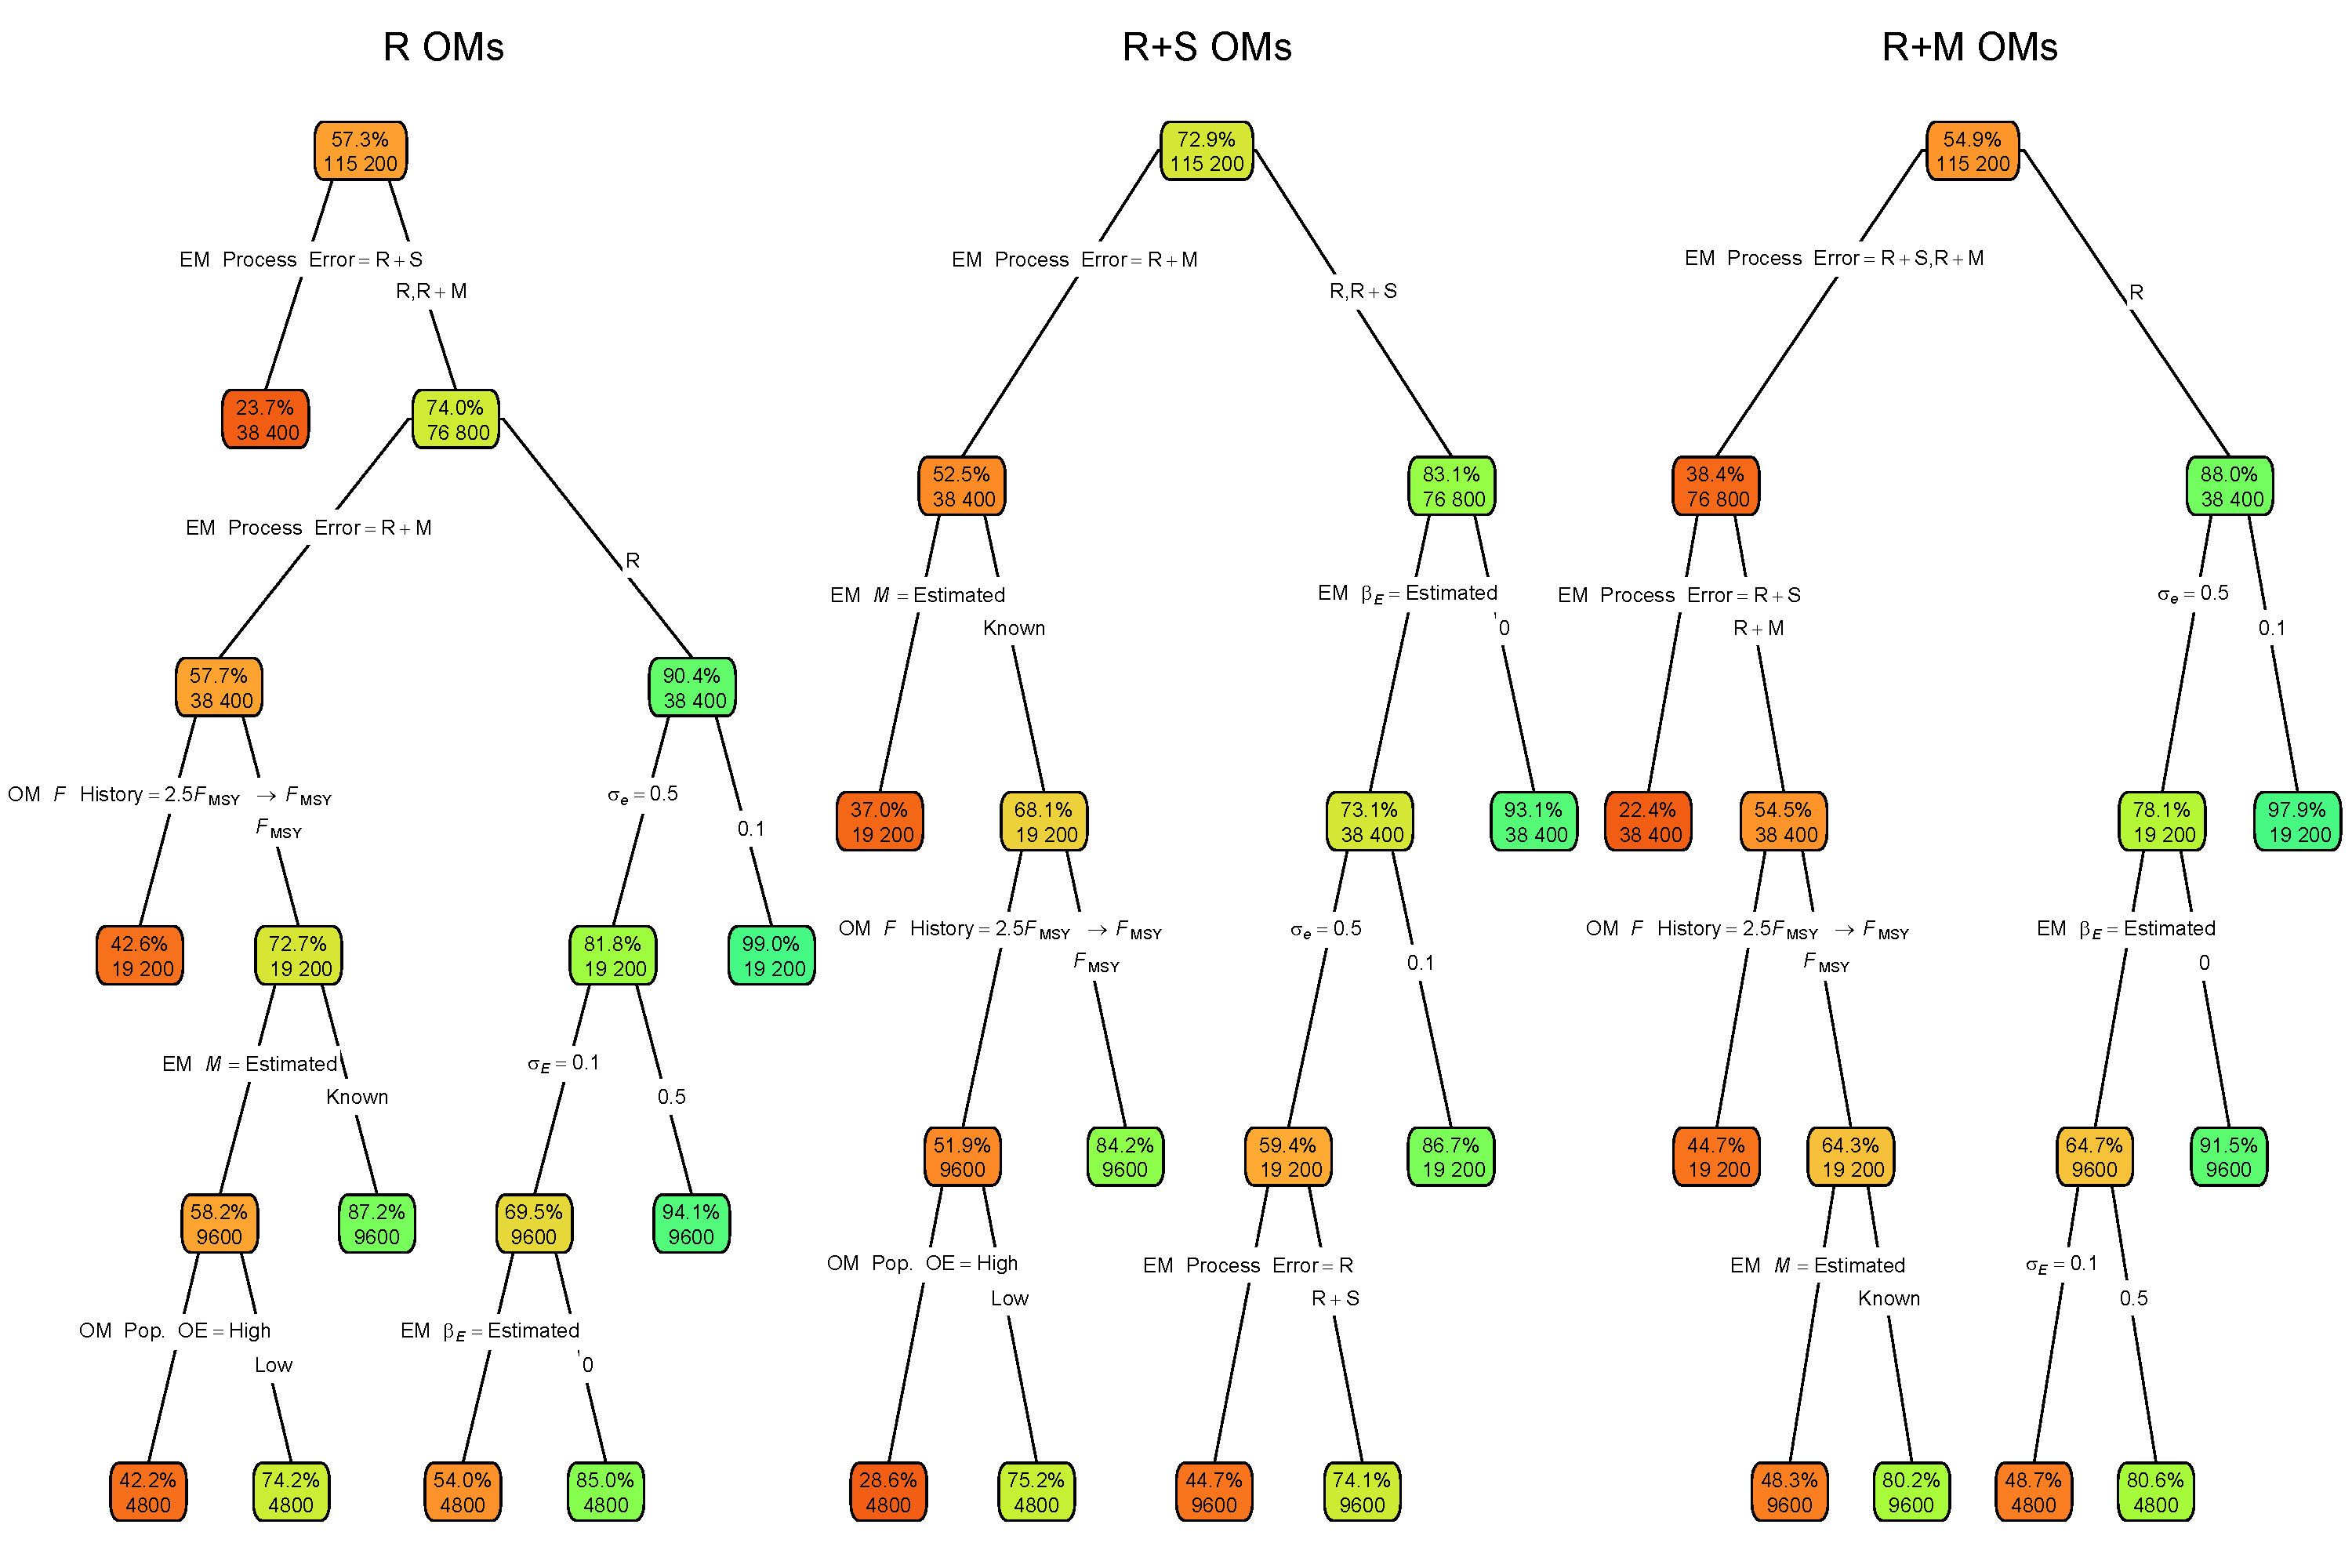
\includegraphics[width = 1.4\textwidth]{convergence_classification_plots}
\end{center}
\caption{Classification trees indicating primary factors determining convergence as defined by providing Hessian-based standard errors for operating models (OMs) with process error on recruitment only (R), recruitment and apparent survival (R+S), or recruitment and natural mortality (R+M). Nodes denote percent convergence (top) and number of fits (bottom) for the corresponding subset. Lower or higher convergence rates are indicated by more red or green polygons, respectively. See Table \ref{factor_table} for description of OM and estimating model (EM) factors defining nodes and branches.}\label{conv_class}
\end{figure}
\end{landscape}

\begin{landscape}
\begin{figure}
\begin{center}
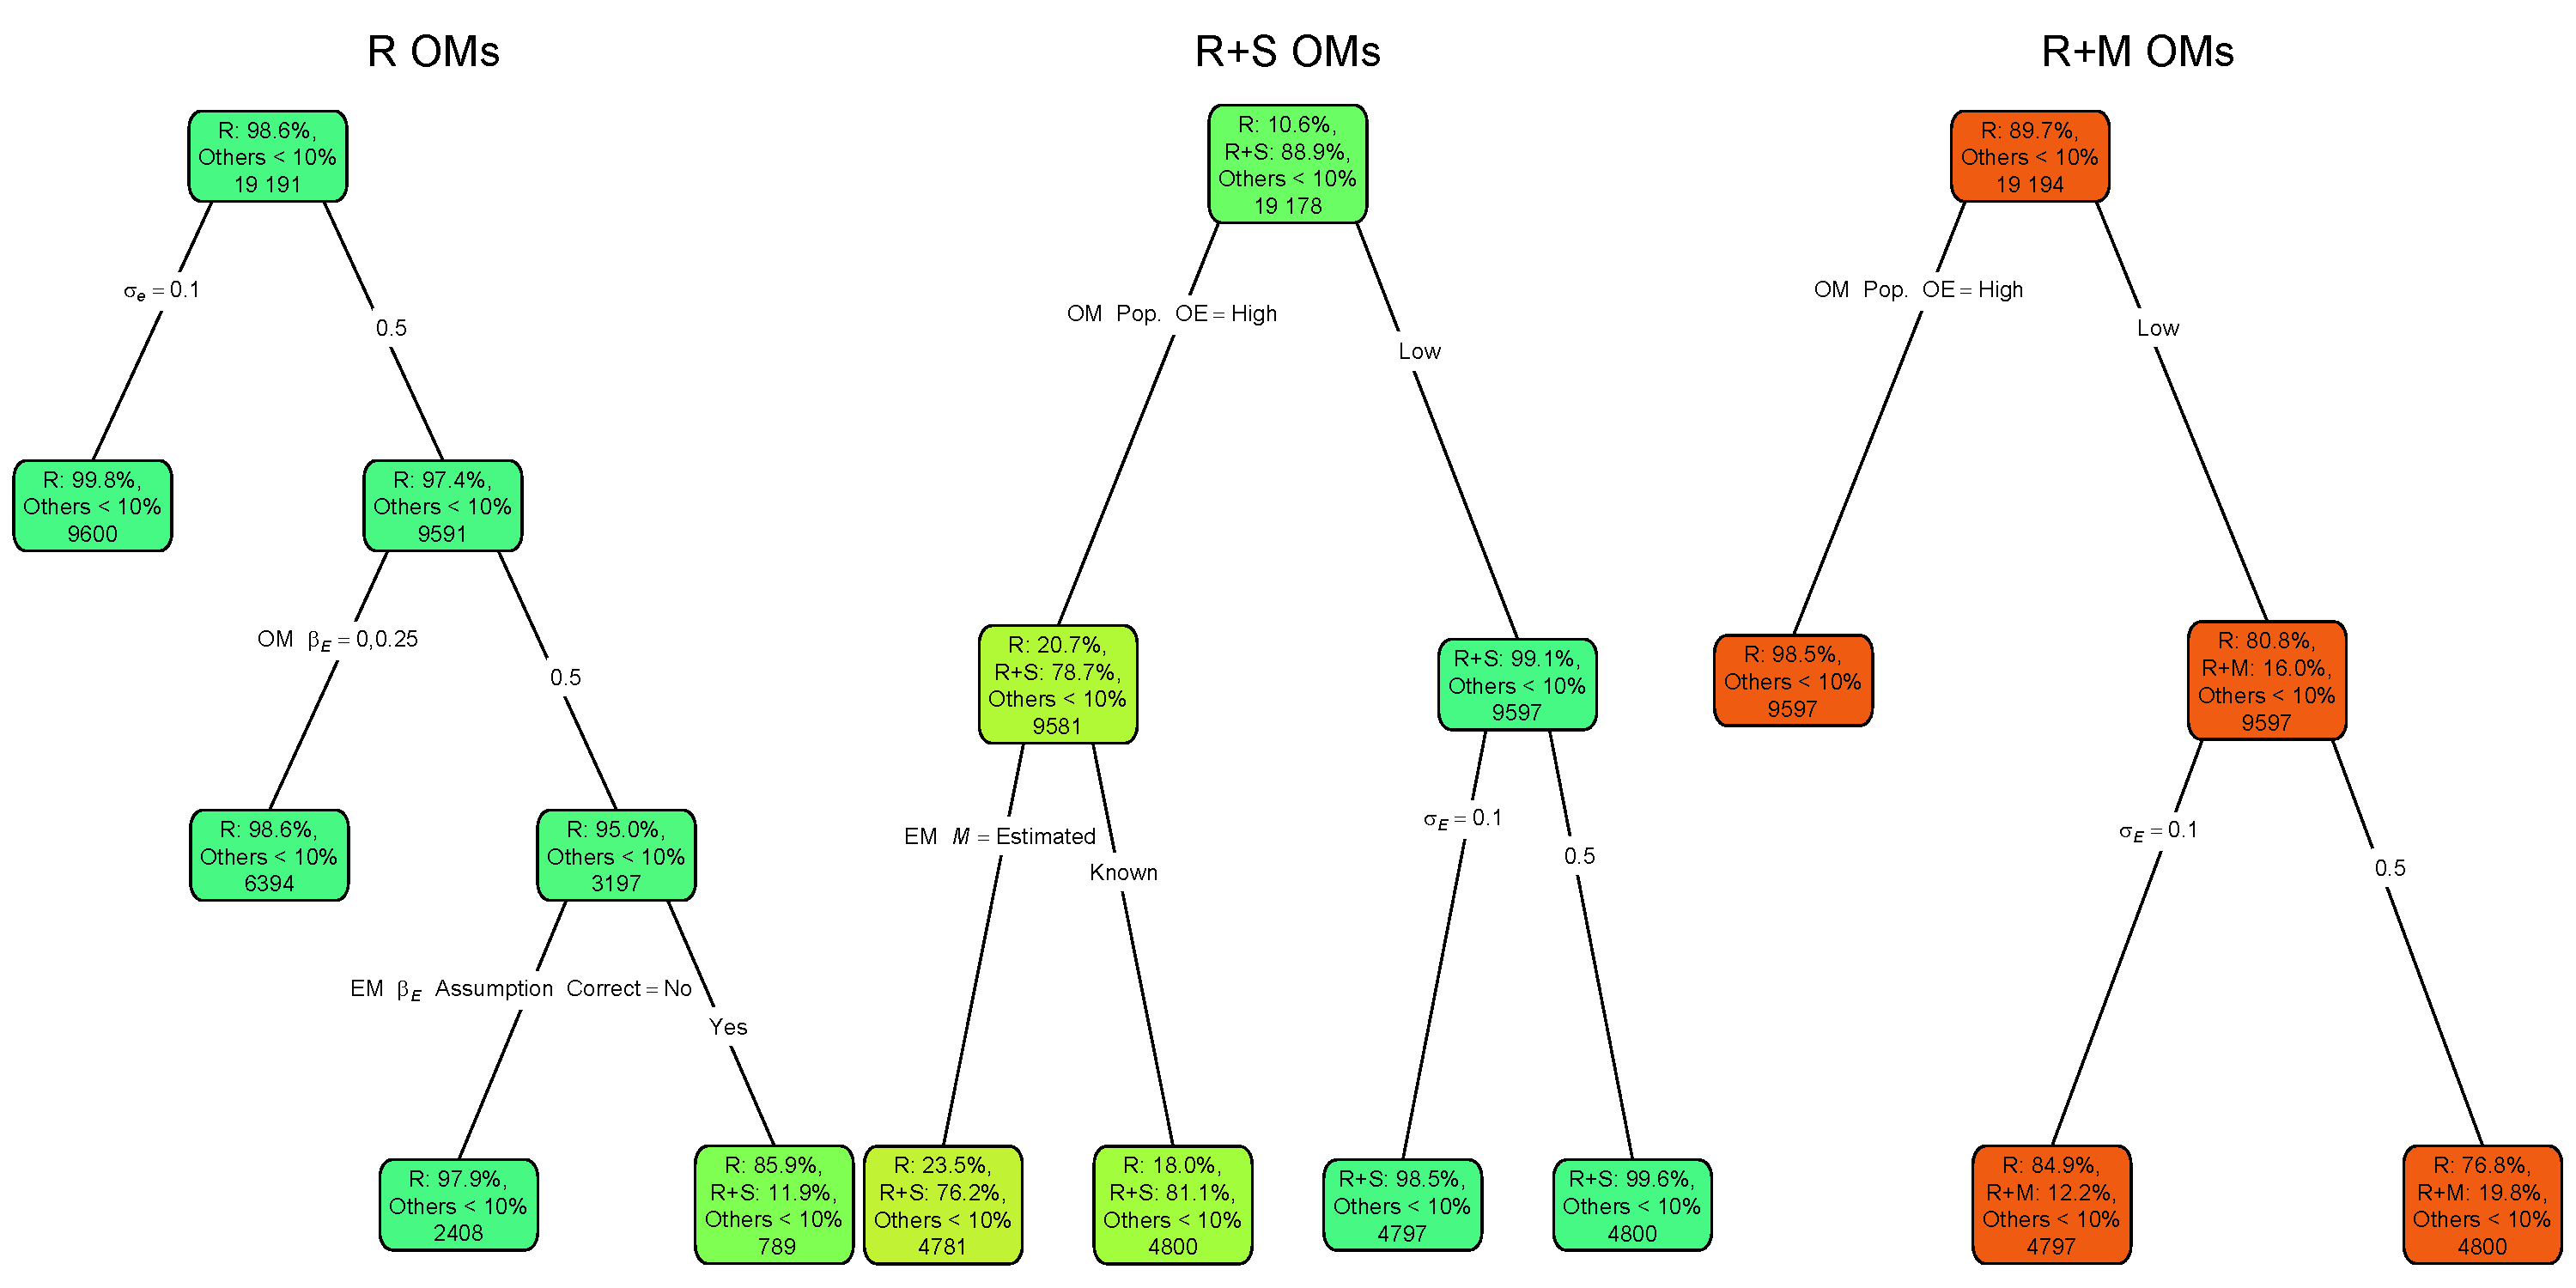
\includegraphics[width = 1.4\textwidth]{AIC_PE_classification_plots}
\end{center}
\caption{Classification trees for which estimating model process error assumption provides the lowest AIC. Each node shows the percentages (if greater than 10\%) of estimating model fits with a given process error assumption having the lowest AIC for the corresponding subset. Process error assumptions with percentages less than 10\% are grouped as ``other.'' Lower or higher accuracy are indicated by more red or green polygons, respectively. See Figure \ref{conv_class} caption and Table \ref{factor_table} for further details.}\label{AIC_PE_class}
\end{figure}
\end{landscape}

\begin{landscape}
\begin{figure}
\begin{center}
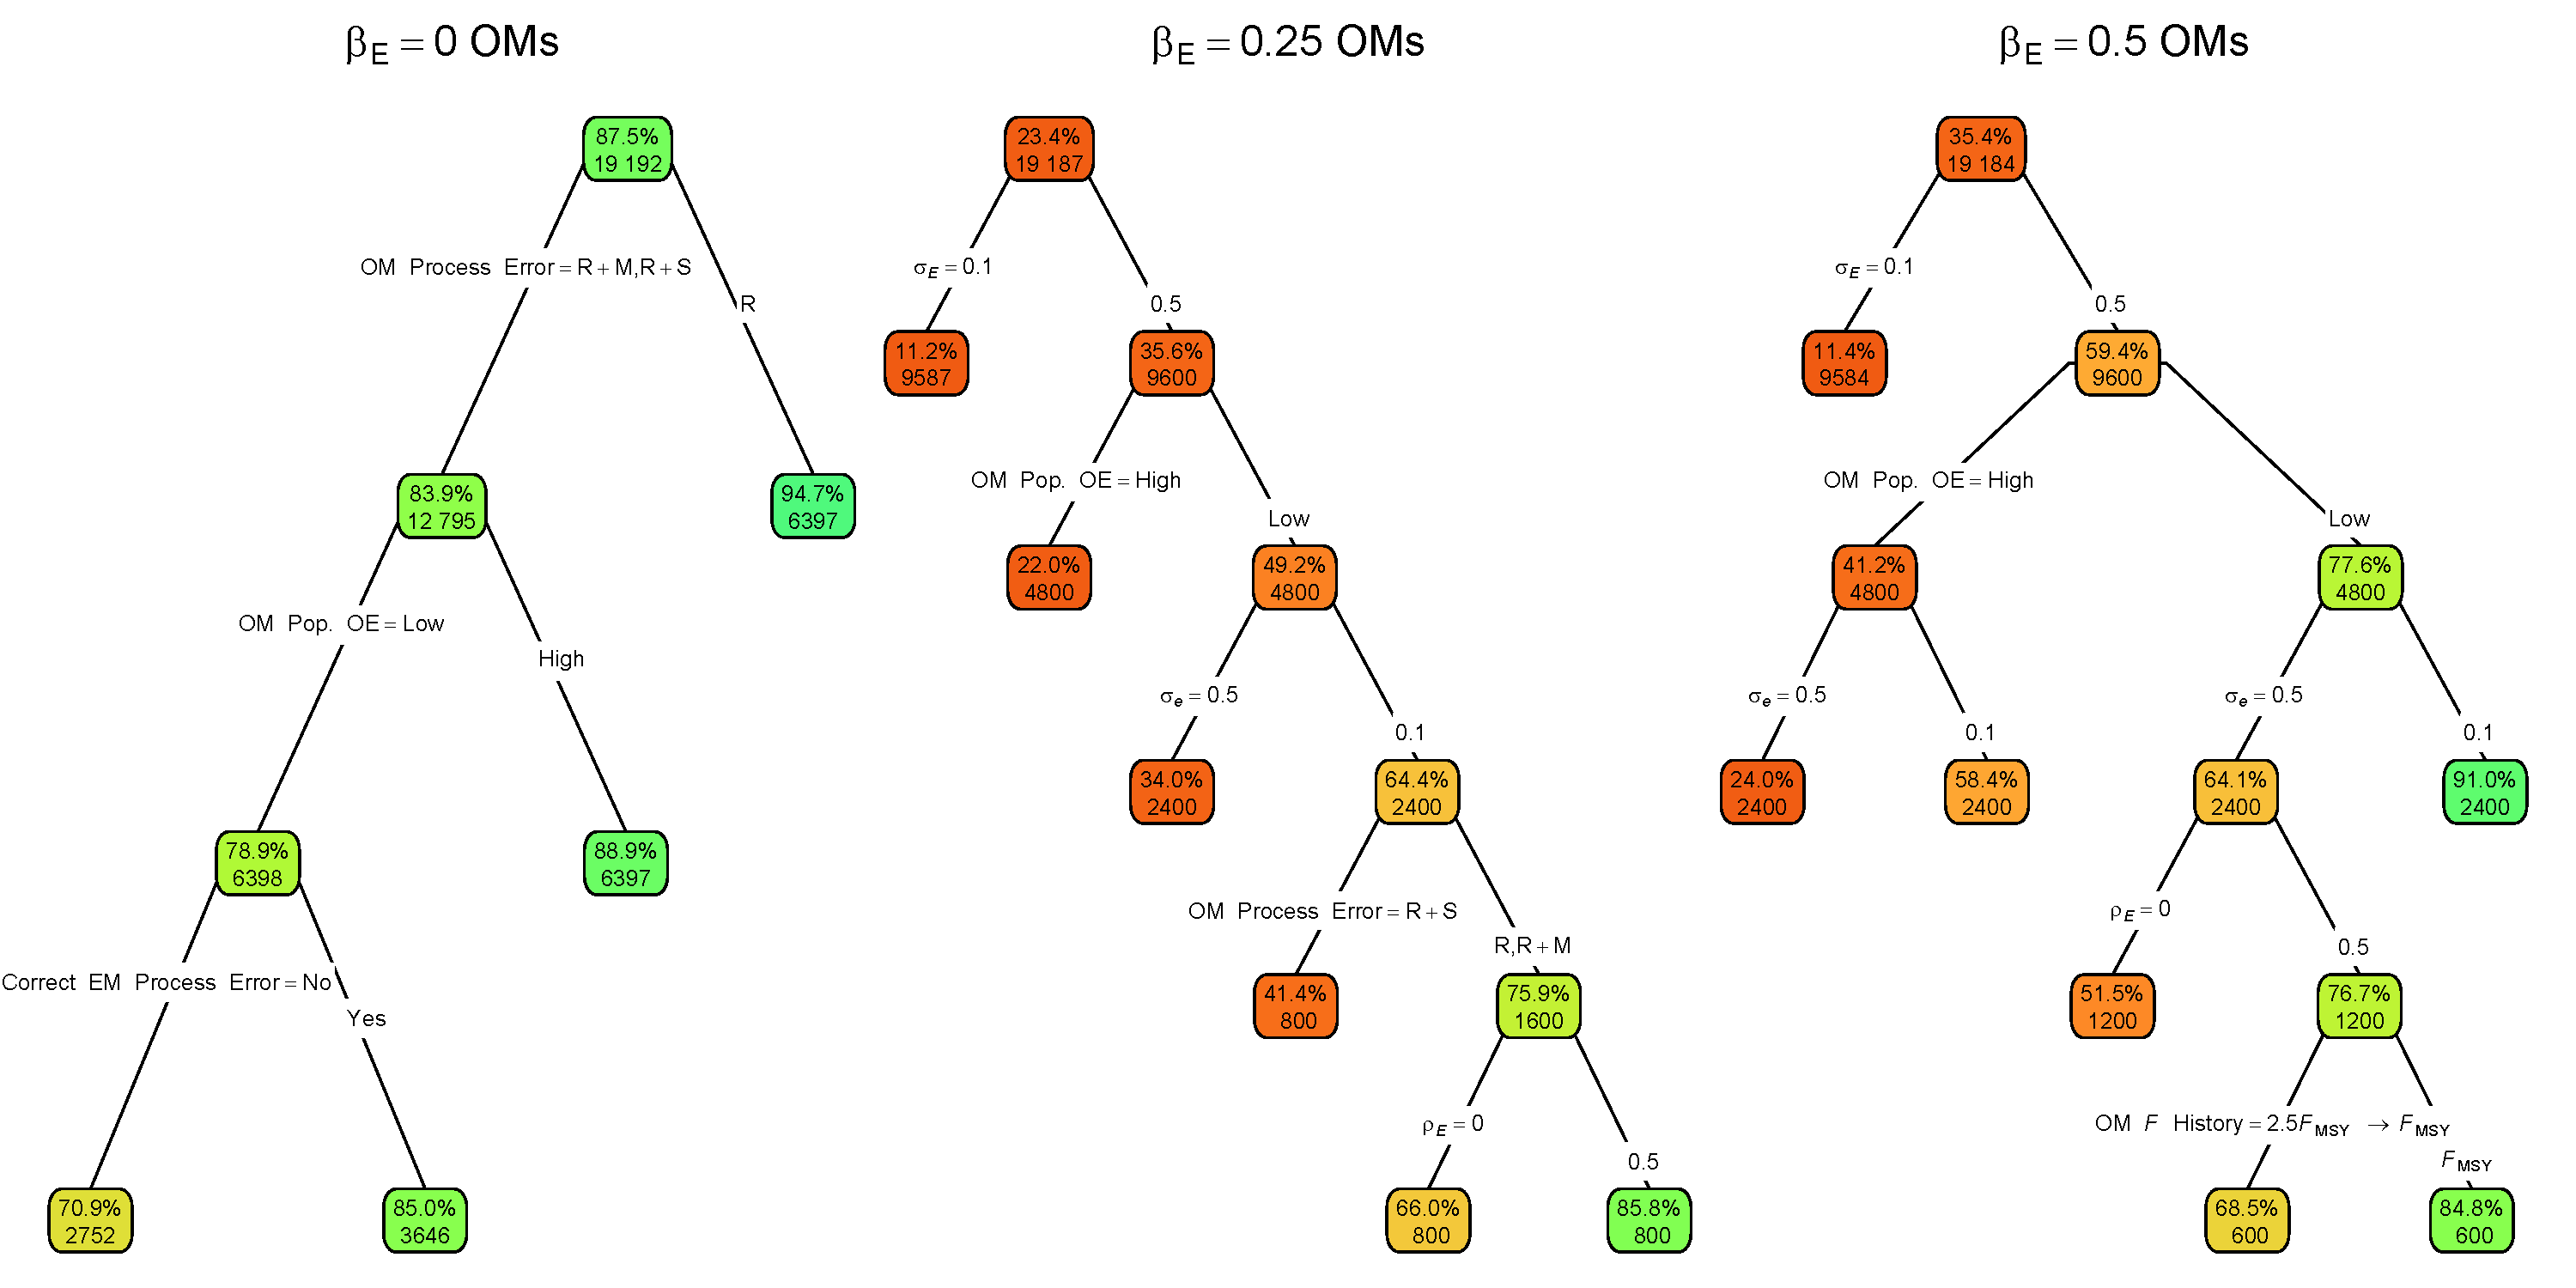
\includegraphics[width = 1.4\textwidth]{AIC_Ecov_effect_classification_plots}
\end{center}
\caption{Classification trees for whether the correct estimating model assumption for covariate effect on $M$ (no effect with OM $\beta_E = 0$ or estimated effect when OM $\beta_E > 0$) provides the lowest AIC for OMs assuming values for $\beta_E$ of 0, 0.25, and 0.5. Nodes denote the percentage of estimating models with the correct assumption and lowest AIC  for the corresponding subset. Lower or higher accuracy are indicated by more red or green polygons, respectively. See Figure \ref{conv_class} caption and Table \ref{factor_table} for further details.}\label{AIC_Ecov_effect_class}
\end{figure}
\end{landscape}

\begin{landscape}
\begin{figure}
\begin{center}
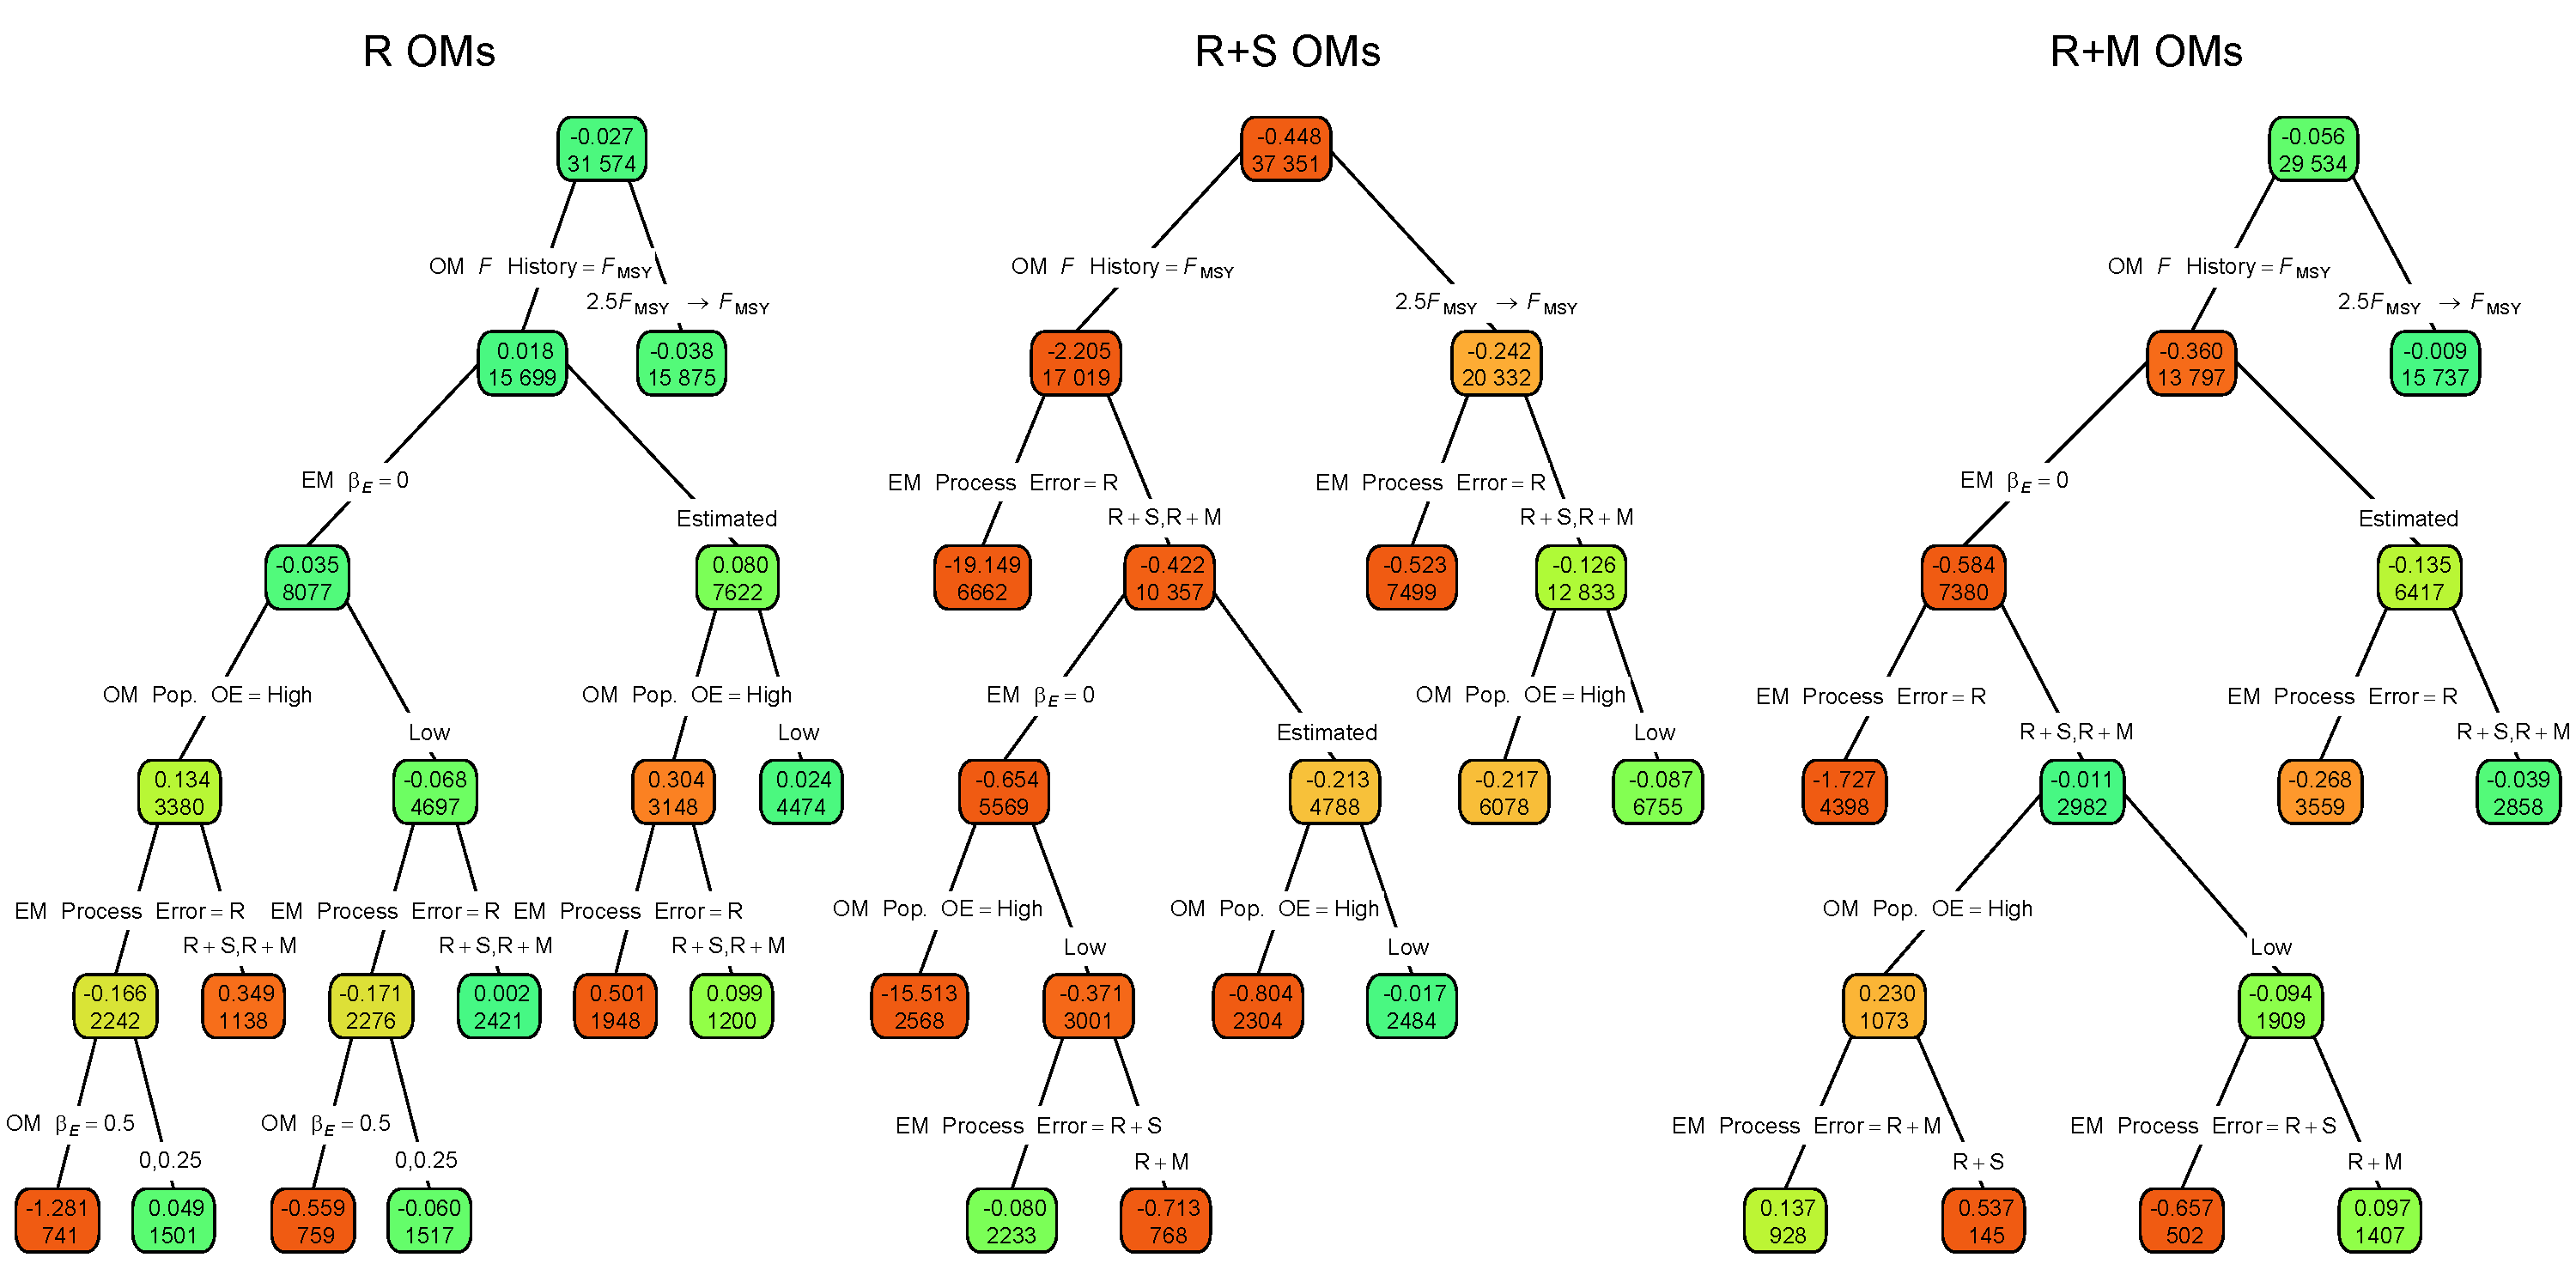
\includegraphics[width = 1.4\textwidth]{median_M_bias_regtree_plots}
\end{center}
\caption{Regression trees for estimation error of the median $M$ parameter ($\beta_M$). Each node shows the median error for the corresponding subset. Lower or higher absolute median errors are indicated by more green or red polygons, respectively. See Figure \ref{conv_class} caption and Table \ref{factor_table} for further details.}\label{med_M_bias_regtree}
\end{figure}
\end{landscape}

\begin{landscape}
\begin{figure}
\begin{center}
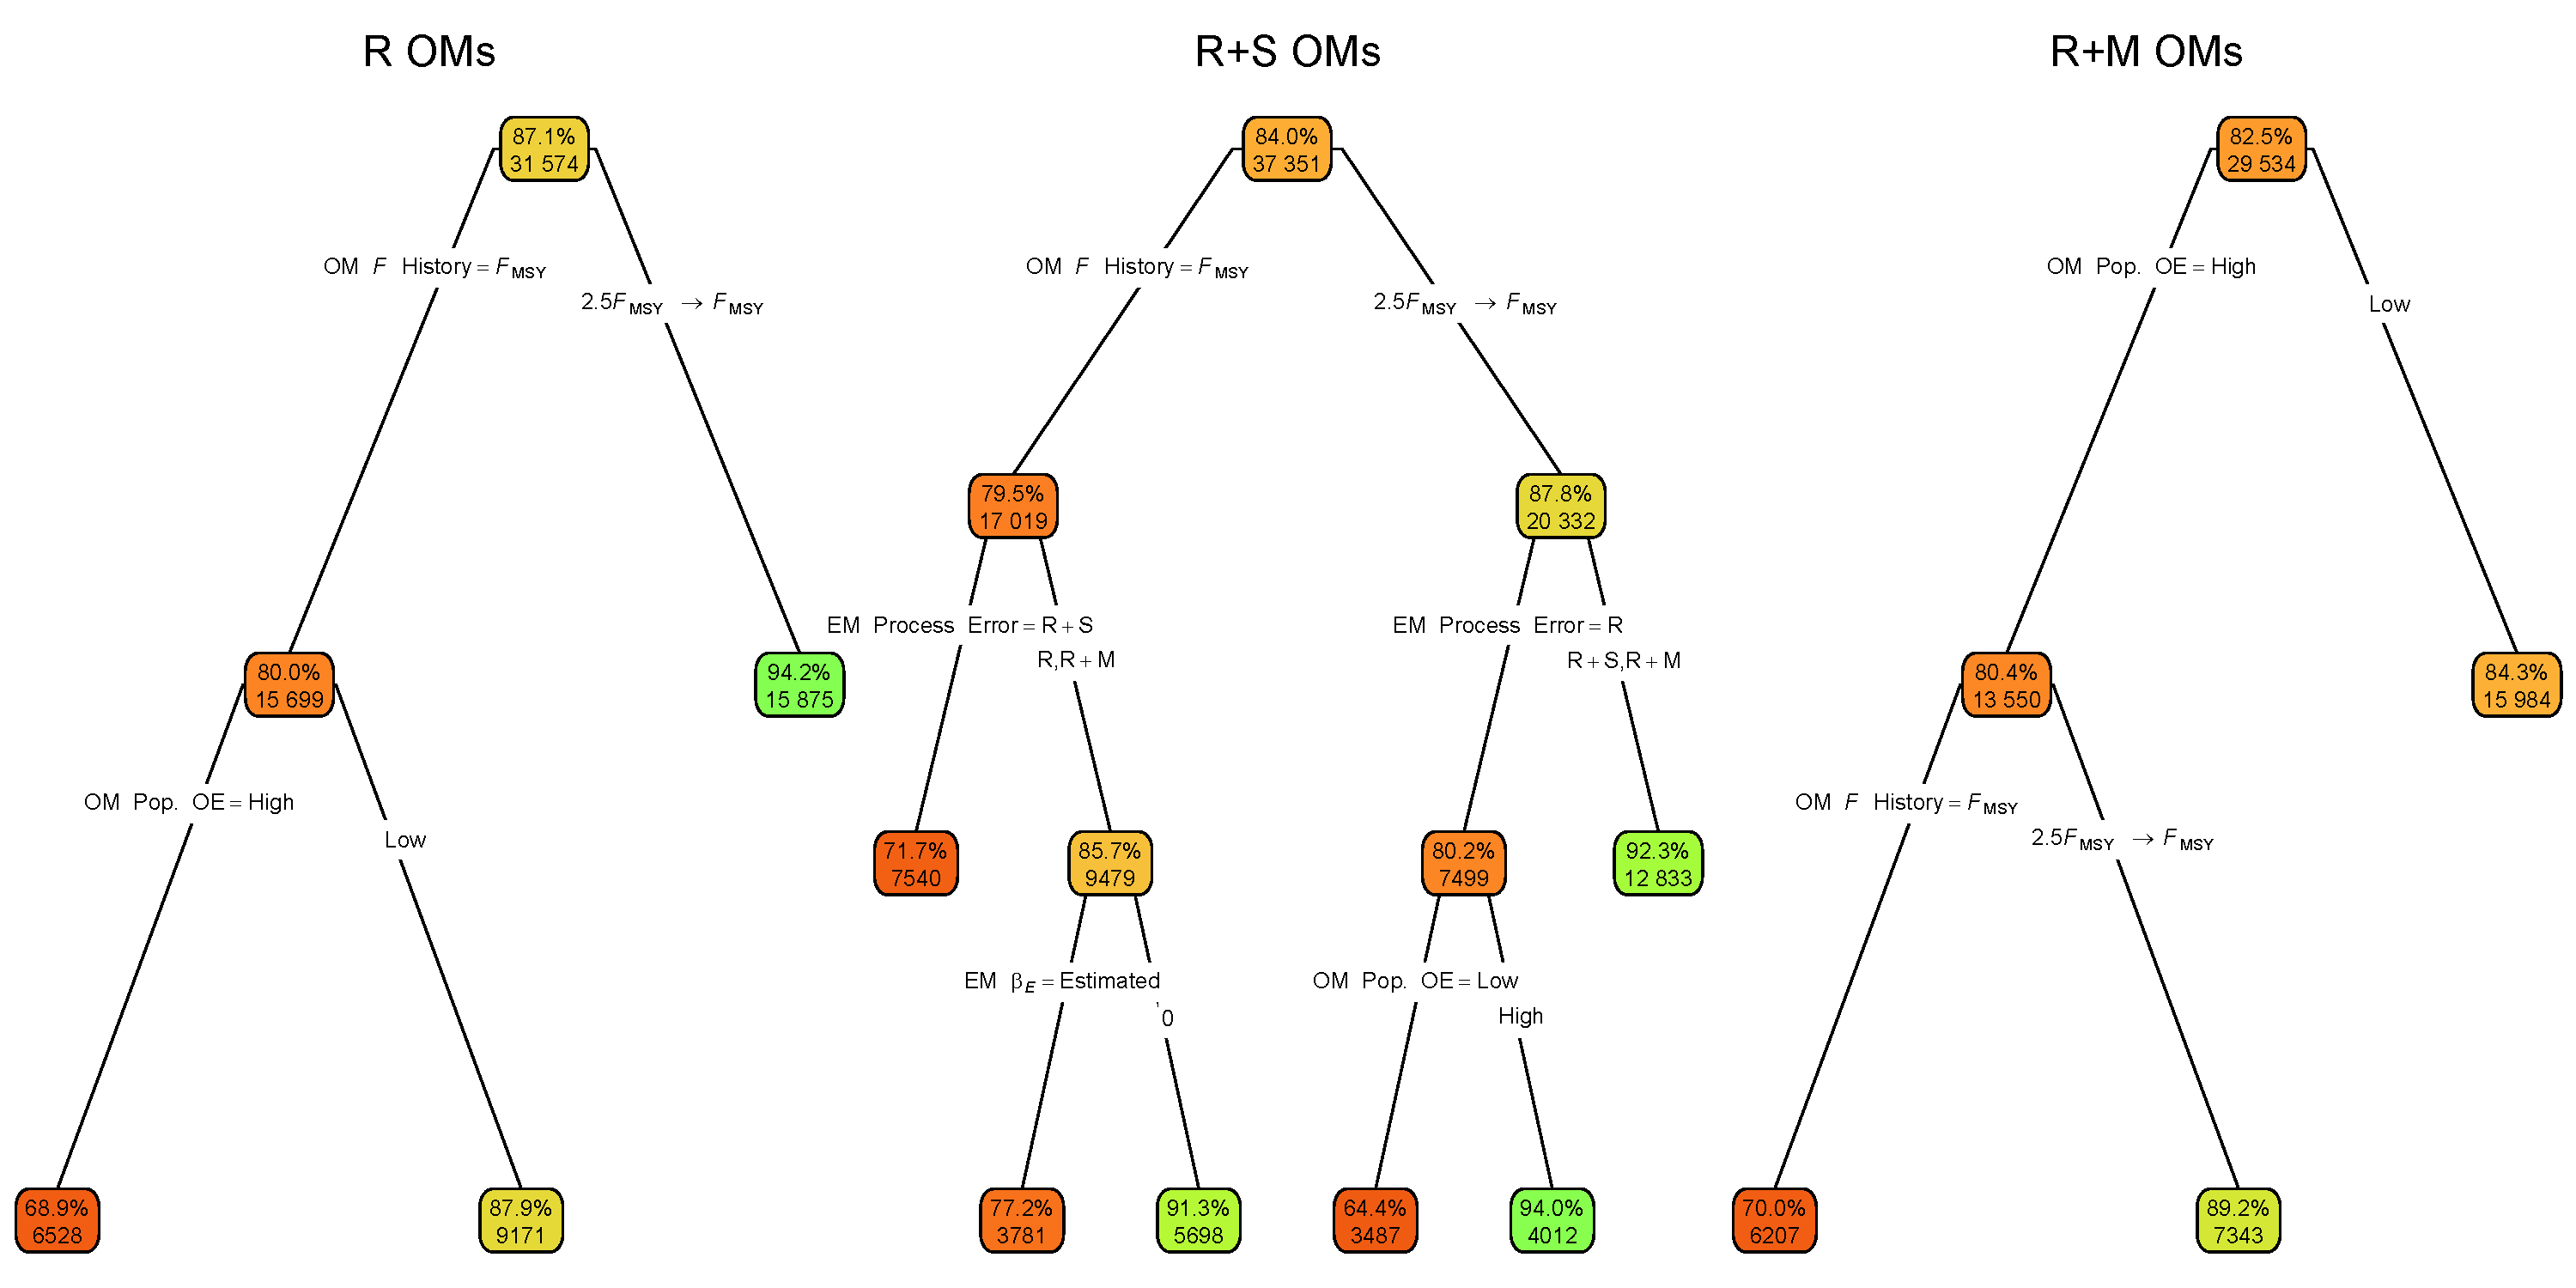
\includegraphics[width = 1.4\textwidth]{median_M_CI_coverage_regtree_plots}
\end{center}
\caption{Classification trees for whether confidence intervals (CIs) for the estimated median $M$ parameter ($\beta_M$) included the true value. Each node shows the percentage of CIs that include the true value for the corresponding subset. Higher or lower percentages are indicated by more green or red polygons, respectively. See Figure \ref{conv_class} caption and Table \ref{factor_table} for further details.}\label{med_M_CI_coverage_regtree}
\end{figure}
\end{landscape}

\begin{landscape}
\begin{figure}
\begin{center}
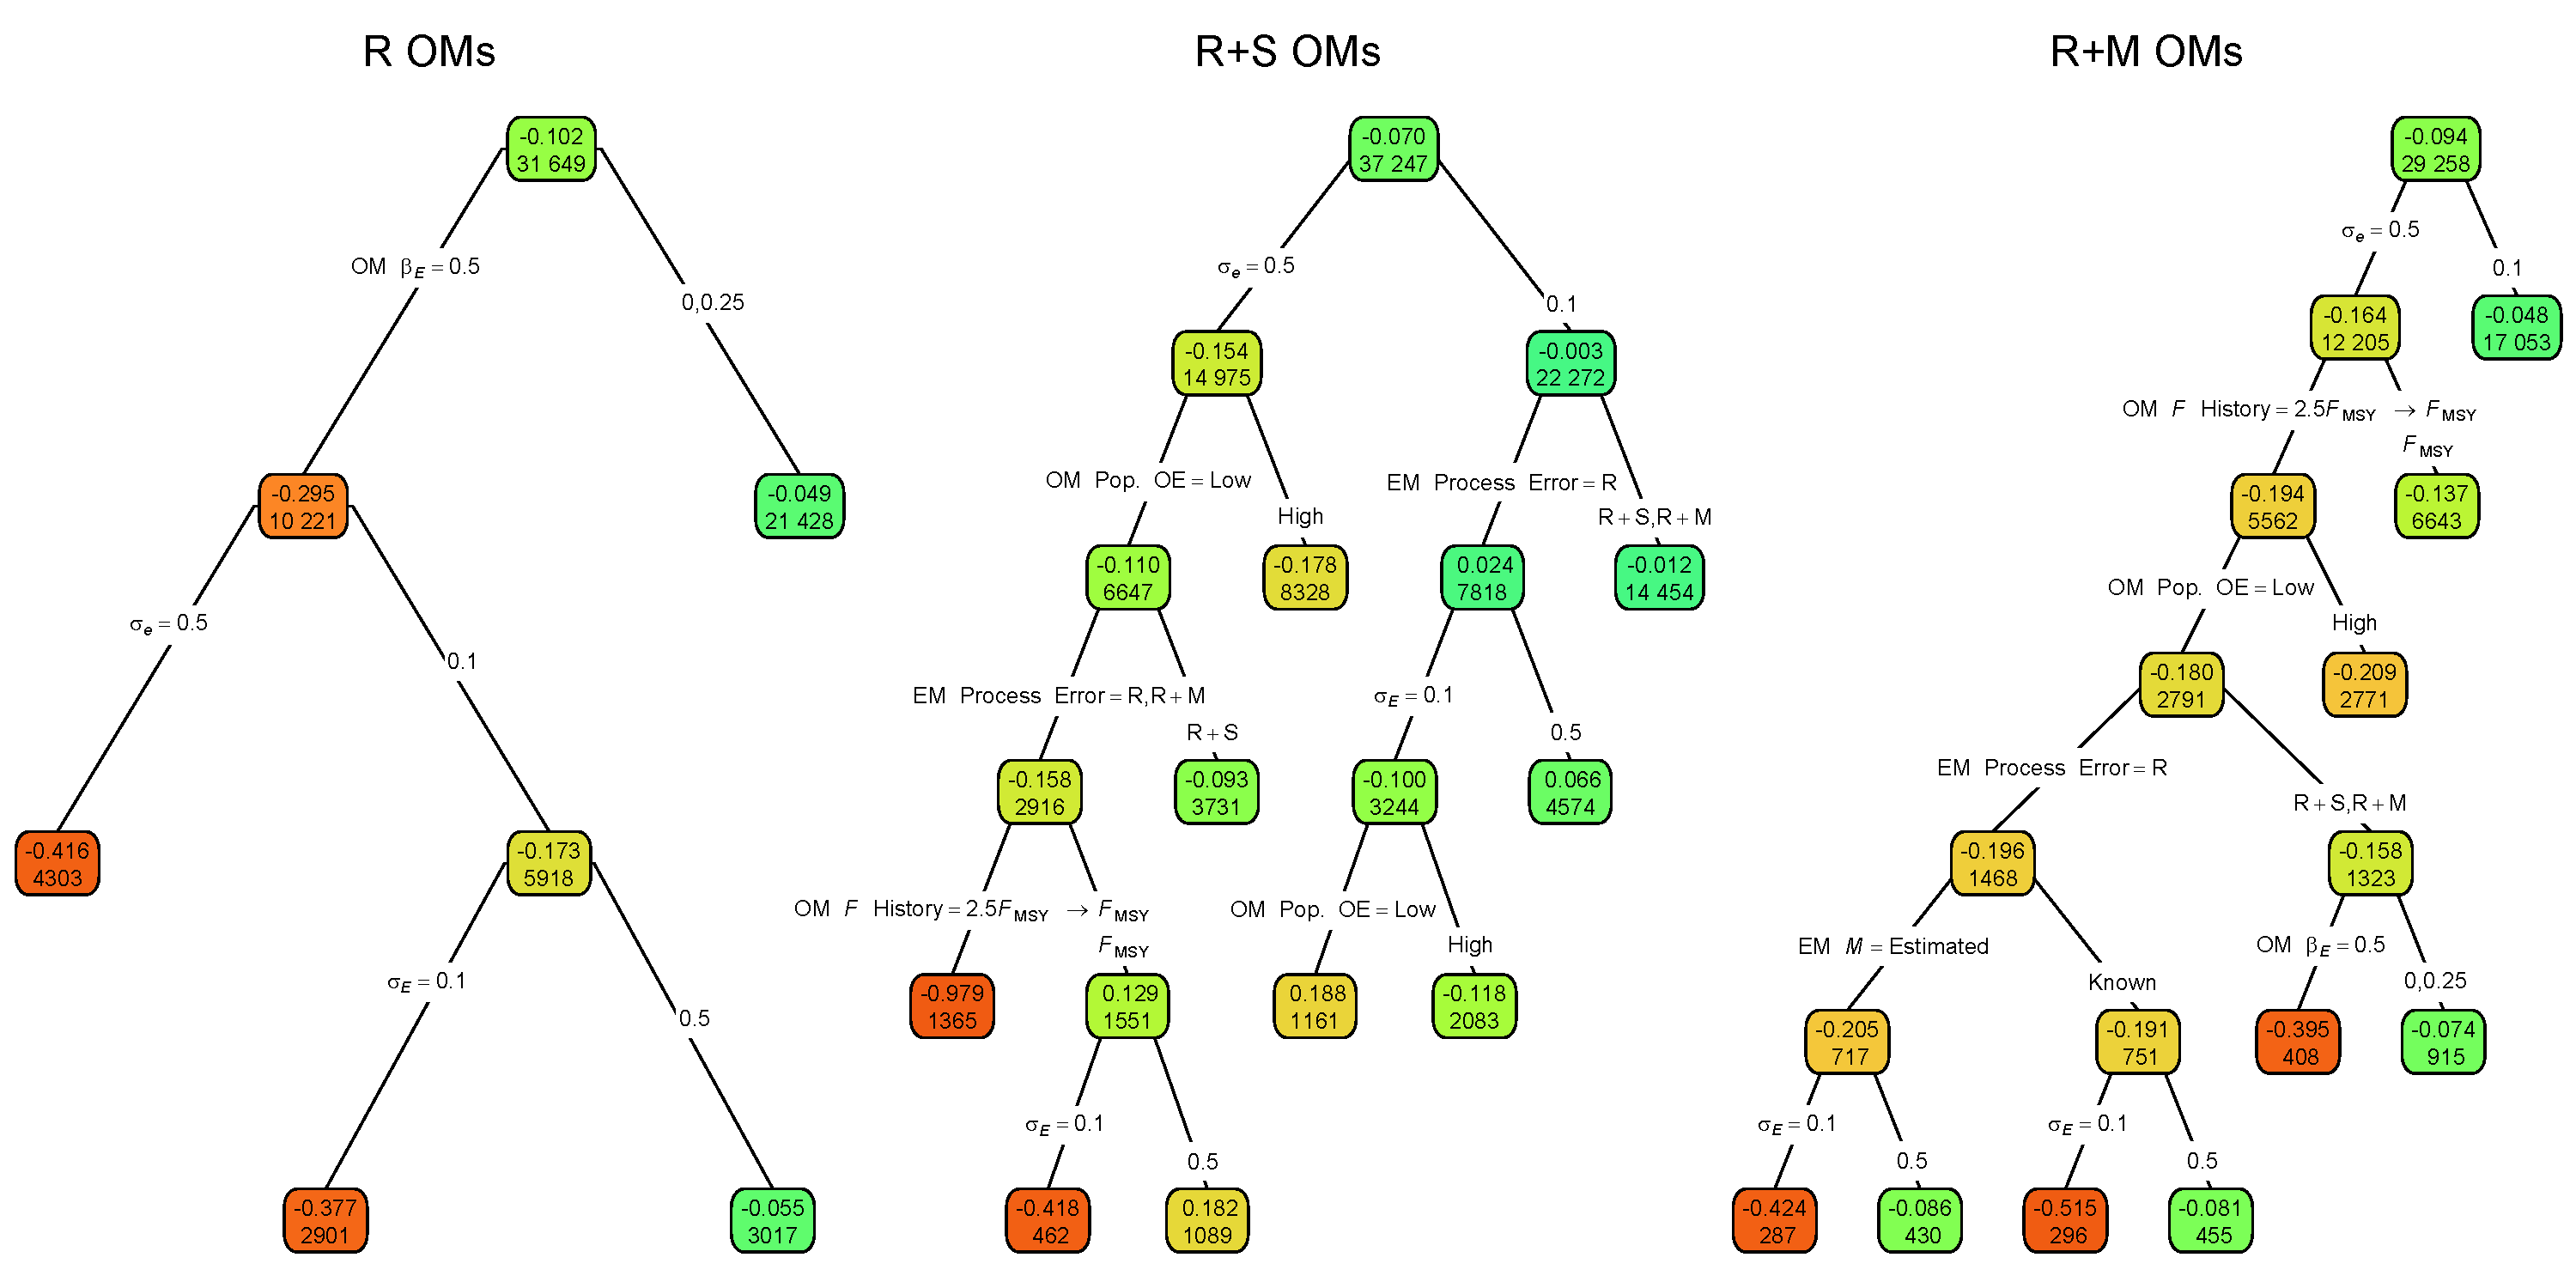
\includegraphics[width = 1.4\textwidth]{ecov_beta_bias_regtree_plots}
\end{center}
\caption{Regression trees for estimation error of the covariate effect on $M$ ($\widehat \beta_E$). Each node shows the median error (top) for the corresponding subset. Lower or higher absolute median error are indicated by more green or red polygons, respectively. See Figure \ref{conv_class} caption and Table \ref{factor_table} for further details.}\label{ecov_effect_bias_regtree}
\end{figure}
\end{landscape}

\begin{landscape}
\begin{figure}
\begin{center}
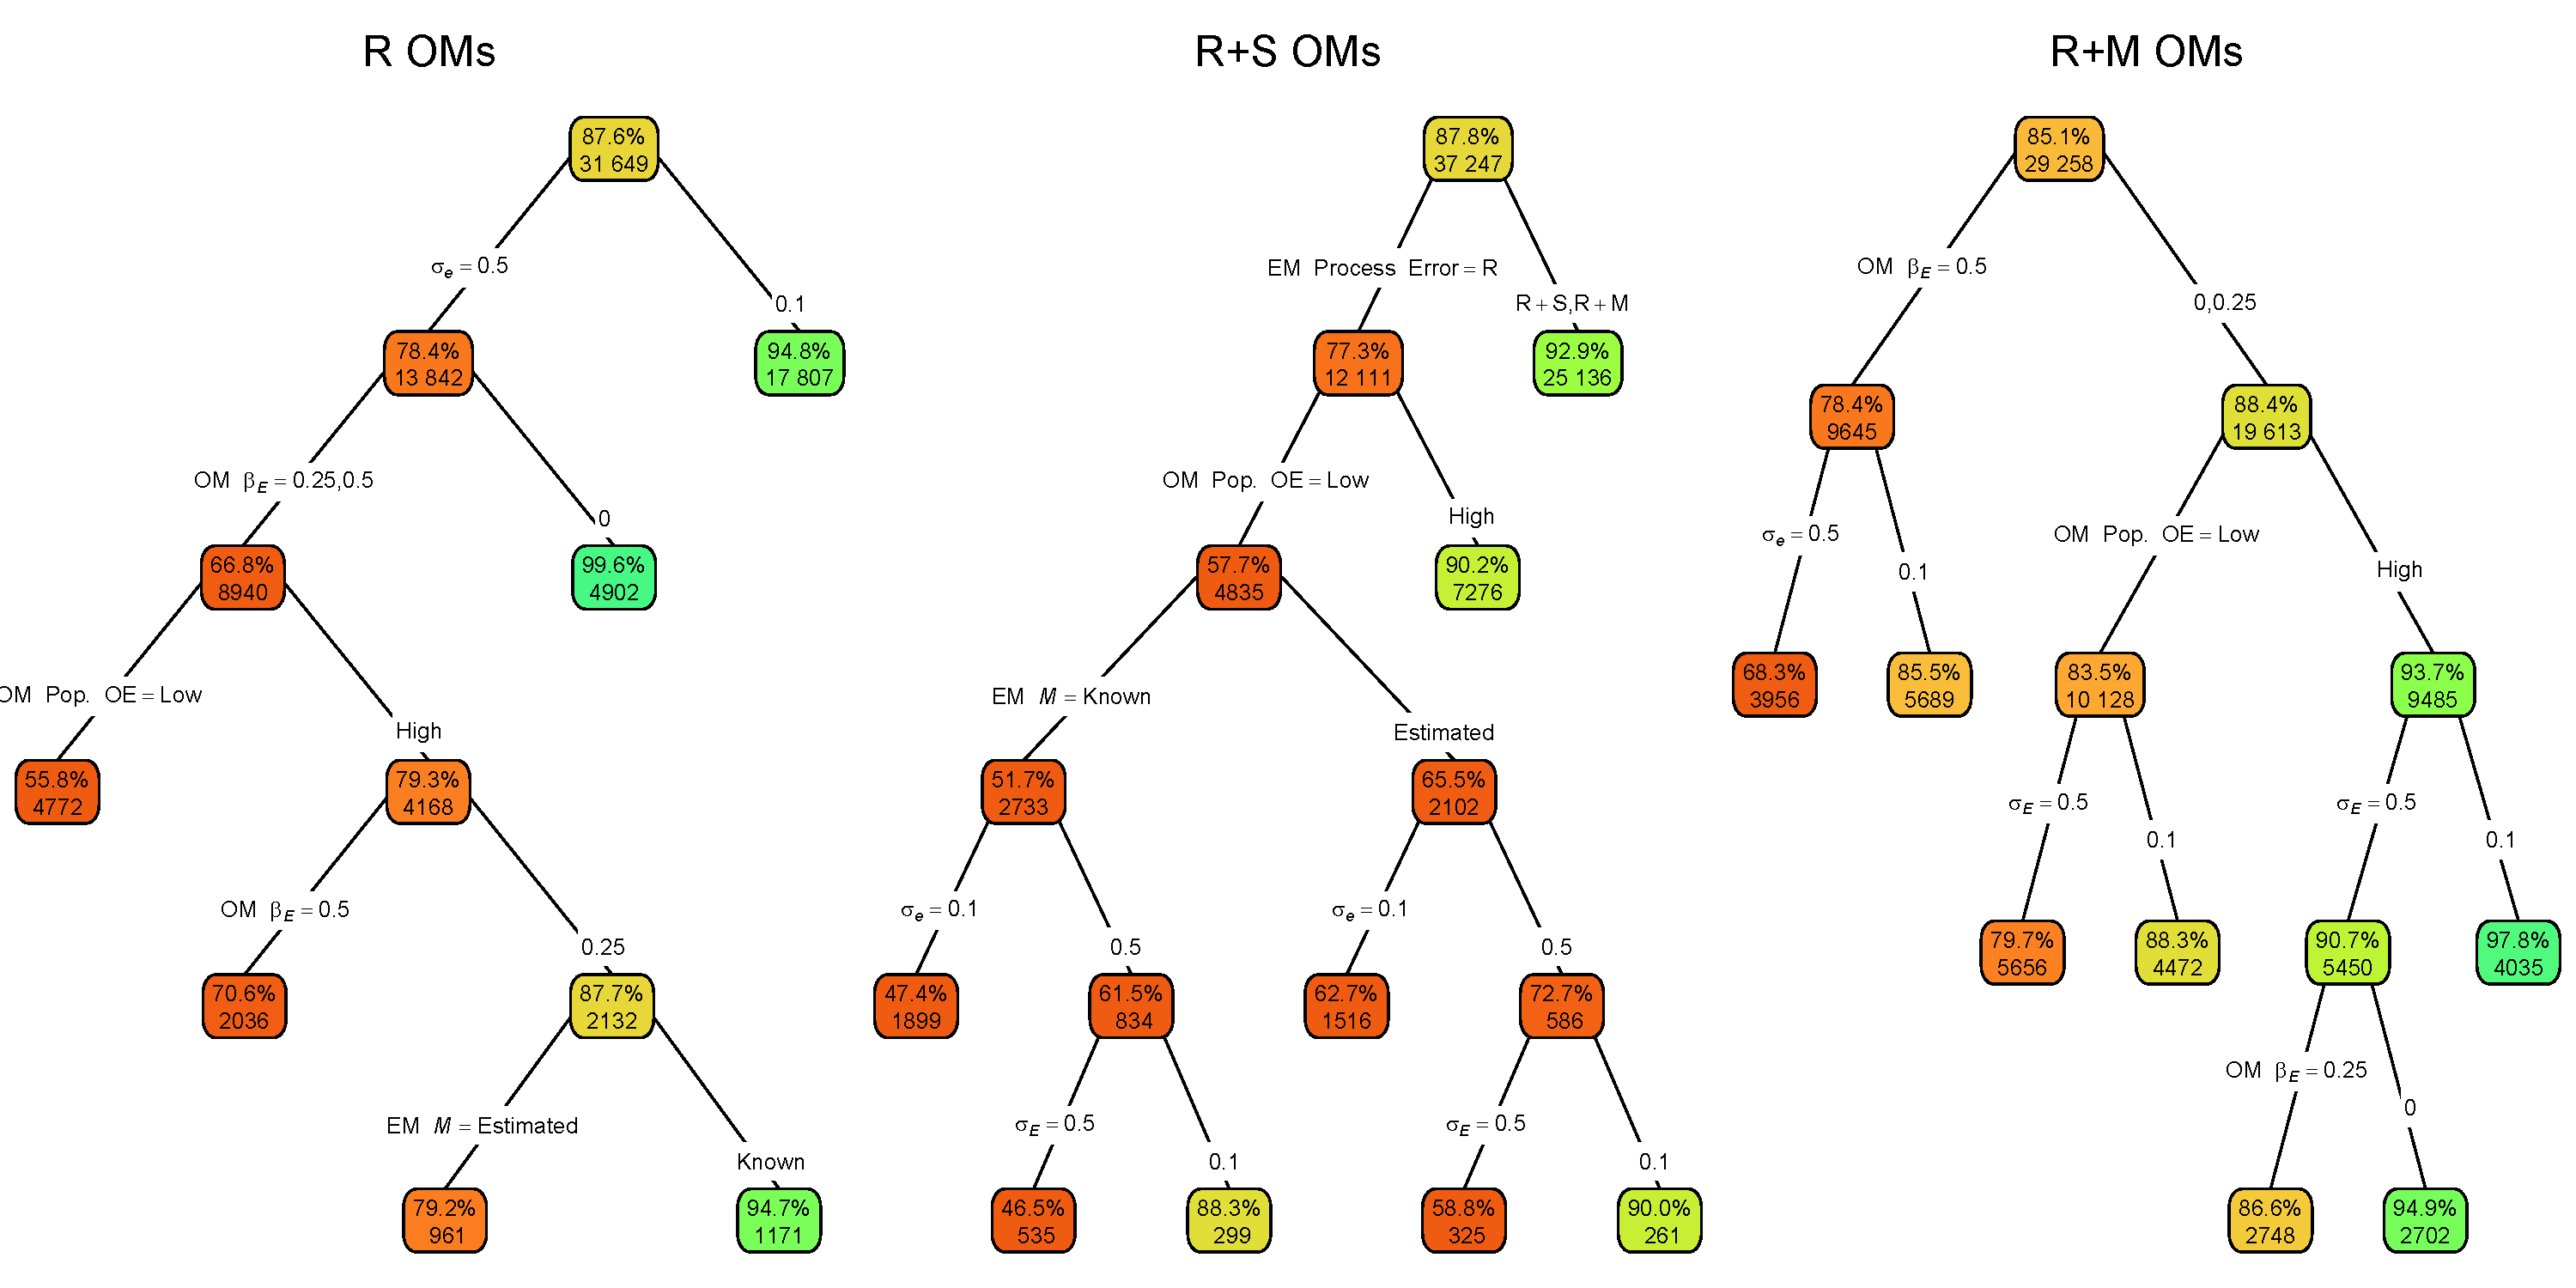
\includegraphics[width = 1.4\textwidth]{ecov_beta_CI_coverage_regtree_plots}
\end{center}
\caption{Classification trees for whether confidence intervals (CIs) for the estimated covariate effects on $M$ ($\beta_E$) included the true value. Each node shows the percentage of CIs that include the true value for the corresponding subset. Higher or lower percentages are indicated by more green or red polygons, respectively. See Figure \ref{conv_class} caption and Table \ref{factor_table} for further details.}\label{ecov_effect_CI_coverage_regtree}
\end{figure}
\end{landscape}

\begin{landscape}
\begin{figure}
\begin{center}
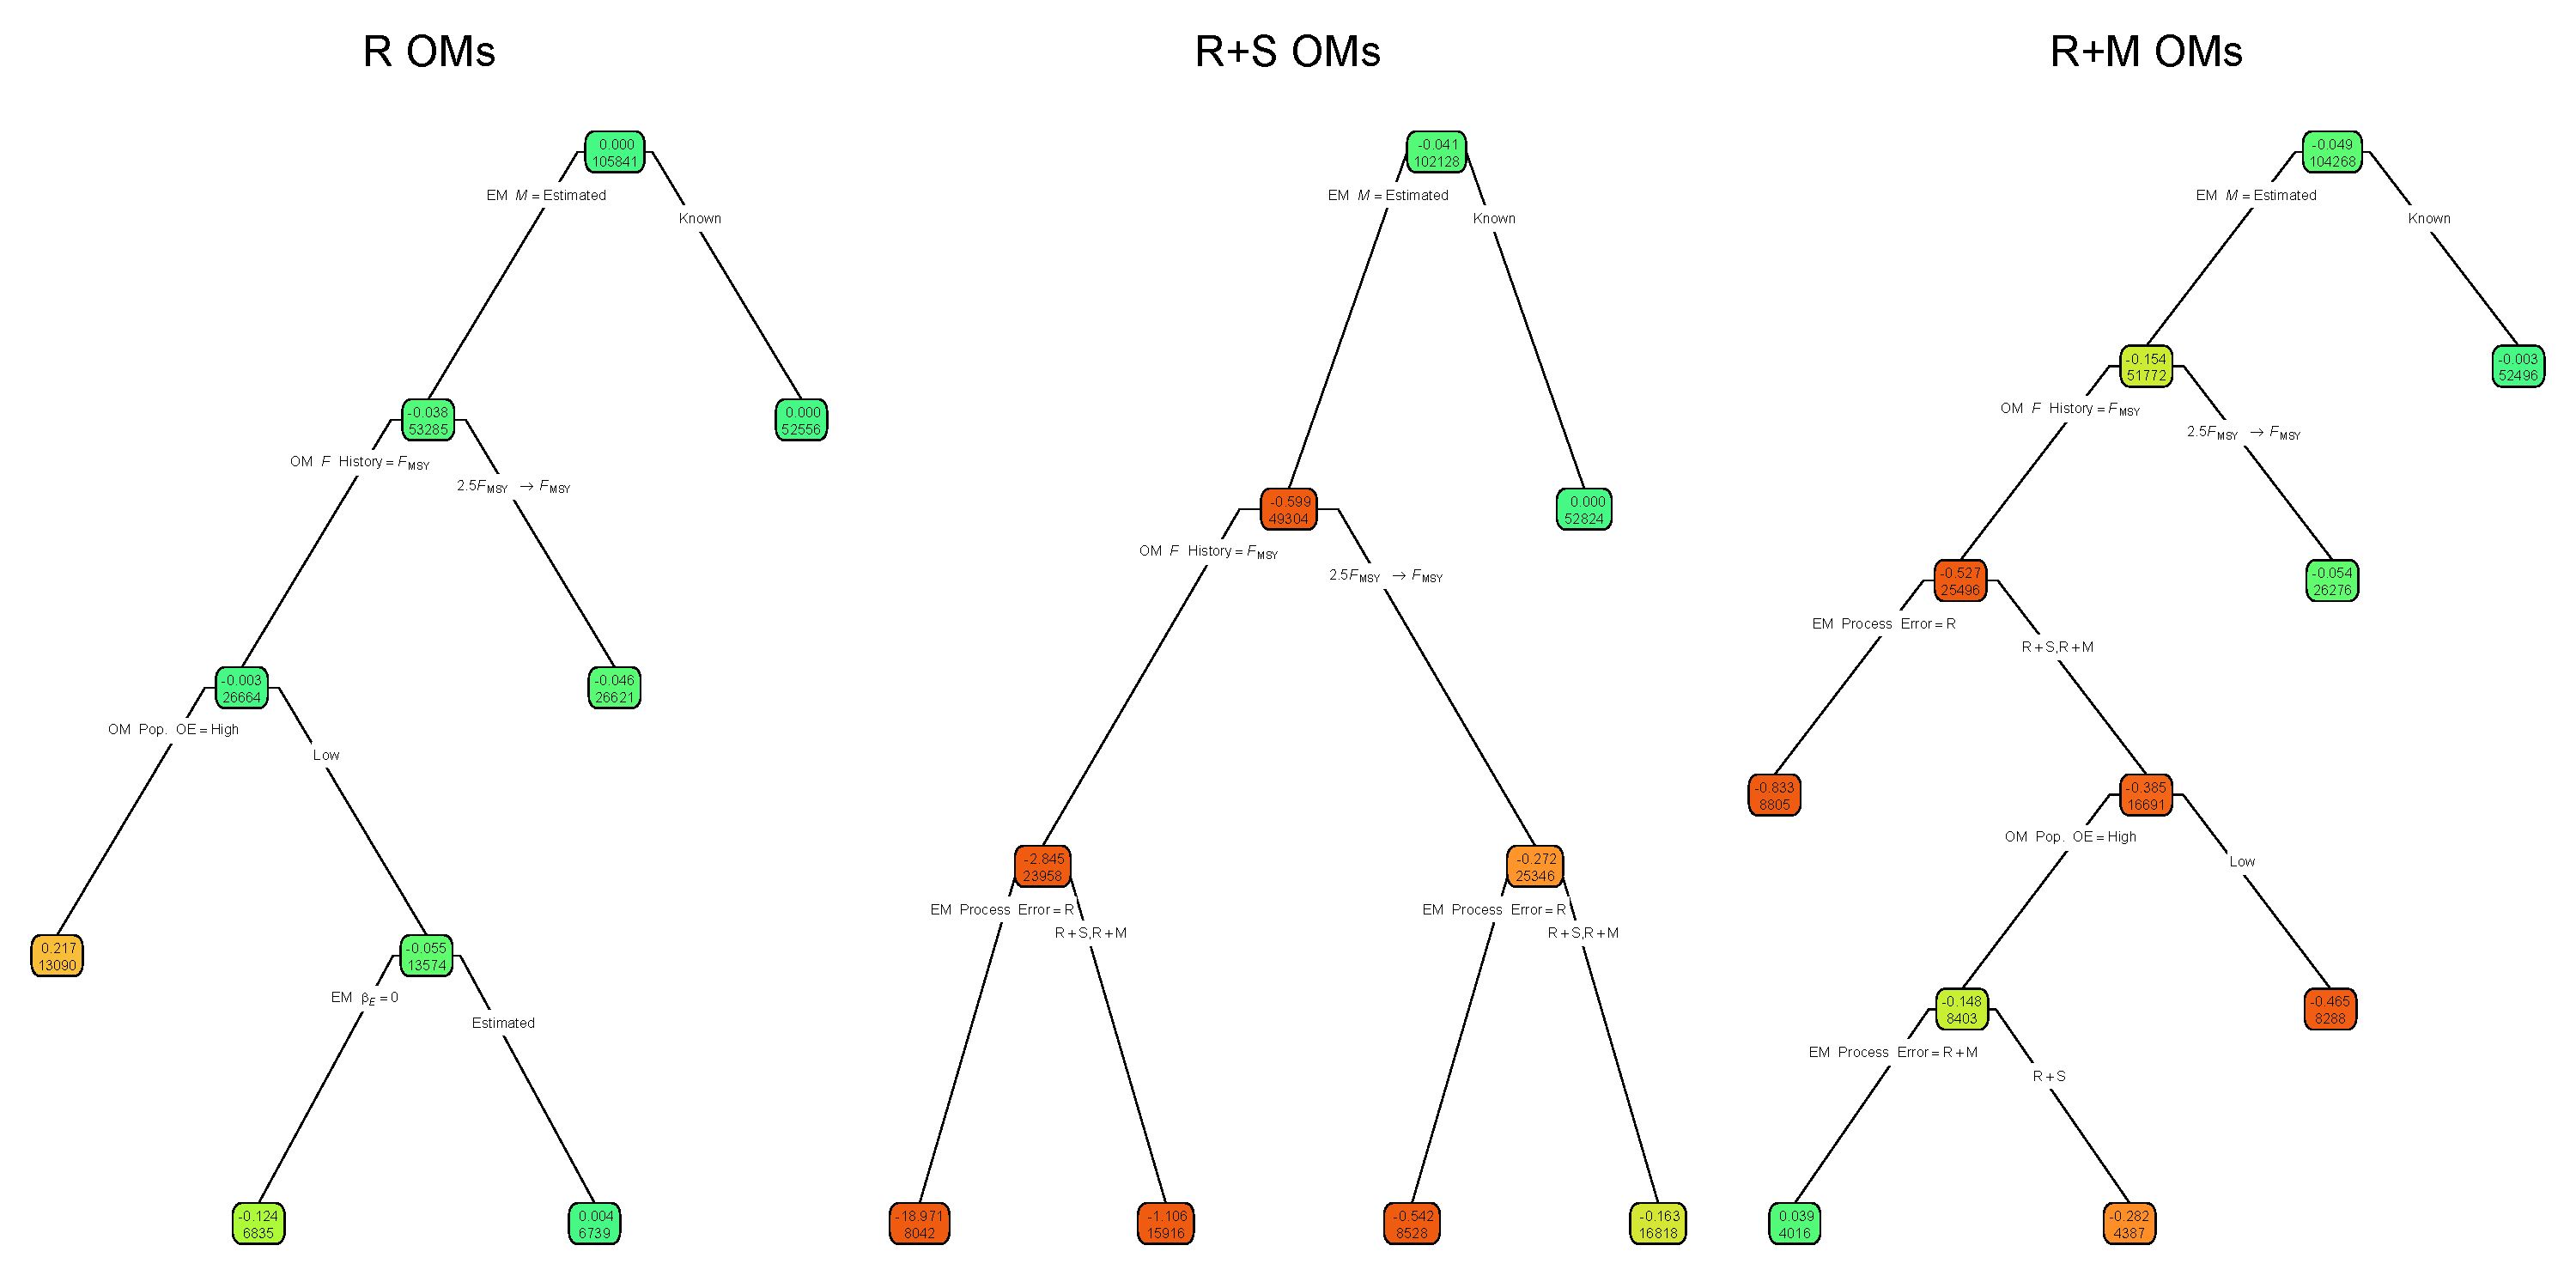
\includegraphics[width = 1.4\textwidth]{term_M_bias_regtree_plots}
\end{center}
\caption{Regression trees for estimation error of terminal year $M$ as measured by Eq. \ref{relerror_trans_response}. Each node shows the median error for the corresponding subset. Lower or higher absolute median errors are indicated by more green or red polygons, respectively. See Figure \ref{conv_class} caption and Table \ref{factor_table} for further details.}\label{term_M_bias_regtree}
\end{figure}
\end{landscape}

\begin{landscape}
\begin{figure}
\begin{center}
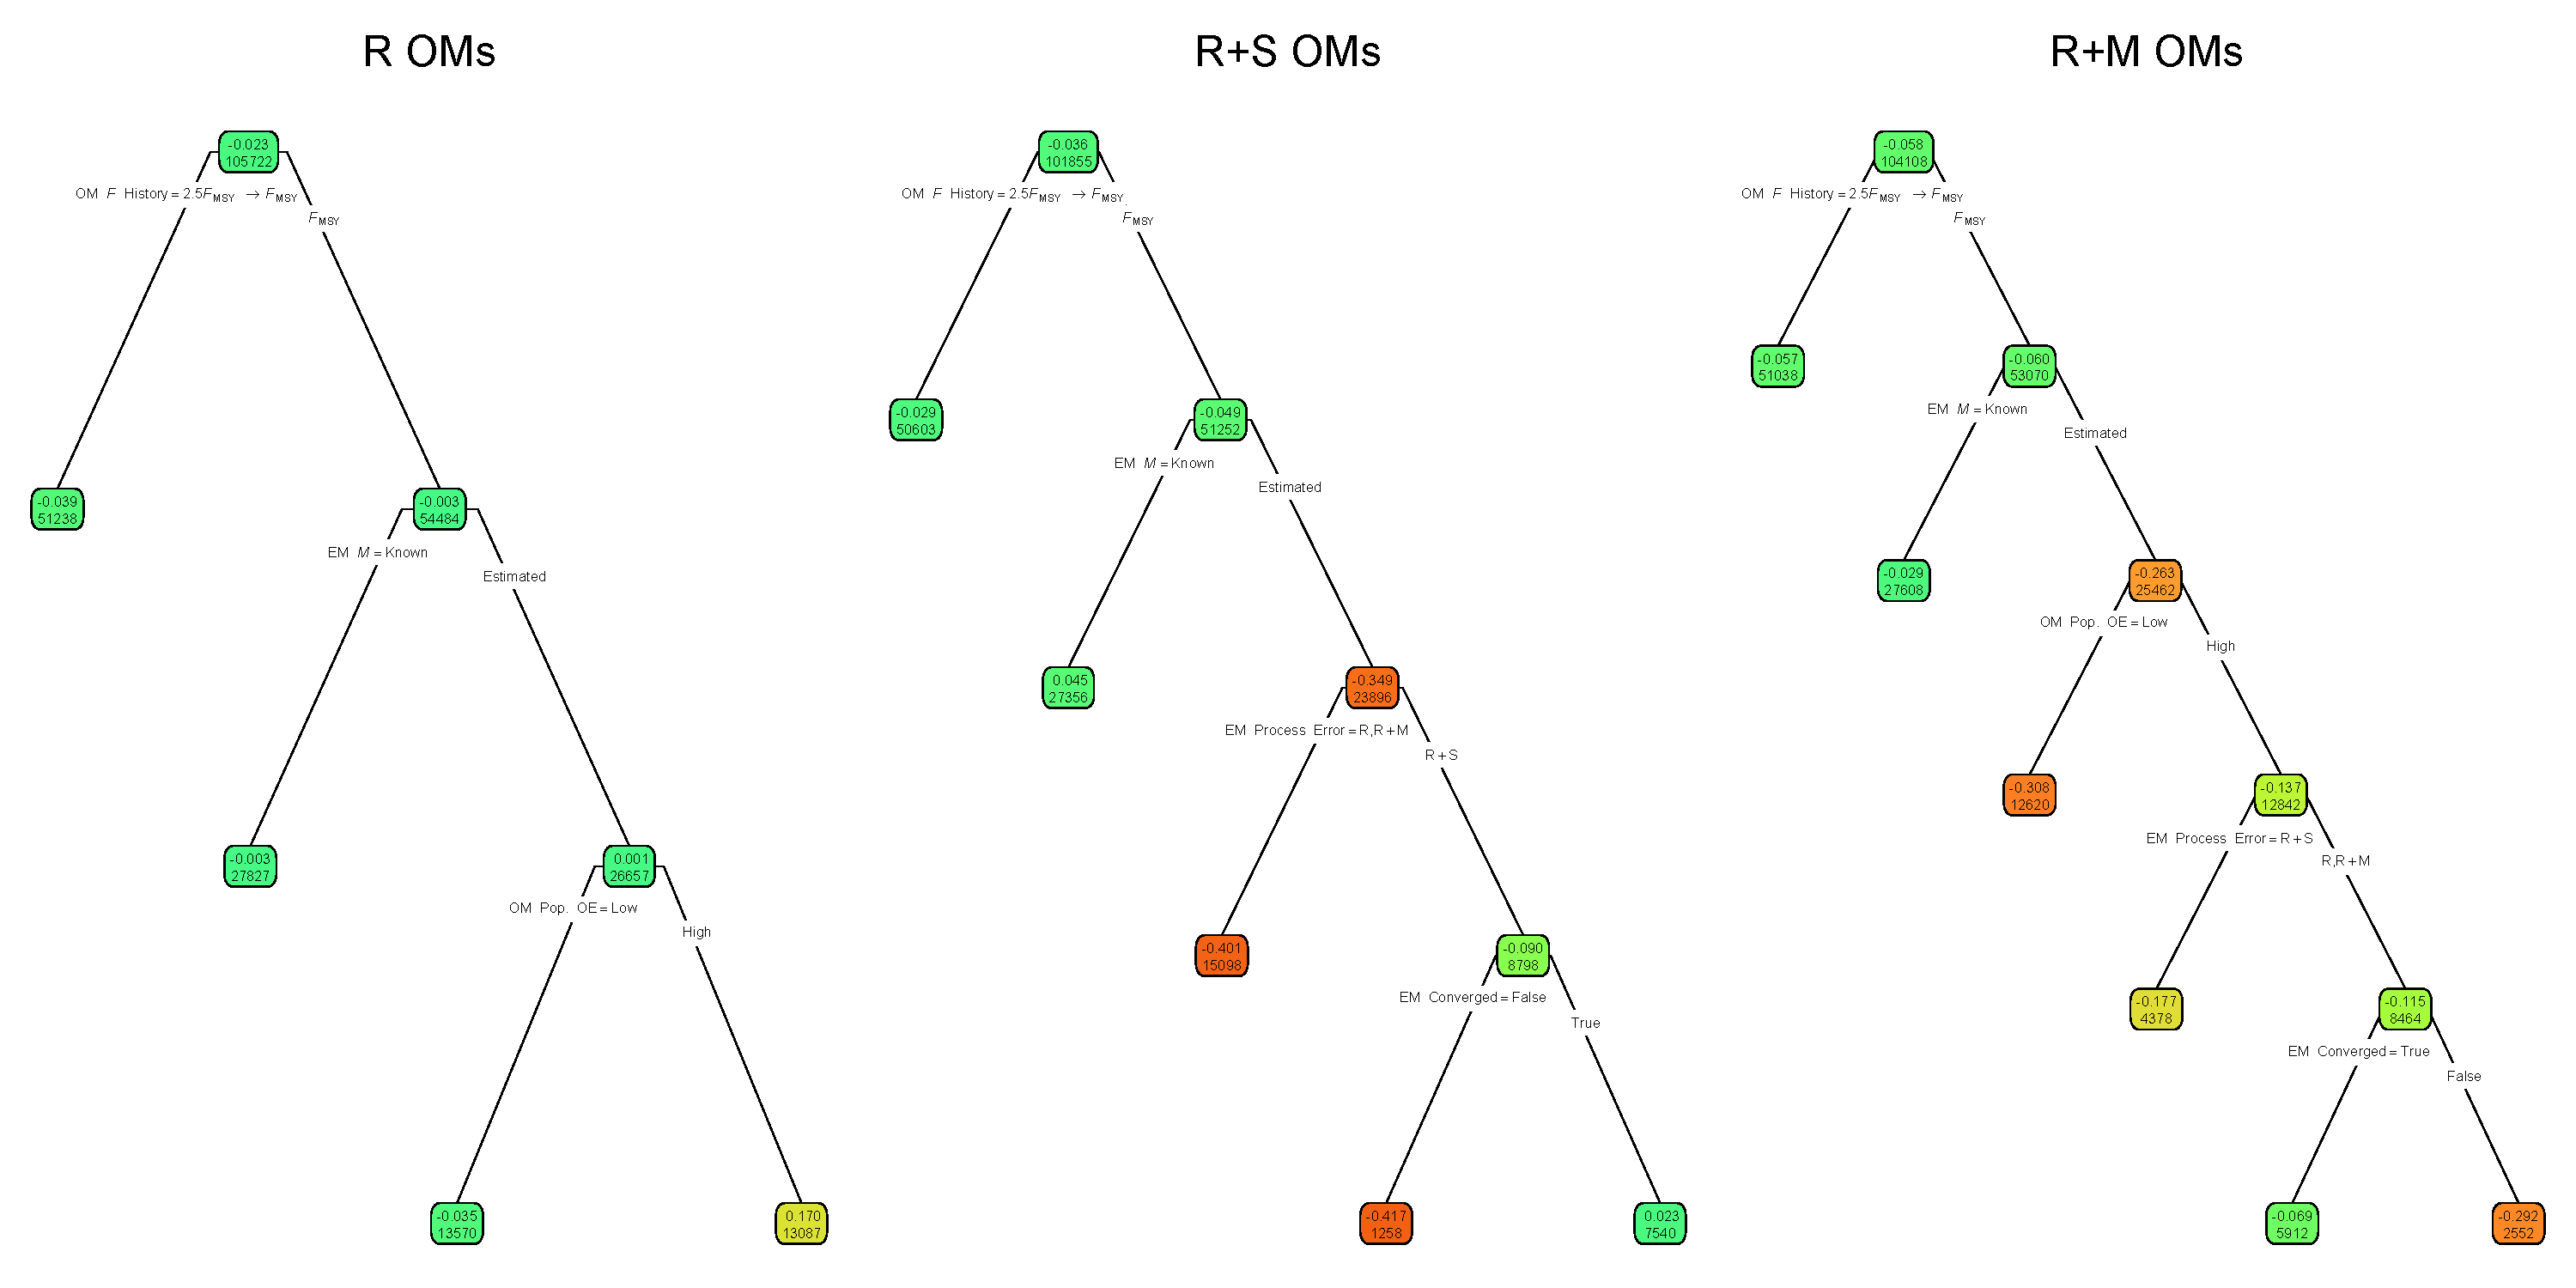
\includegraphics[width = 1.4\textwidth]{term_SSB_bias_regtree_plots}
\end{center}
\caption{Regression trees for estimation error of terminal year SSB as measured by Eq. \ref{relerror_trans_response}. Each node shows the median error for the corresponding subset. Lower or higher absolute median errors are indicated by more green or red polygons, respectively. See Figure \ref{conv_class} caption and Table \ref{factor_table} for further details.}\label{term_SSB_bias_regtree}
\end{figure}
\end{landscape}

\pagebreak

\setcounter{figure}{0}
\renewcommand\thefigure{S\arabic{figure}}

\setcounter{table}{0}
\renewcommand\thetable{S\arabic{table}}

\begin{landscape}
\end{landscape}

\section*{Supplemental Materials}\label{supplemental-materials}
\addcontentsline{toc}{section}{Supplemental Materials}

\subsection*{Referenced Figures and
Tables}\label{referenced-figures-and-tables}
\addcontentsline{toc}{subsection}{Referenced Figures and Tables}

\begin{landscape}
\begin{figure}
\begin{center}
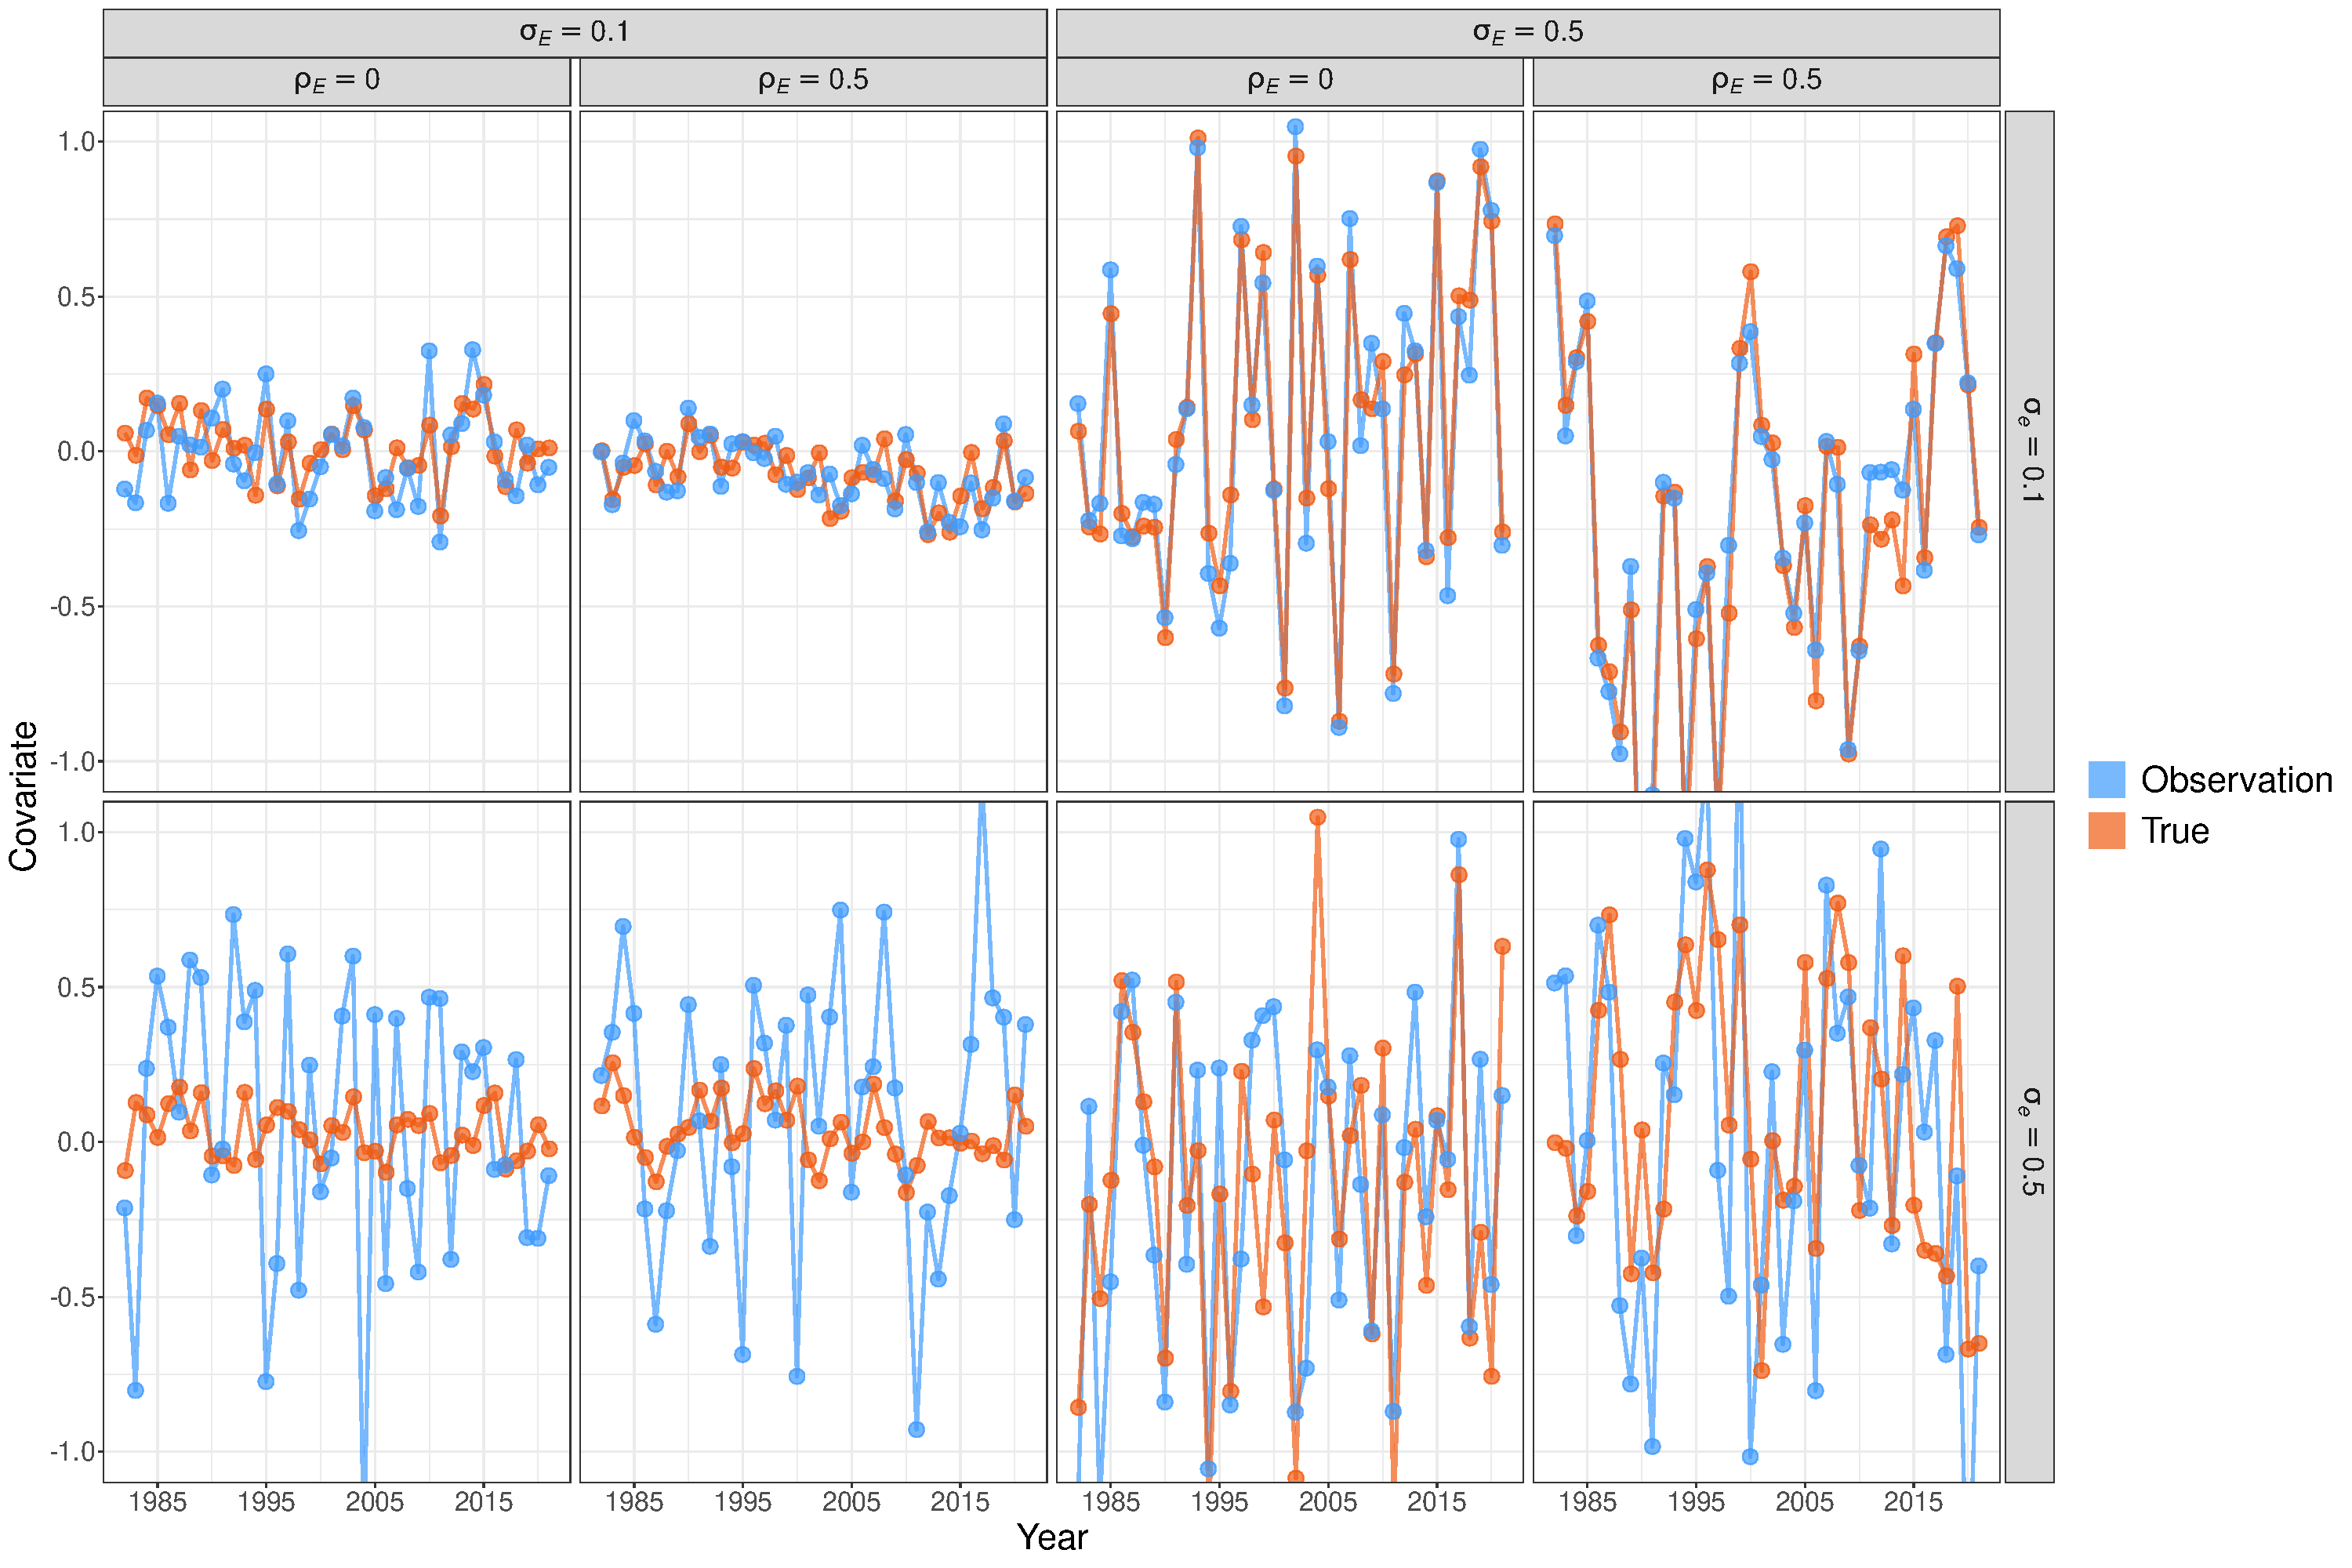
\includegraphics[height = \textheight]{Ecov_true_obs_example}
\end{center}
\caption{Example simulations of environmental covariate latent processes and observations with different levels of observation error, and different assumptions about variability of the latent process.}\label{om_ecov_example}
\end{figure}
\end{landscape}

\begin{figure}
\begin{center}
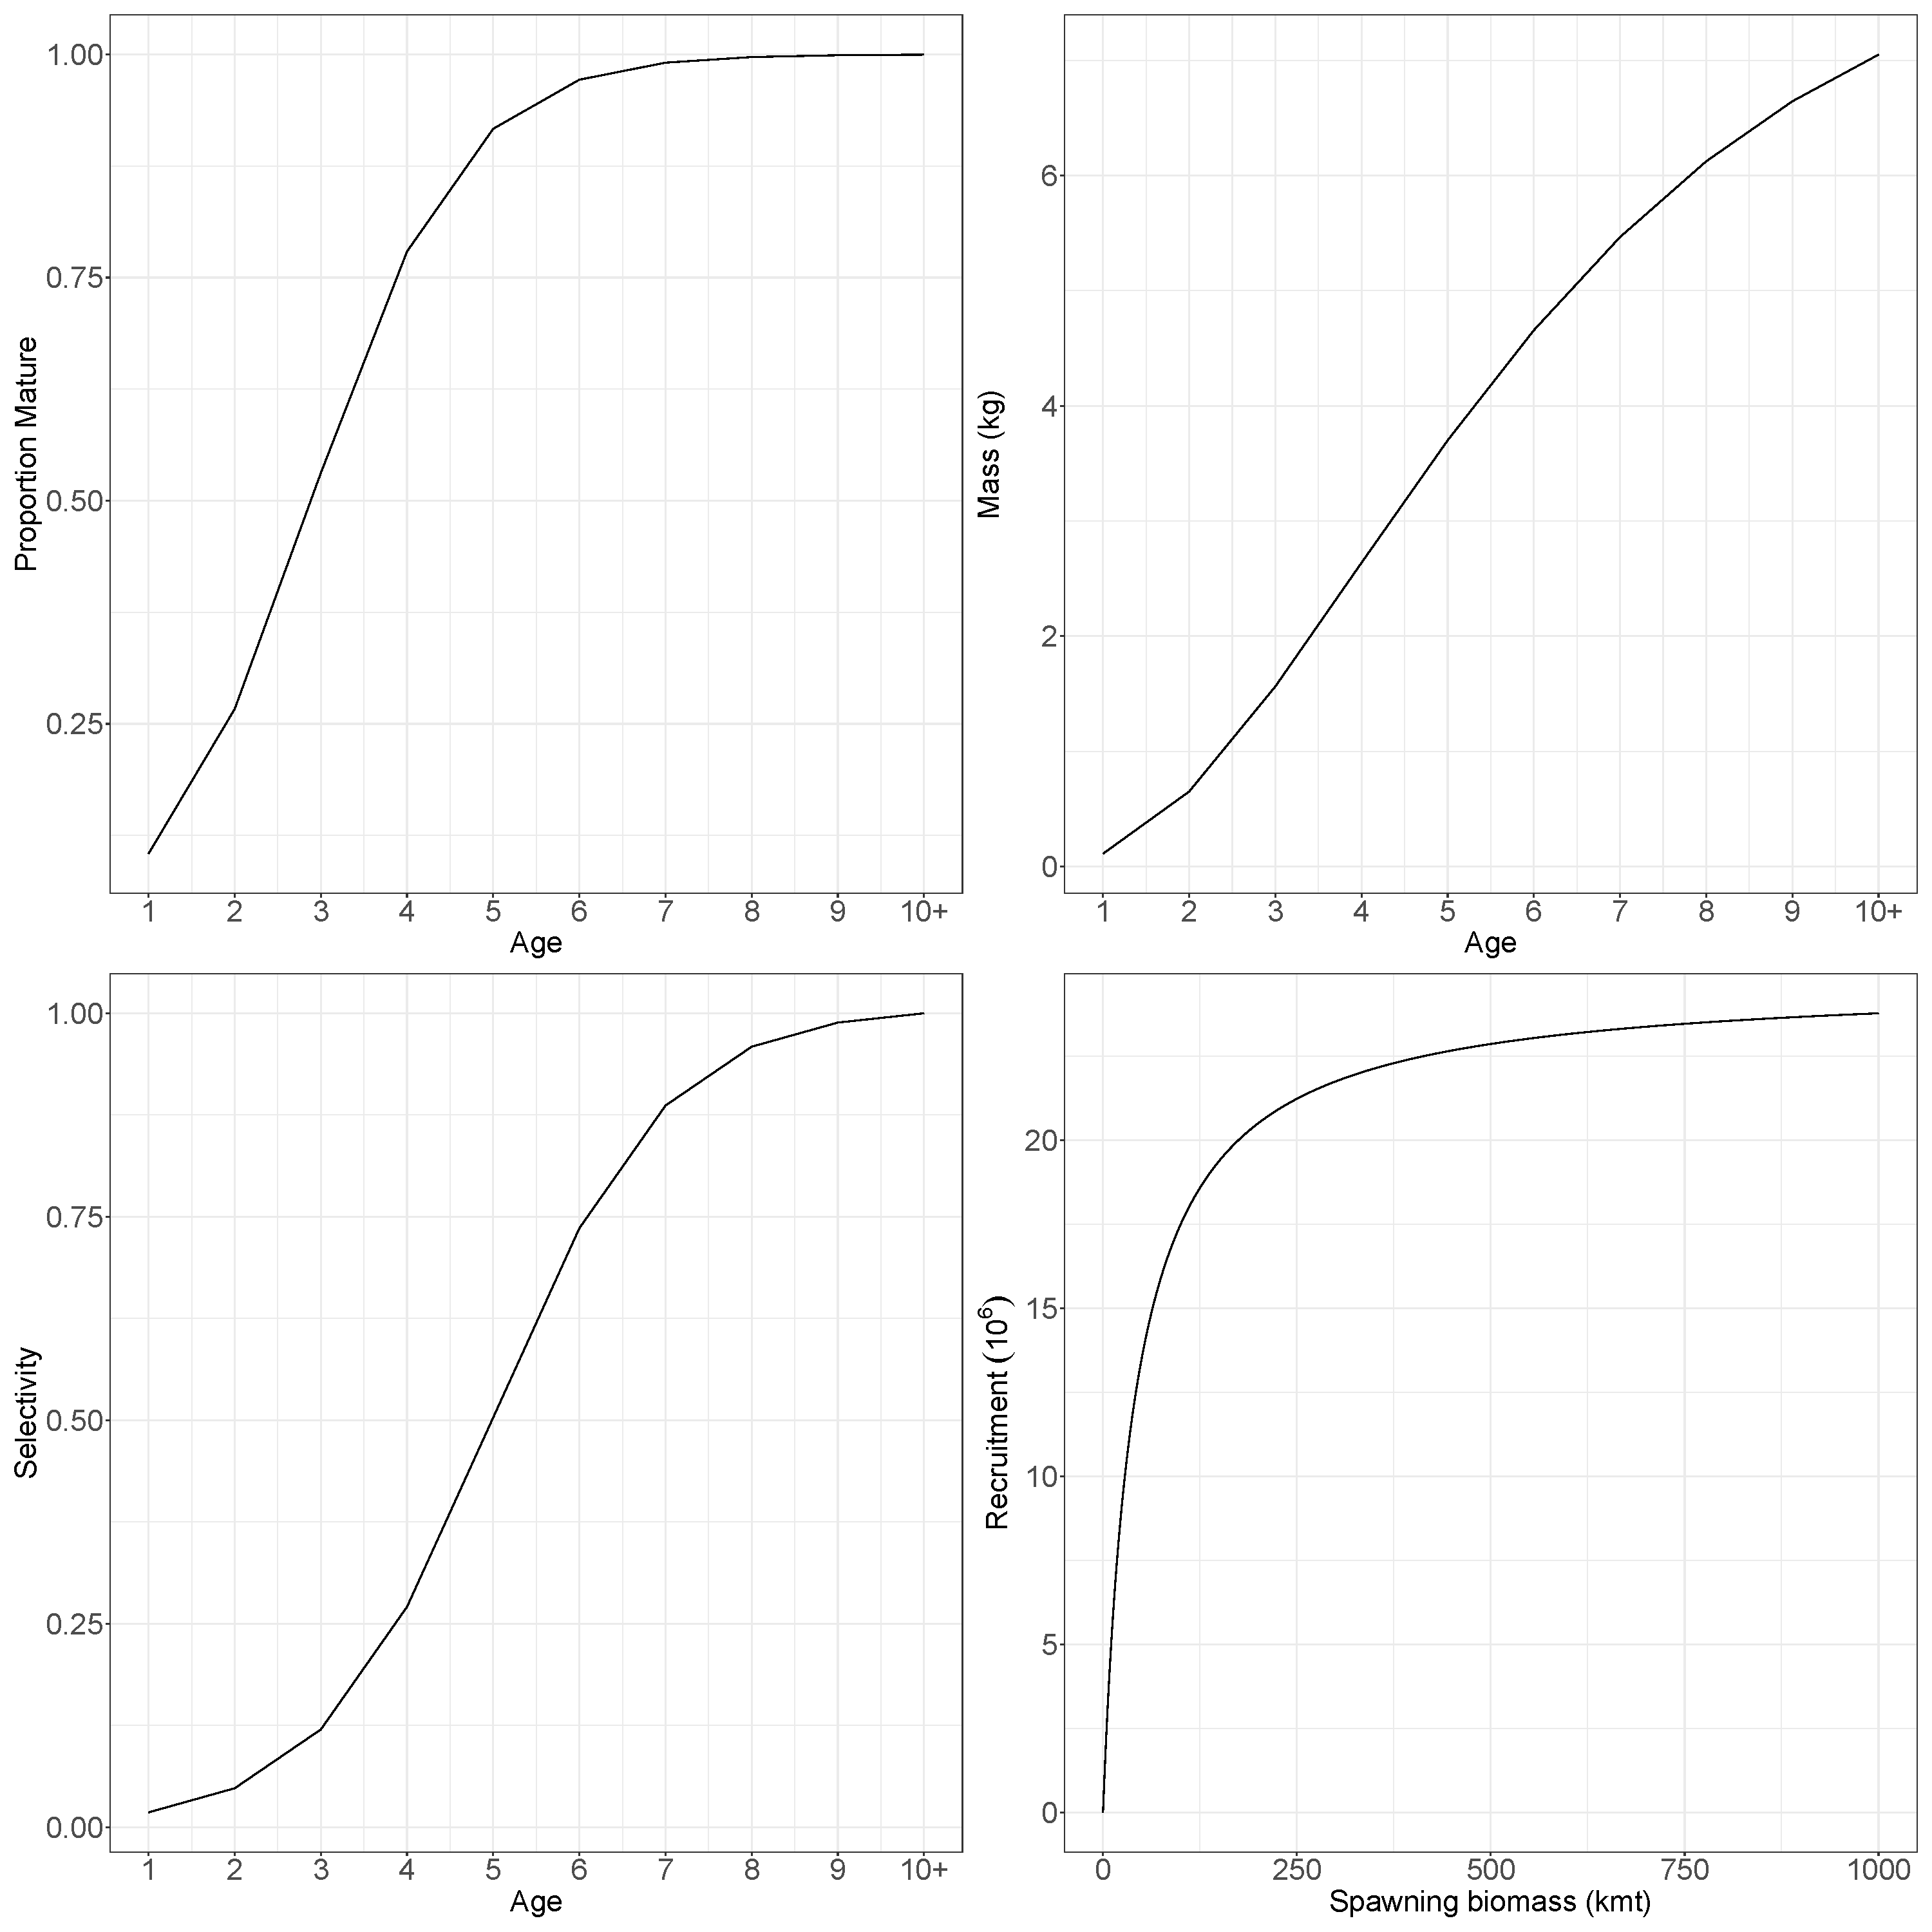
\includegraphics[width = \textwidth]{om_input_plots_figure}
\end{center}
\caption{The proportion mature at age, weight at age, fleet and index selectivity at age, and Beverton-Holt stock-recruit relationship assumed for the population in all operating models. For operating models with random effects on fleet selectivity, this represents the selectivity at the mean of the random effects.}\label{om_inputs_fig}
\end{figure}

\begin{landscape}
\begin{figure}
\begin{center}
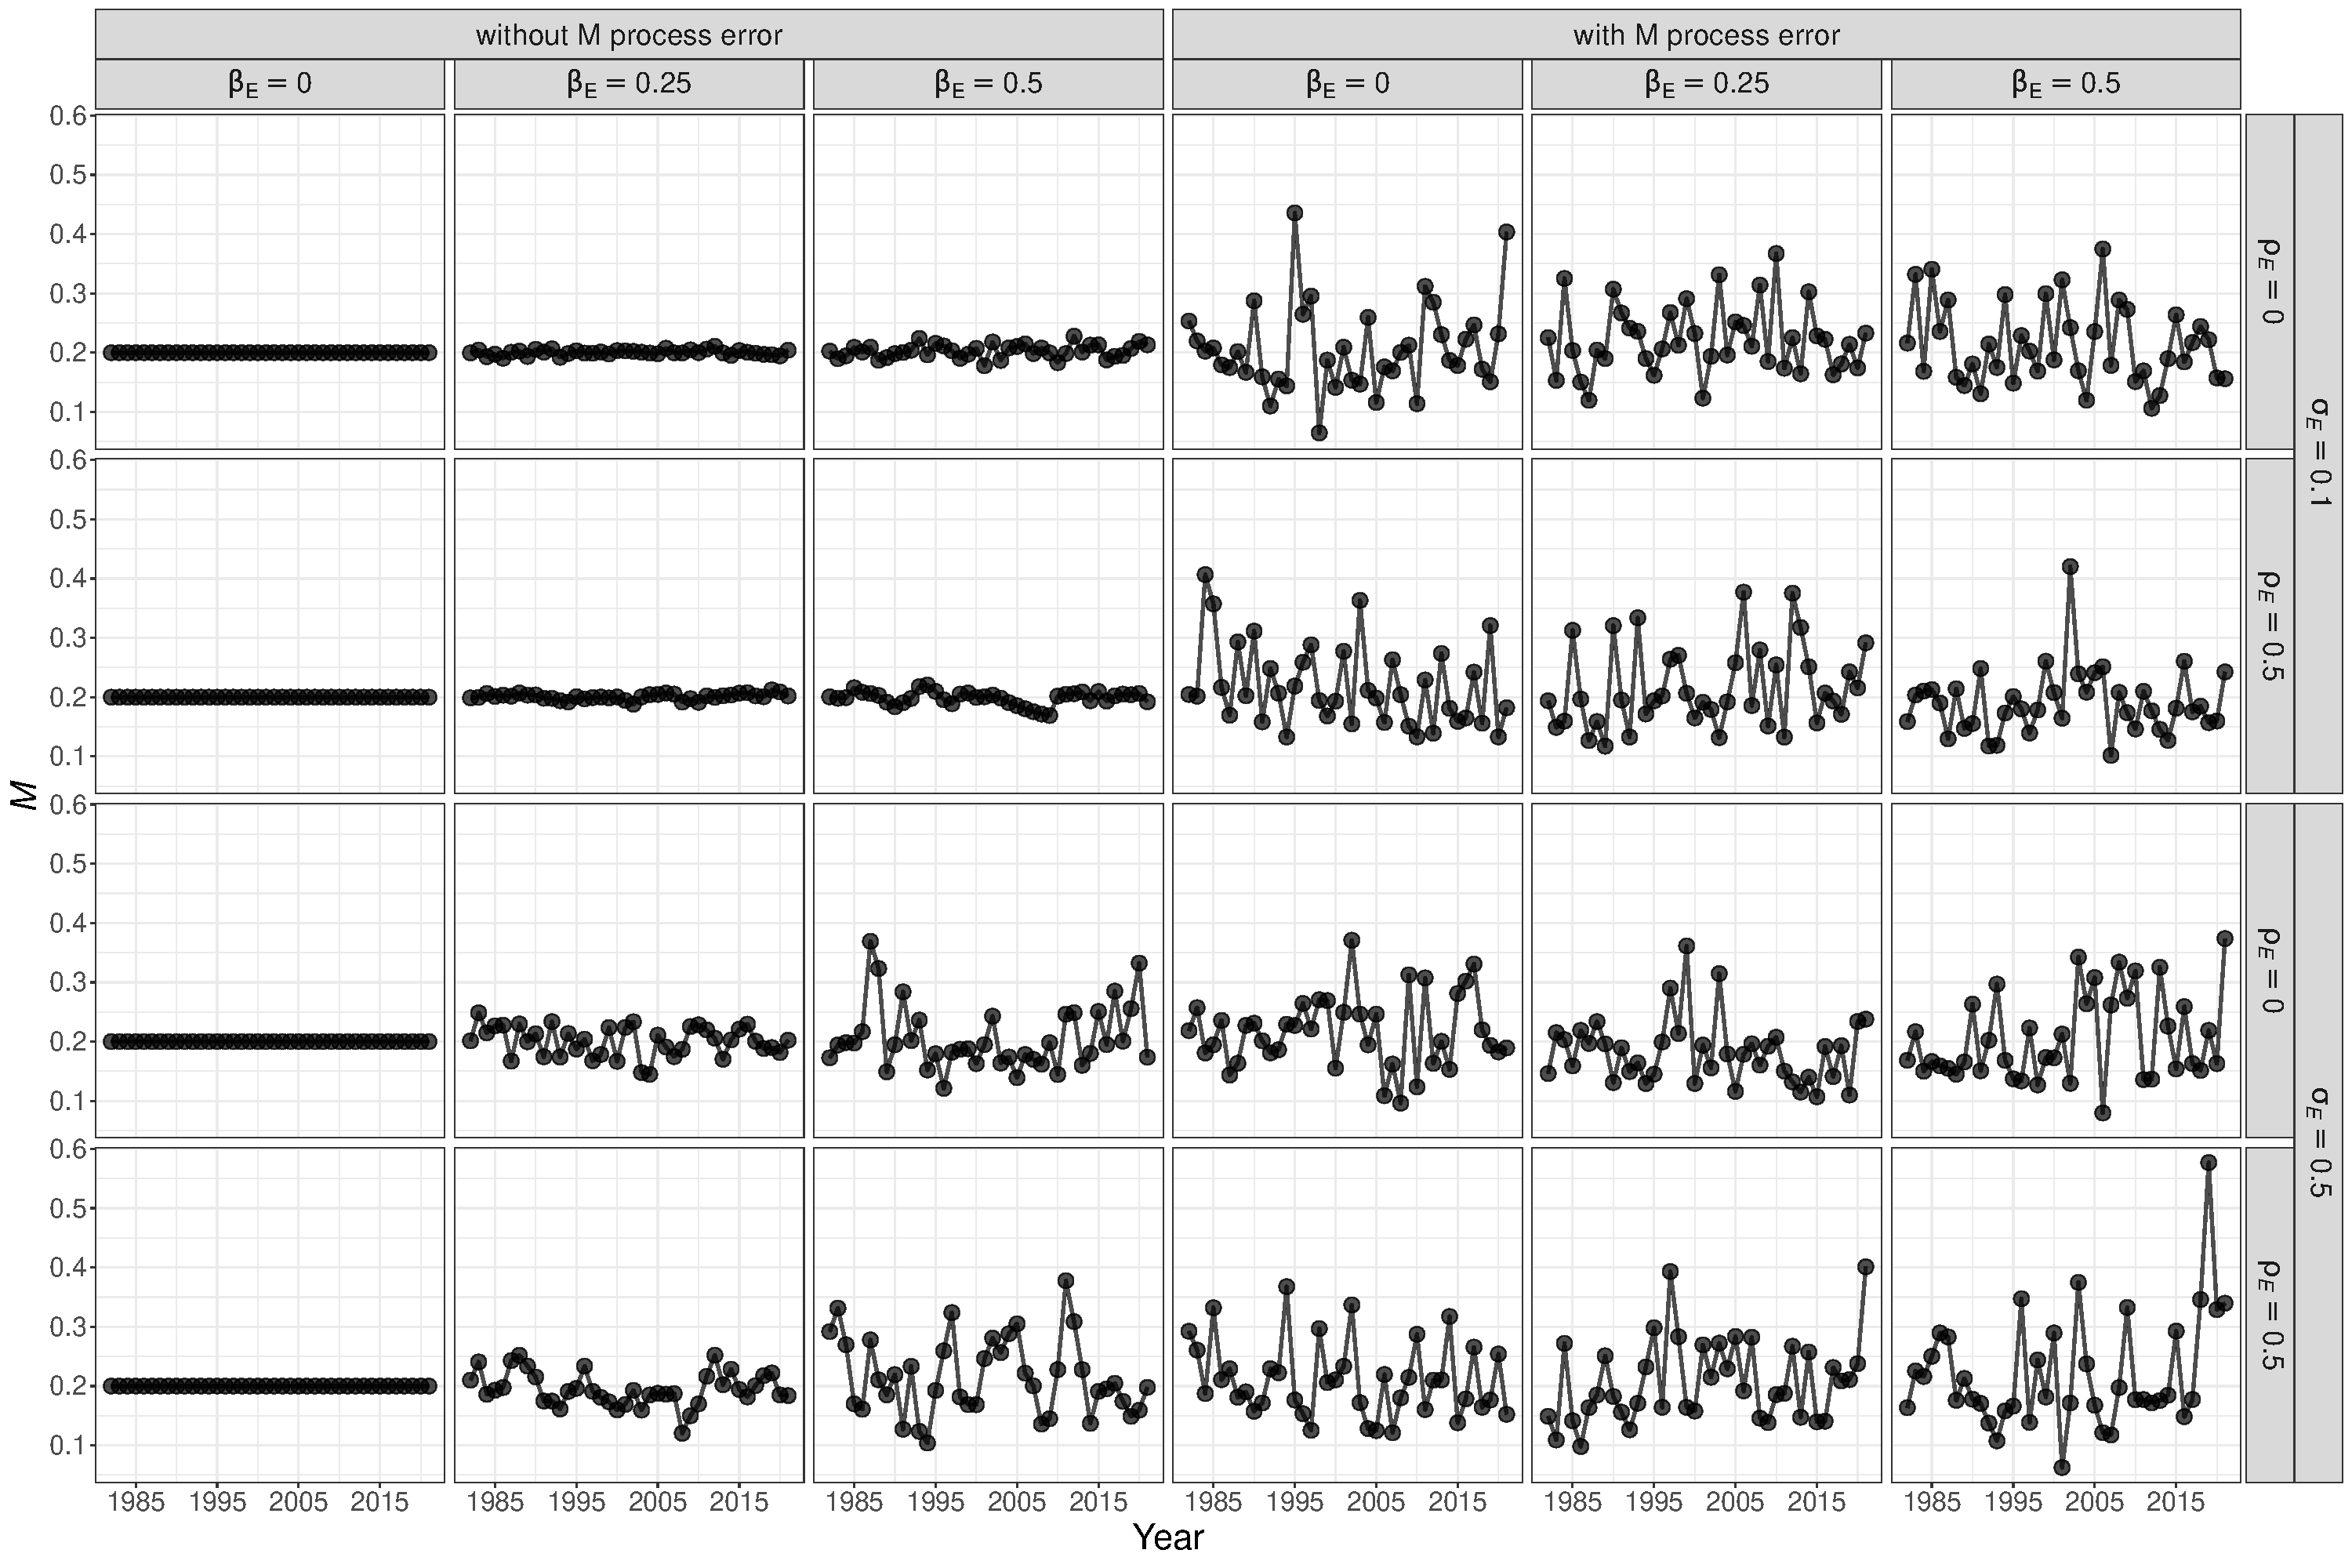
\includegraphics[height = \textheight]{M_example}
\end{center}
\caption{Example simulations of annual $M$ that may be a function of a temporally varying environmental covariate and autoregressive random effects. The marginal standard devation of random effects is $\sigma_M = 0.3$.}\label{M_example}
\end{figure}
\end{landscape}

\begin{landscape}
\begin{figure}
\begin{center}
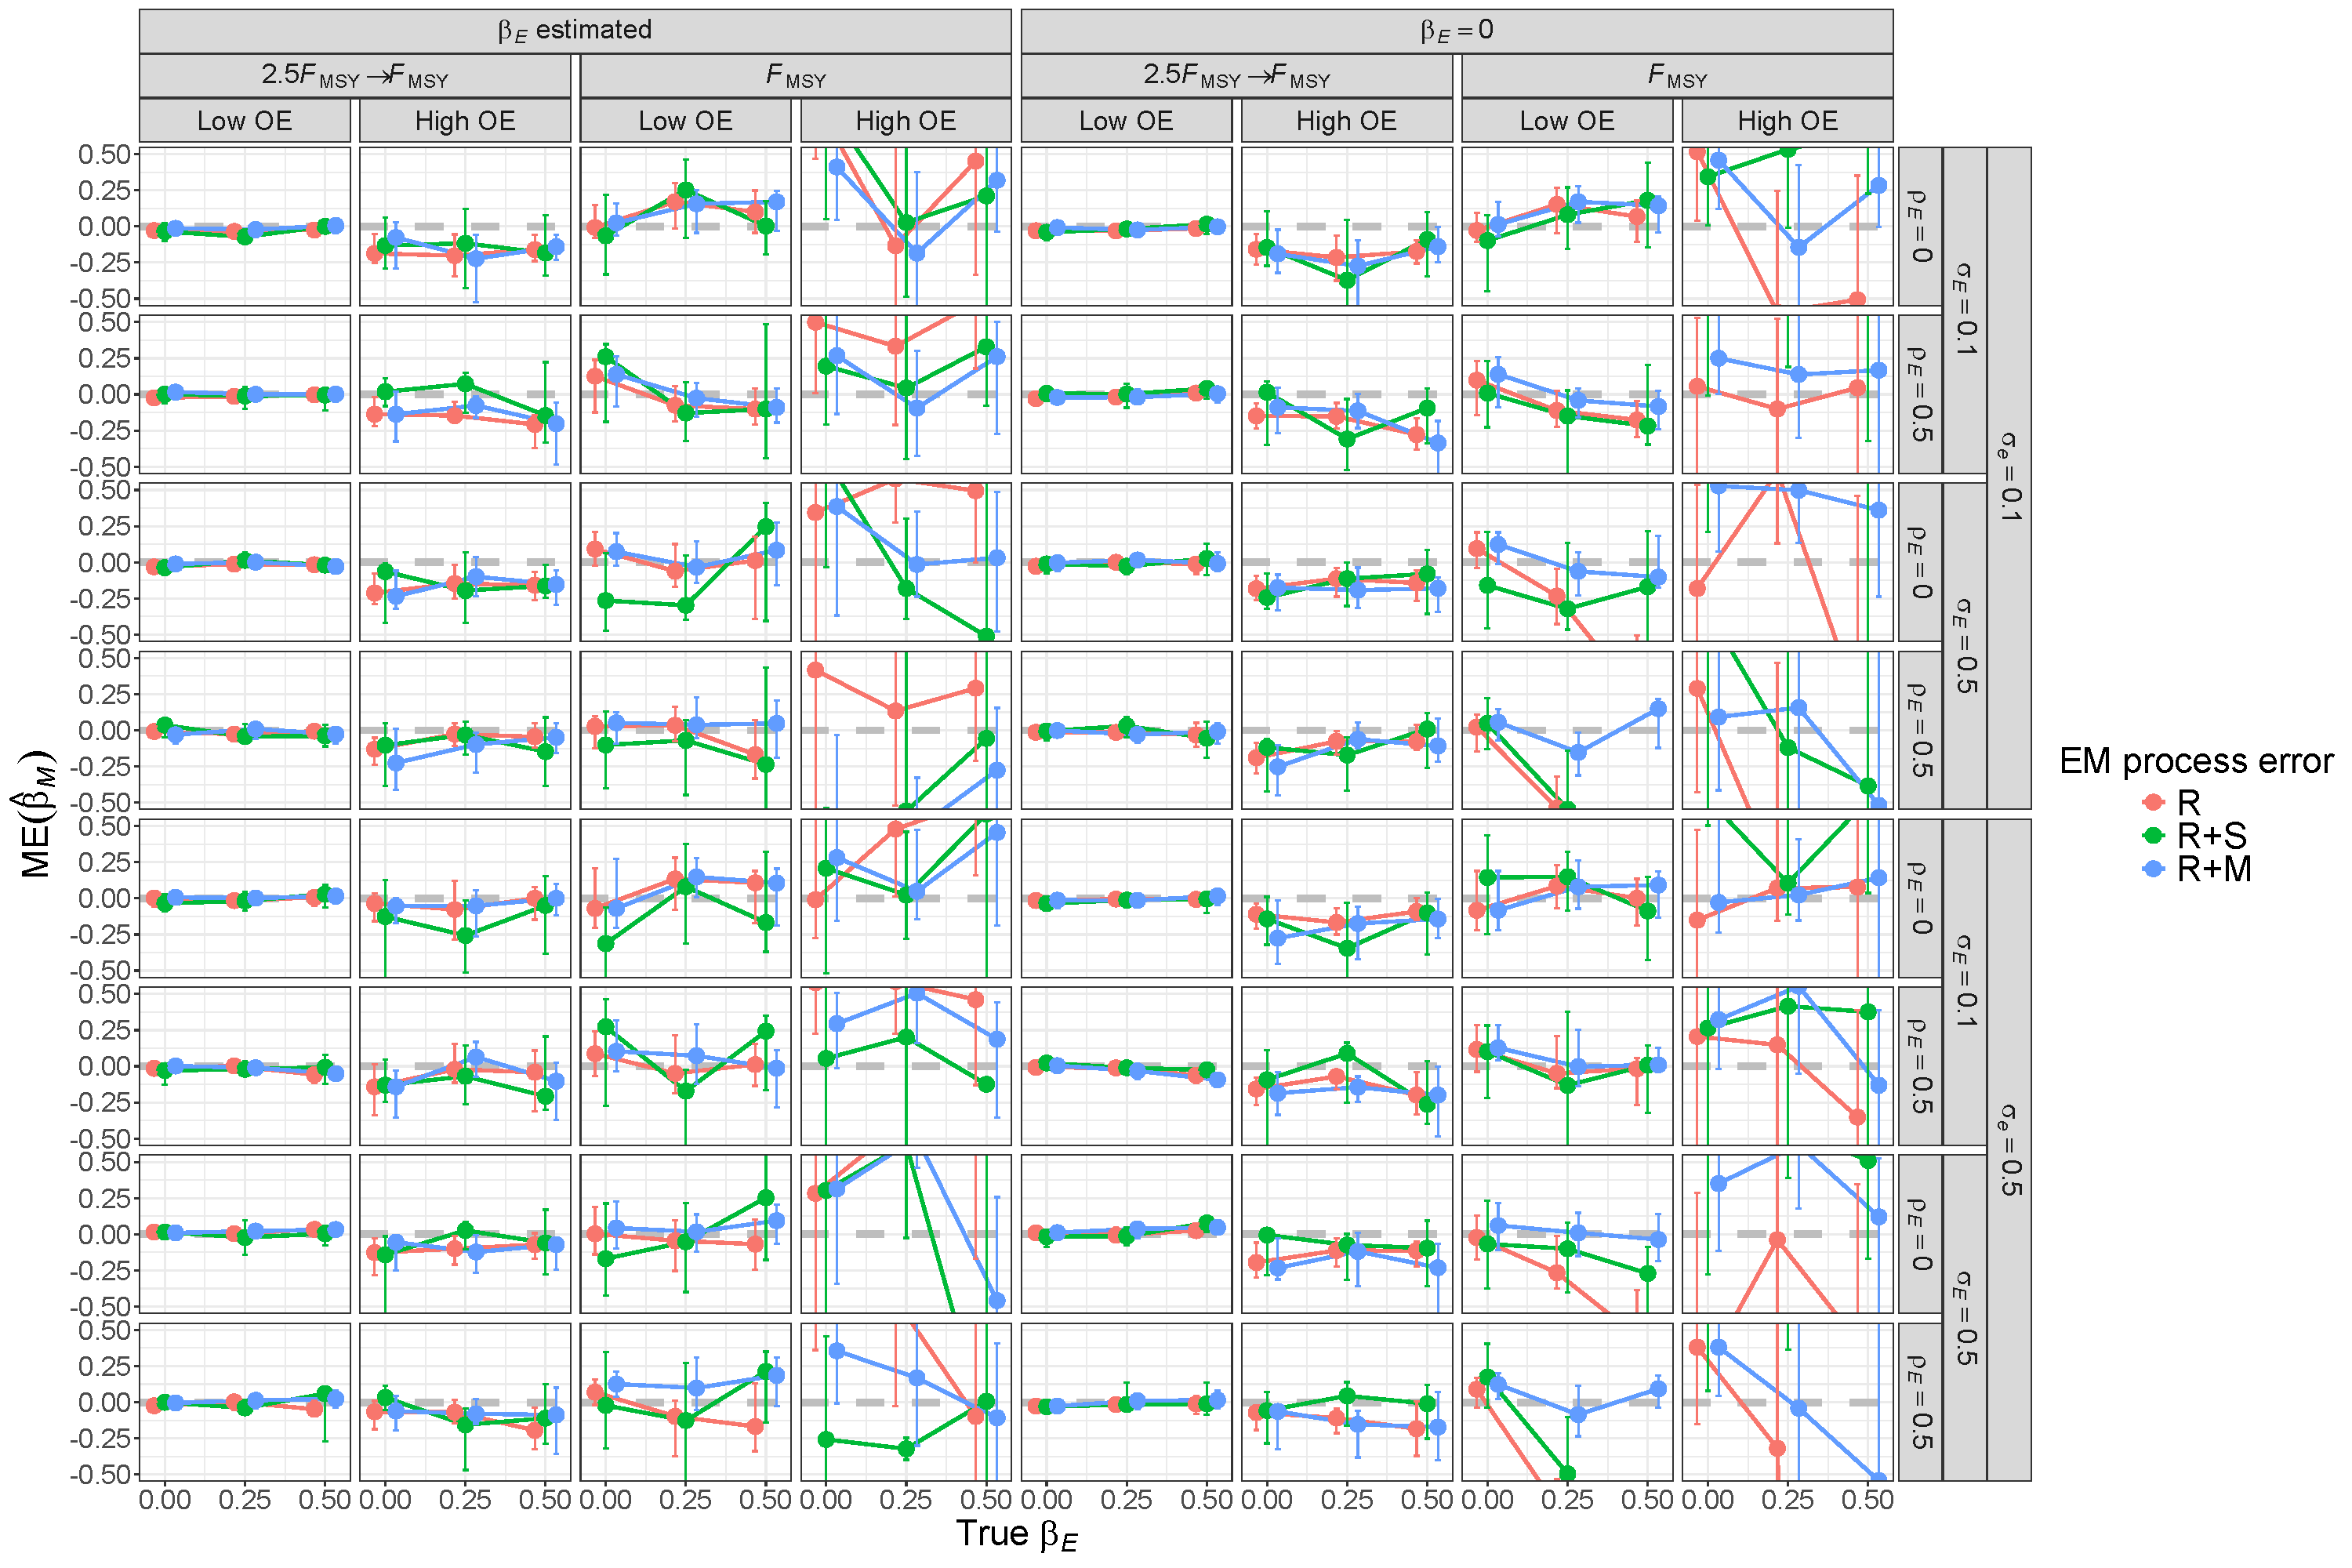
\includegraphics[height = \textheight]{beta_M_bias_Rom}
\end{center}
\caption{For R operating models, median error (ME) of estimates of $\beta_M$ from fitting estimating models with alternative process error assumptions and treatment of covariate effect ($\beta_E = 0$ or estimated). Vertical lines represent 95\% confidence intervals.}\label{beta_M_bias_Rom}
\end{figure}
\end{landscape}

\begin{landscape}
\begin{figure}
\begin{center}
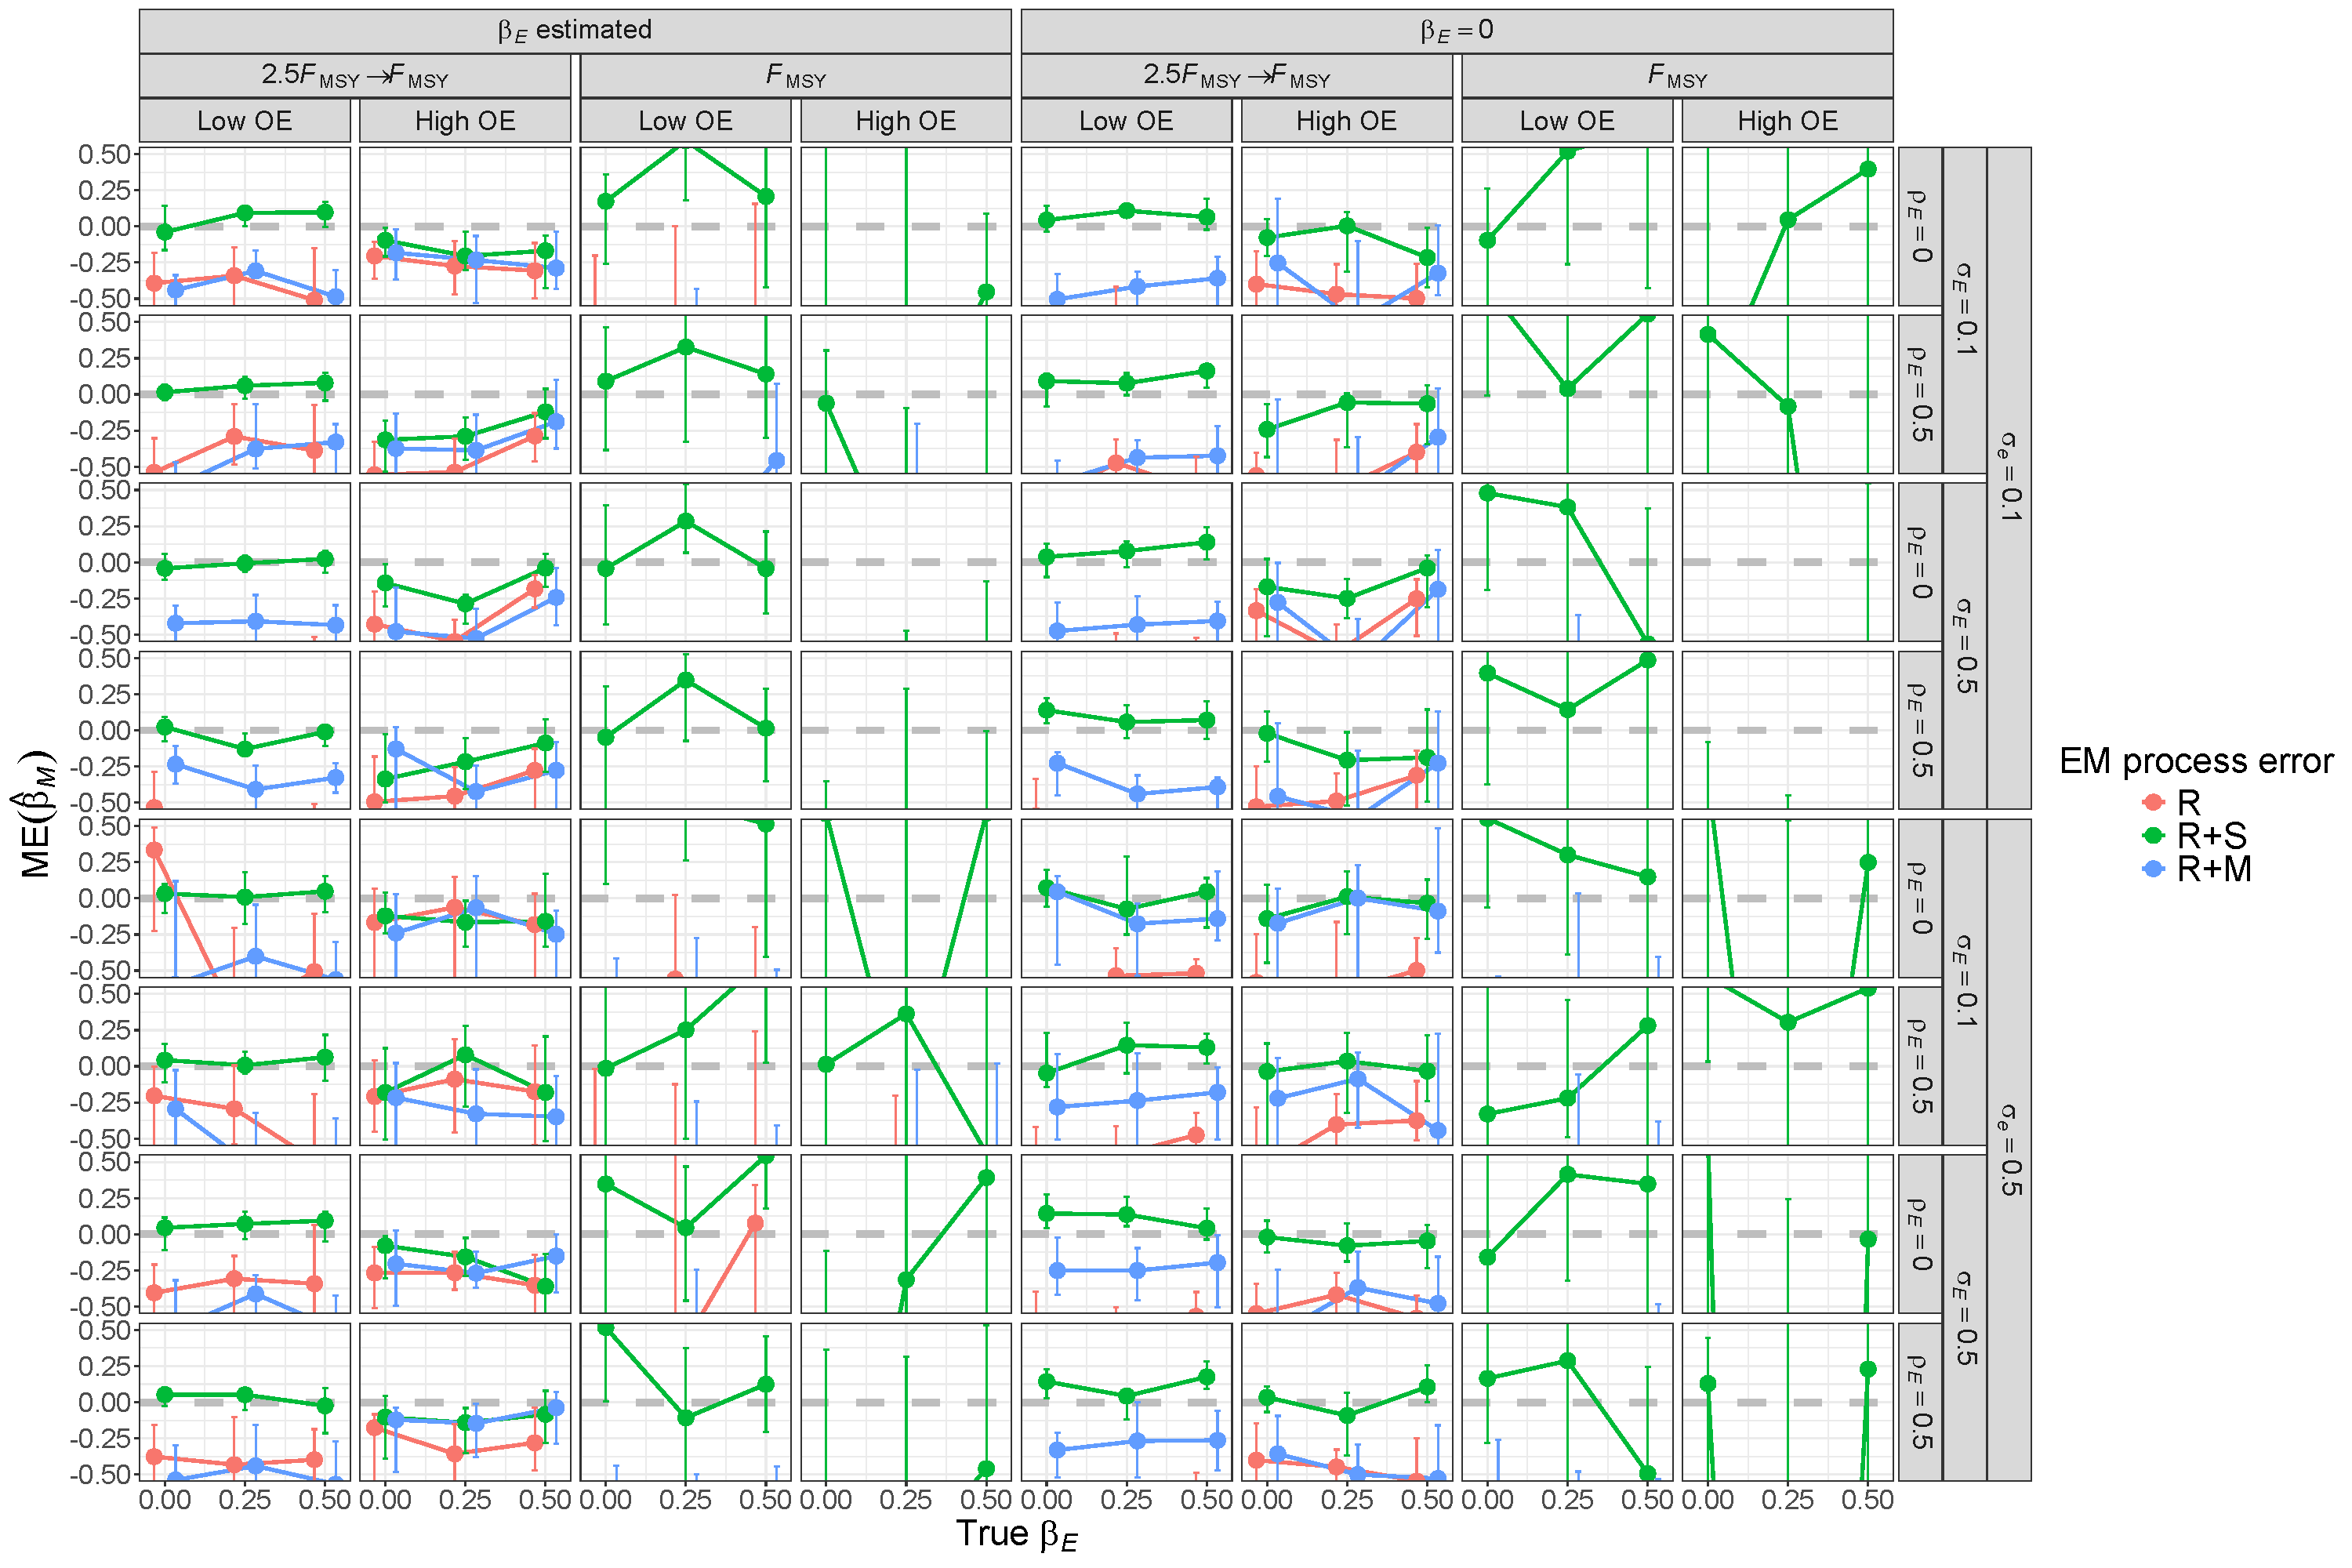
\includegraphics[height = \textheight]{beta_M_bias_RSom}
\end{center}
\caption{For R+S operating models, median error (ME) of estimates of $\beta_M$ from fitting estimating models with alternative process error assumptions and treatment of covariate effect ($\beta_E = 0$ or estimated). Vertical lines represent 95\% confidence intervals.}\label{beta_M_bias_RSom}
\end{figure}
\end{landscape}

\begin{landscape}
\begin{figure}
\begin{center}
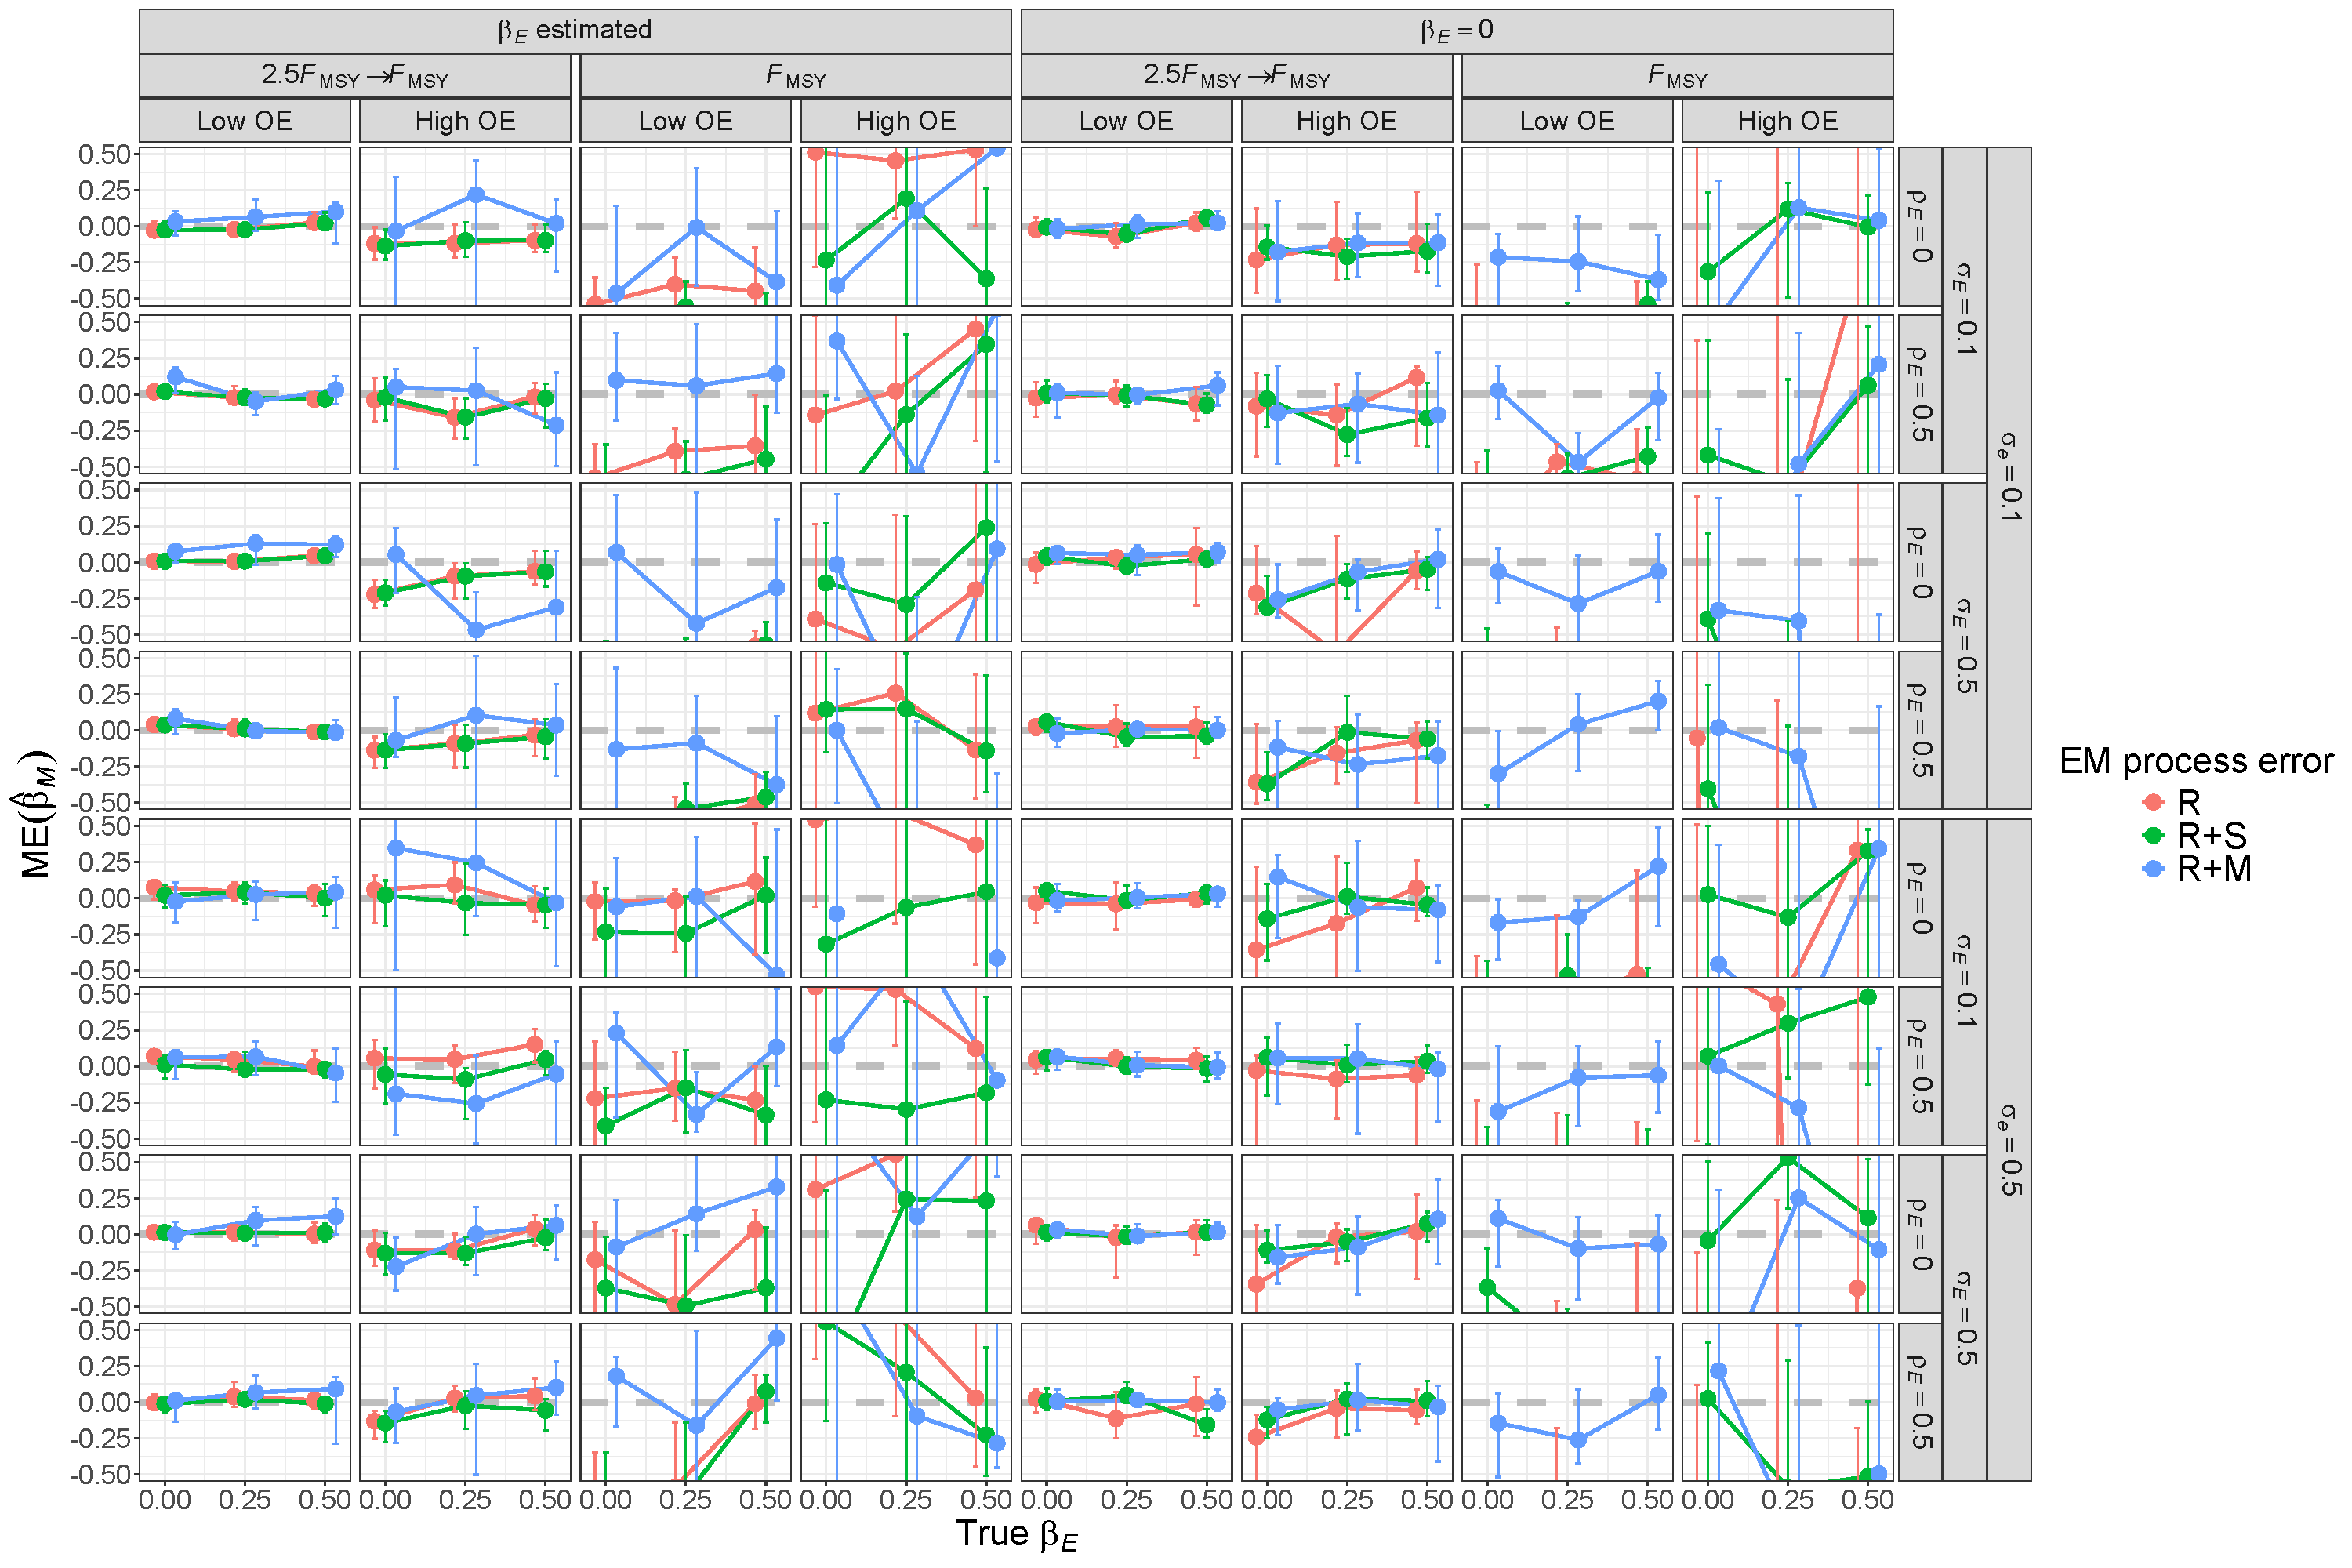
\includegraphics[height = \textheight]{beta_M_bias_RMom}
\end{center}
\caption{For R+M operating models, median error (ME) of estimates of $\beta_M$ from fitting estimating models with alternative process error assumptions and treatment of covariate effect ($\beta_E = 0$ or estimated). Vertical lines represent 95\% confidence intervals.}\label{beta_M_bias_RMom}
\end{figure}
\end{landscape}

\begin{landscape}
\begin{figure}
\begin{center}
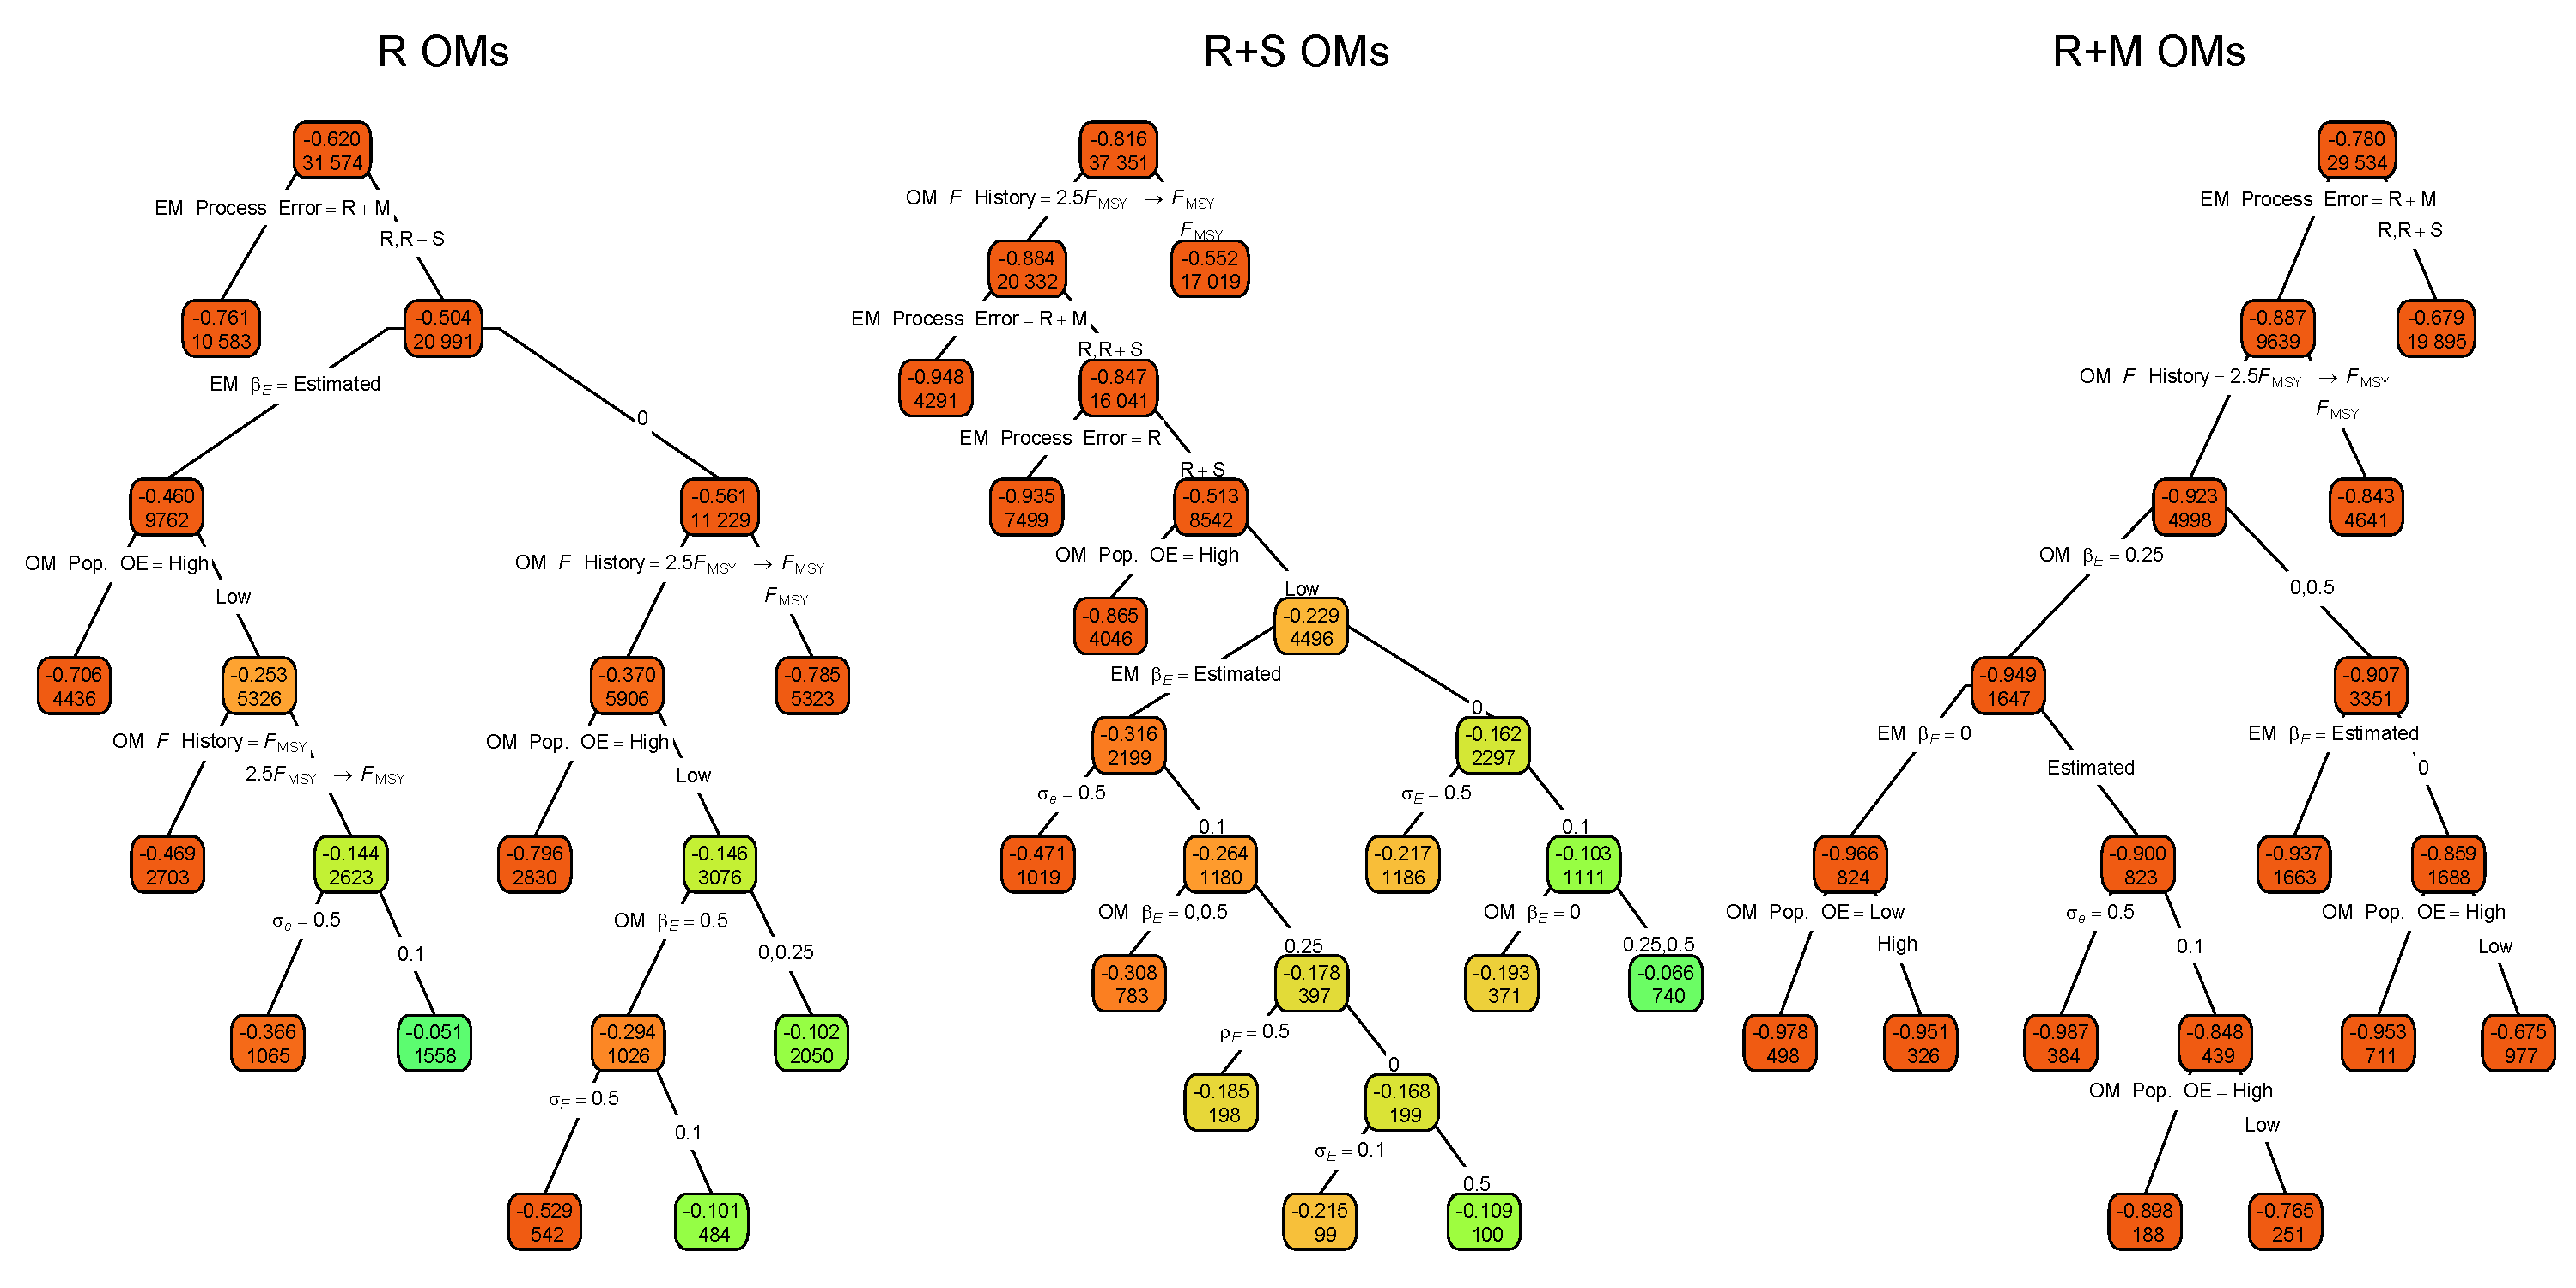
\includegraphics[width = 1.4\textwidth]{median_M_SE_bias_regtree_plots}
\end{center}
\caption{Regression trees for errors of the Hessian-based standard error estimates for median $M$ parameter ($\widehat {\text{SE}}\left(\widehat \beta_M\right)$). Each node shows the median error for the corresponding subset. Lower or higher absolute median absolute errors of the process error assumption are indicated by more green or red polygons, respectively. See Figure \ref{conv_class} caption and Table \ref{factor_table} for further details.}\label{med_M_SE_bias_regtree}
\end{figure}
\end{landscape}

\begin{landscape}
\begin{figure}
\begin{center}
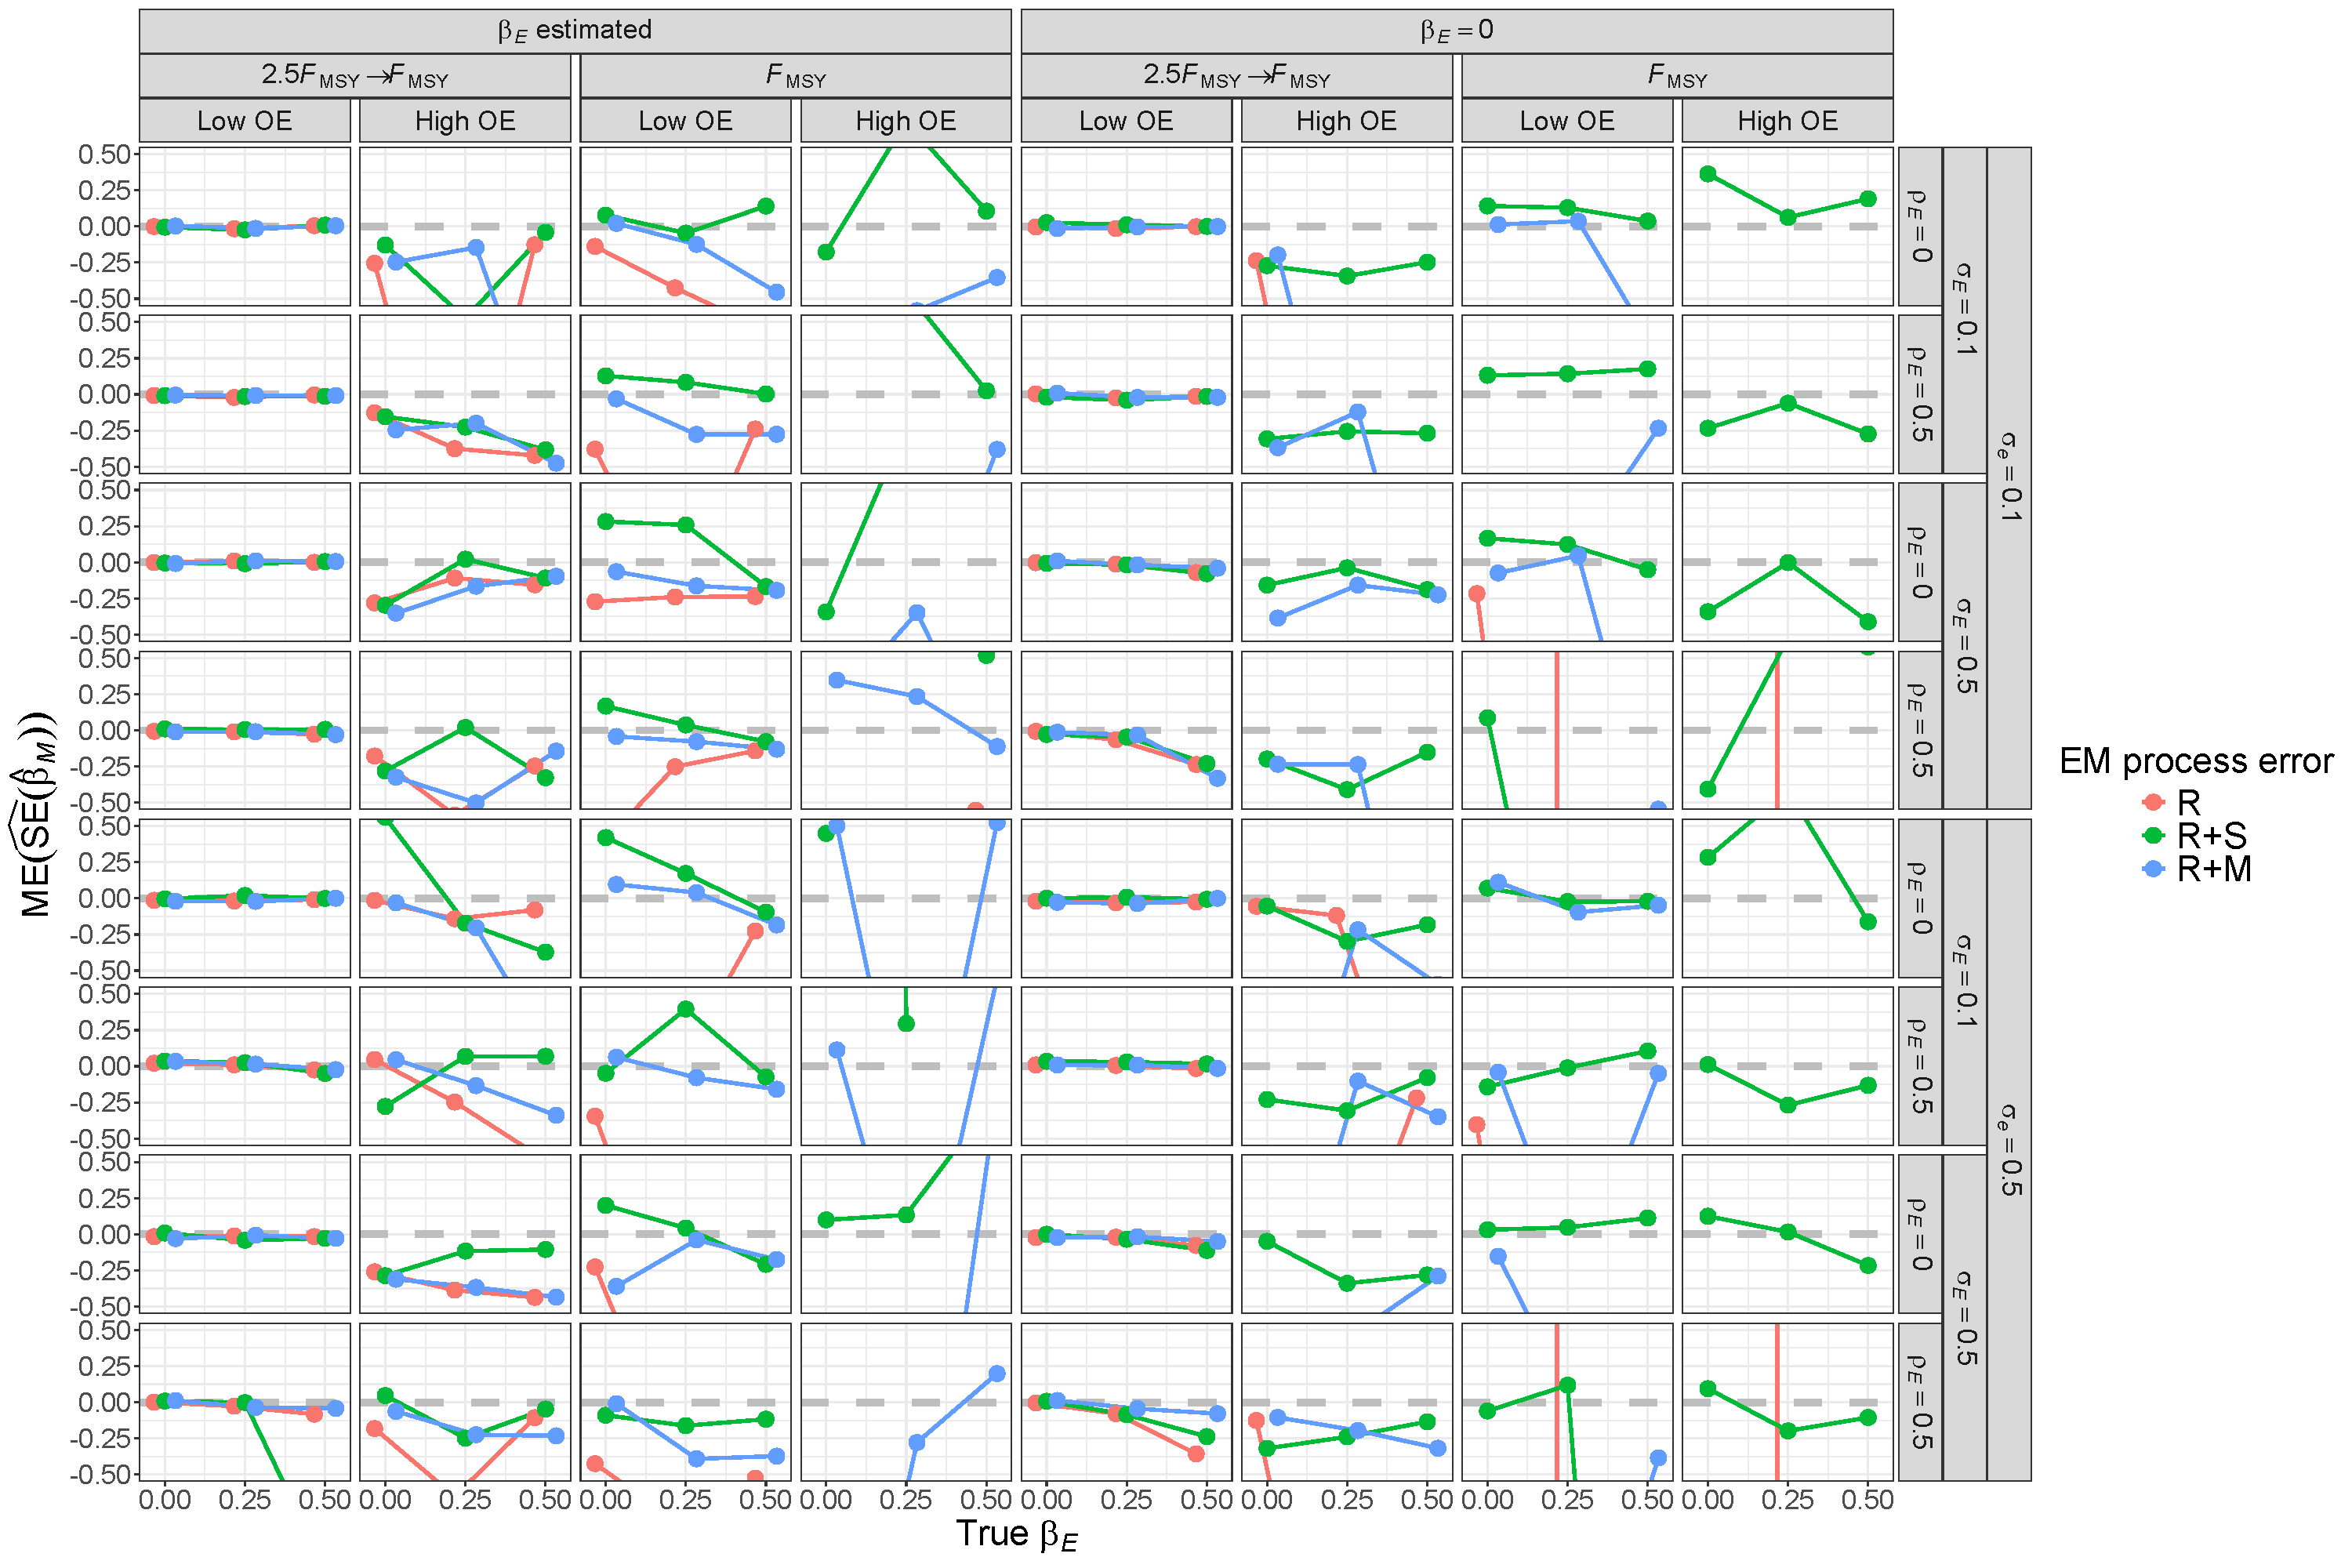
\includegraphics[height = \textheight]{se_beta_M_bias_Rom}
\end{center}
\caption{For R operating models, median error (ME) of Hessian-based estimates of standard error for median $M$ parameter ($\beta_M$) from fitting estimating models with alternative process error assumptions and treatment of the covariate effect ($\beta_ E= 0$ or estimated). True standard error is defined as the mean of the standard error estimates accross converged fits to simulated data sets for a given operating model scenario.}\label{se_beta_M_bias_Rom}
\end{figure}
\end{landscape}

\begin{landscape}
\begin{figure}
\begin{center}
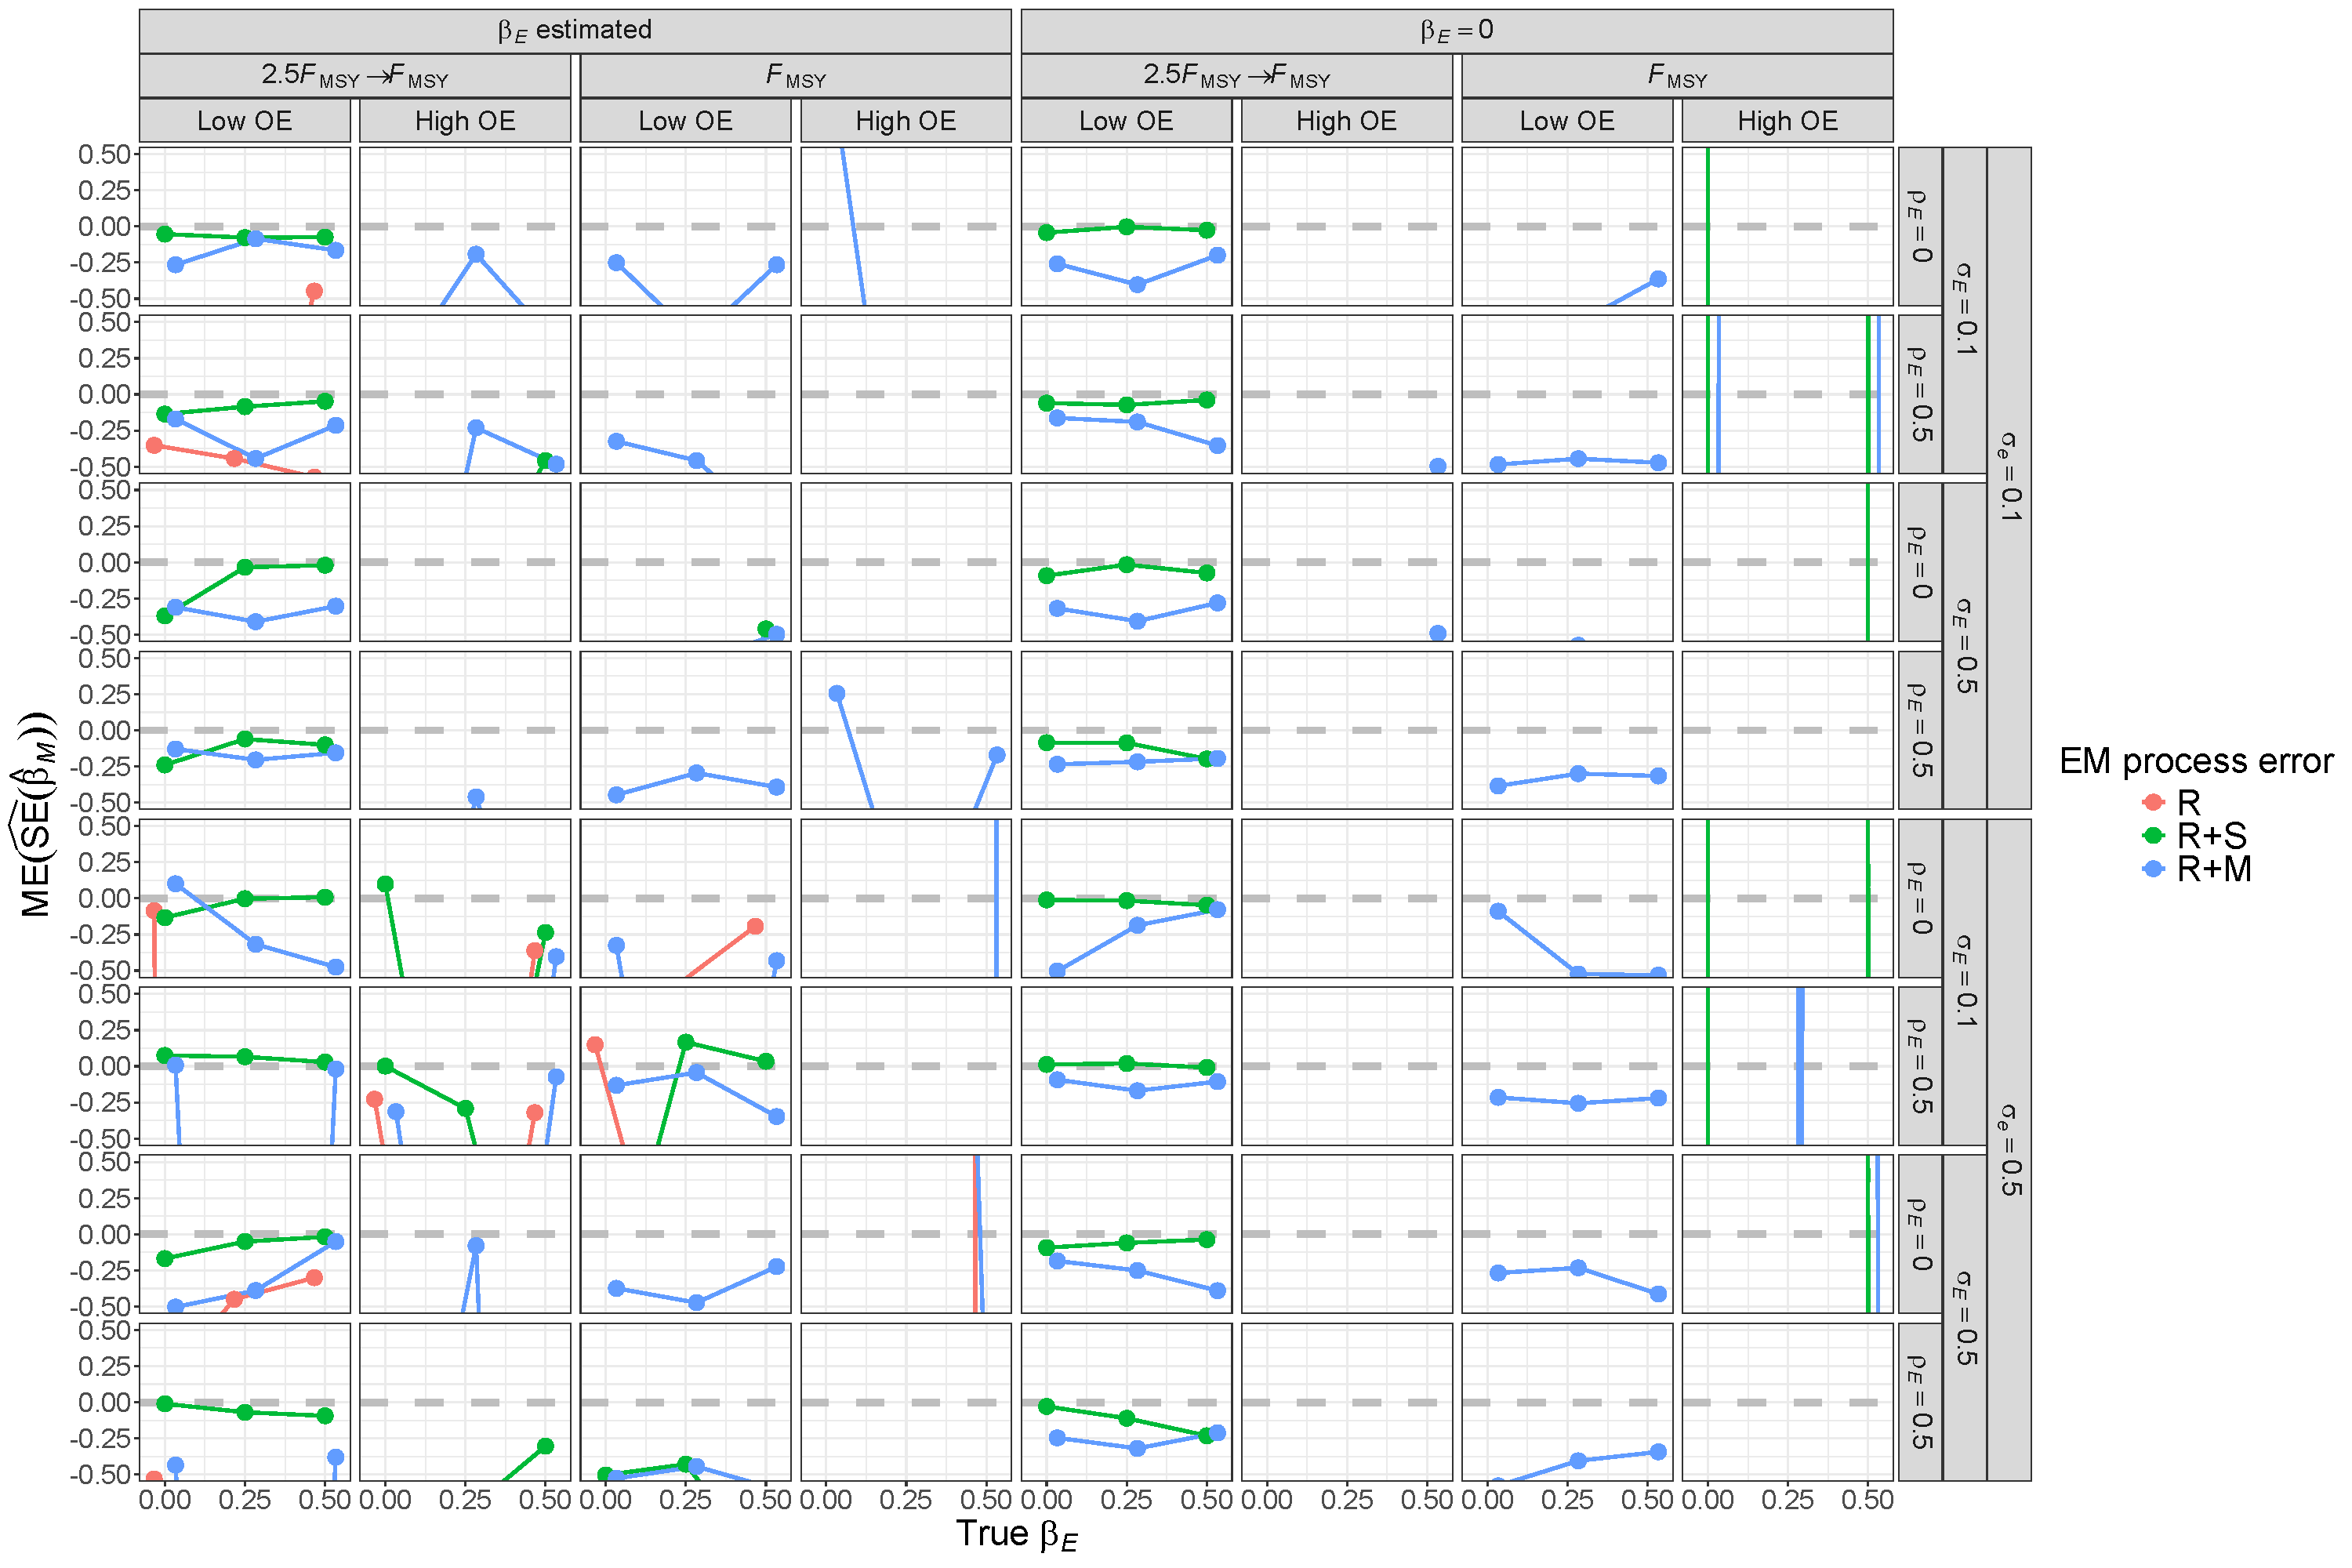
\includegraphics[height = \textheight]{se_beta_M_bias_RSom}
\end{center}
\caption{For R+S operating models, median error (ME) of Hessian-based estimates of standard error for median $M$ parameter ($\beta_M$) from fitting estimating models with alternative process error assumptions and treatment of the covariate effect ($\beta_ E= 0$ or estimated). True standard error is defined as the mean of the standard error estimates accross converged fits to simulated data sets for a given operating model scenario.}\label{se_beta_M_bias_RSom}
\end{figure}
\end{landscape}

\begin{landscape}
\begin{figure}
\begin{center}
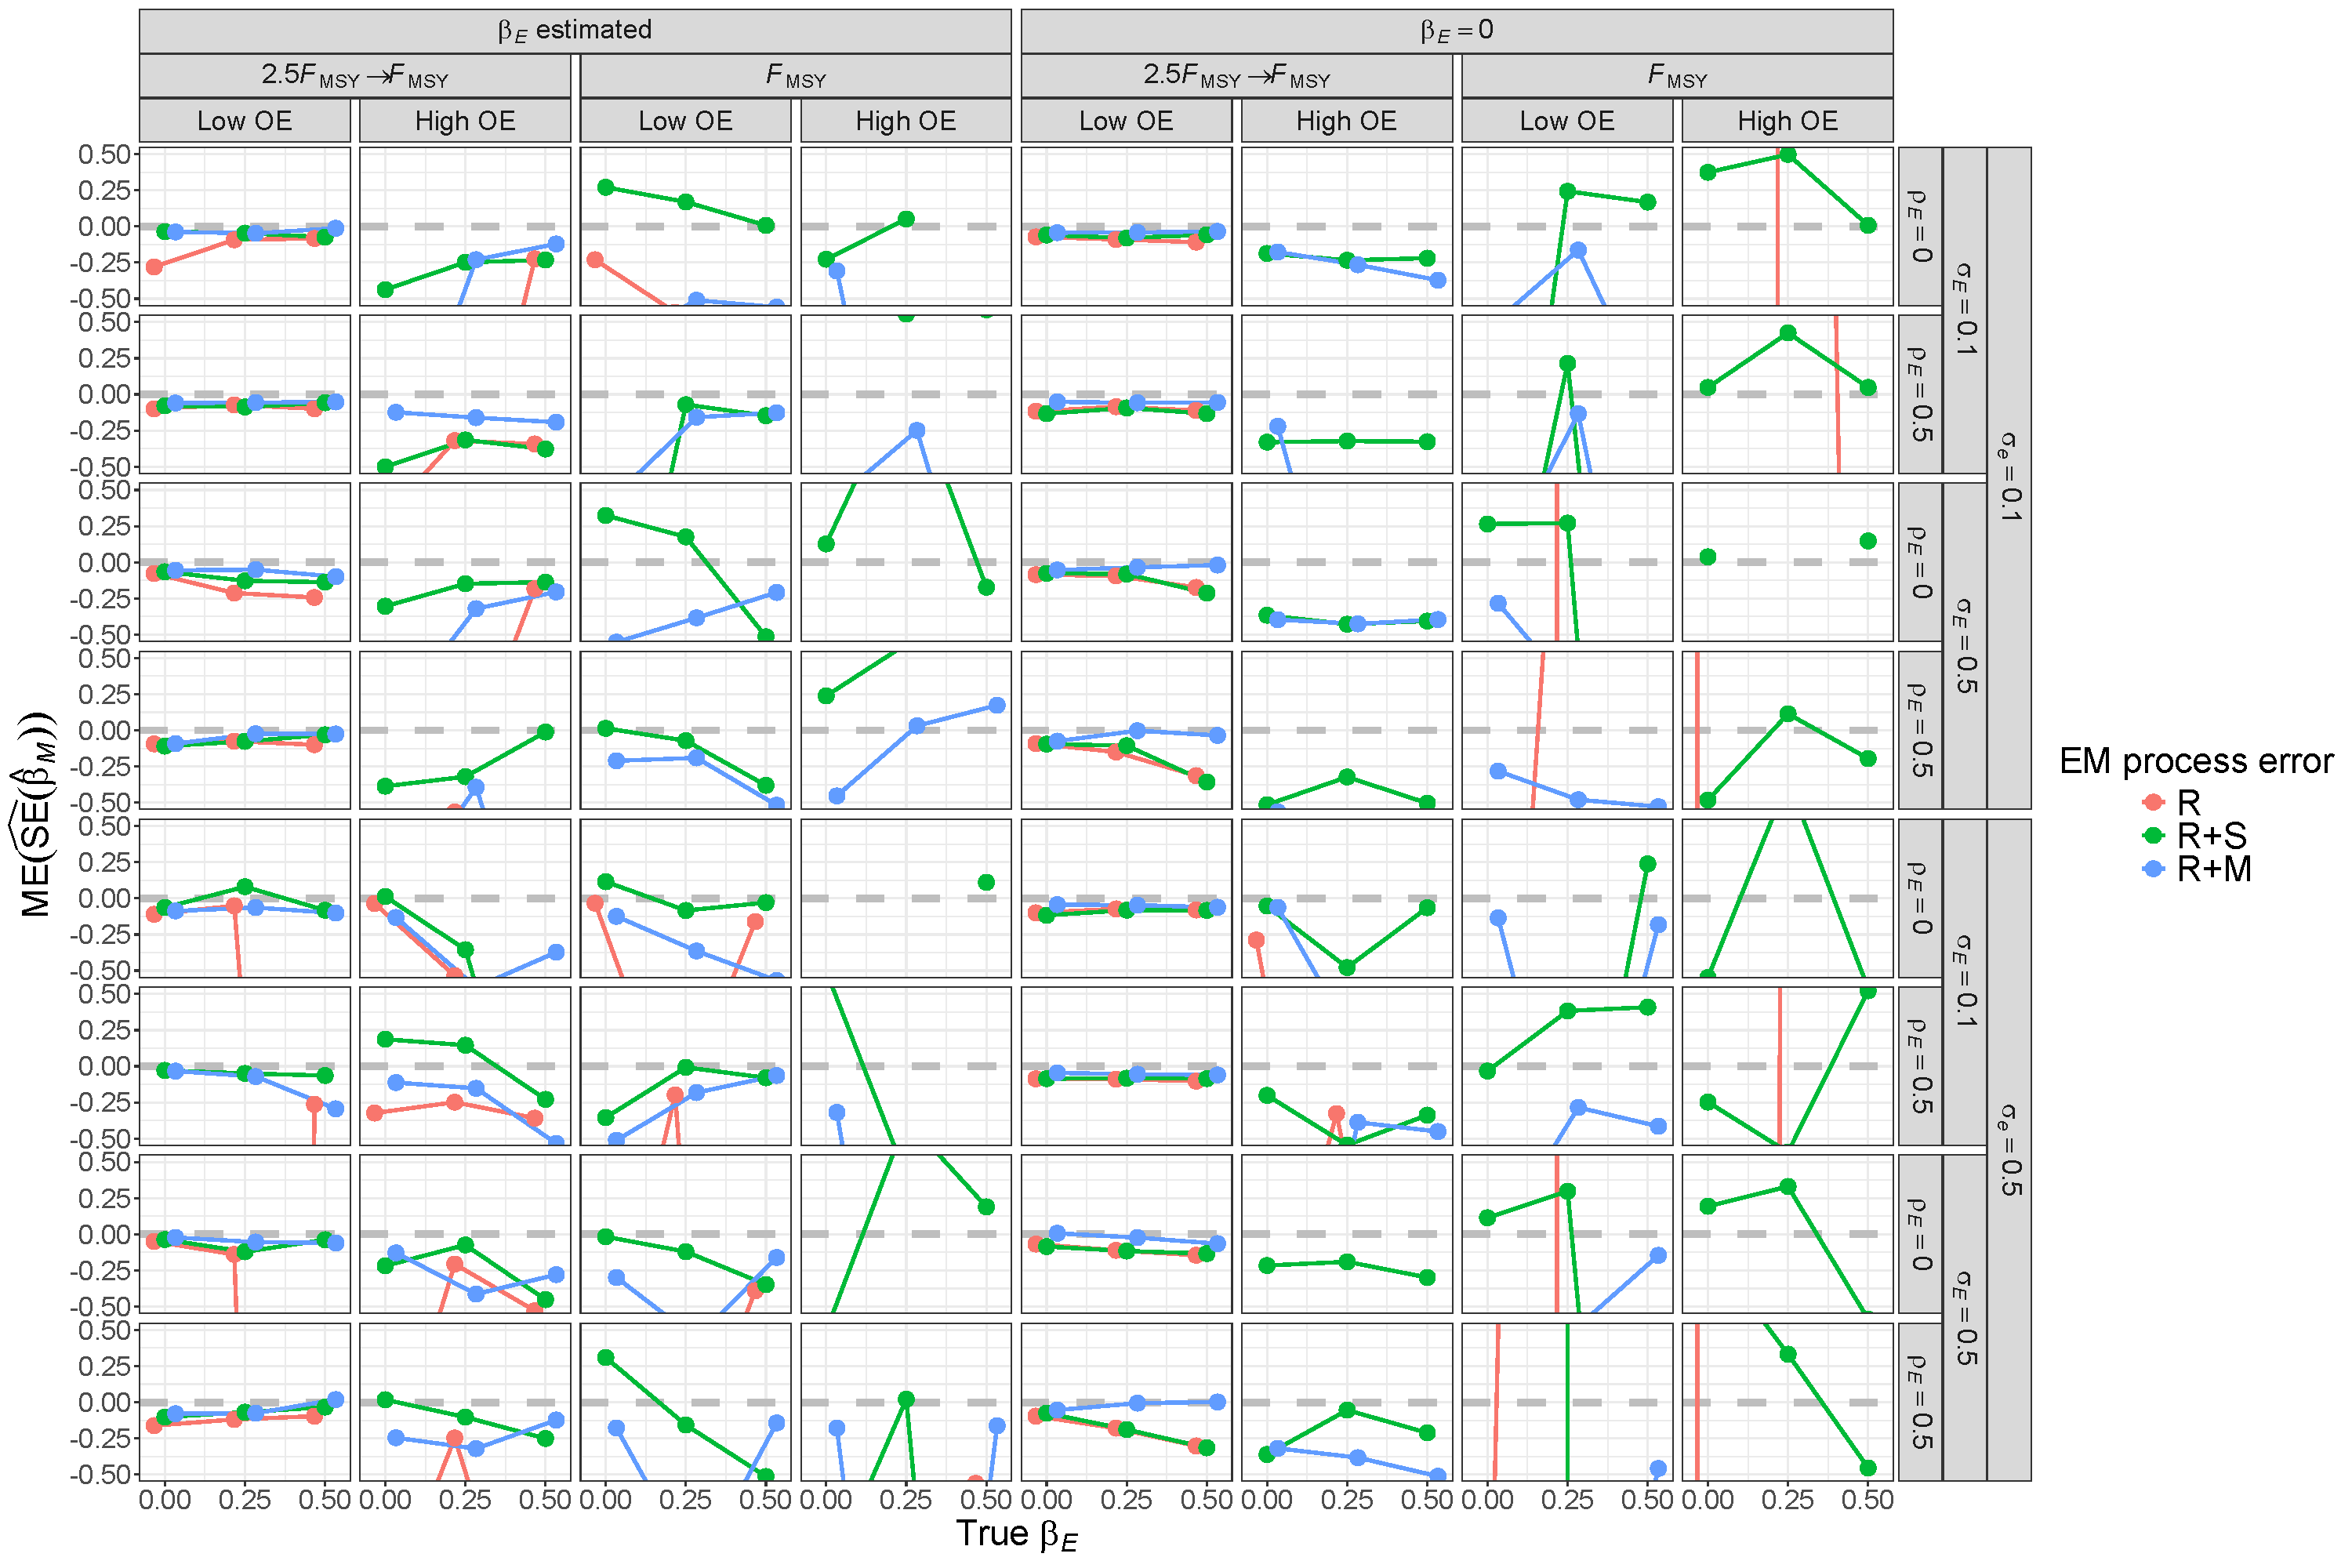
\includegraphics[height = \textheight]{se_beta_M_bias_RMom}
\end{center}
\caption{For R+M operating models, median error (ME) of Hessian-based estimates of standard error for median $M$ parameter ($\beta_M$) from fitting estimating models with alternative process error assumptions and treatment of the covariate effect ($\beta_ E= 0$ or estimated). True standard error is defined as the mean of the standard error estimates accross converged fits to simulated data sets for a given operating model scenario.}\label{se_beta_M_bias_RMom}
\end{figure}
\end{landscape}

\begin{landscape}
\begin{figure}
\begin{center}
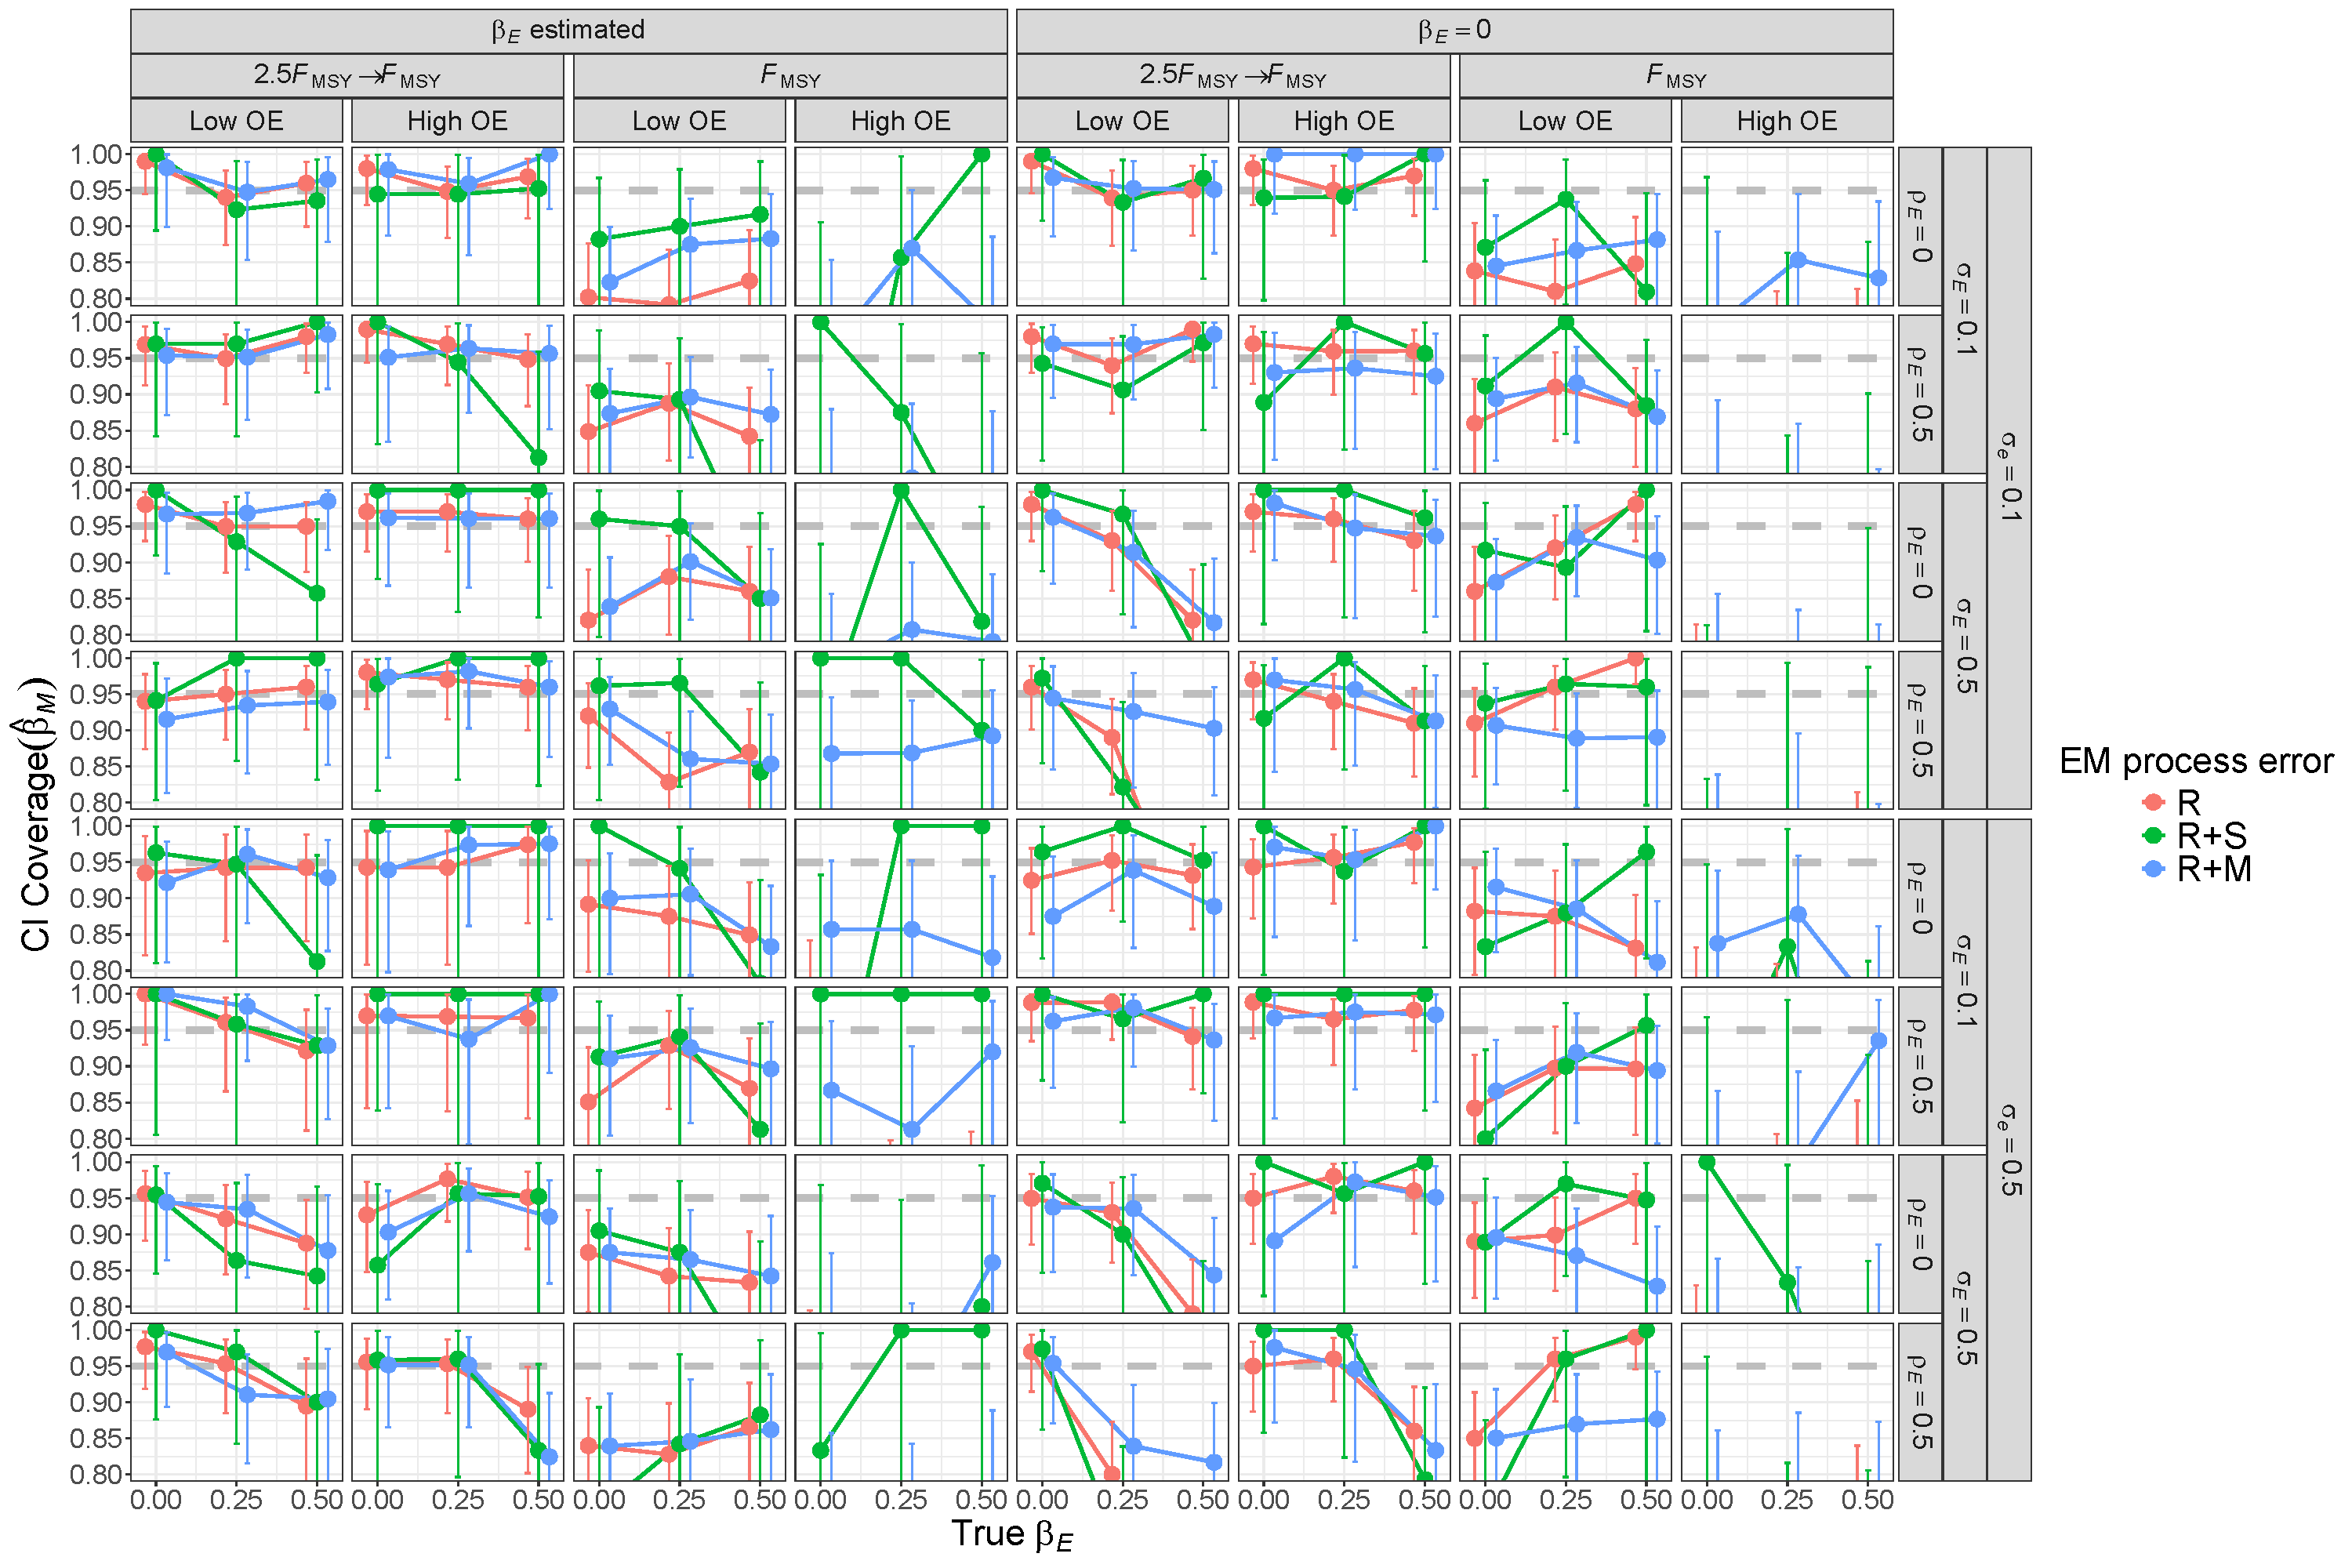
\includegraphics[height = \textheight]{beta_M_CI_coverage_Rom}
\end{center}
\caption{For R operating models, probability of 95\% confidence interval for $\beta_M$ containing the true value for estimating models with alternative process error assumptions and treatment of covariate effect ($\beta_E = 0$ or estimated). Vertical lines represent 95\% confidence intervals.}\label{beta_M_CI_coverage_Rom}
\end{figure}
\end{landscape}

\begin{landscape}
\begin{figure}
\begin{center}
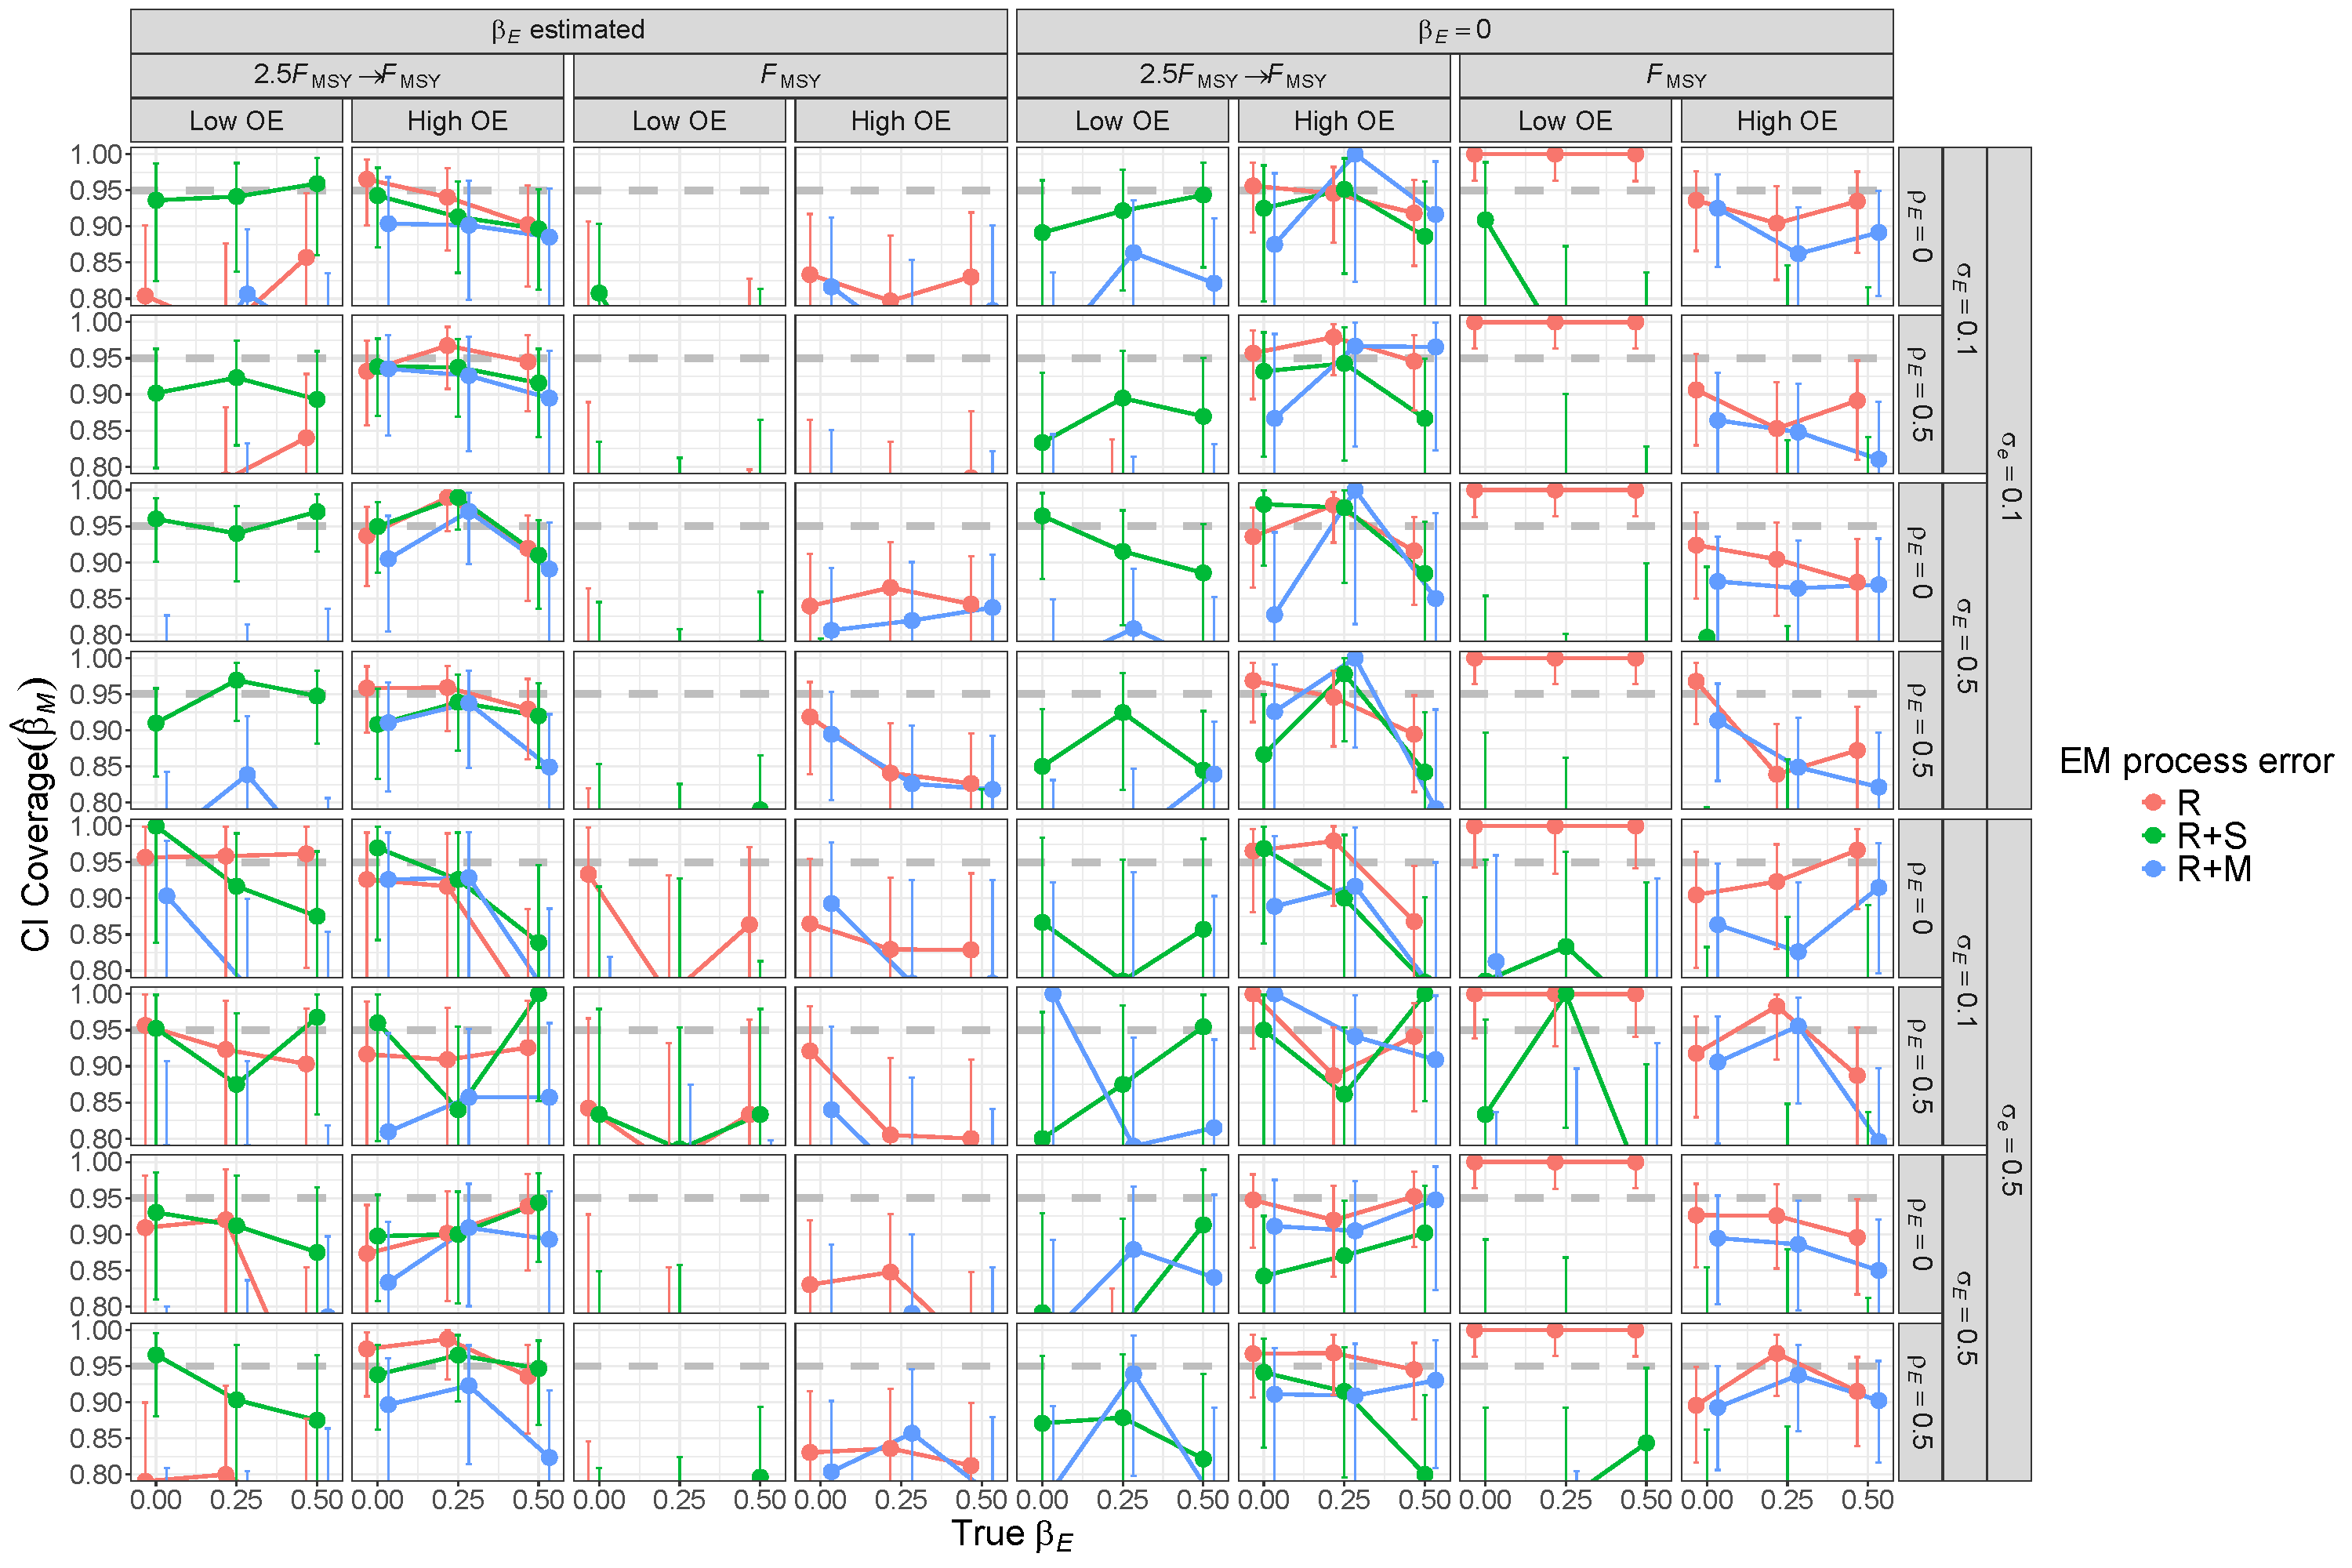
\includegraphics[height = \textheight]{beta_M_CI_coverage_RSom}
\end{center}
\caption{For R+S operating models, probability of 95\% confidence interval for $\beta_M$ containing the true value for estimating models with alternative process error assumptions and treatment of covariate effect ($\beta_E = 0$ or estimated). Vertical lines represent 95\% confidence intervals.}\label{beta_M_CI_coverage_RSom}
\end{figure}
\end{landscape}

\begin{landscape}
\begin{figure}
\begin{center}
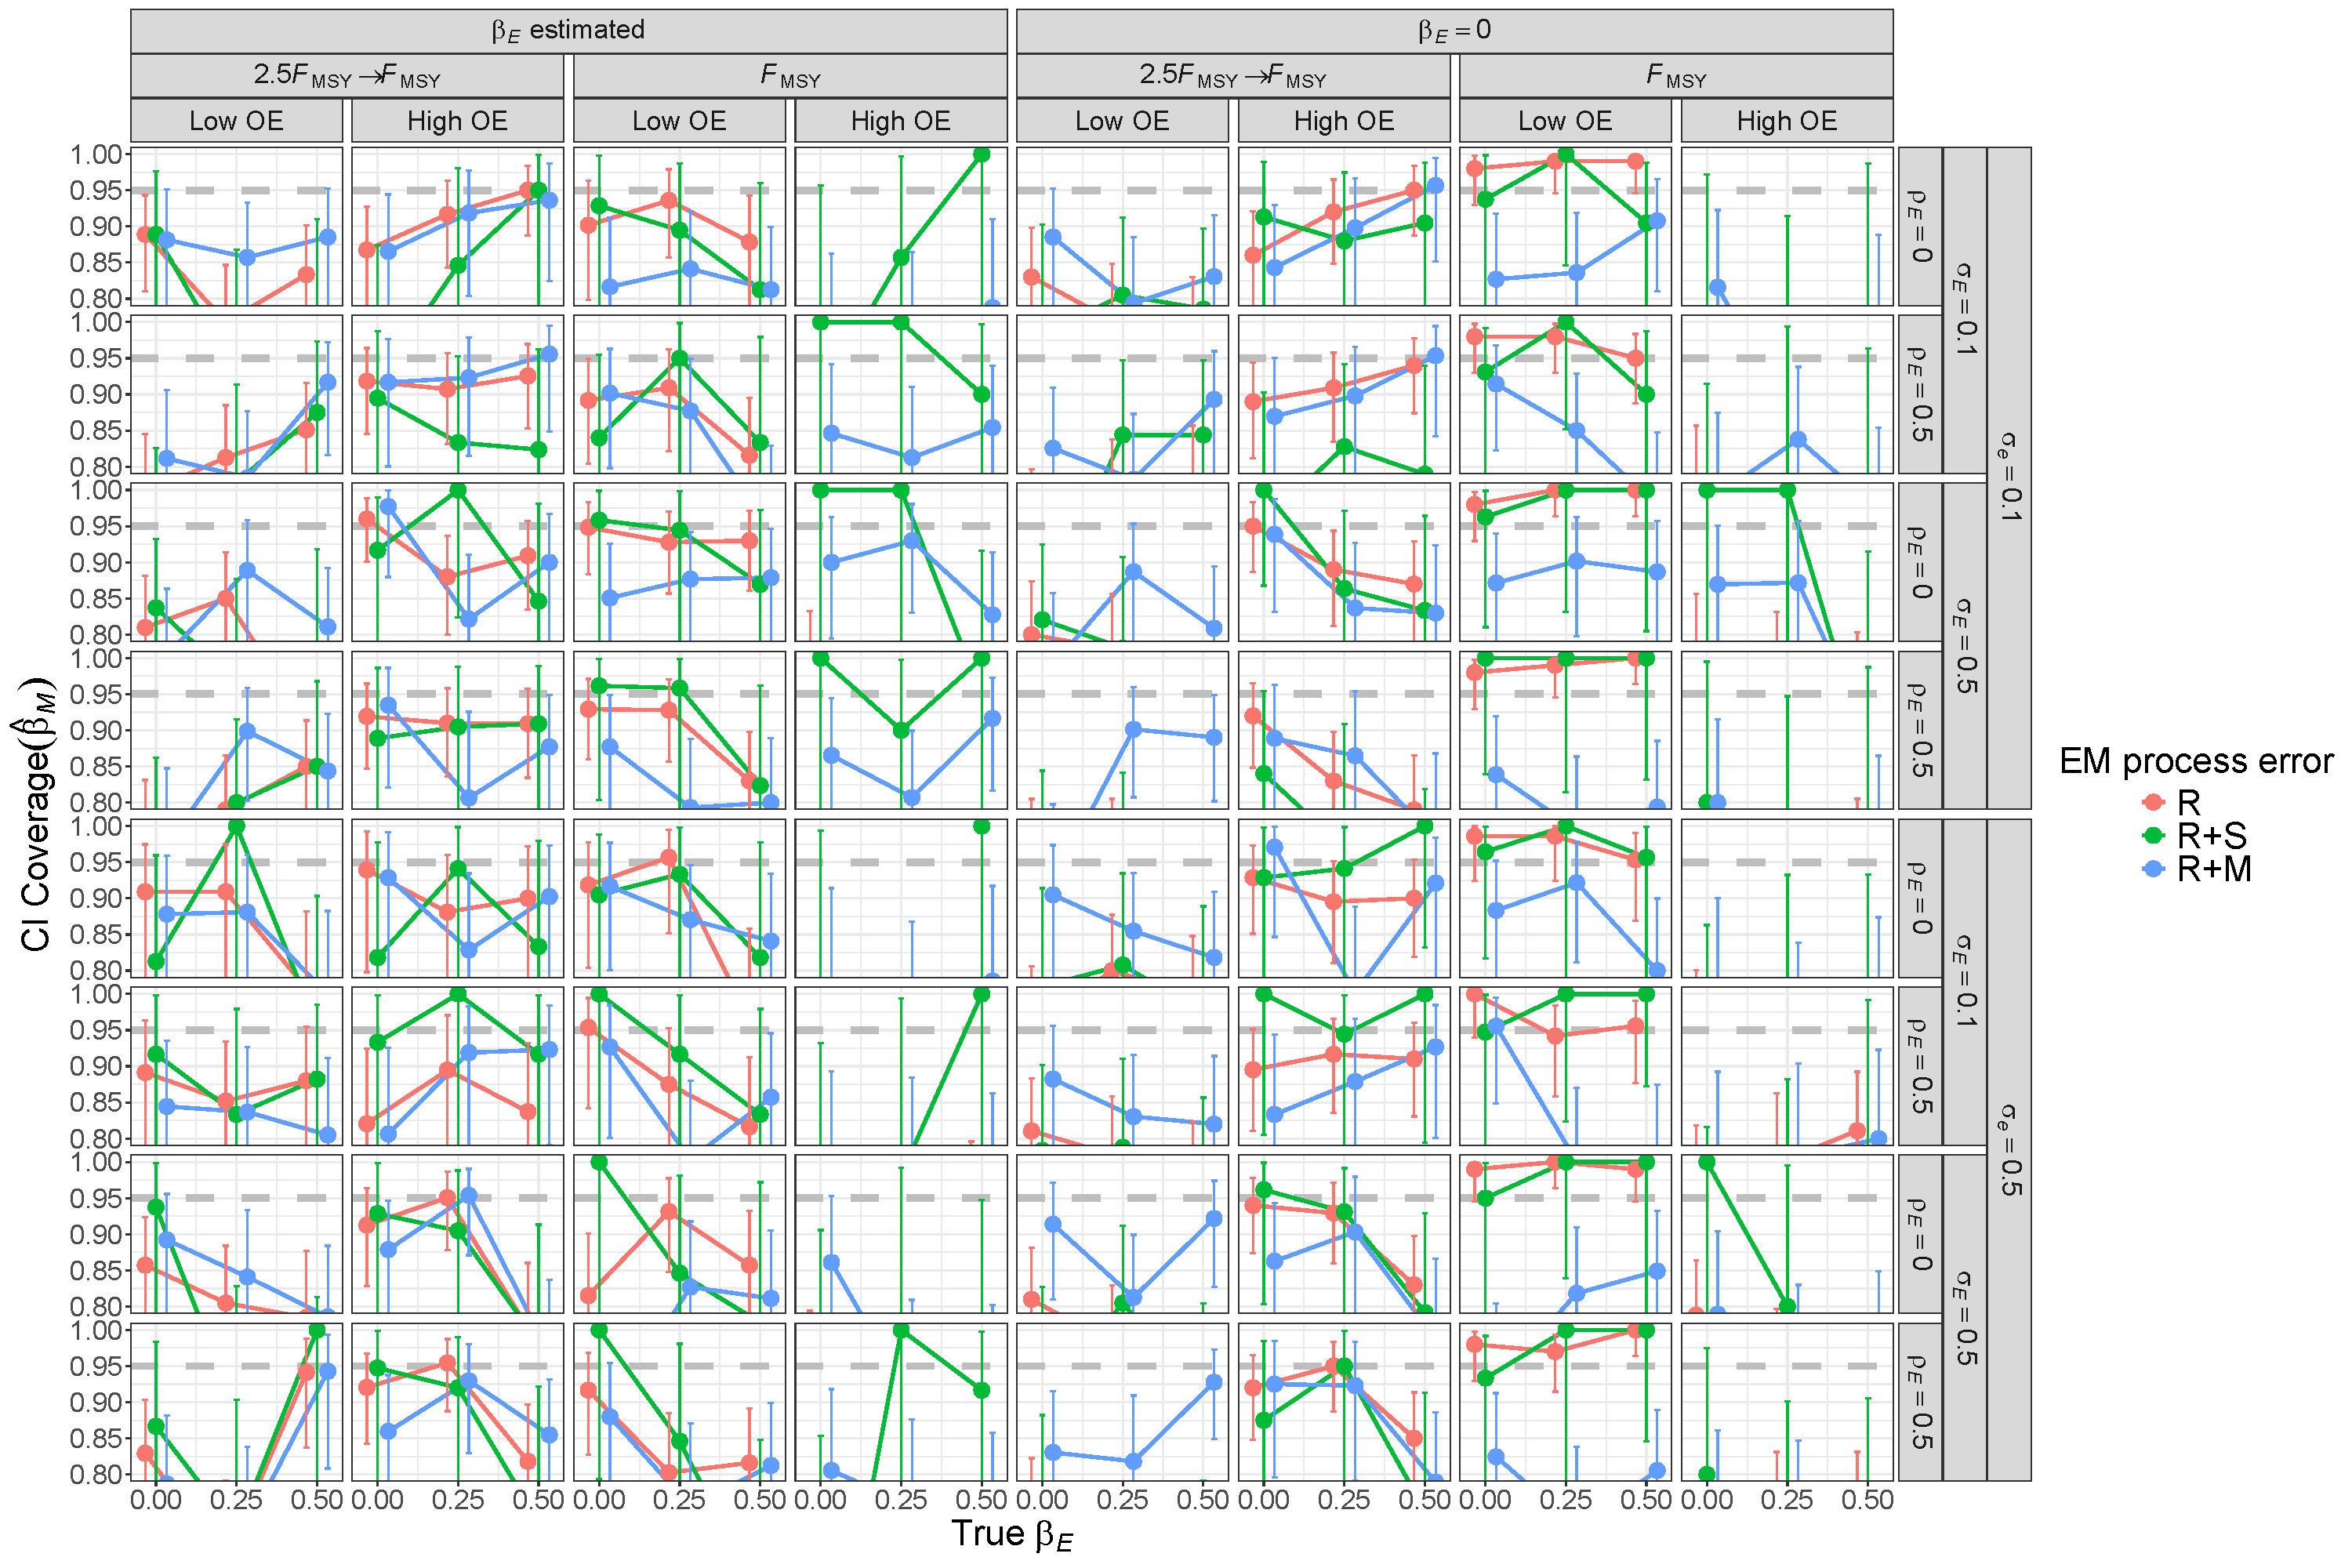
\includegraphics[height = \textheight]{beta_M_CI_coverage_RMom}
\end{center}
\caption{For R+M operating models, probability of 95\% confidence interval for $\beta_M$ containing the true value for estimating models with alternative process error assumptions and treatment of covariate effect ($\beta_E = 0$ or estimated). Vertical lines represent 95\% confidence intervals.}\label{beta_M_CI_coverage_RMom}
\end{figure}
\end{landscape}

\begin{landscape}
\begin{figure}
\begin{center}
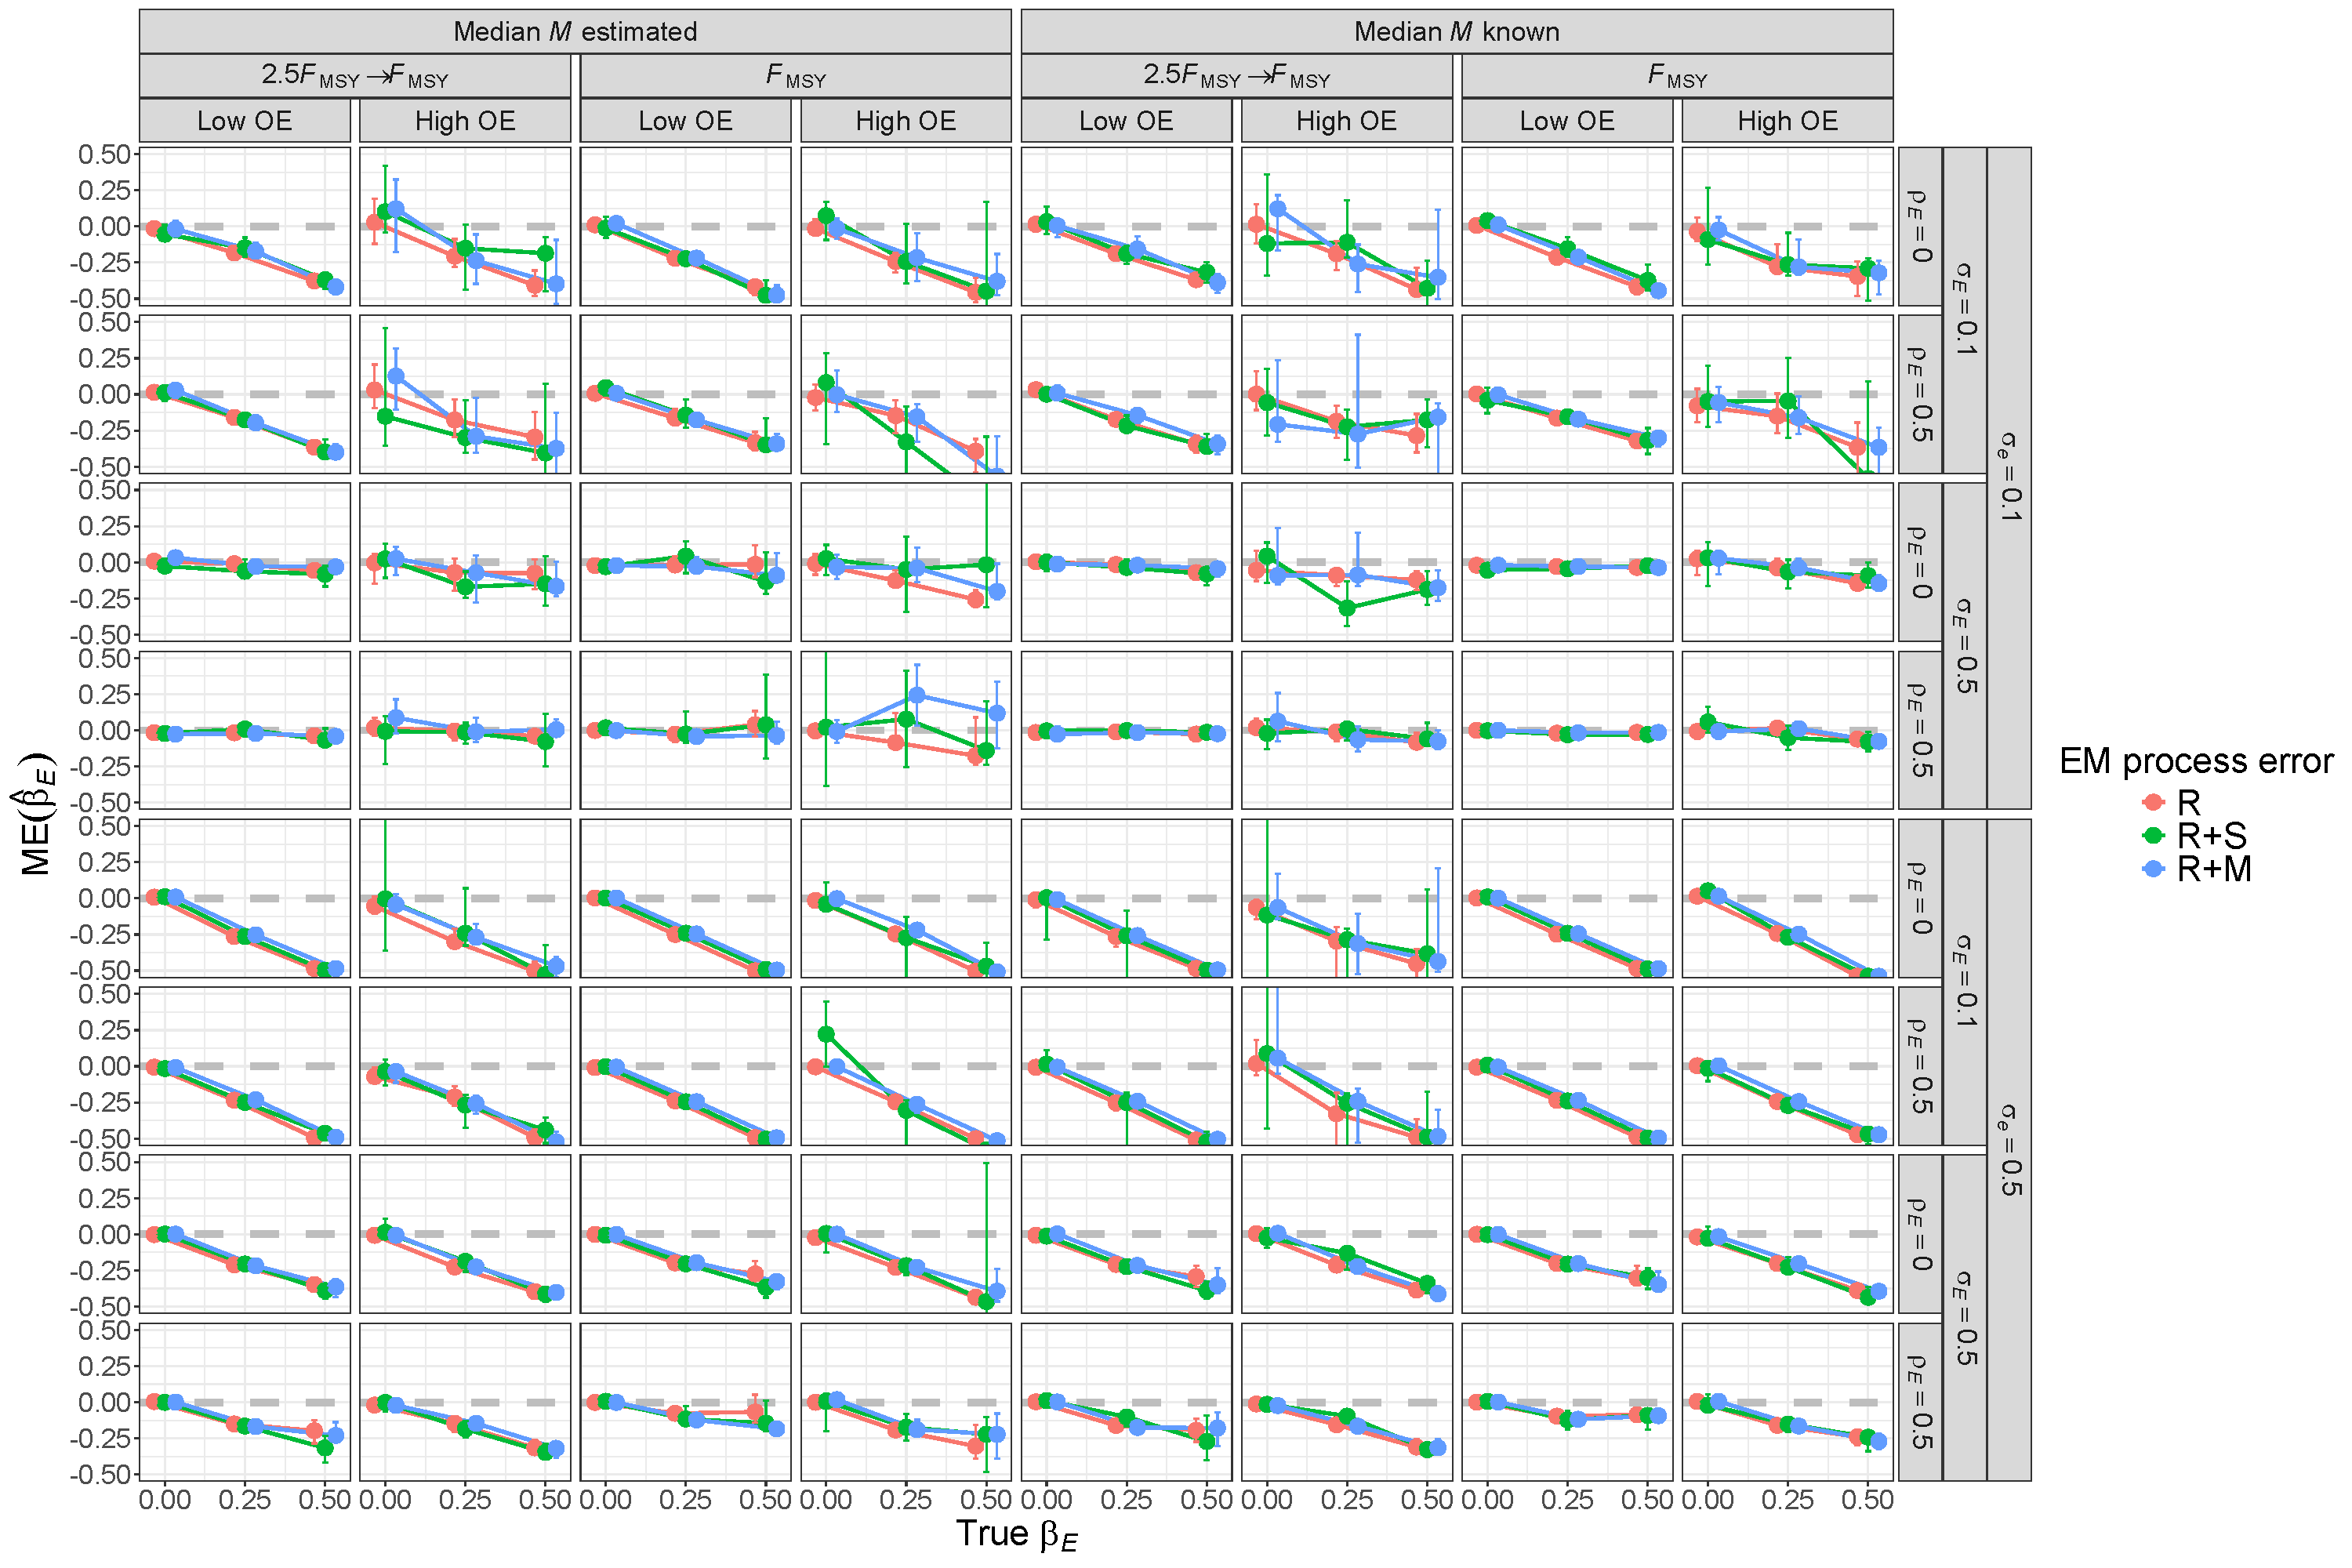
\includegraphics[height = \textheight]{beta_E_bias_Rom}
\end{center}
\caption{For R operating models, median error (ME) of estimates of environmental effect on $M$ ($\beta_E$) from fitting estimating models with alternative process error assumptions and treatment of median $M$ parameter ($\beta_M$). Vertical lines represent 95\% confidence intervals.}\label{beta_E_bias_Rom}
\end{figure}
\end{landscape}

\begin{landscape}
\begin{figure}
\begin{center}
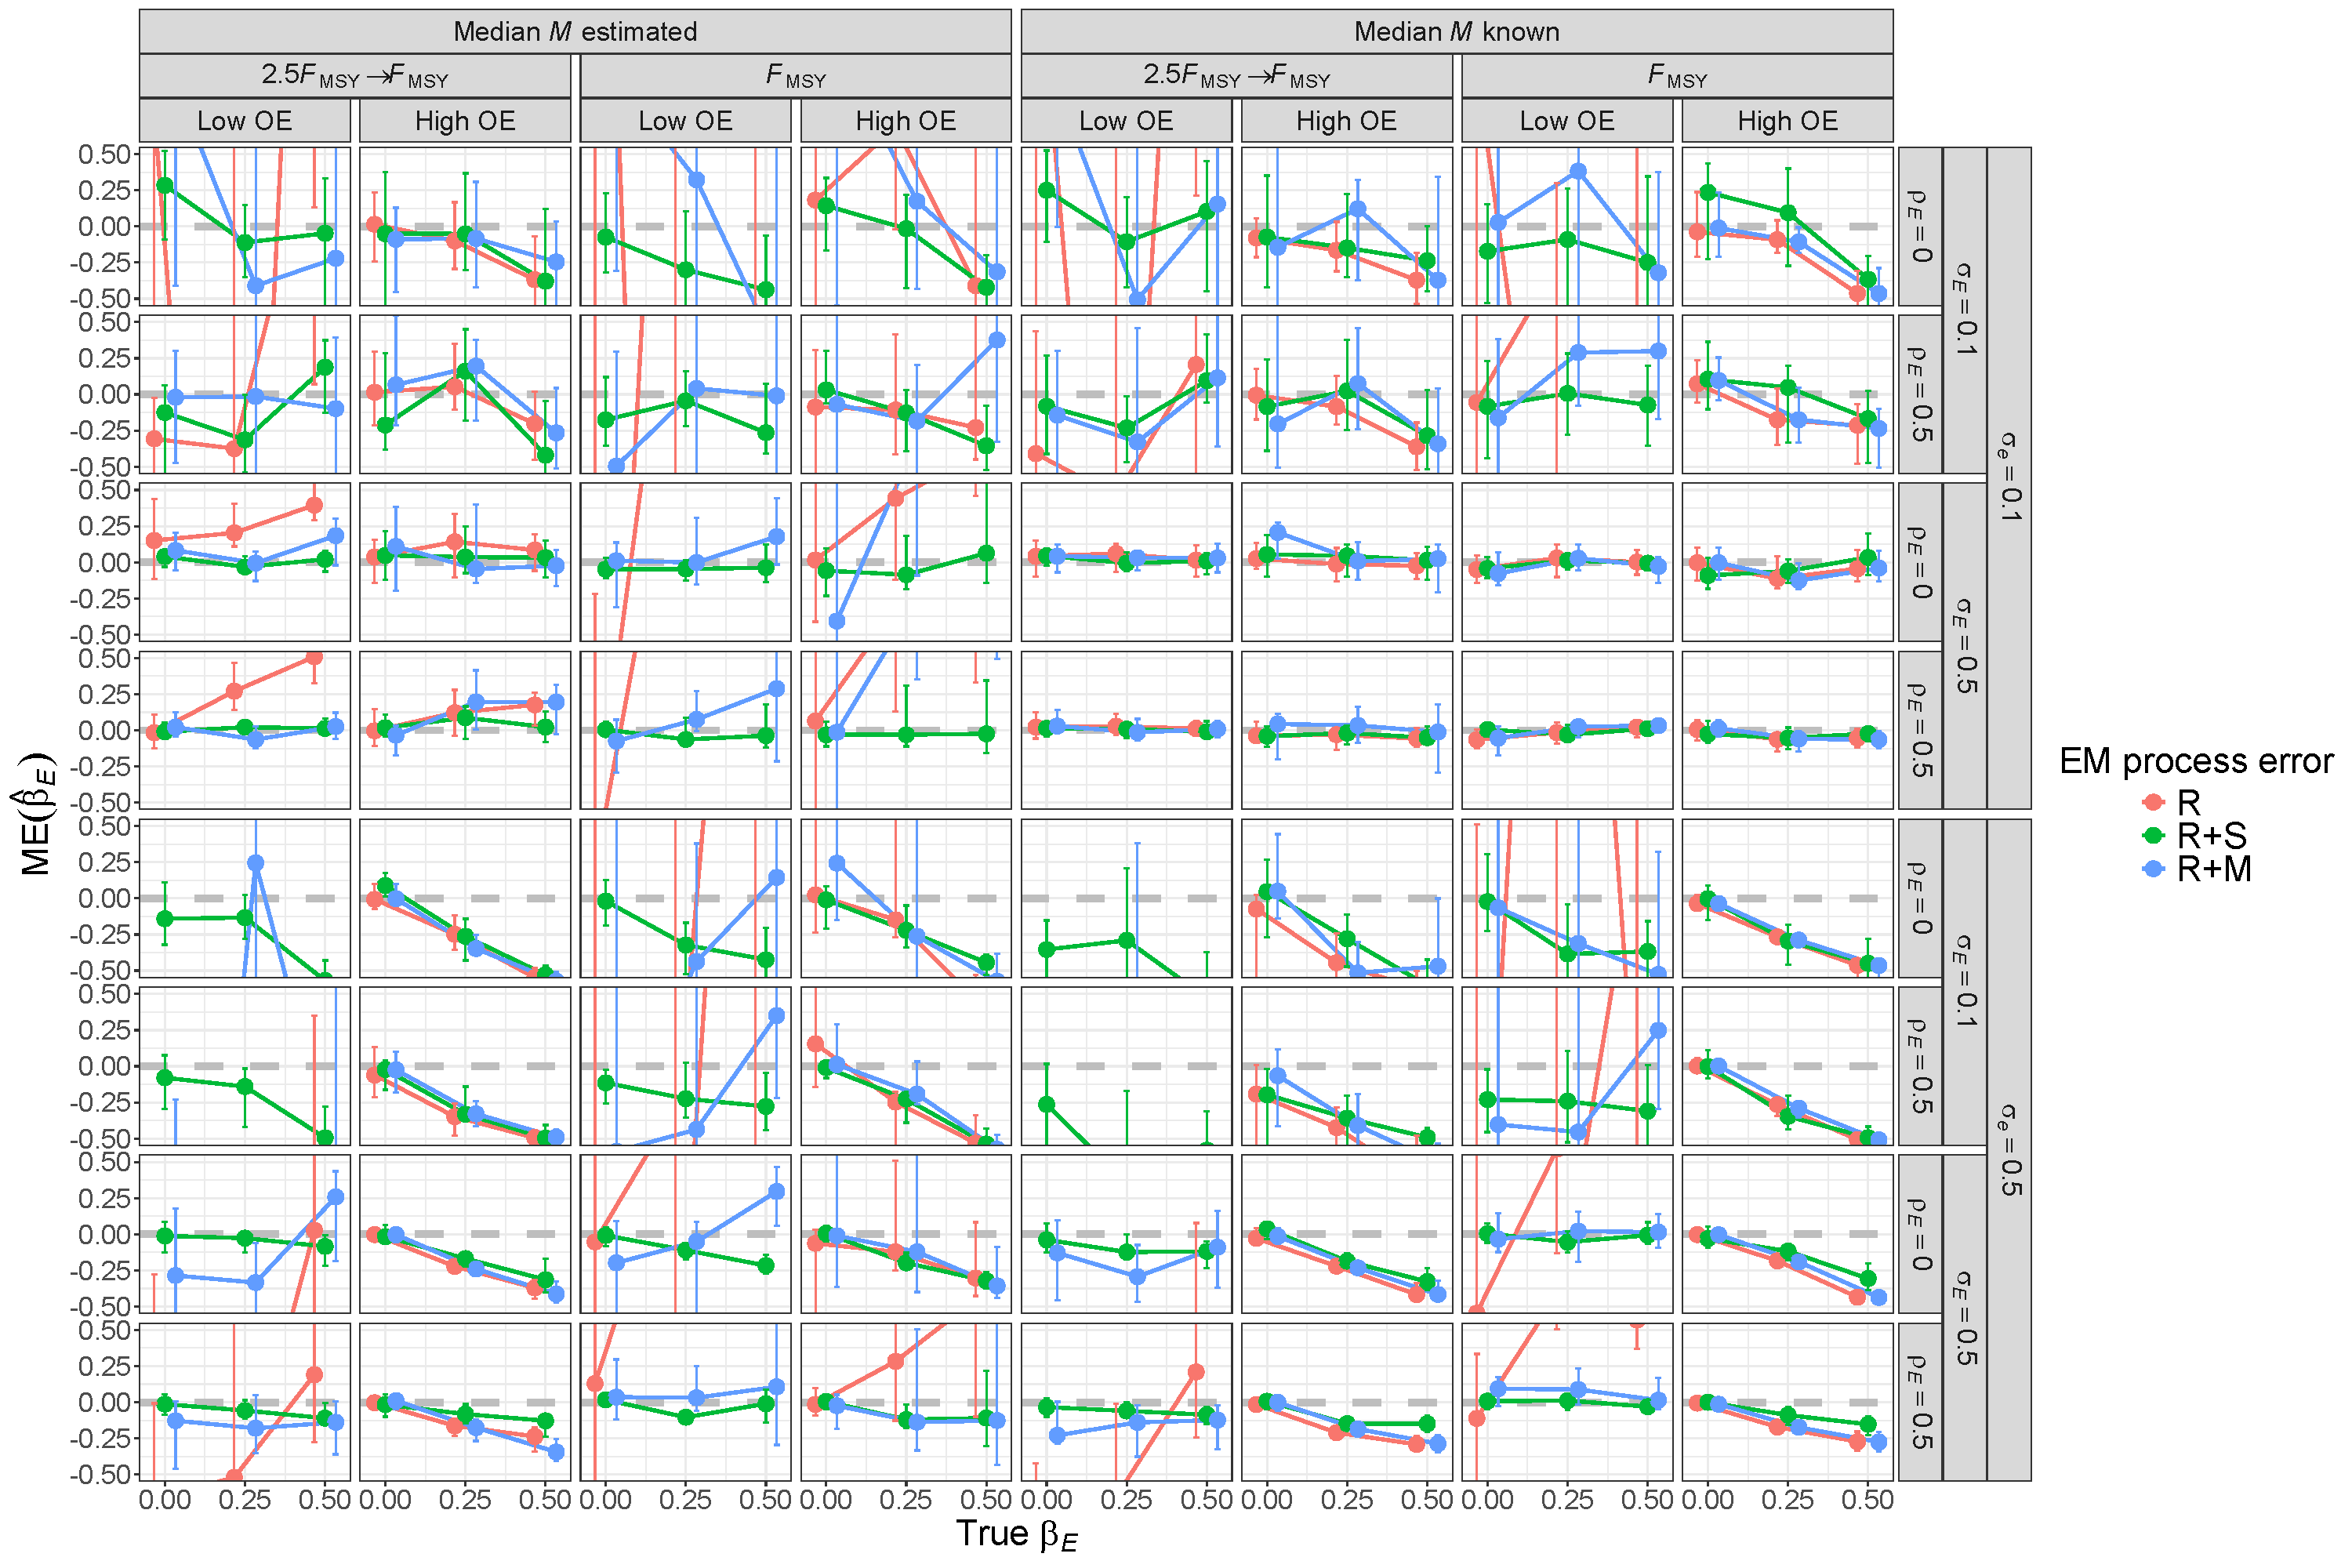
\includegraphics[height = \textheight]{beta_E_bias_RSom}
\end{center}
\caption{For R+S operating models, median error (ME) of estimates of environmental effect on $M$ ($\beta_E$) from fitting estimating models with alternative process error assumptions and treatment of median $M$ parameter ($\beta_M$). Vertical lines represent 95\% confidence intervals.}\label{beta_E_bias_RSom}
\end{figure}
\end{landscape}

\begin{landscape}
\begin{figure}
\begin{center}
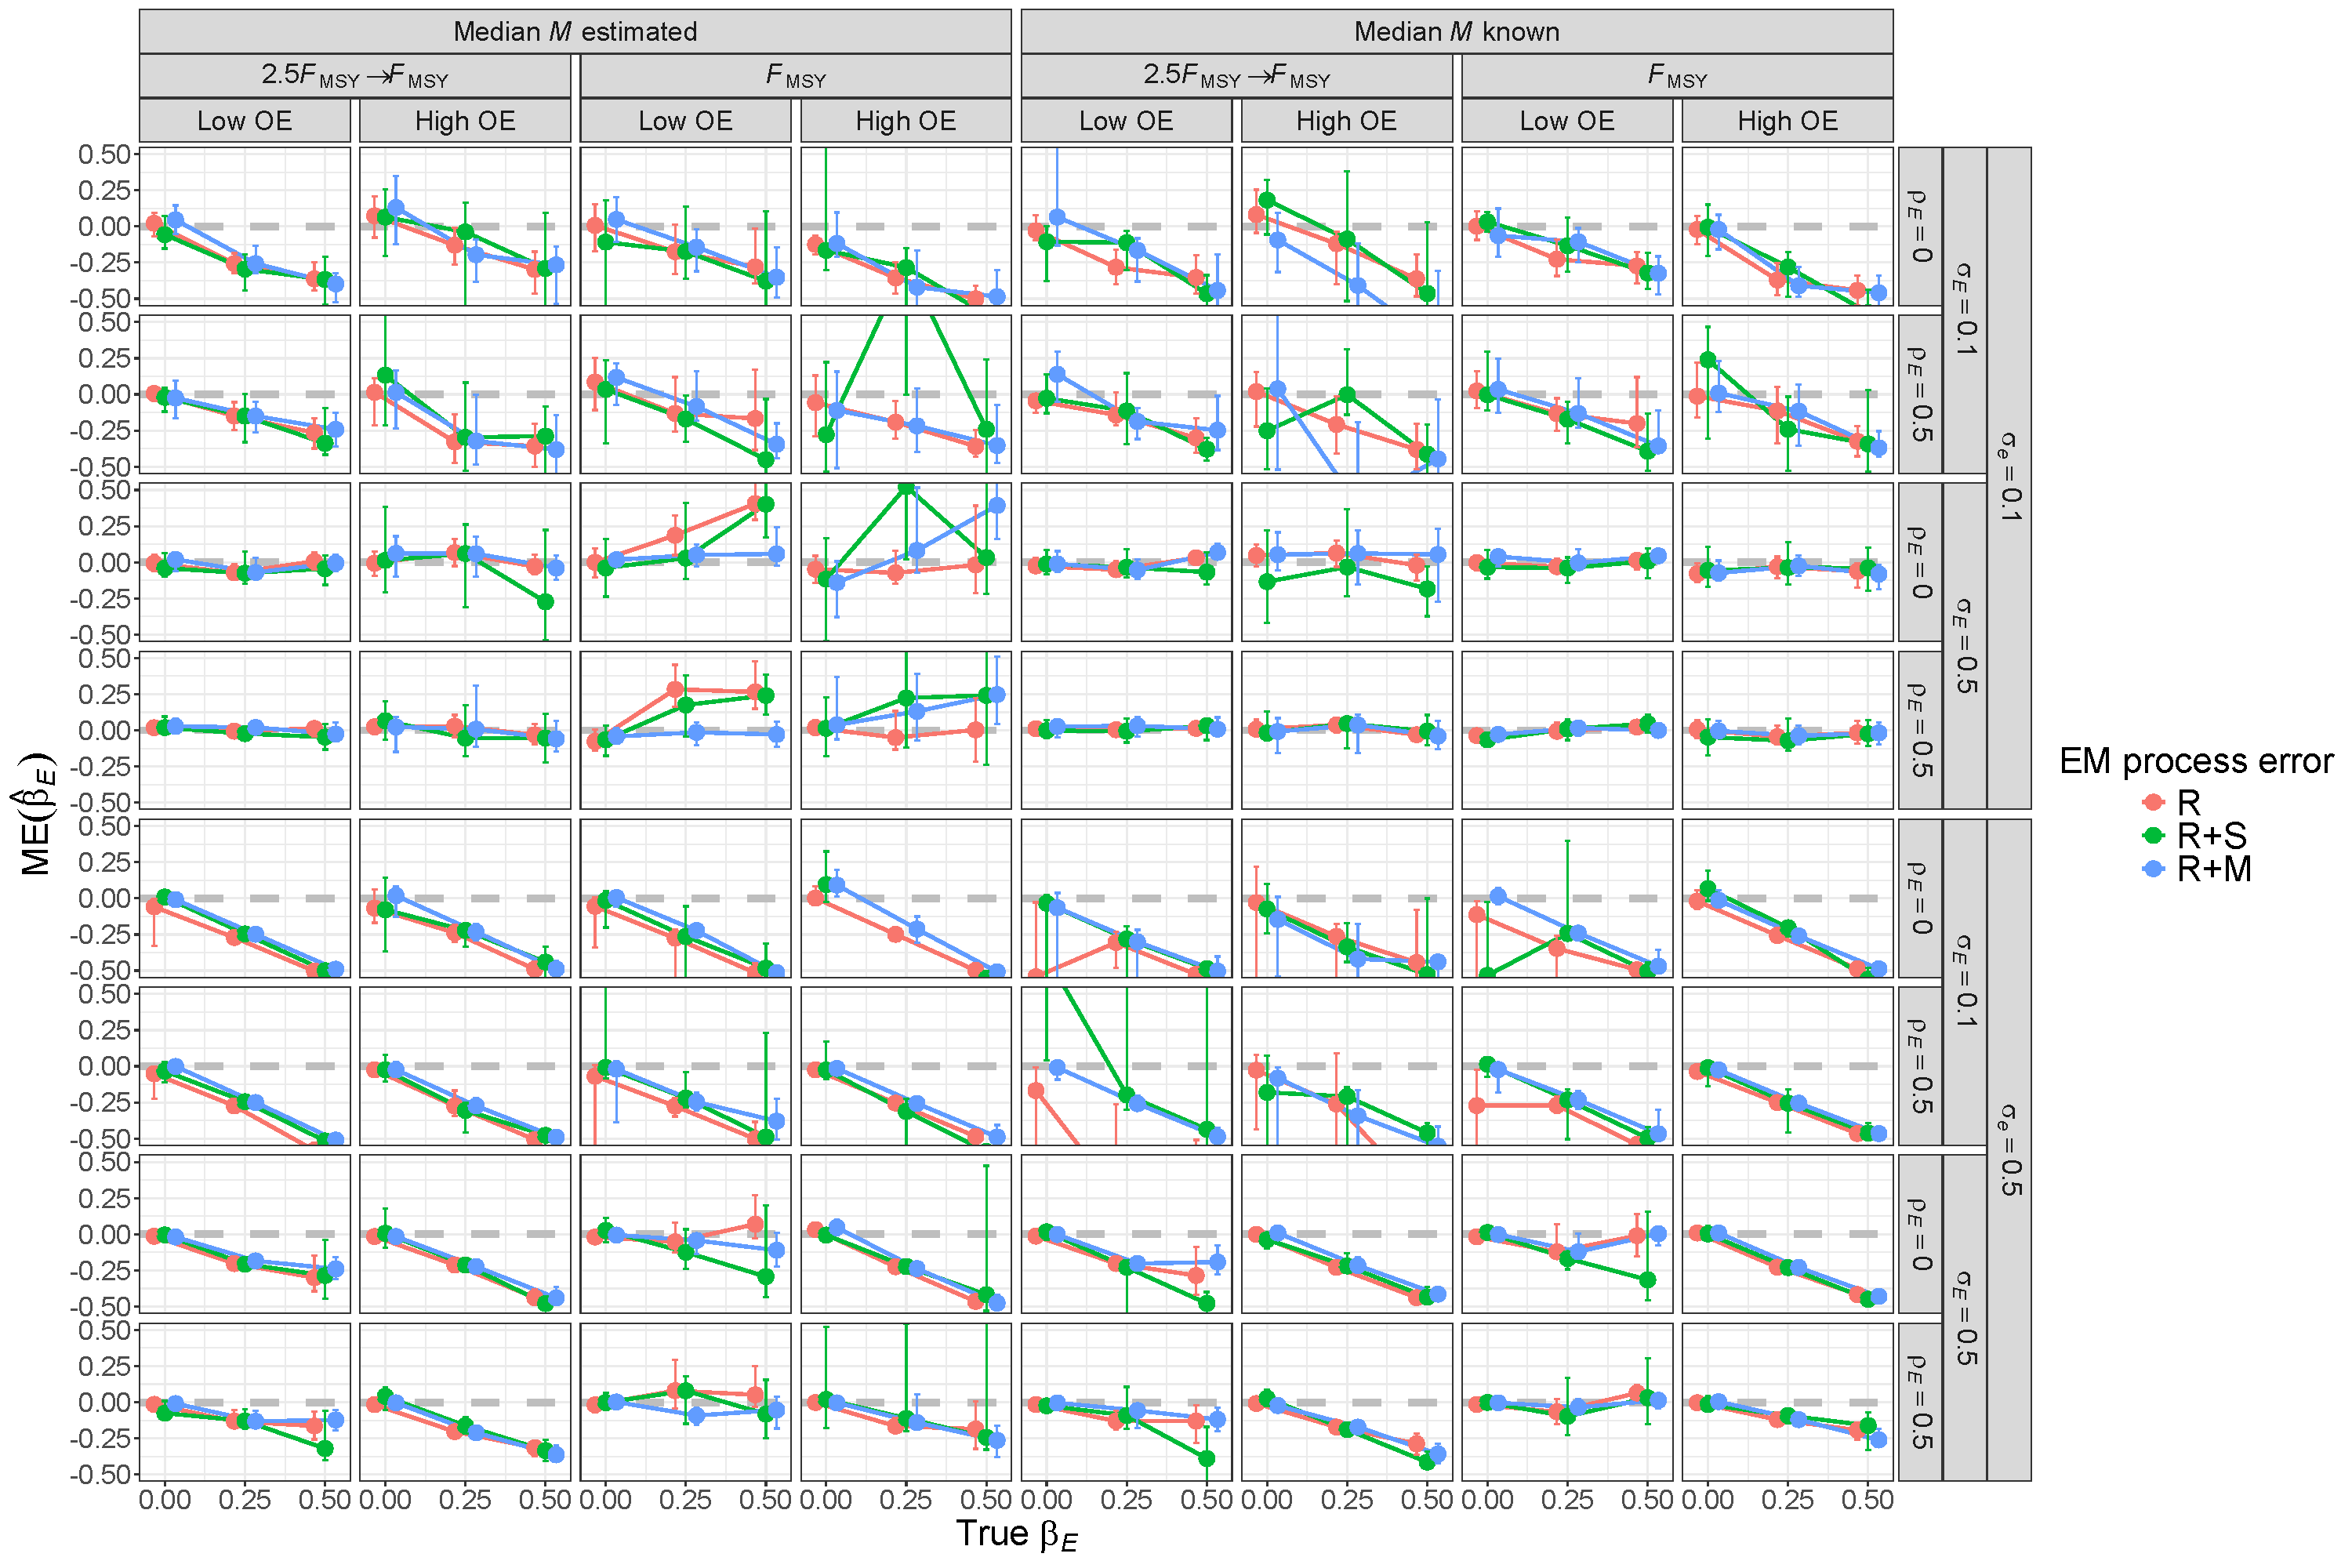
\includegraphics[height = \textheight]{beta_E_bias_RMom}
\end{center}
\caption{For R+M operating models, median error (ME) of estimates of environmental effect on $M$ ($\beta_E$) from fitting estimating models with alternative process error assumptions and treatment of median $M$ parameter ($\beta_M$). Vertical lines represent 95\% confidence intervals.}\label{beta_E_bias_RMom}
\end{figure}
\end{landscape}

\begin{landscape}
\begin{figure}
\begin{center}
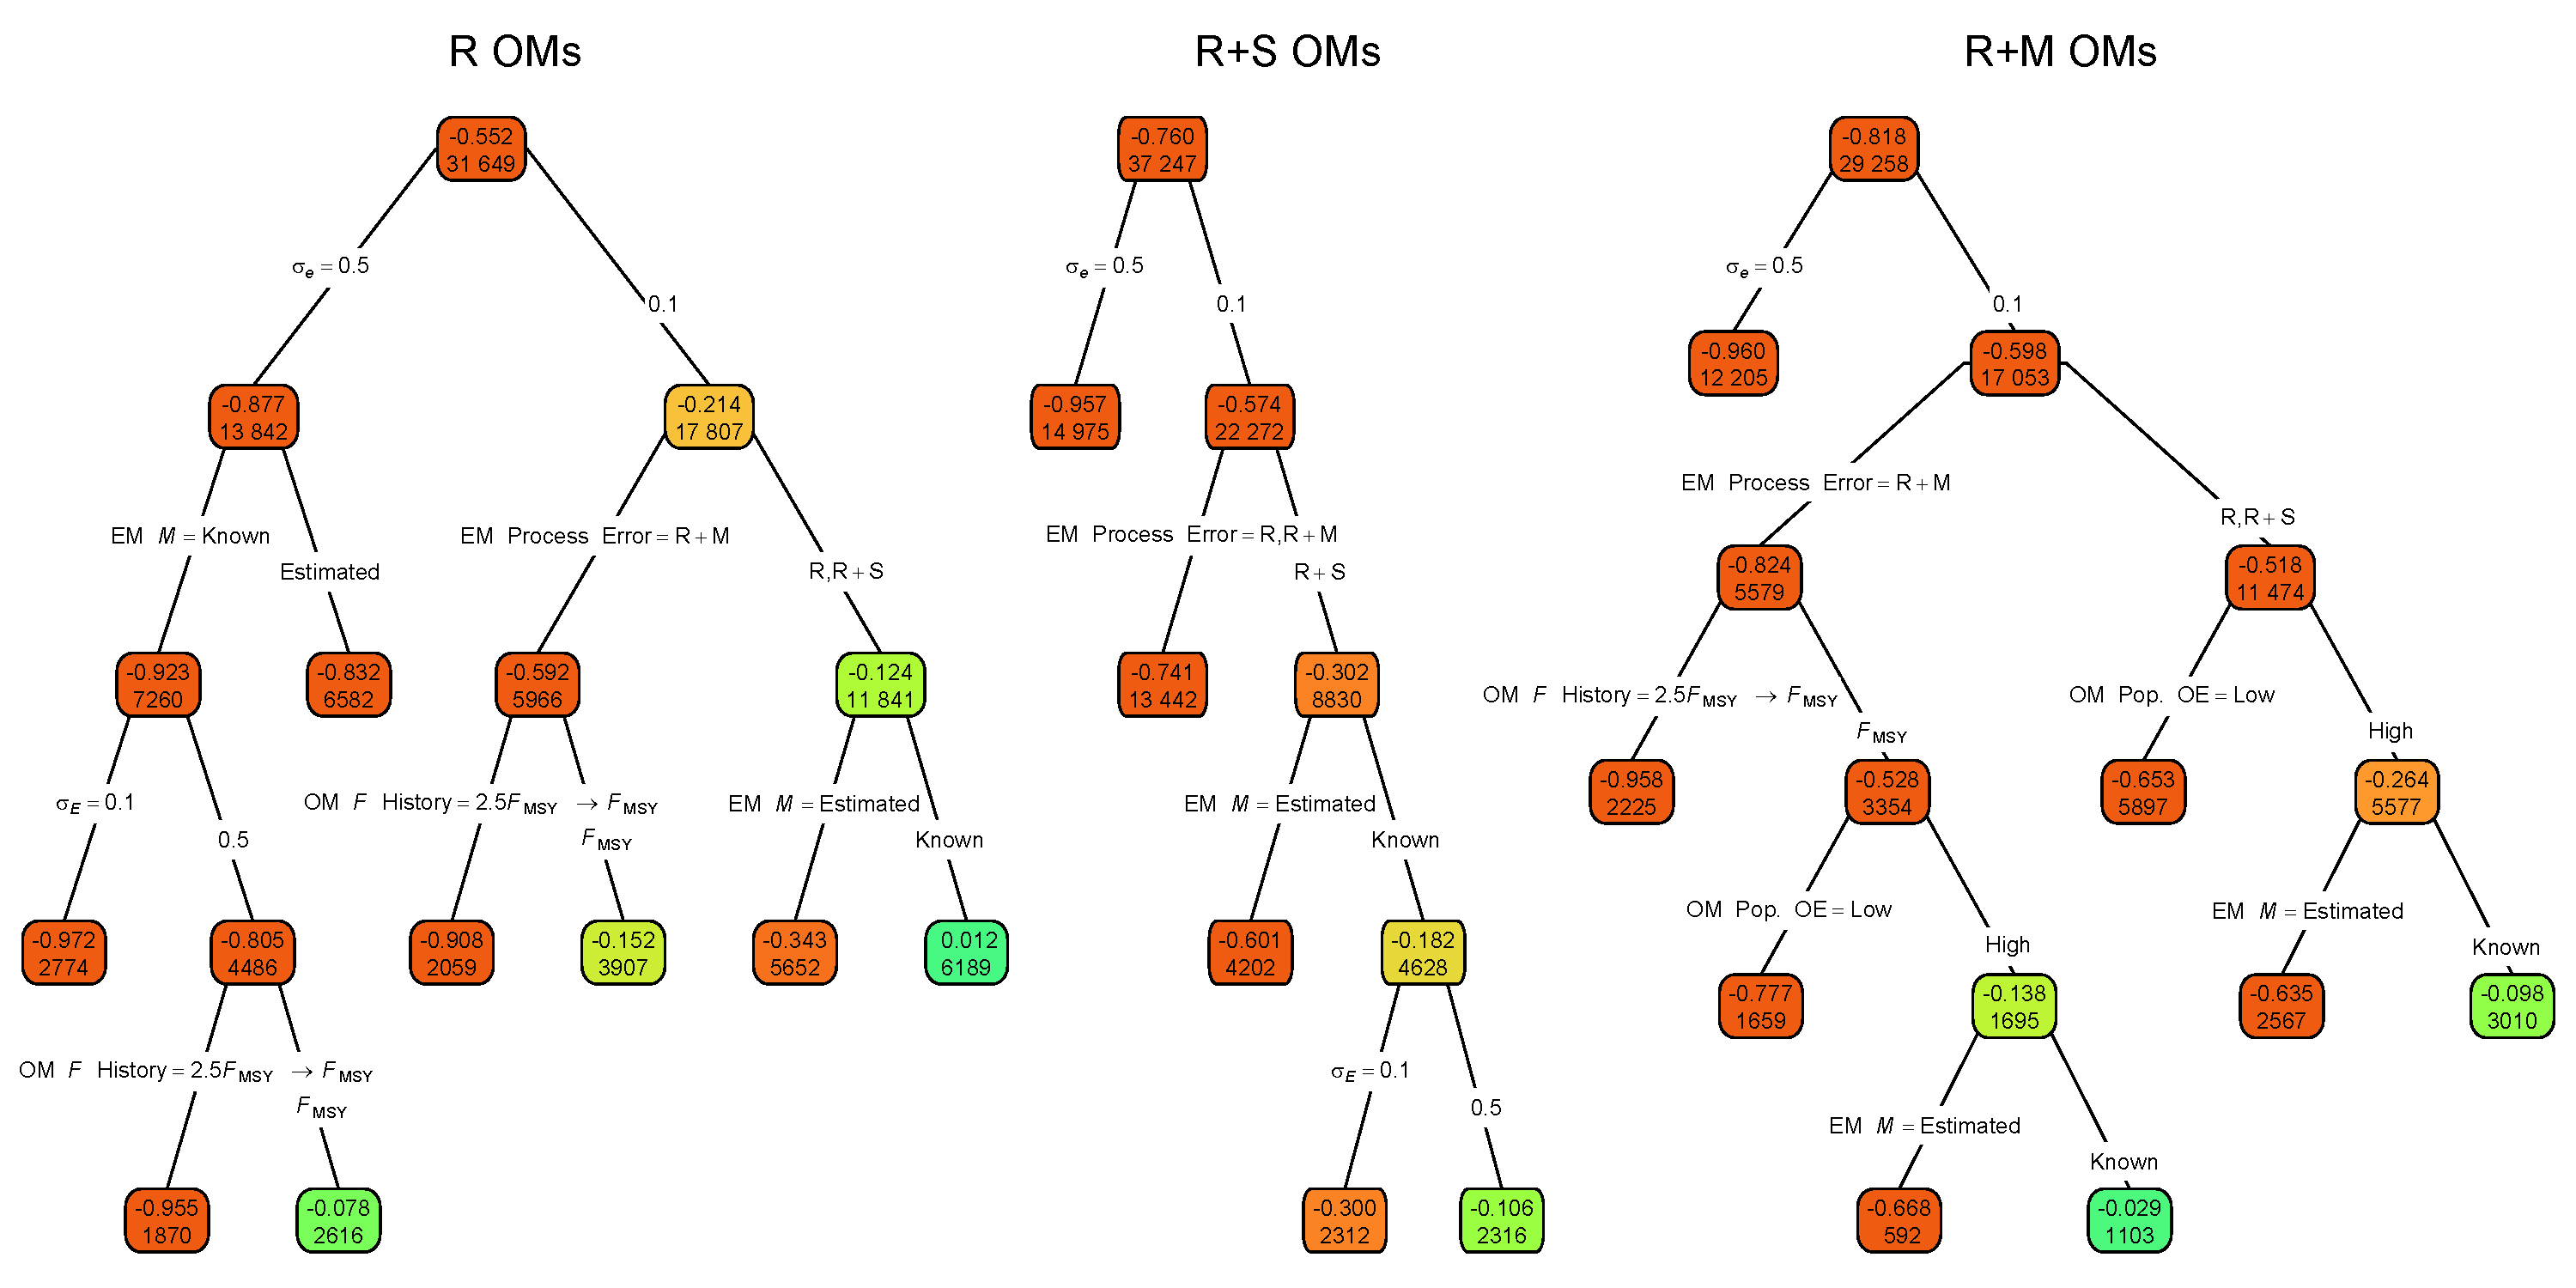
\includegraphics[width = 1.4\textwidth]{ecov_beta_SE_bias_regtree_plots}
\end{center}
\caption{Regression trees for error of the Hessian-based standard error estimates for covariate effect on $M$ ($\widehat {\text{SE}}\left(\widehat \beta_E\right)$). Each node shows the median error for the corresponding subset. Lower or higher absolute median errors are indicated by more green or red polygons, respectively. See Figure \ref{conv_class} caption and Table \ref{factor_table} for further details.}\label{ecov_effect_SE_bias_regtree}
\end{figure}
\end{landscape}

\begin{landscape}
\begin{figure}
\begin{center}
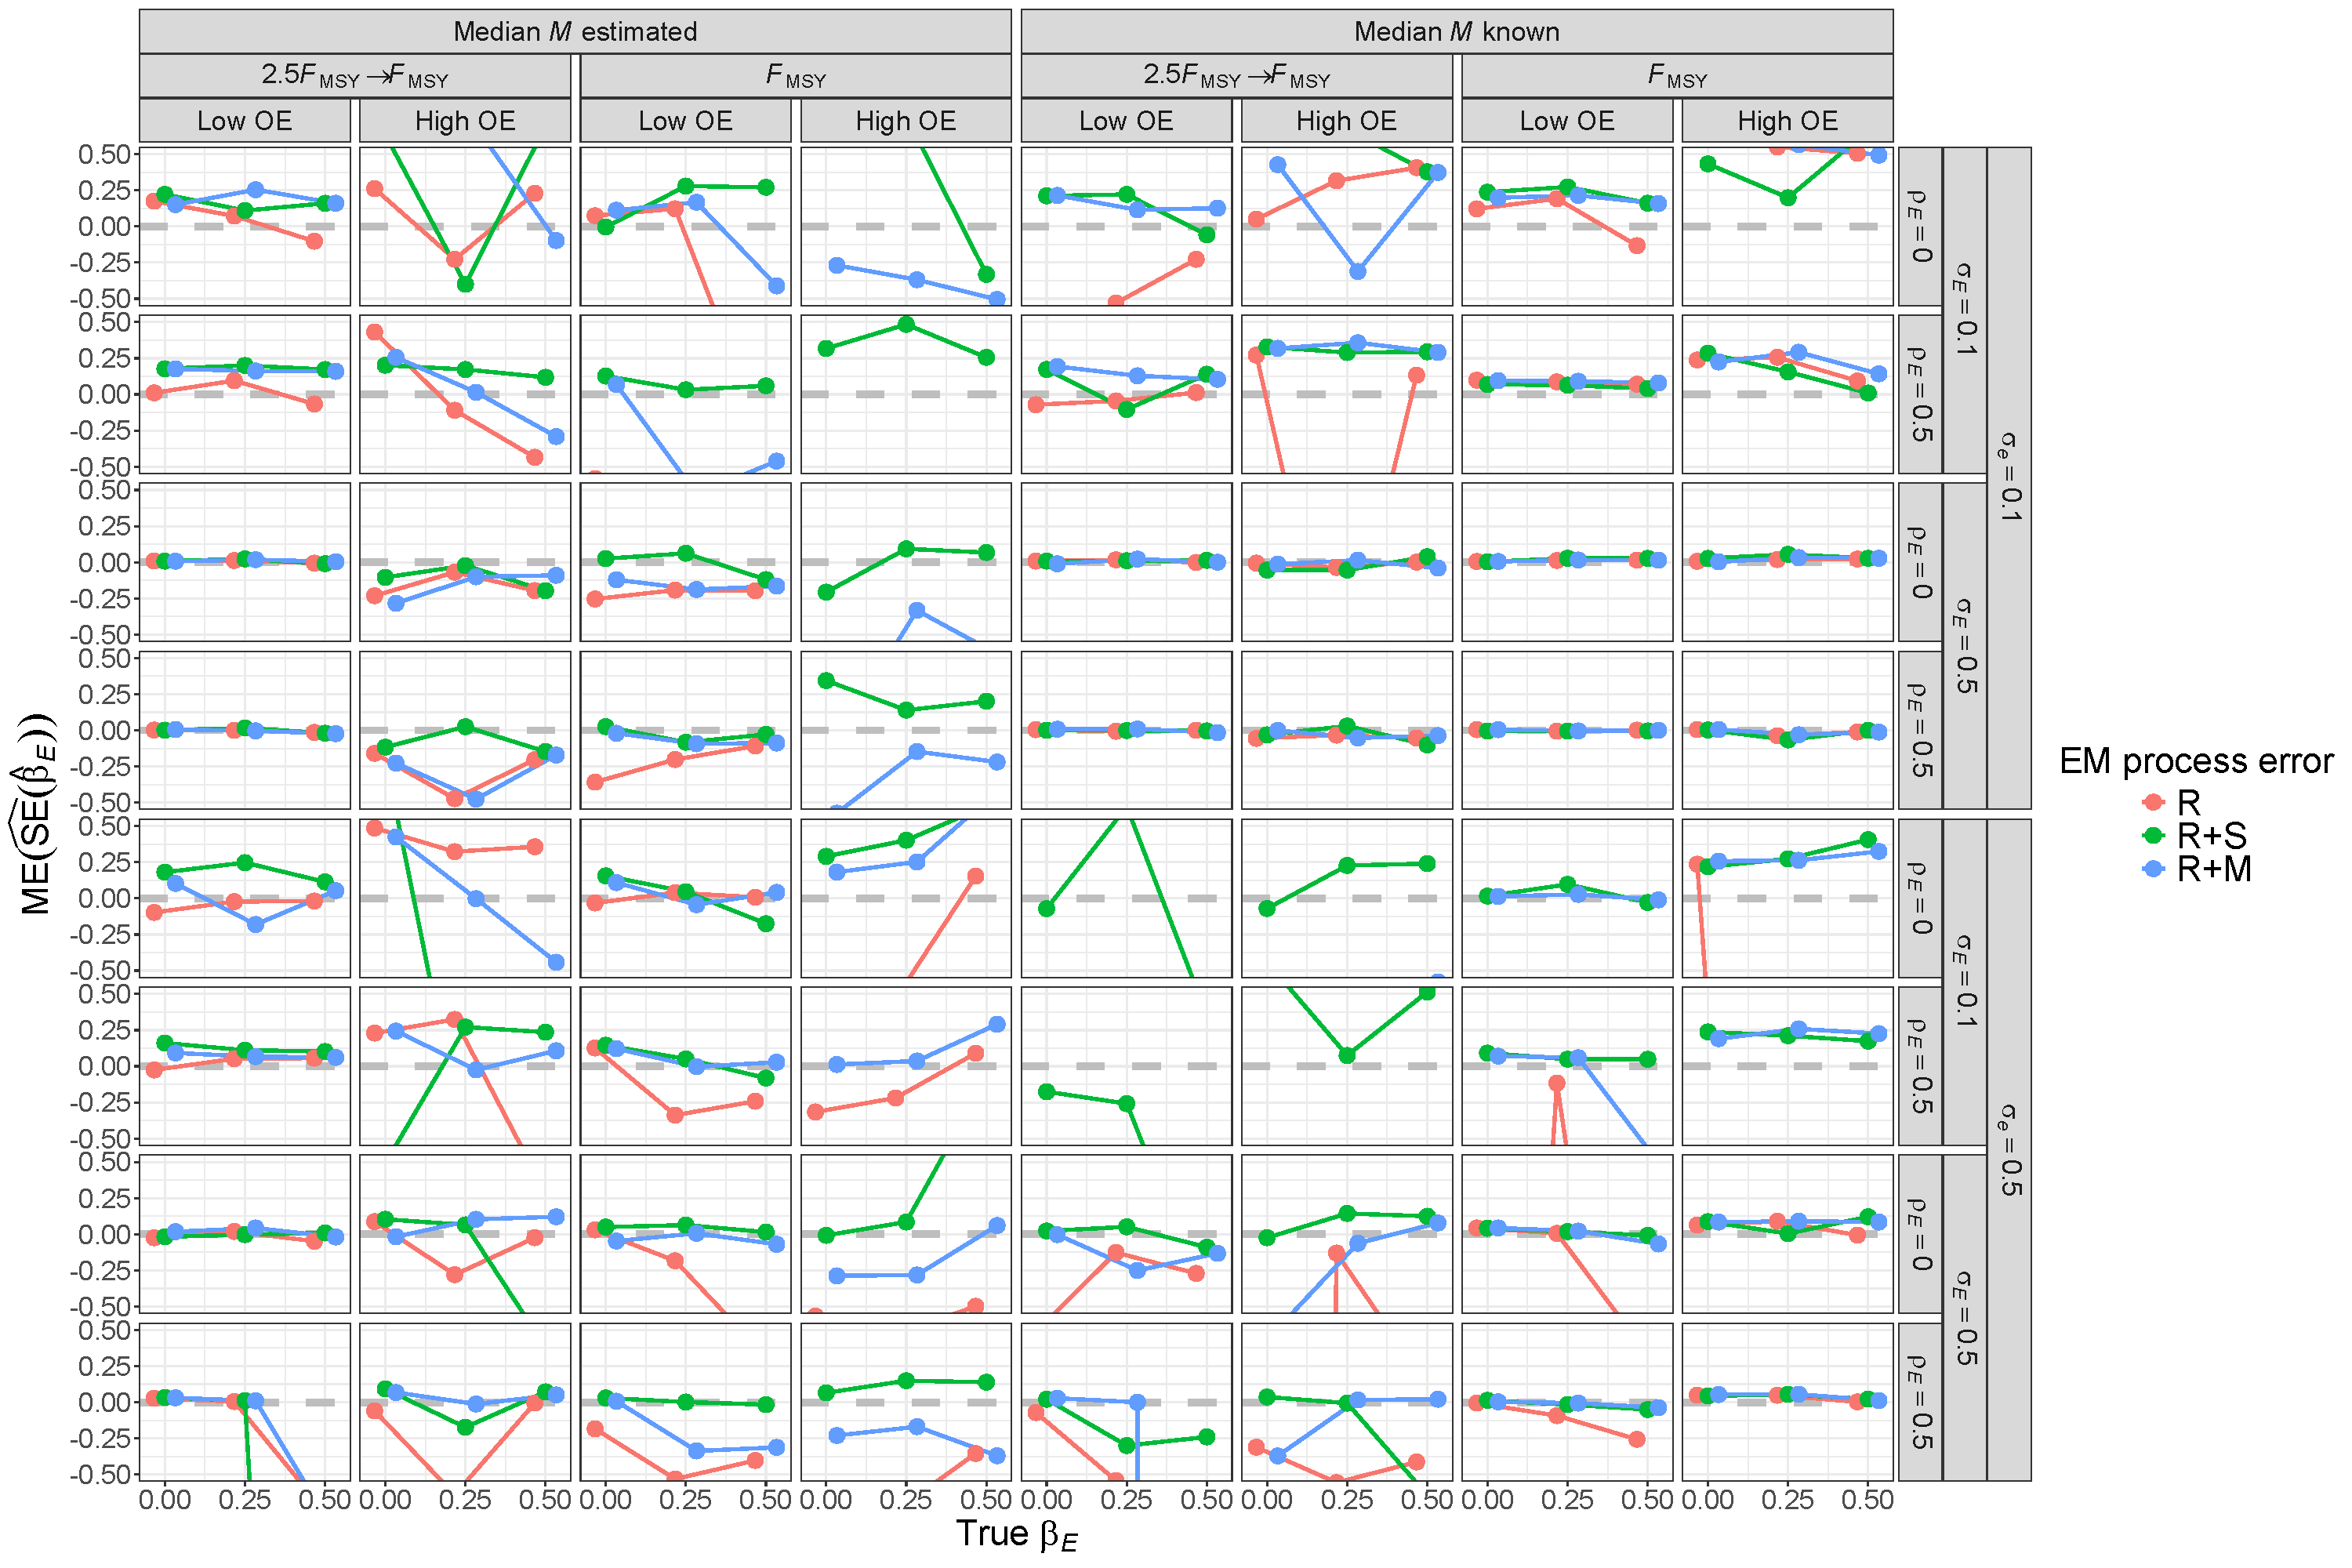
\includegraphics[height = \textheight]{se_beta_E_bias_Rom}
\end{center}
\caption{For R operating models, median error (ME) of Hessian-based estimates of standard error for covariate effect on $M$ ($\beta_E$) from fitting estimating models with alternative process error assumptions and treatment of median $M$ parameter ($\beta_M$). True standard error is defined as the mean of the standard error estimates accross converged fits to simulated data sets for a given operating model scenario.}\label{se_beta_E_bias_Rom}
\end{figure}
\end{landscape}

\begin{landscape}
\begin{figure}
\begin{center}
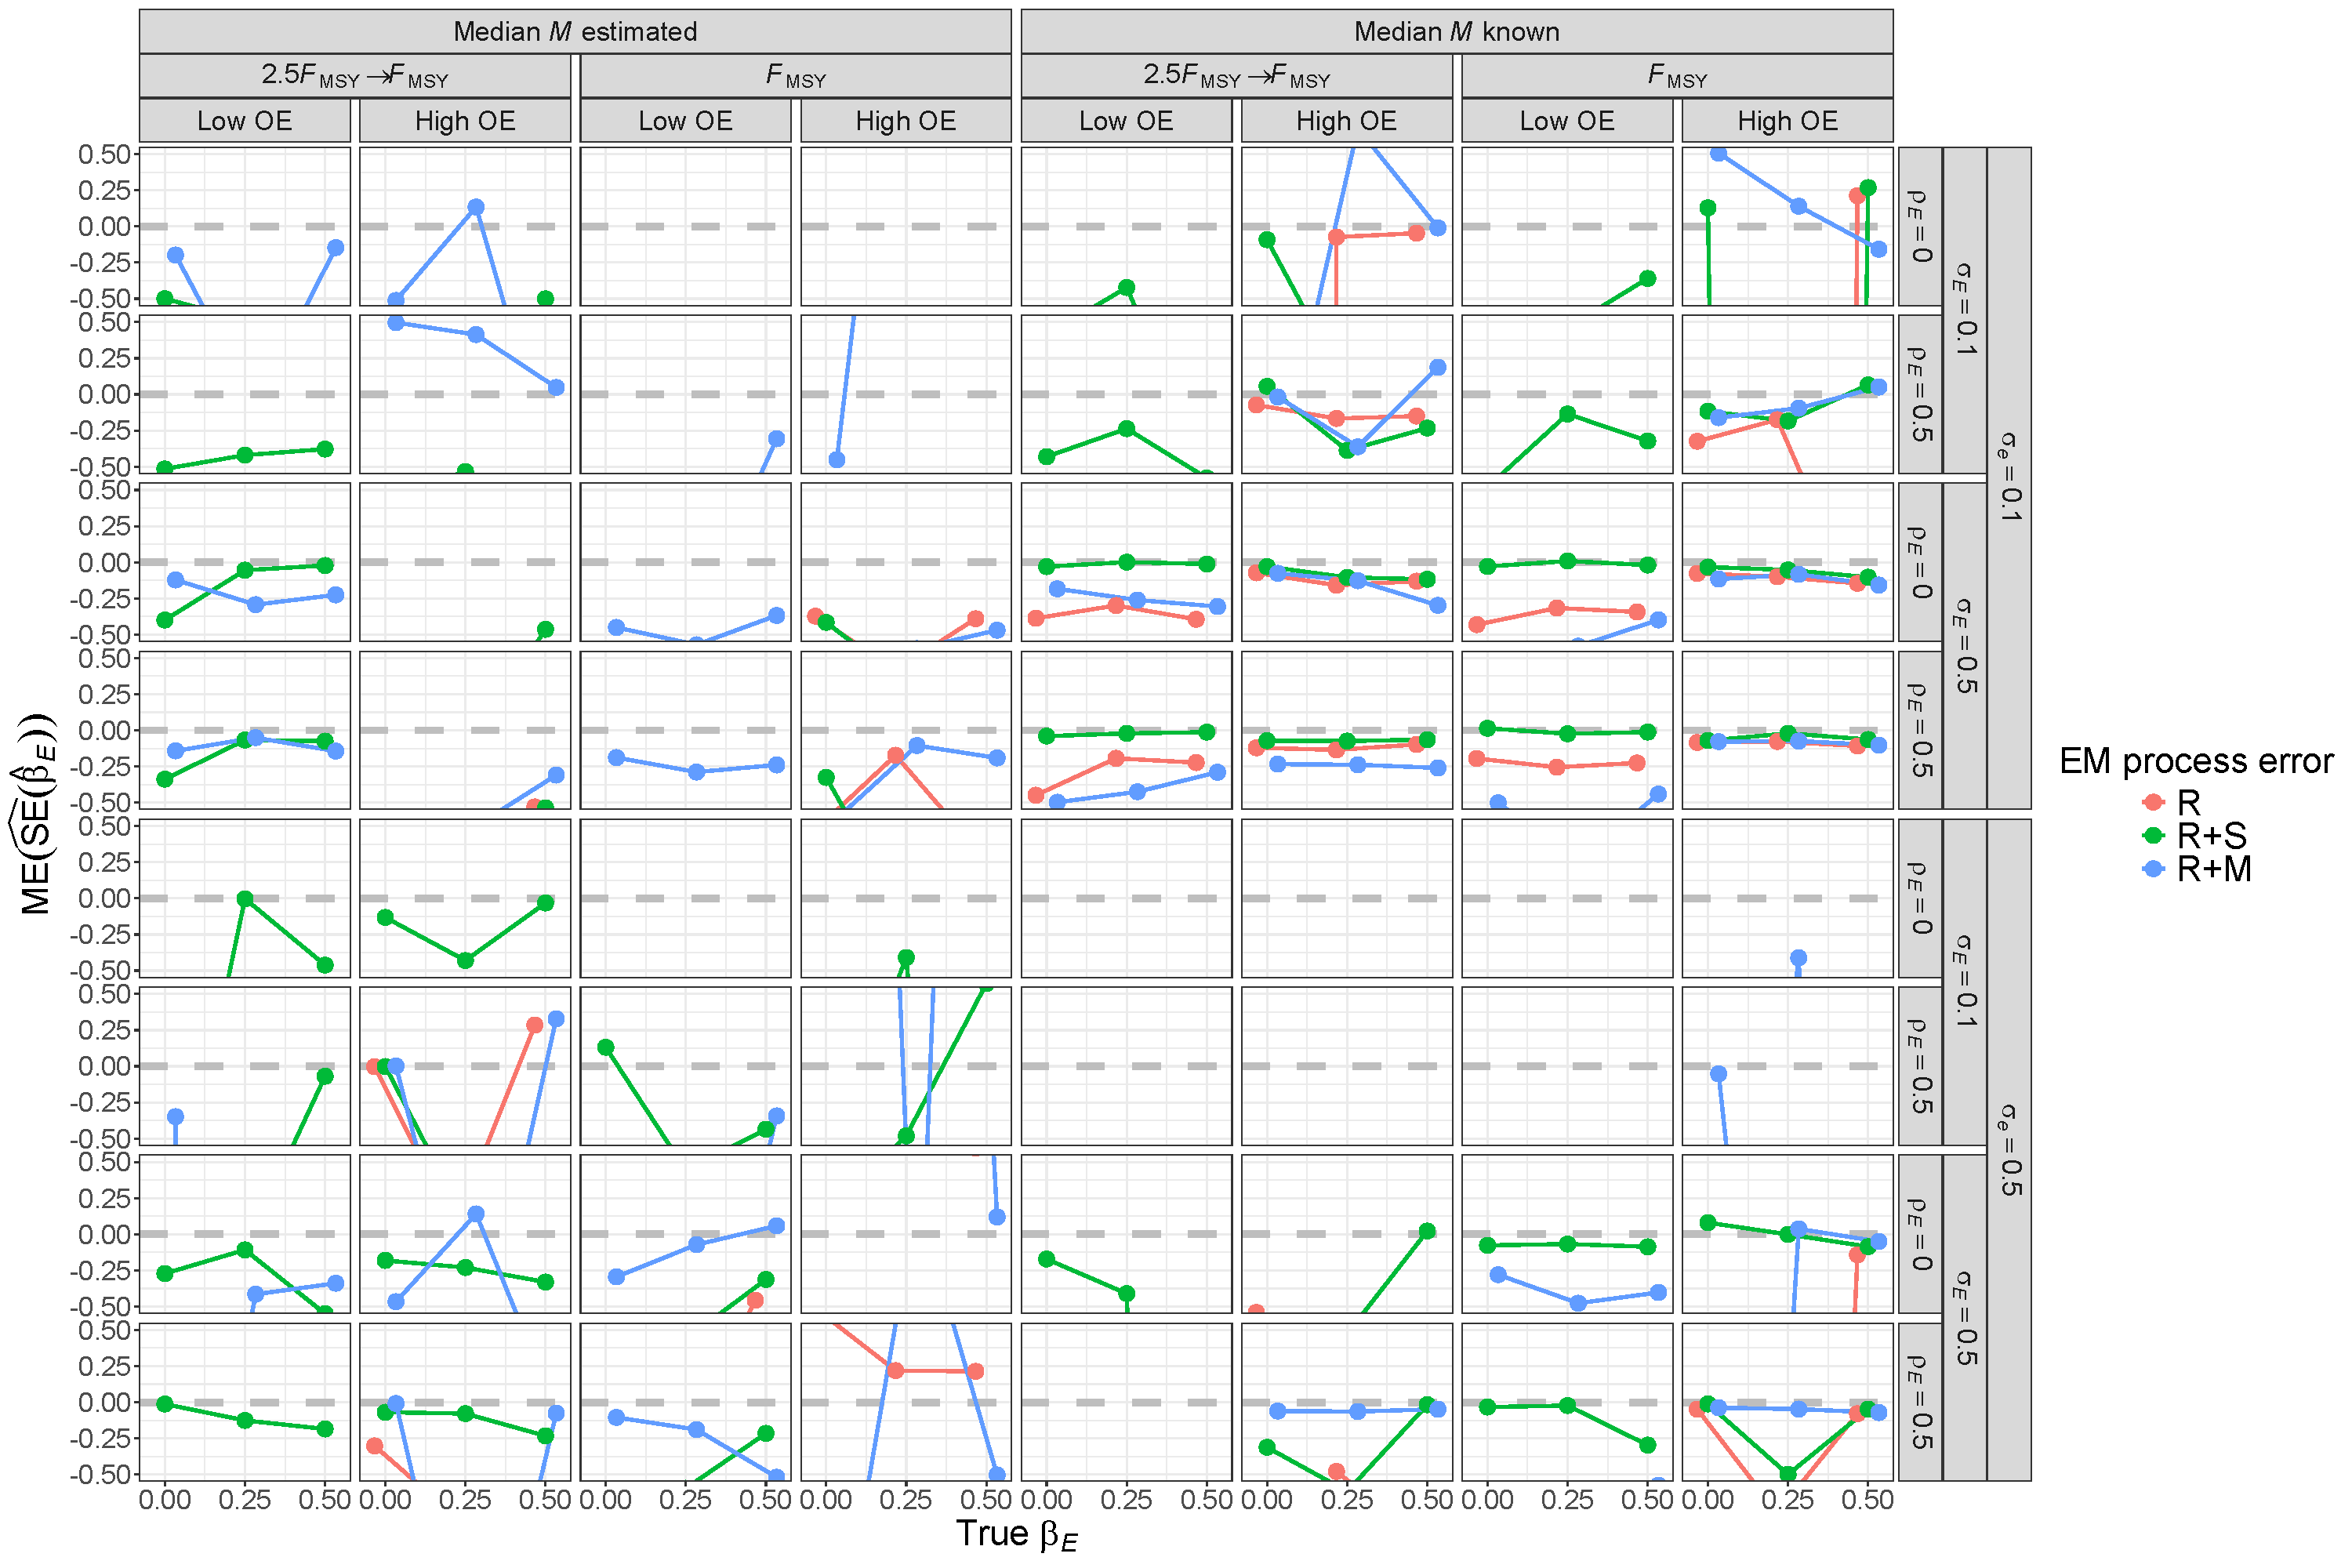
\includegraphics[height = \textheight]{se_beta_E_bias_RSom}
\end{center}
\caption{For R+S operating models, median error (ME) of Hessian-based estimates of standard error for covariate effect on $M$ ($\beta_E$) from fitting estimating models with alternative process error assumptions and treatment of median $M$ parameter ($\beta_M$). True standard error is defined as the mean of the standard error estimates accross converged fits to simulated data sets for a given operating model scenario.}\label{se_beta_E_bias_RSom}
\end{figure}
\end{landscape}

\begin{landscape}
\begin{figure}
\begin{center}
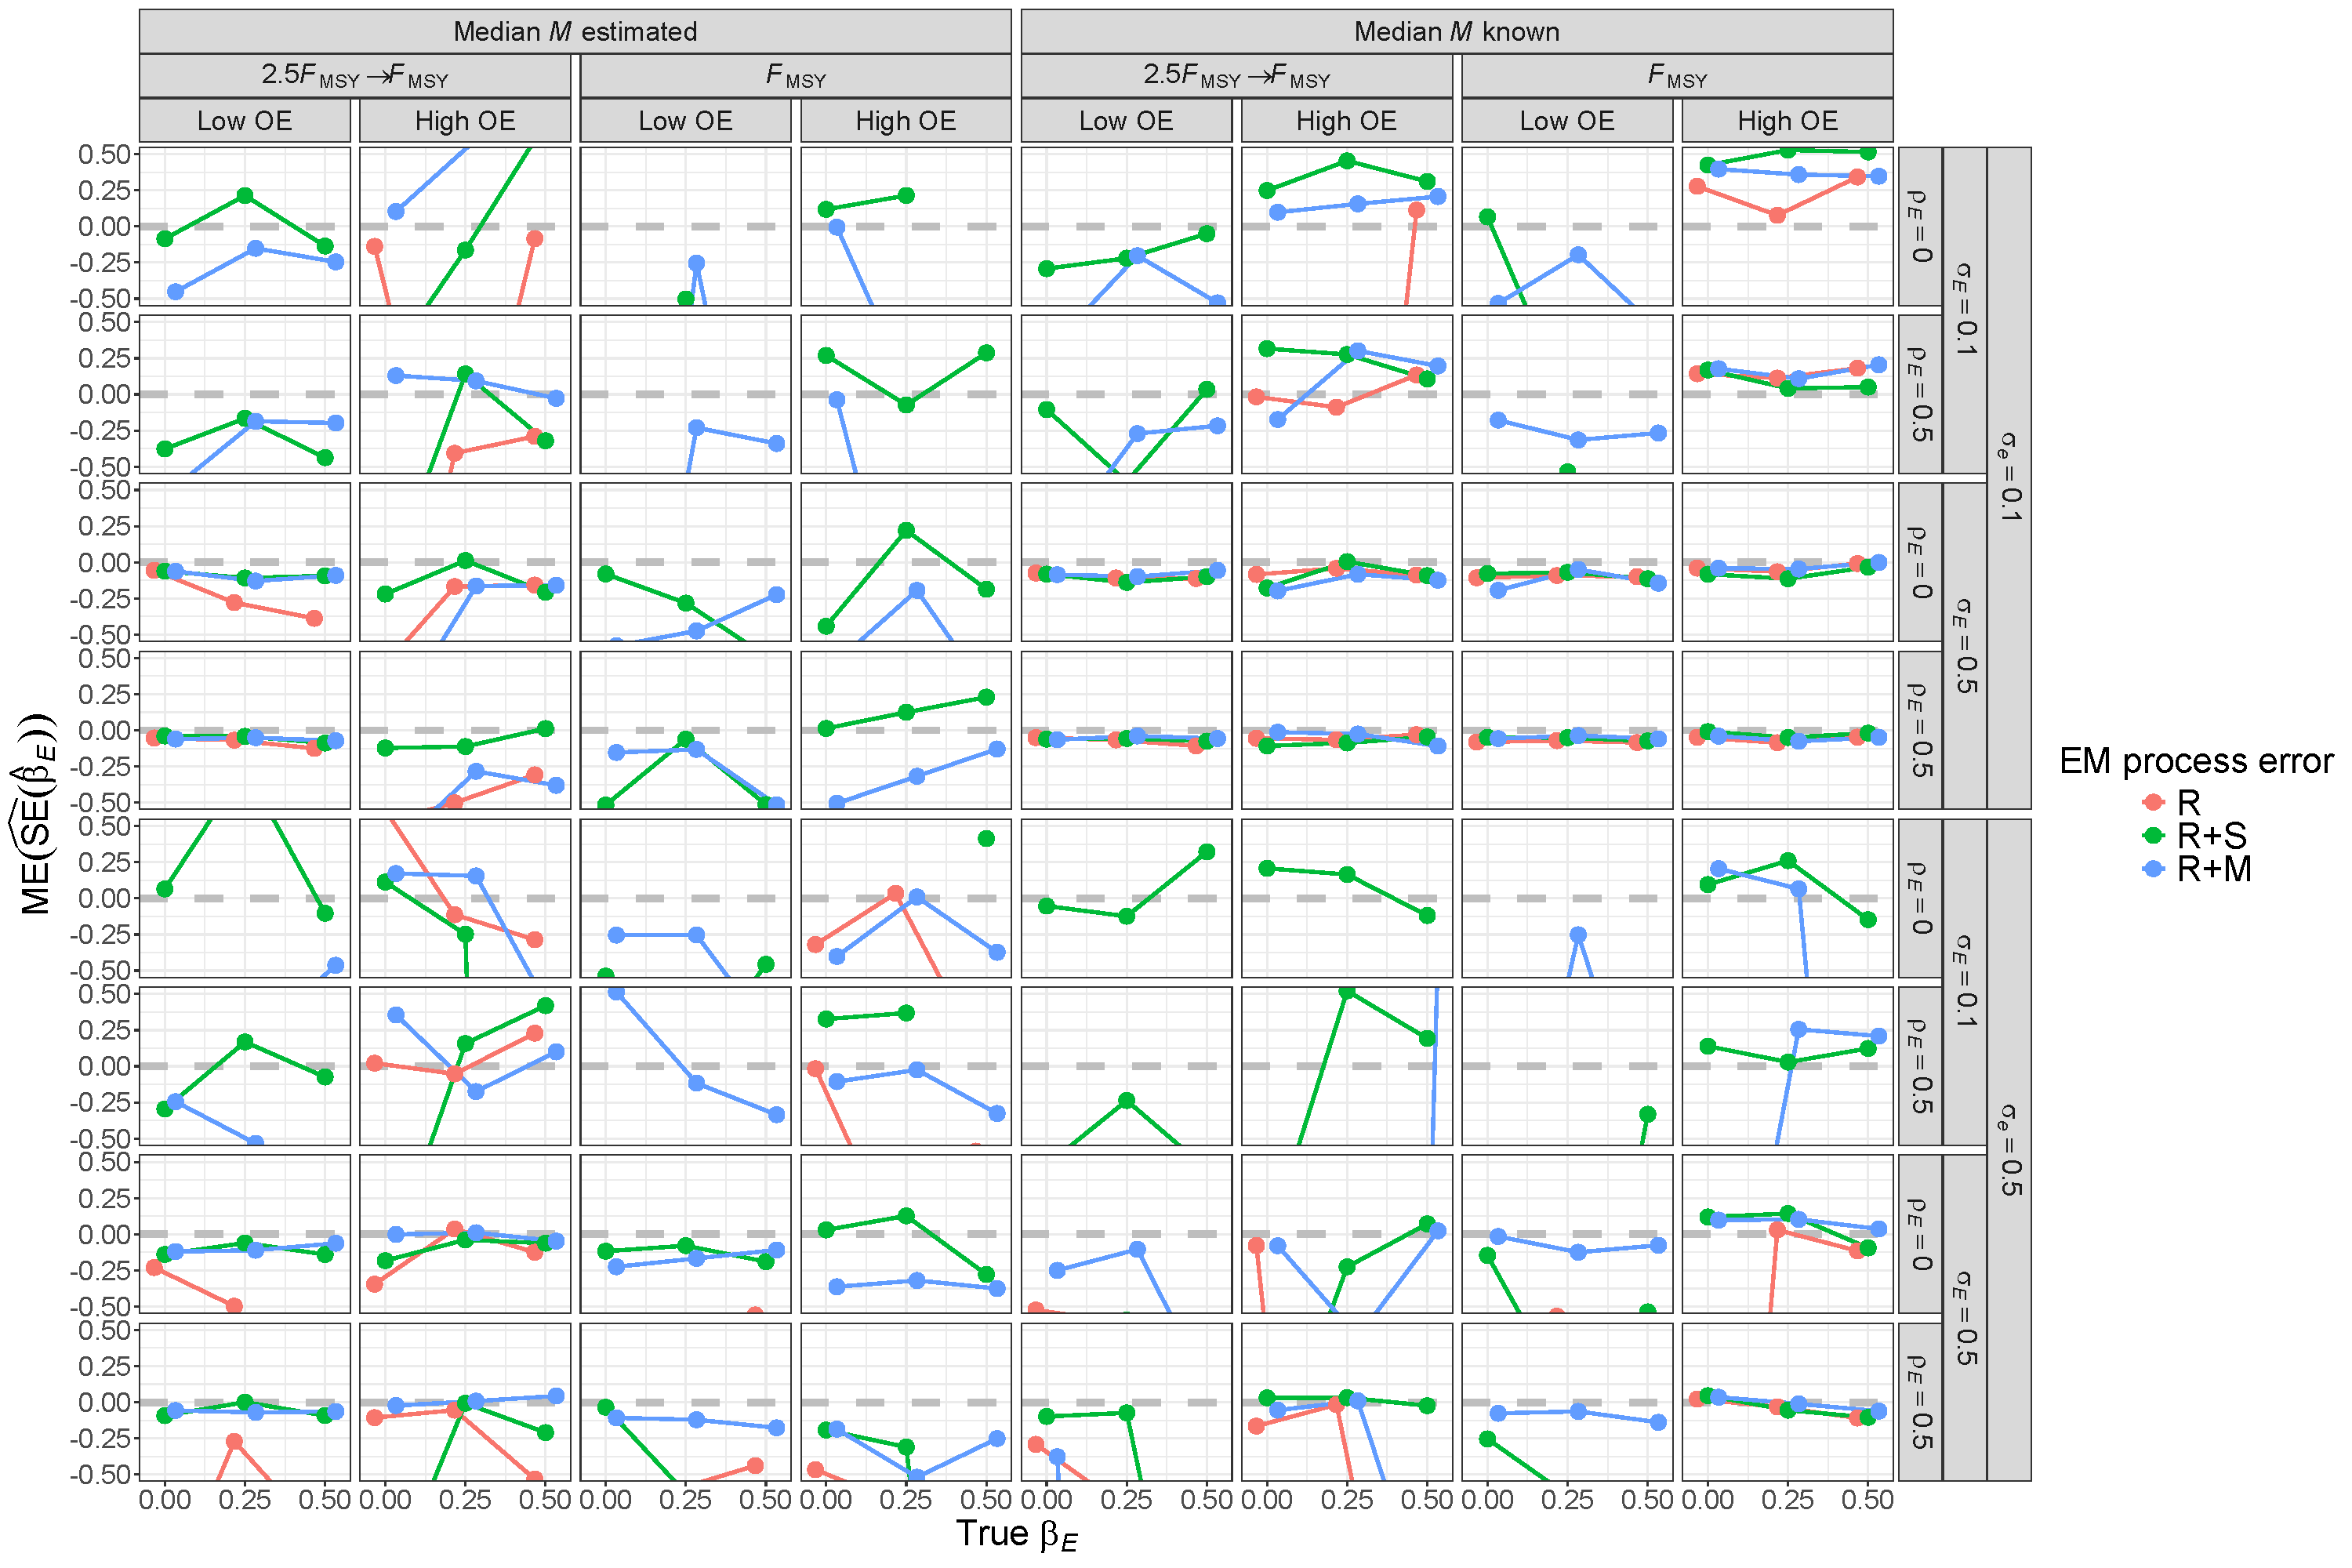
\includegraphics[height = \textheight]{se_beta_E_bias_RMom}
\end{center}
\caption{For R+M operating models, median error (ME) of Hessian-based estimates of standard error for covariate effect on $M$ ($\beta_E$) from fitting estimating models with alternative process error assumptions and treatment of median $M$ parameter ($\beta_M$). True standard error is defined as the mean of the standard error estimates accross converged fits to simulated data sets for a given operating model scenario.}\label{se_beta_E_bias_RMom}
\end{figure}
\end{landscape}

\begin{landscape}
\begin{figure}
\begin{center}
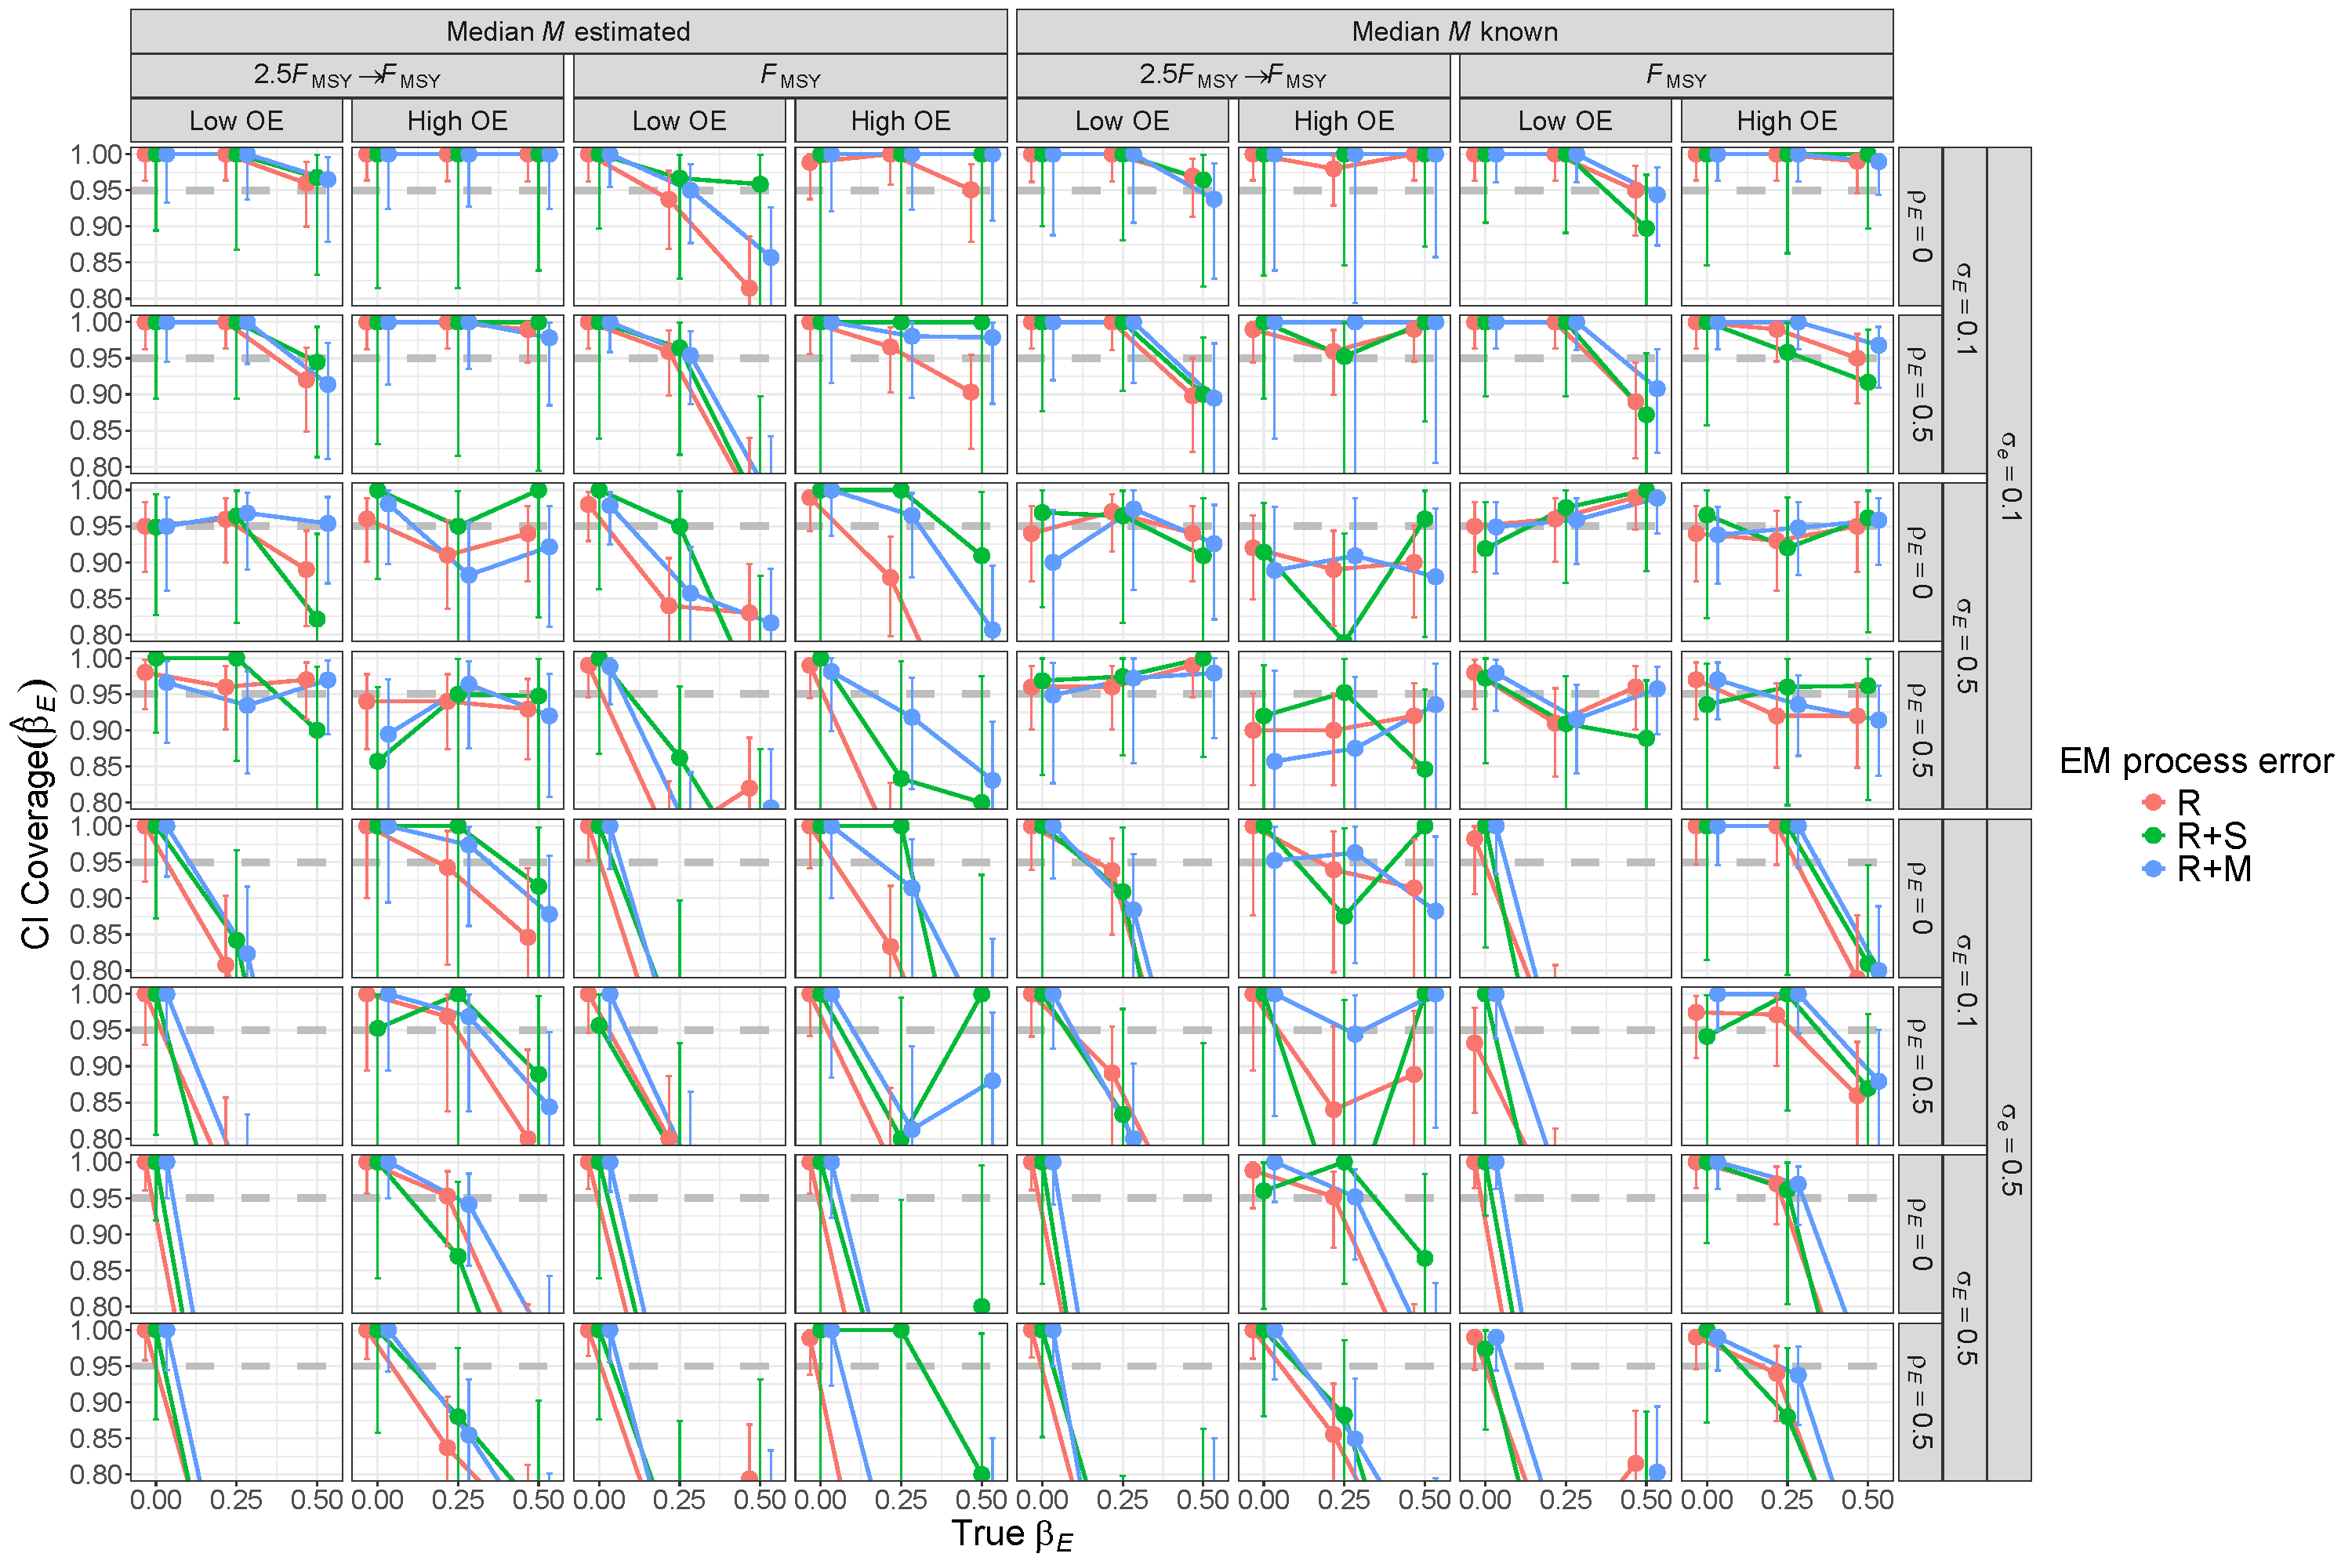
\includegraphics[height = \textheight]{beta_E_CI_coverage_Rom}
\end{center}
\caption{For R operating models, probability of 95\% confidence interval for $\beta_E$ containing the true value for estimating models with alternative process error assumptions and treatment of median $M$ parameter ($\beta_M$). Vertical lines represent 95\% confidence intervals.}\label{beta_E_CI_coverage_Rom}
\end{figure}
\end{landscape}

\begin{landscape}
\begin{figure}
\begin{center}
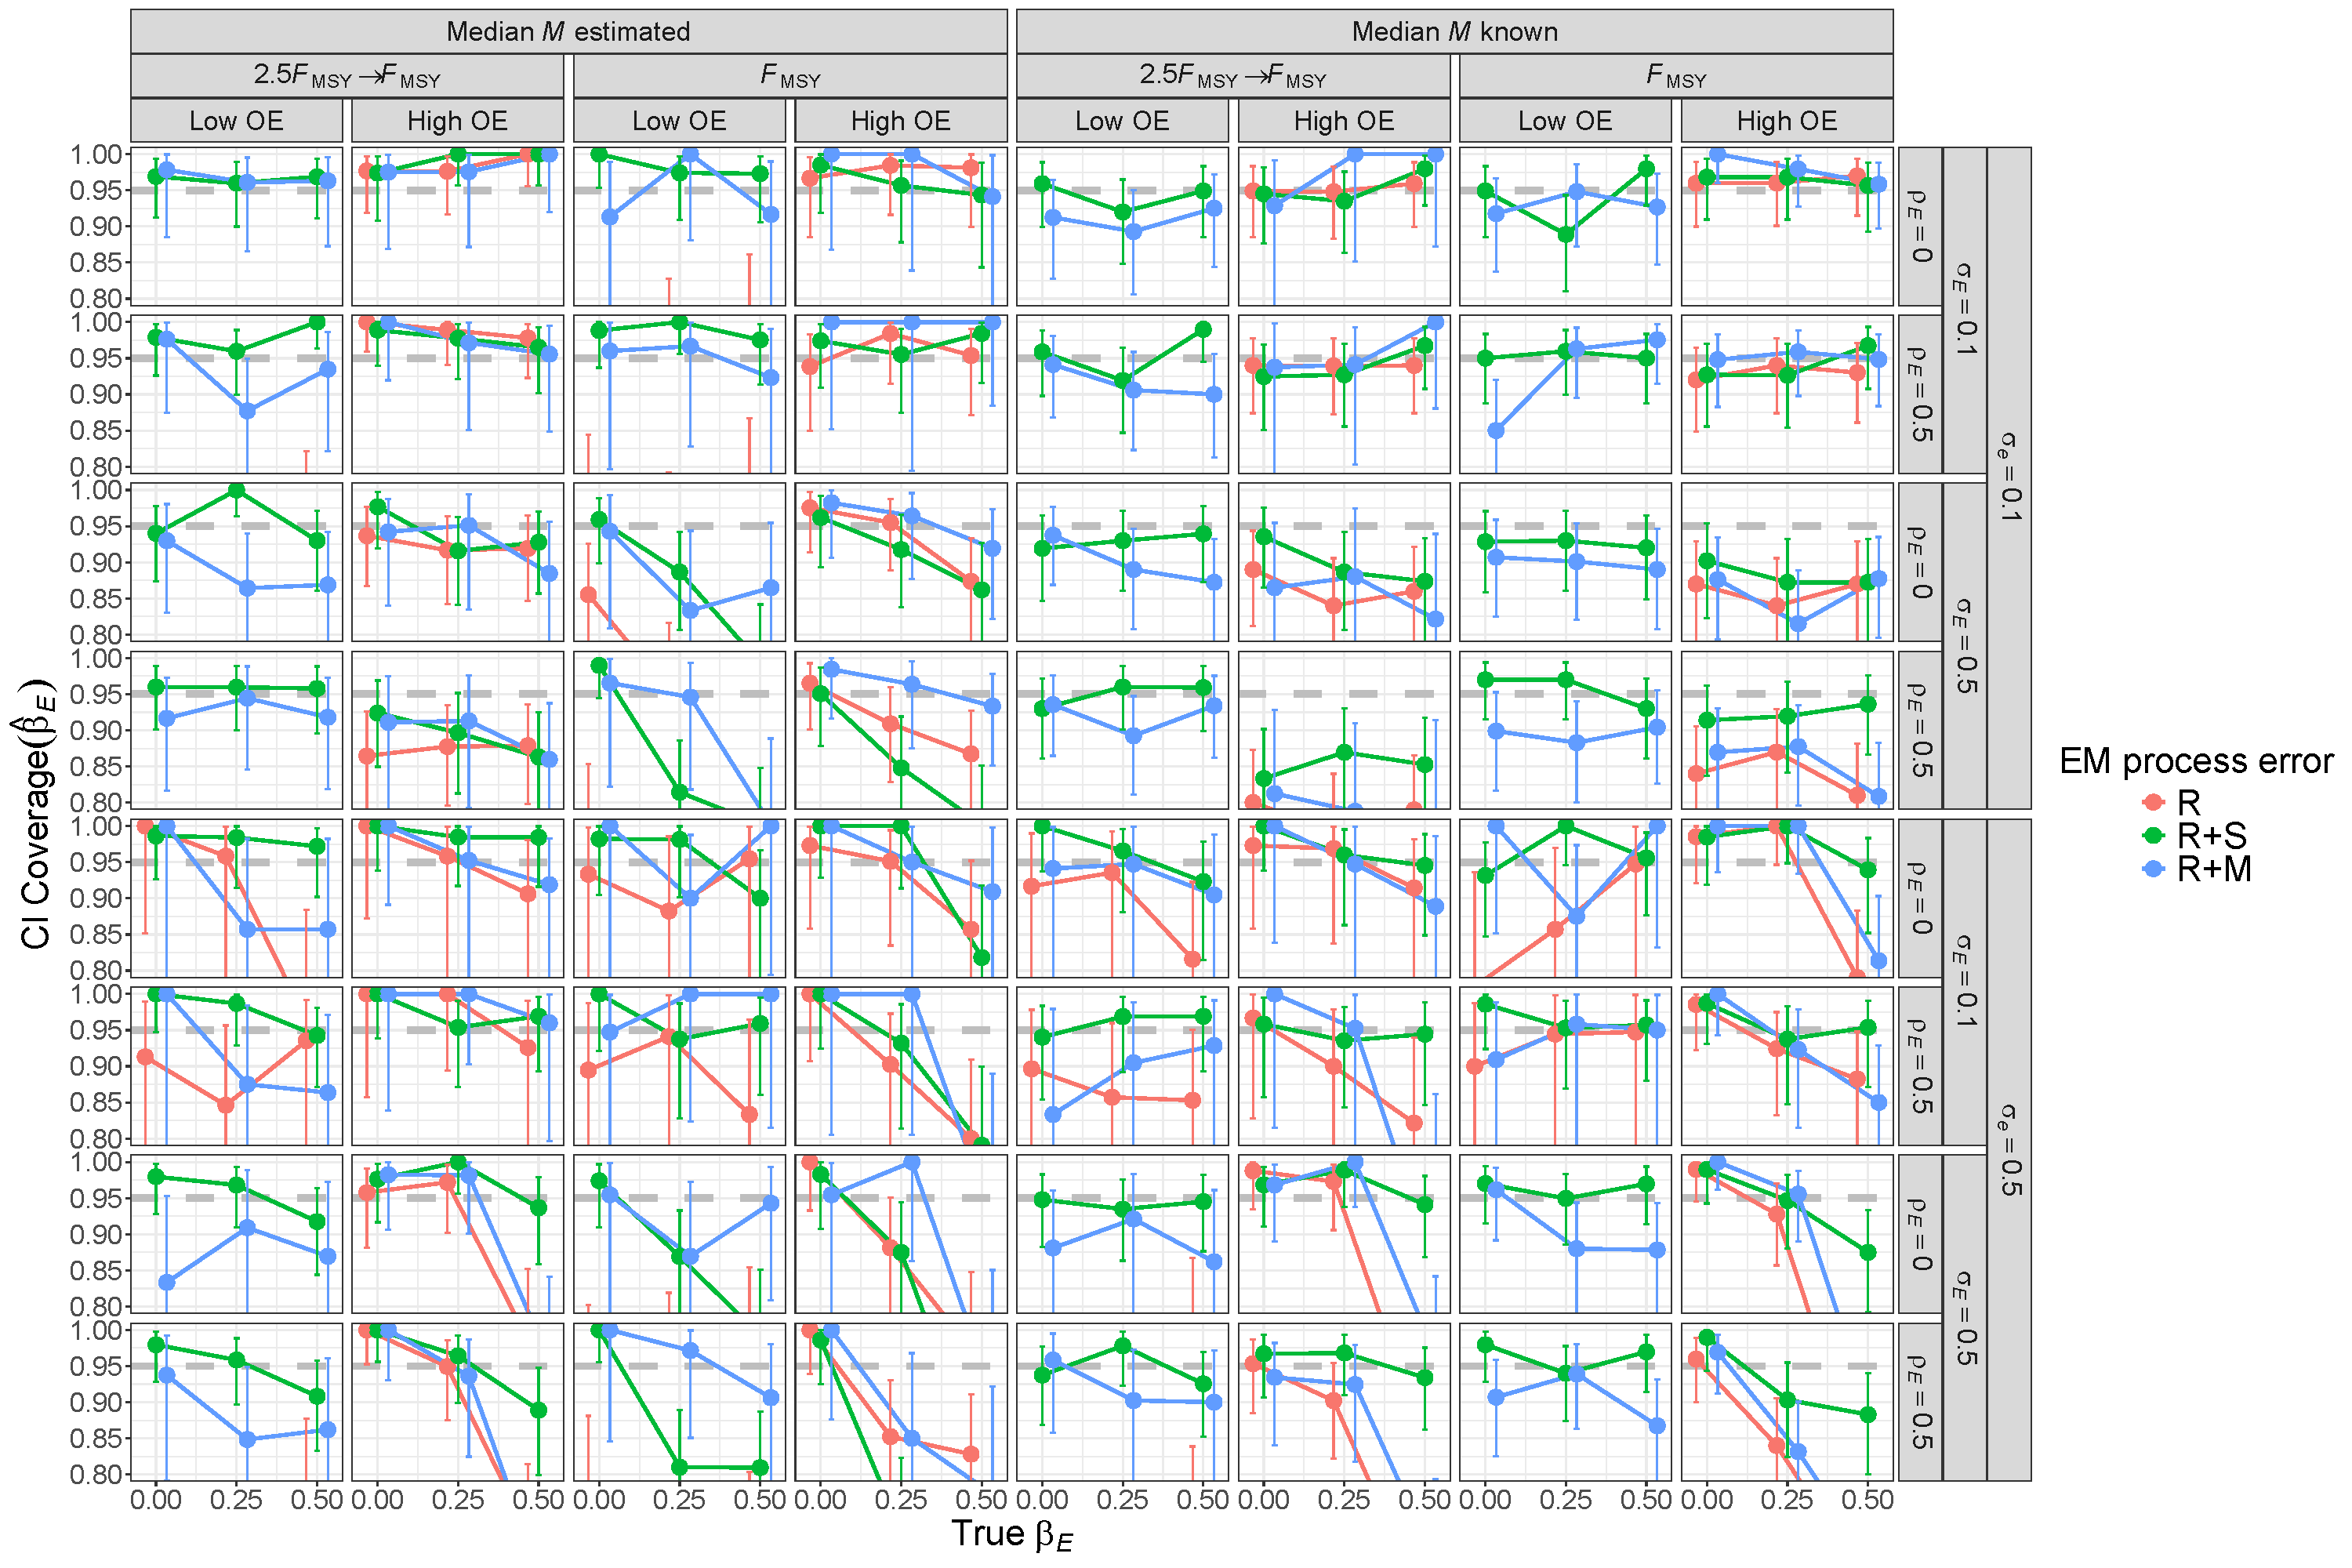
\includegraphics[height = \textheight]{beta_E_CI_coverage_RSom}
\end{center}
\caption{For R+S operating models, probability of 95\% confidence interval for $\beta_E$ containing the true value for estimating models with alternative process error assumptions and treatment of median $M$ parameter ($\beta_M$). Vertical lines represent 95\% confidence intervals.}\label{beta_E_CI_coverage_RSom}
\end{figure}
\end{landscape}

\begin{landscape}
\begin{figure}
\begin{center}
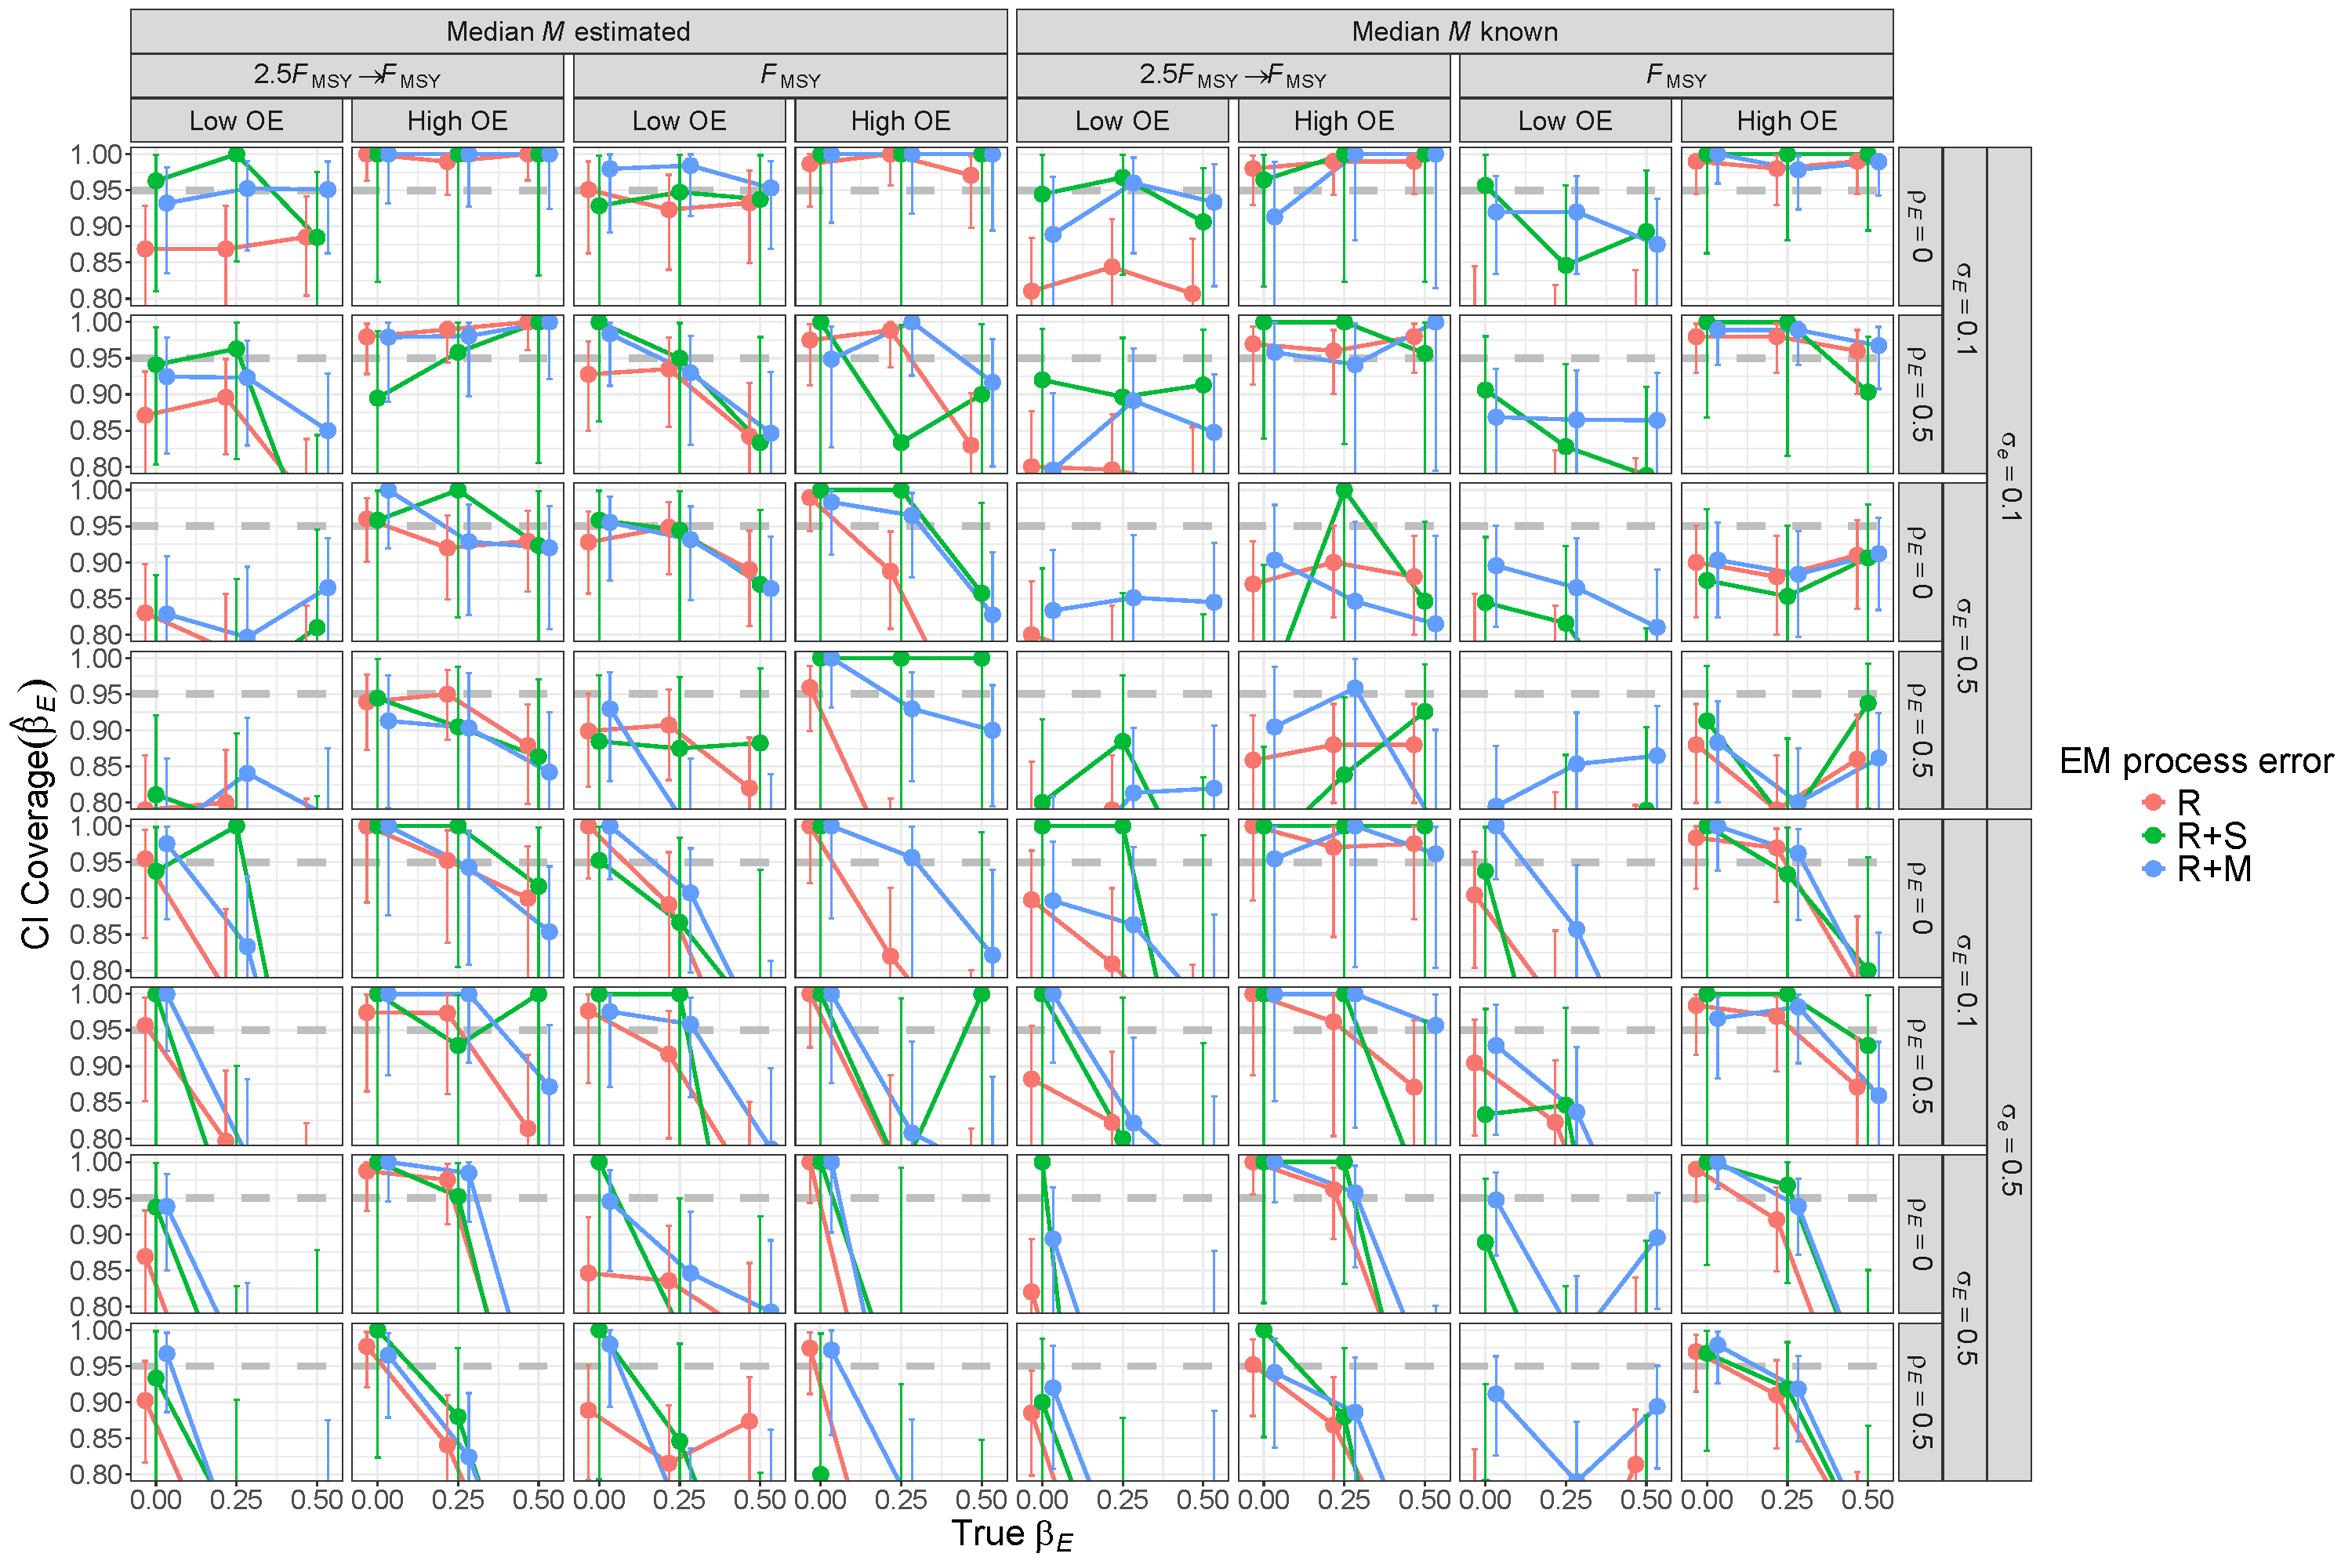
\includegraphics[height = \textheight]{beta_E_CI_coverage_RMom}
\end{center}
\caption{For R+M operating models, probability of 95\% confidence interval for $\beta_E$ containing the true value for estimating models with alternative process error assumptions and treatment of median $M$ parameter ($\beta_M$). Vertical lines represent 95\% confidence intervals.}\label{beta_E_CI_coverage_RMom}
\end{figure}
\end{landscape}

\begin{landscape}
\begin{figure}
\begin{center}
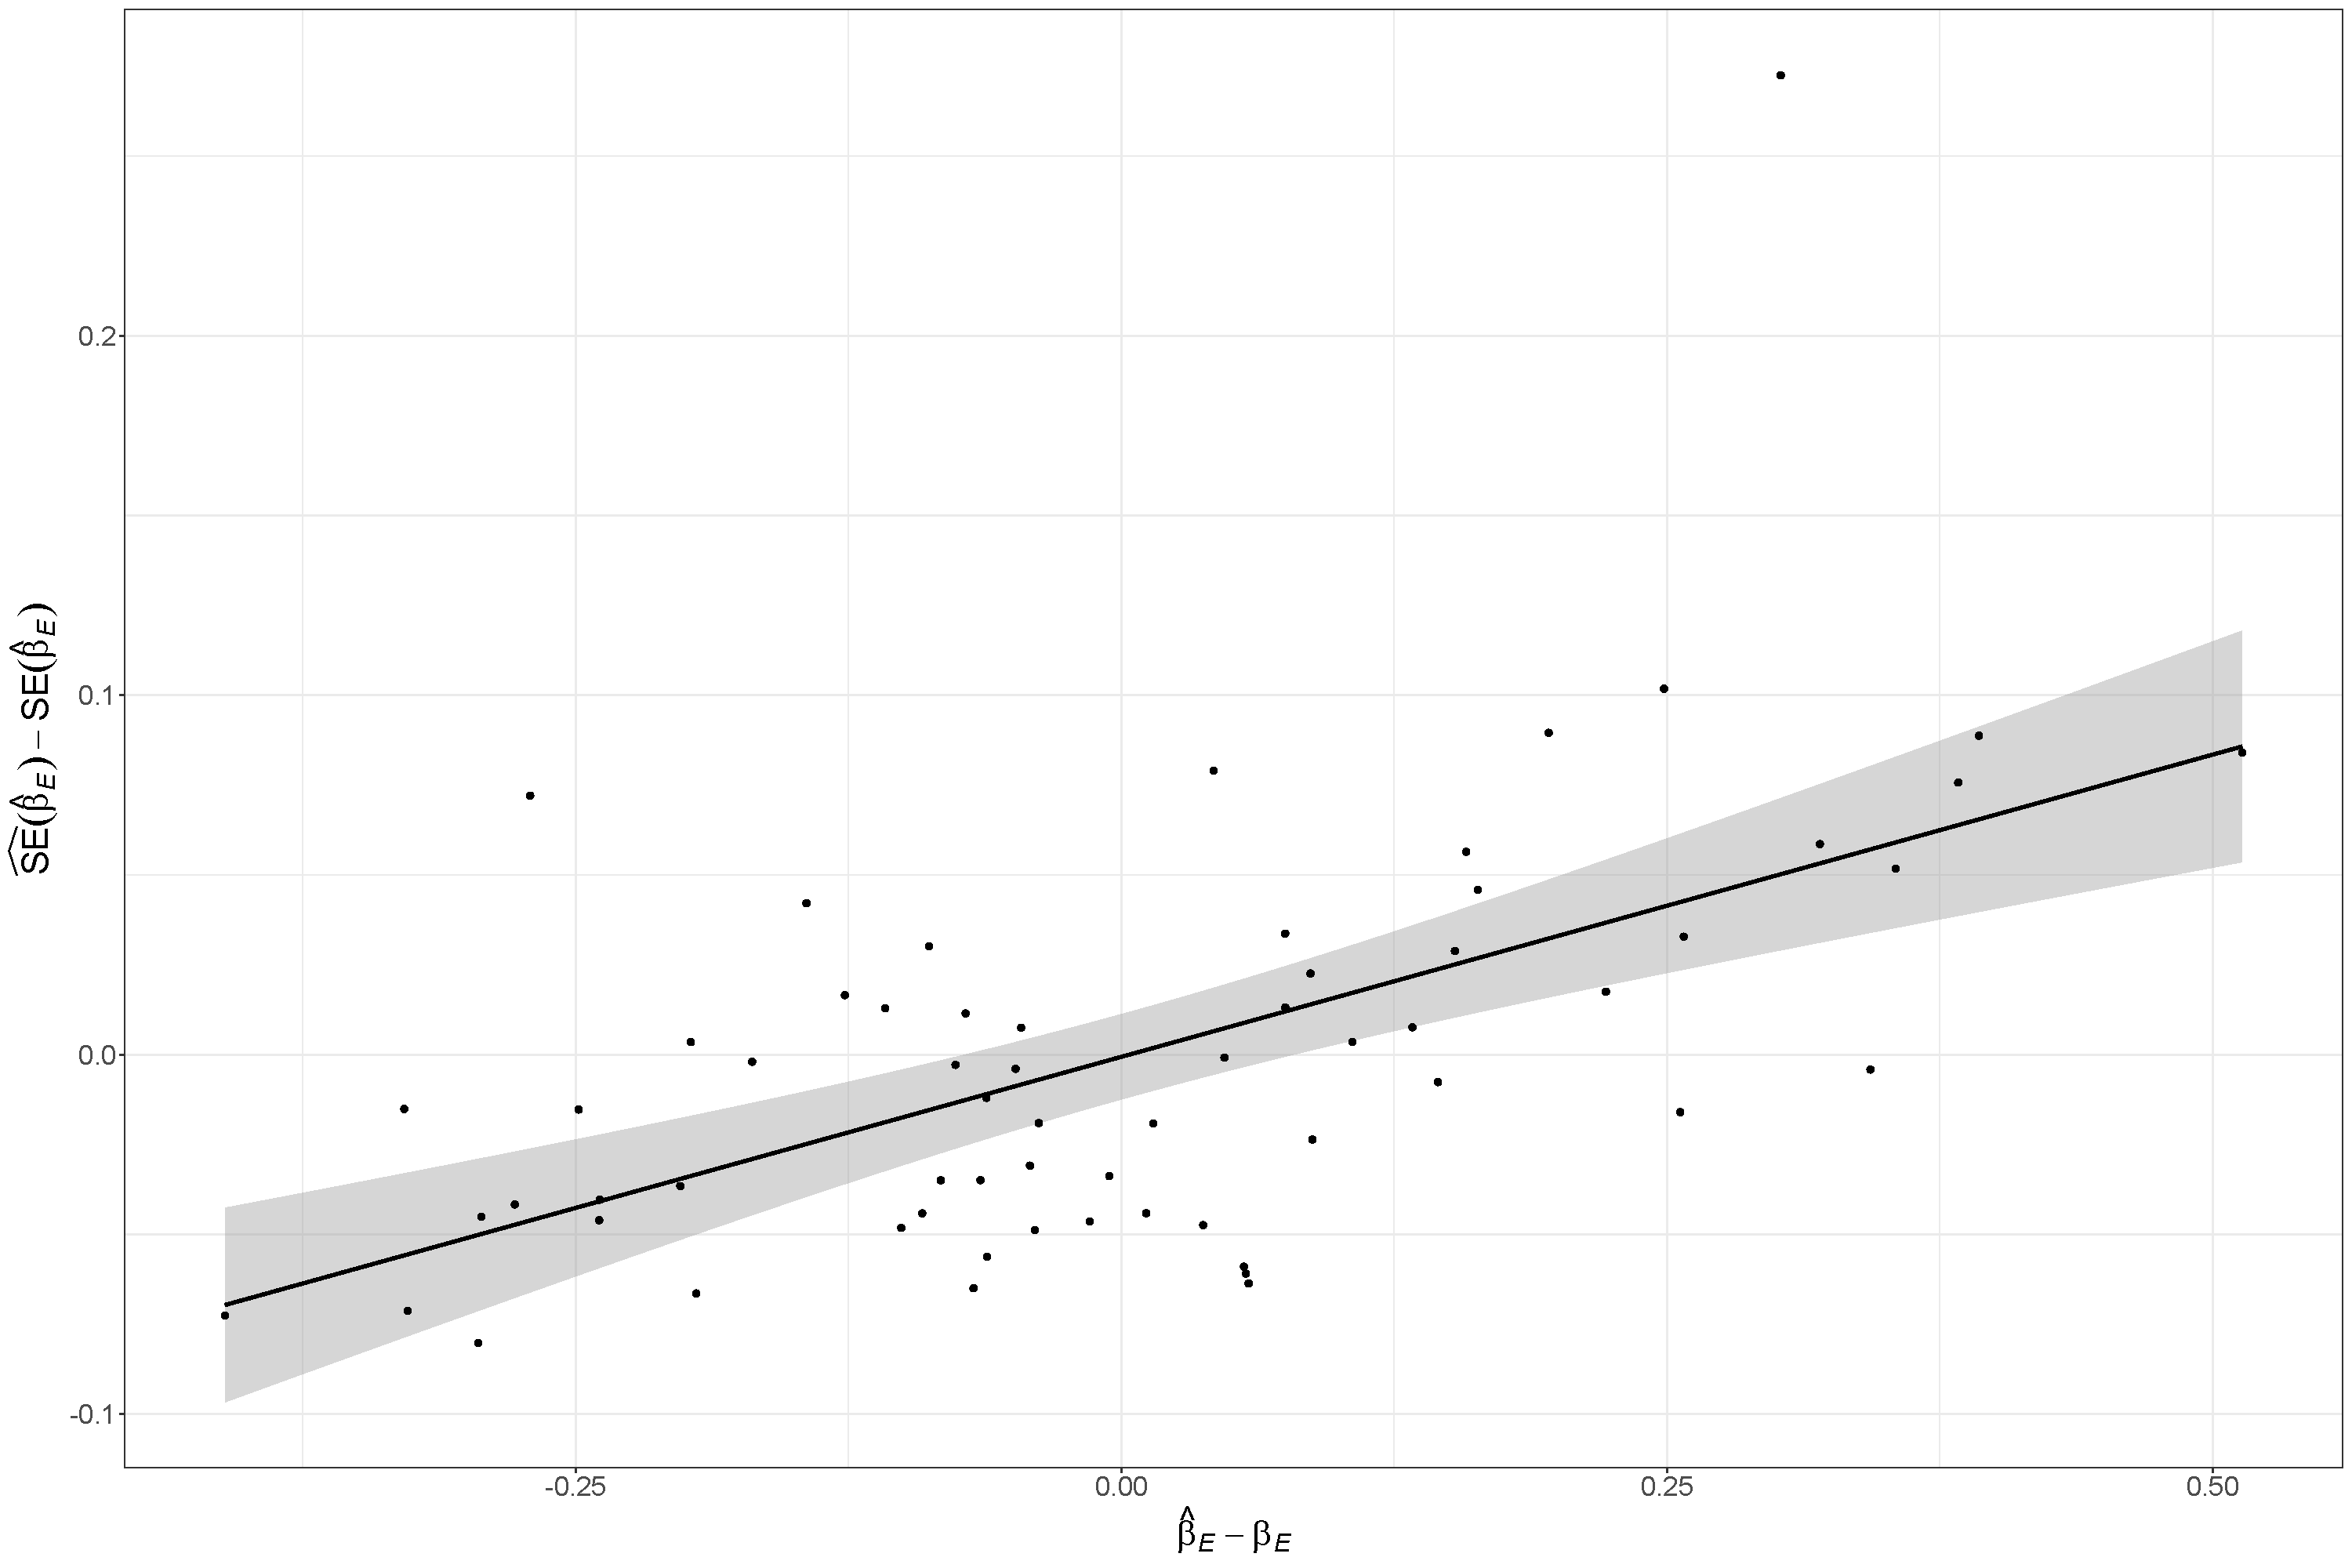
\includegraphics[height = 0.9\textheight]{om_69_em_5_beta_E_se_beta_E_lm_plot}
\end{center}
\caption{Positive correlation of covariate effect estimates and Hessian-based standard error estimates for estimating model that also estimates the median $M$ parameter ($\beta_M$) and has correct R+M process error assumption fitted to simulated data from the operating model with R+M process errors, temporal contrast in fishing pressure, low observation uncertainty for both population ($Low OE$) and covariate observations ($\sigma_e = 0.1$), high and uncorrelated temporal variability in the true covariate ($\sigma_E = 0.5$ and $\rho_E = 0$), and the strongest covariate effect on $M$ ($\beta_E = 0.5$).}\label{ex_lm_beta_E_SE_beta_E}
\end{figure}
\end{landscape}

\begin{landscape}
\begin{figure}
\begin{center}
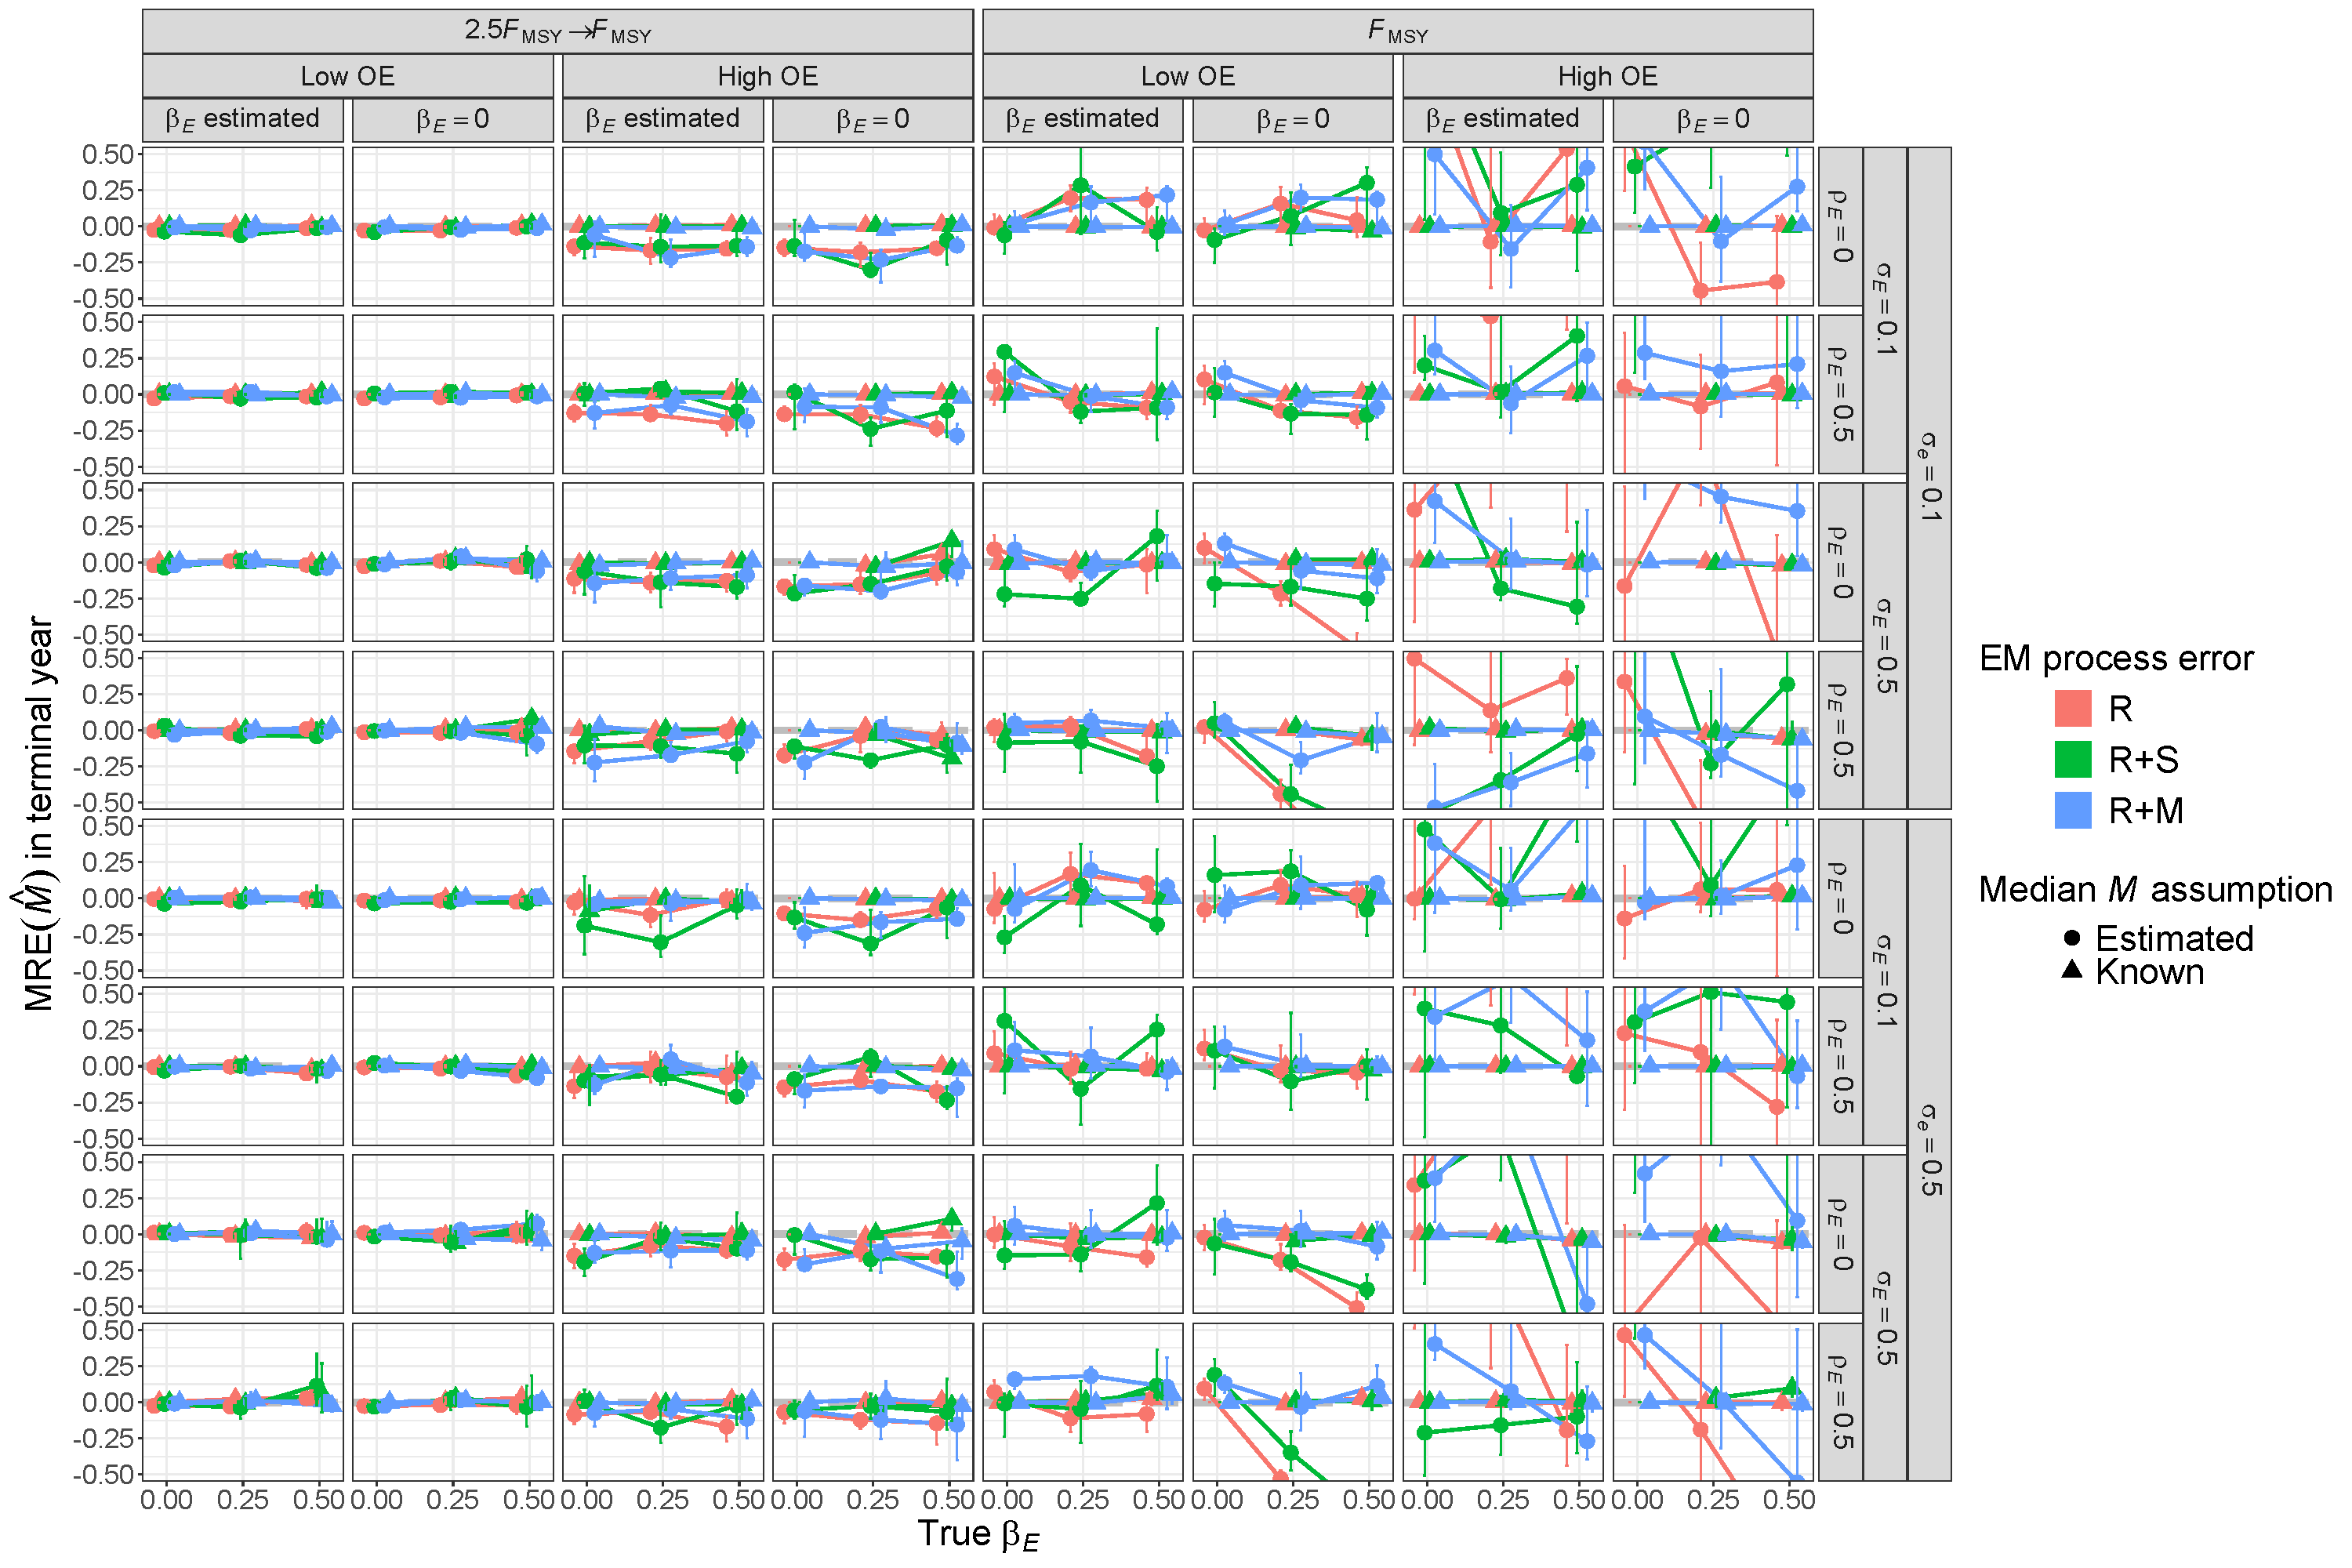
\includegraphics[height = \textheight]{terminal_year_M_bias_Rom}
\end{center}
\caption{For R operating models, median relative error (MRE) of estimates of terminal year $M$ for estimating models with alternative process error assumptions, treatment of covariate effect ($\beta_E = 0$ or estimated), and treatment of median $M$ parameter ($\beta_M$ estimated or known).}\label{terminal_M_bias_Rom}
\end{figure}
\end{landscape}

\begin{landscape}
\begin{figure}
\begin{center}
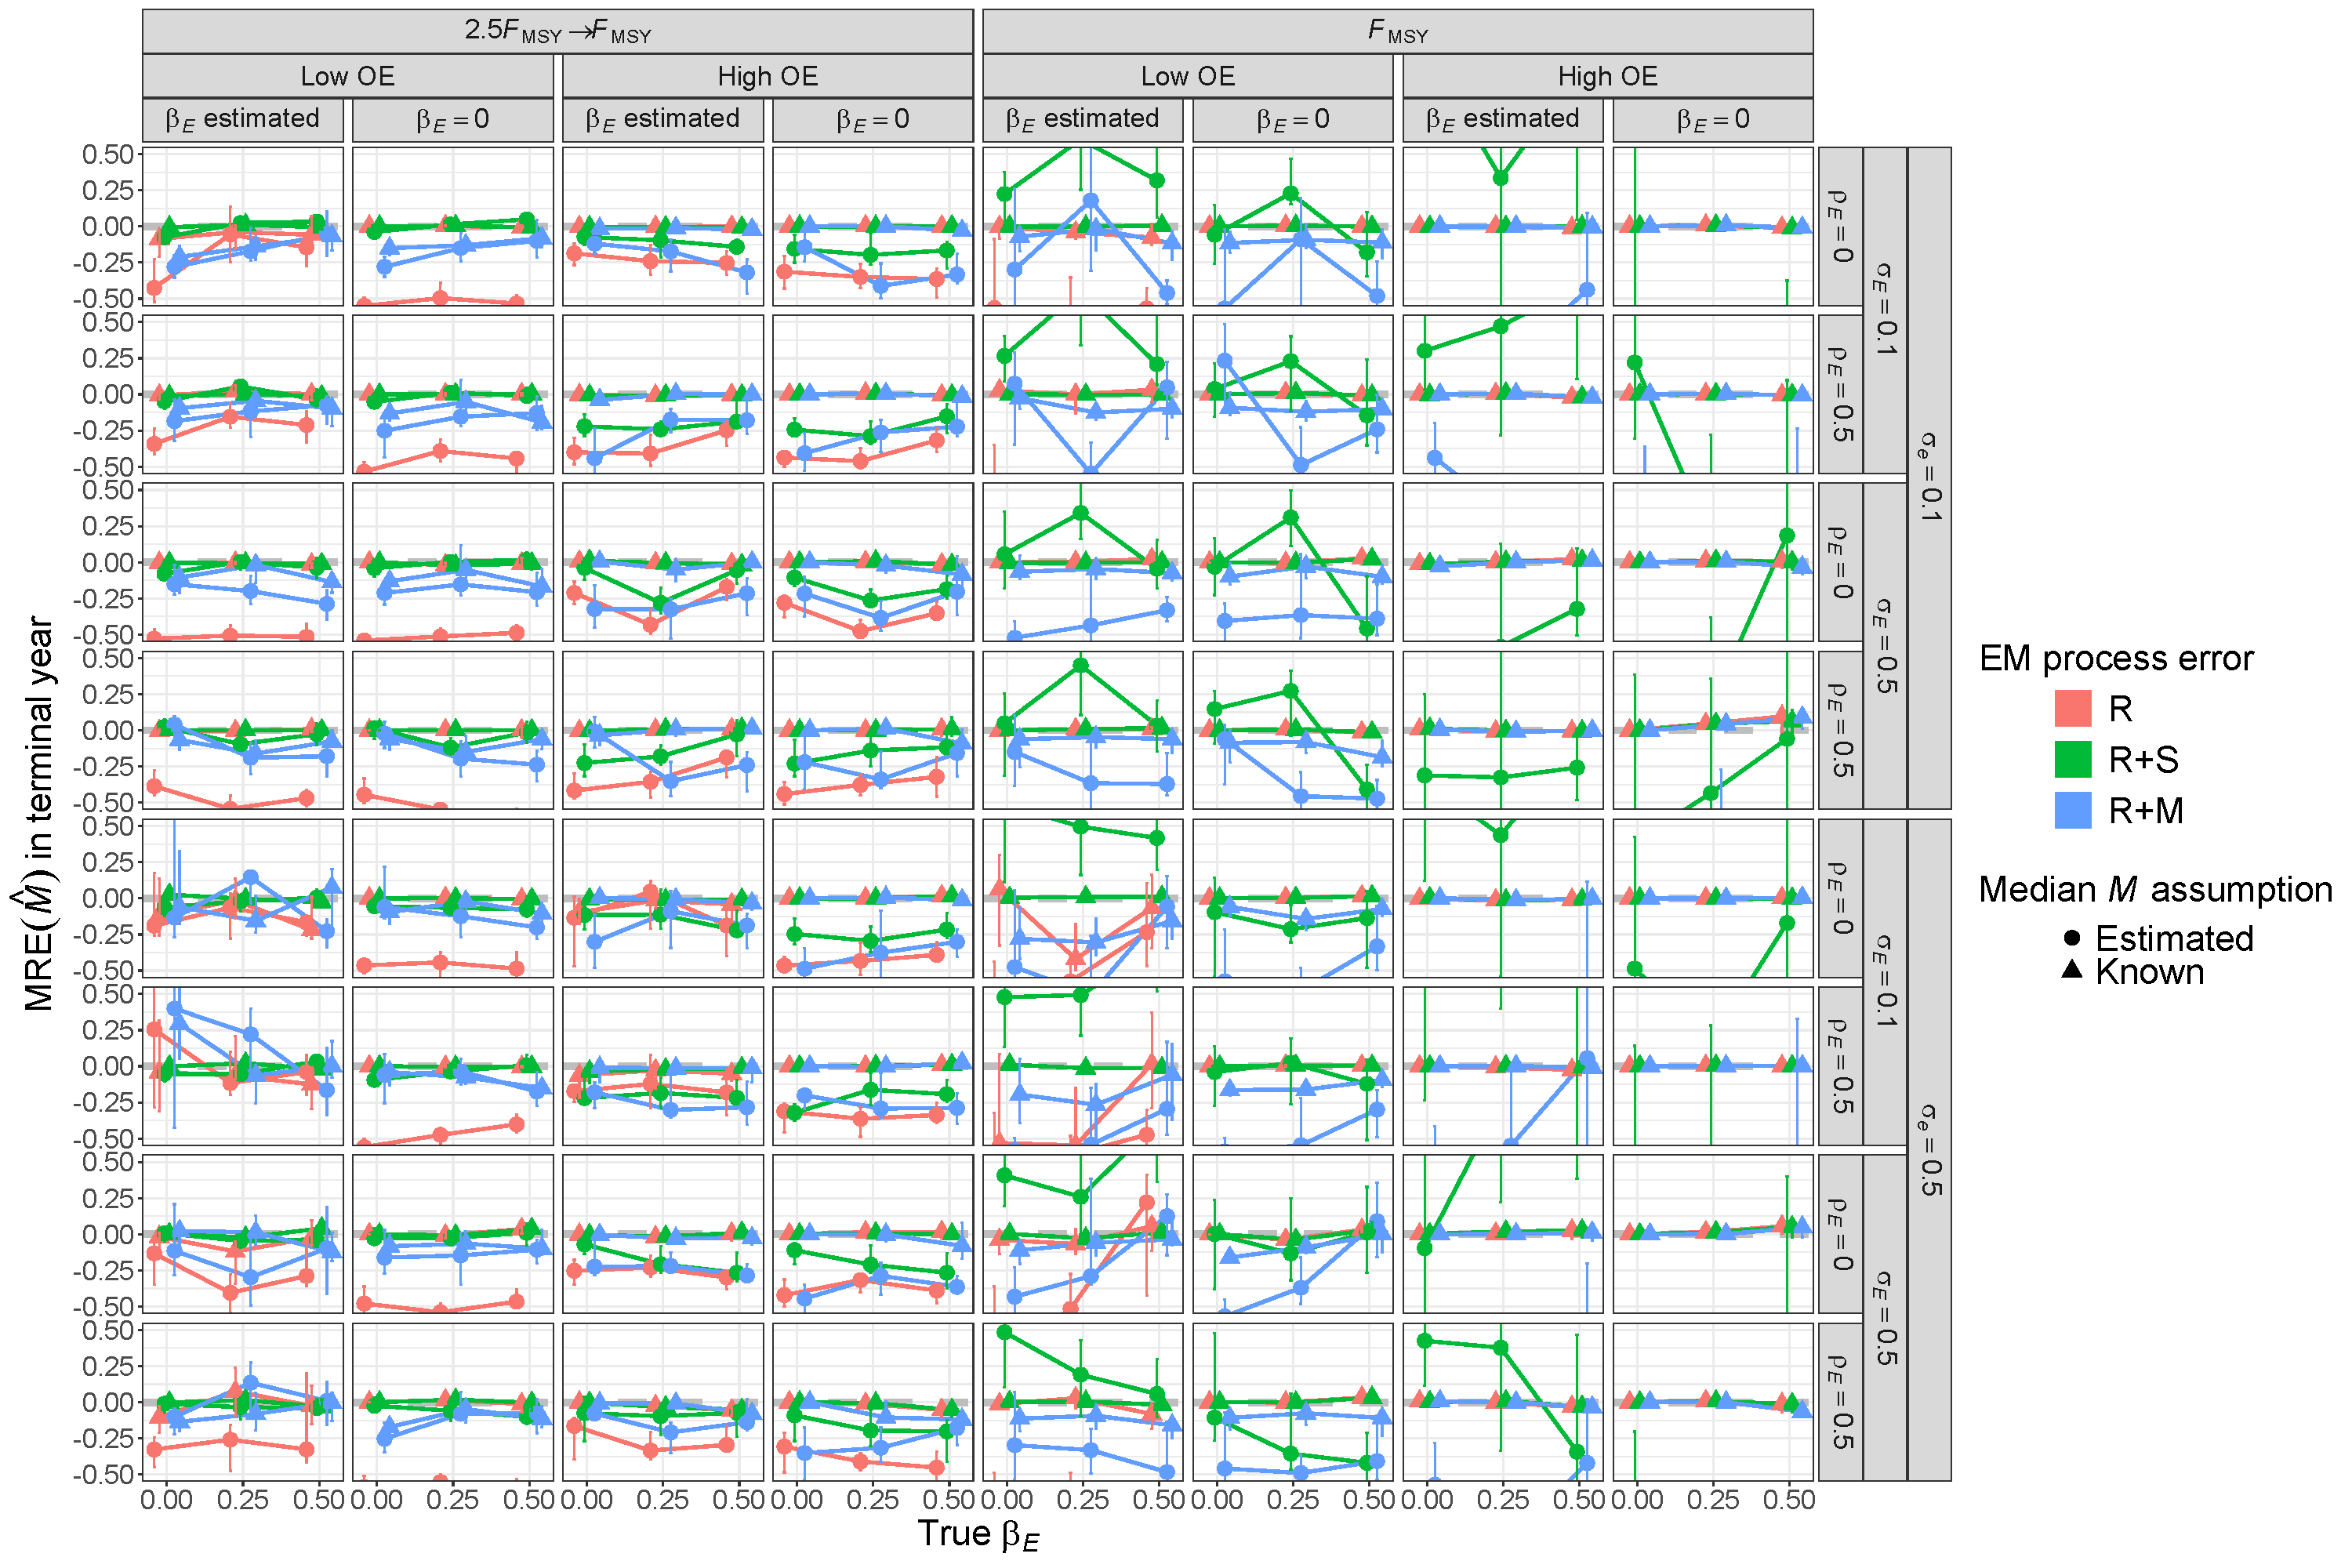
\includegraphics[height = \textheight]{terminal_year_M_bias_RSom}
\end{center}
\caption{For R+S operating models, median relative error (MRE) of estimates of terminal year $M$ for estimating models with alternative process error assumptions, treatment of covariate effect ($\beta_E = 0$ or estimated), and treatment of median $M$ parameter ($\beta_M$ estimated or known).}\label{terminal_M_bias_RSom}
\end{figure}
\end{landscape}

\begin{landscape}
\begin{figure}
\begin{center}
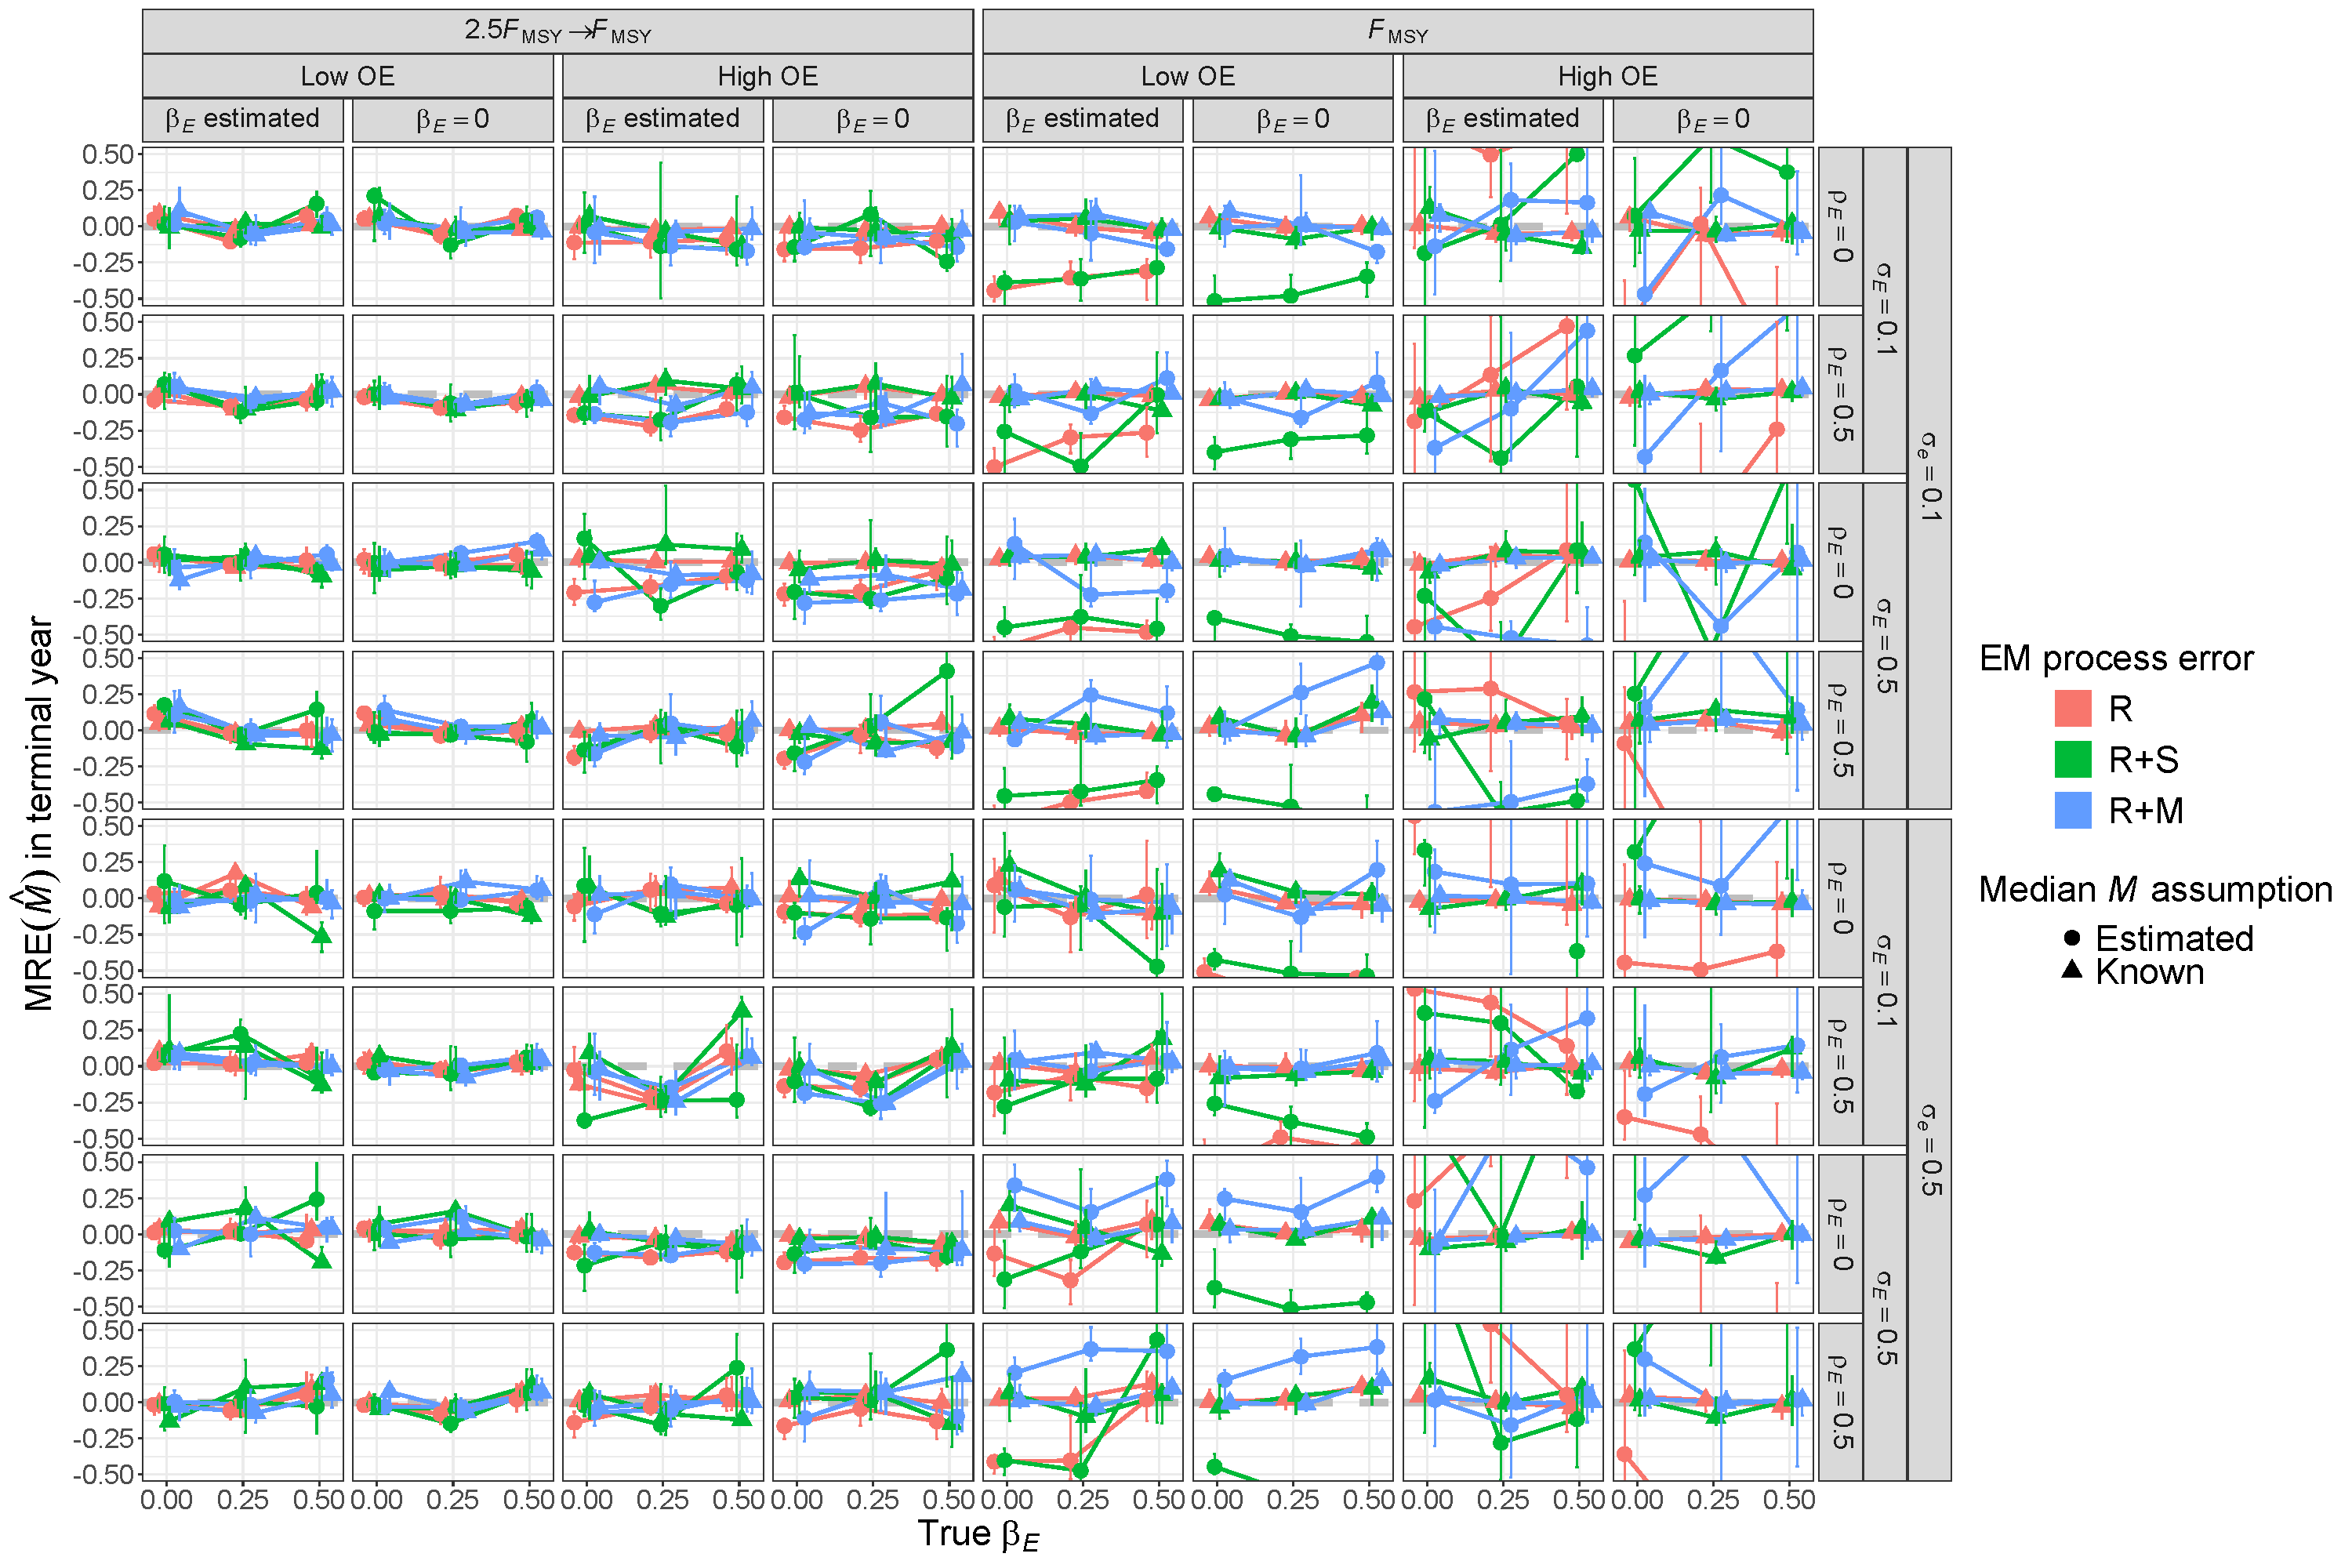
\includegraphics[height = \textheight]{terminal_year_M_bias_RMom}
\end{center}
\caption{For R+M operating models, median relative error (MRE) of estimates of terminal year $M$ for estimating models with alternative process error assumptions, treatment of covariate effect ($\beta_E = 0$ or estimated), and treatment of median $M$ parameter ($\beta_M$ estimated or known).}\label{terminal_M_bias_RMom}
\end{figure}
\end{landscape}

\begin{landscape}
\begin{figure}
\begin{center}
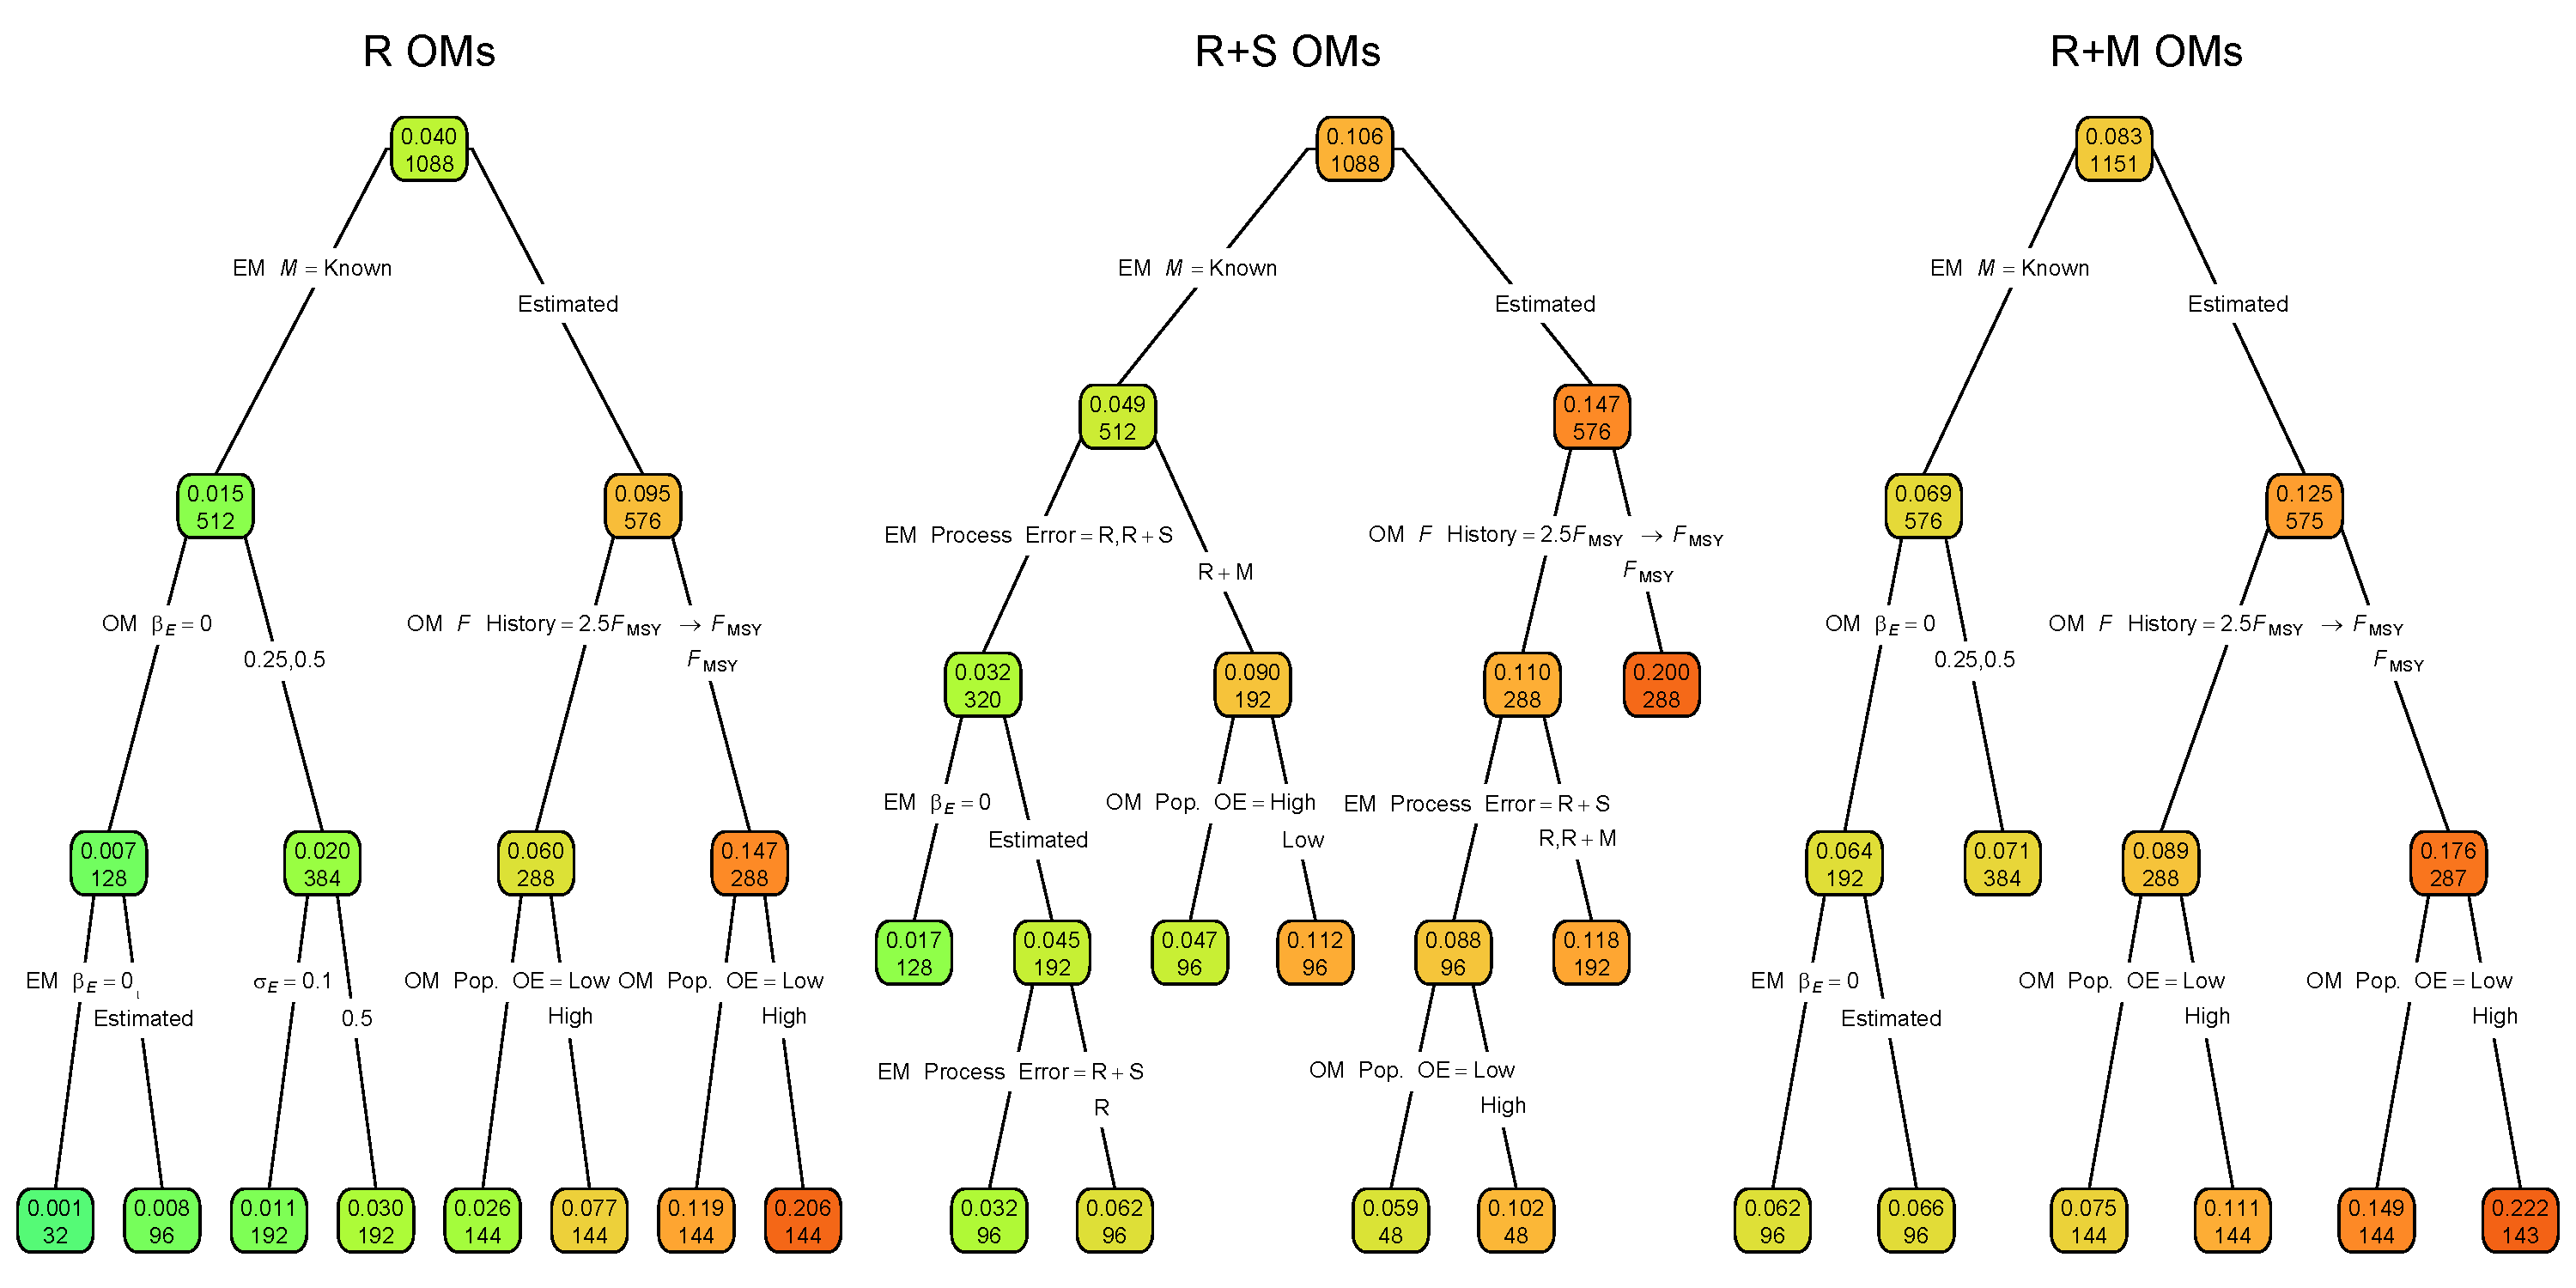
\includegraphics[width = 1.4\textwidth]{term_M_rmse_regtree_plots}
\end{center}
\caption{Regression trees for the log-transformed RMSE of terminal year $M$. Each node shows the median RMSE (top) and number of observations (bottom) for the corresponding subset. Lower or higher median RMSE are indicated by more green or red polygons, respectively. See Figure \ref{conv_class} caption and Table \ref{factor_table} for further details.}\label{term_M_rmse_regtree}
\end{figure}
\end{landscape}

\begin{landscape}
\begin{figure}
\begin{center}
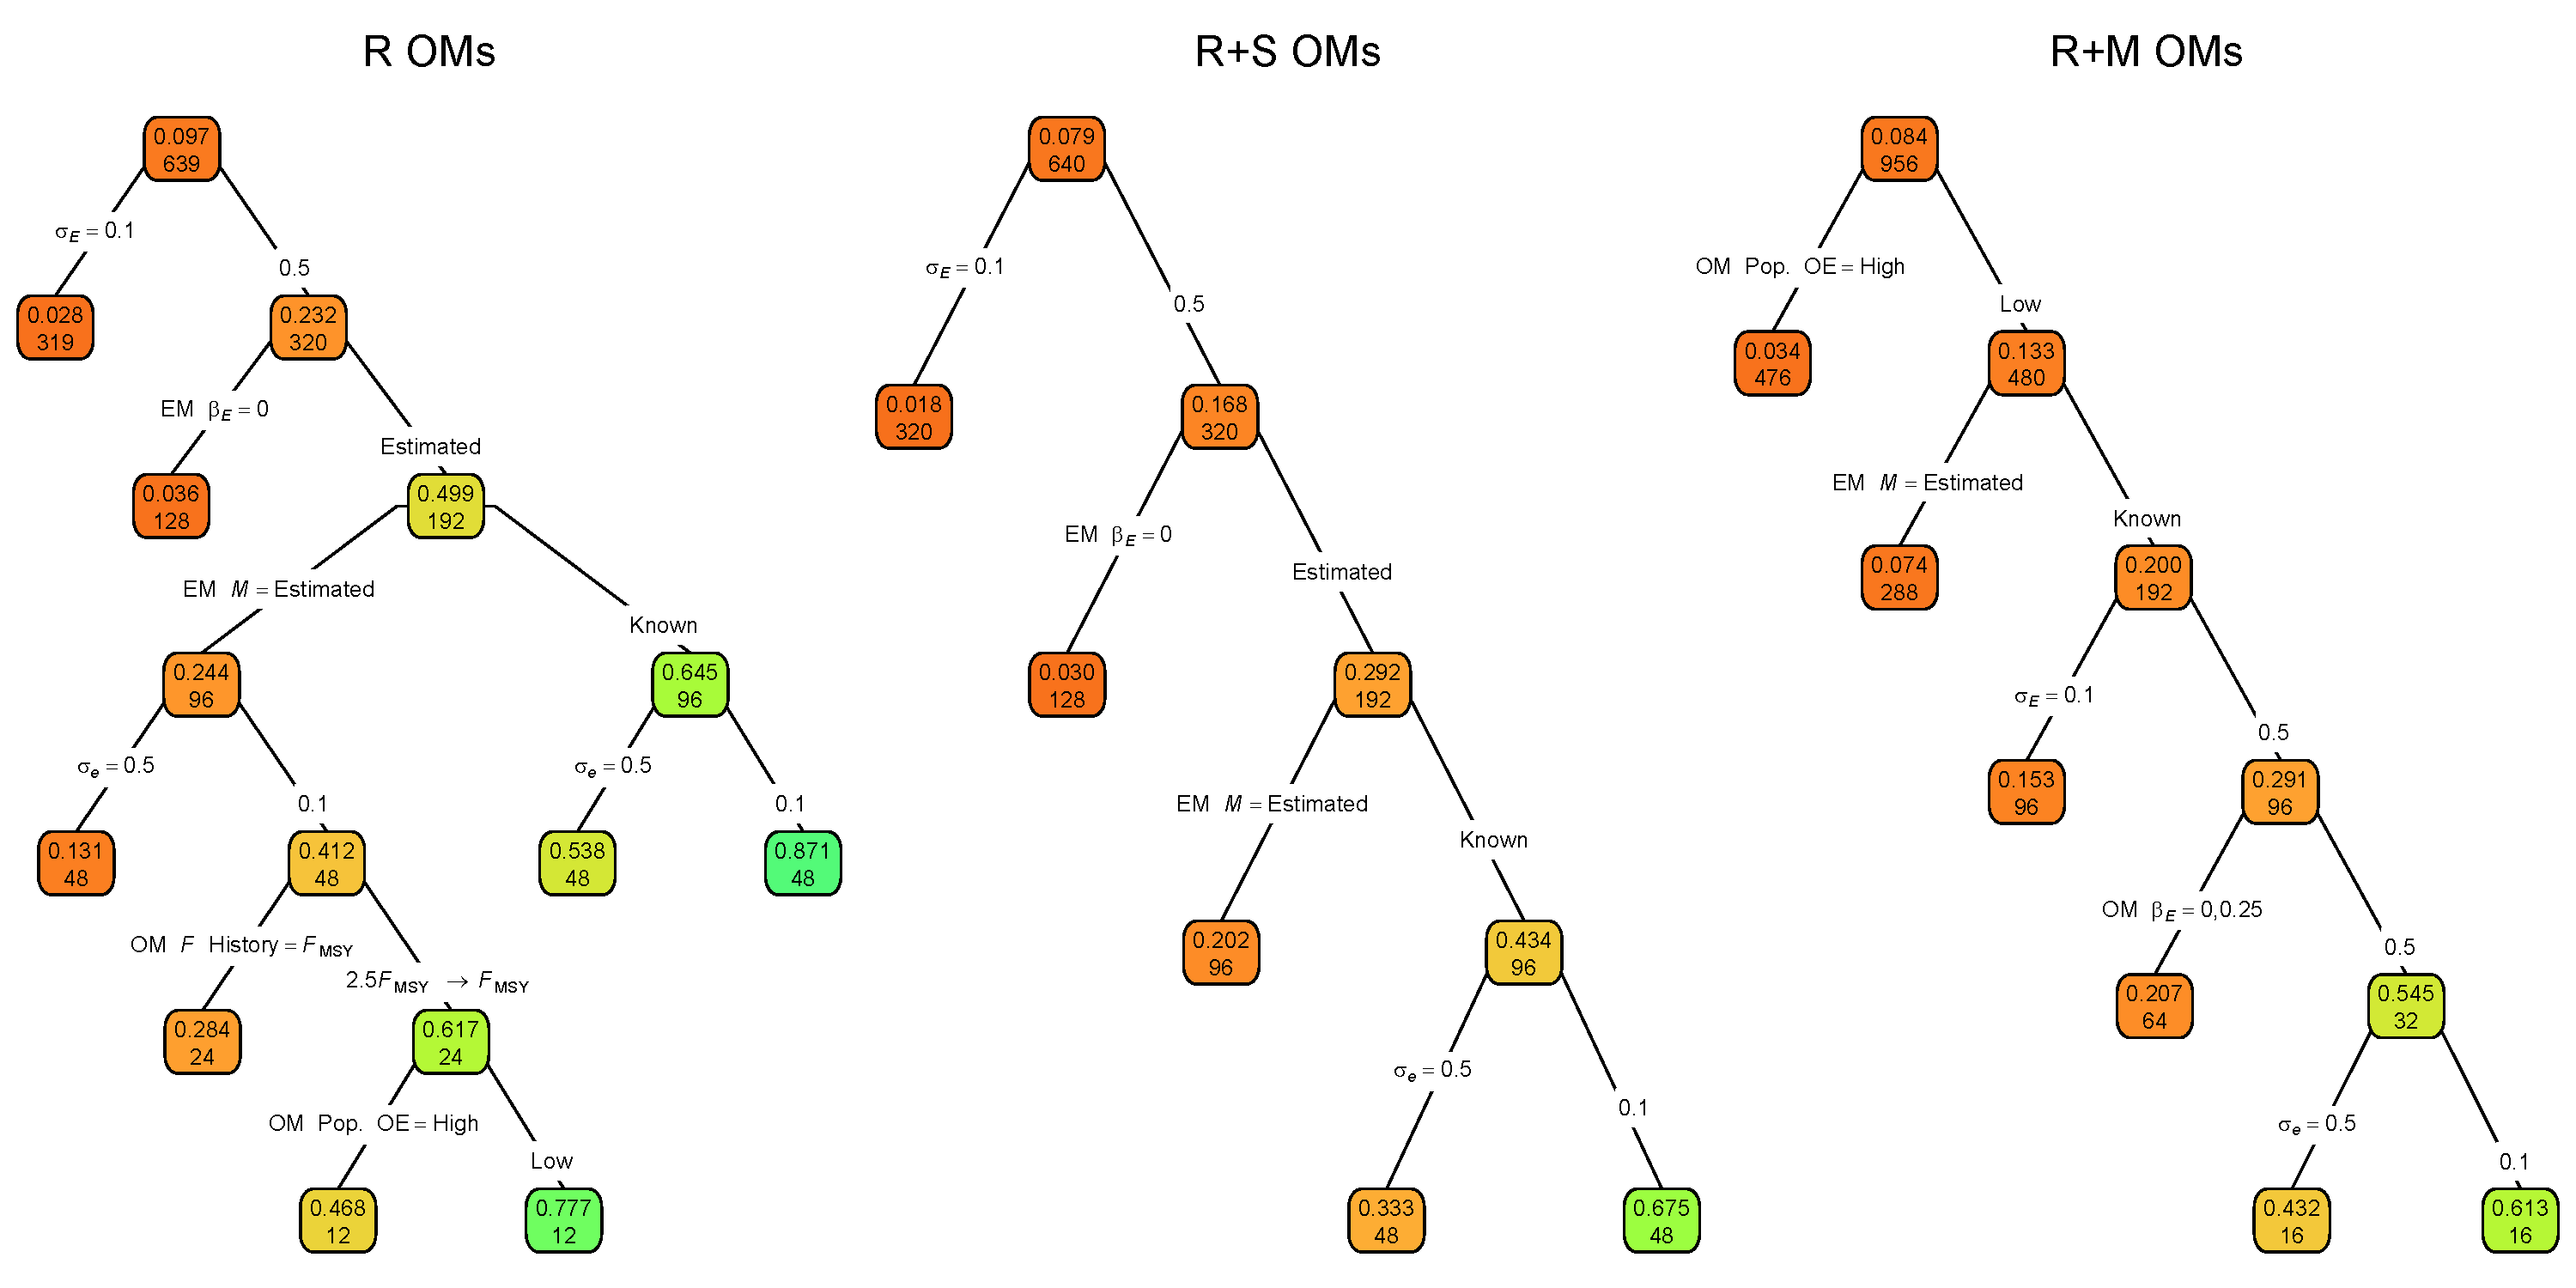
\includegraphics[width = 1.4\textwidth]{term_M_corr_regtree_plots}
\end{center}
\caption{Regression trees for the correlation of terminal year $M$ estimates and true values. Each node shows the median correlation for the corresponding subset. Lower or higher median correlations are indicated by more red or green polygons, respectively. See Figure \ref{conv_class} caption and Table \ref{factor_table} for further details.}\label{term_M_corr_regtree}
\end{figure}
\end{landscape}

\begin{landscape}
\begin{figure}
\begin{center}
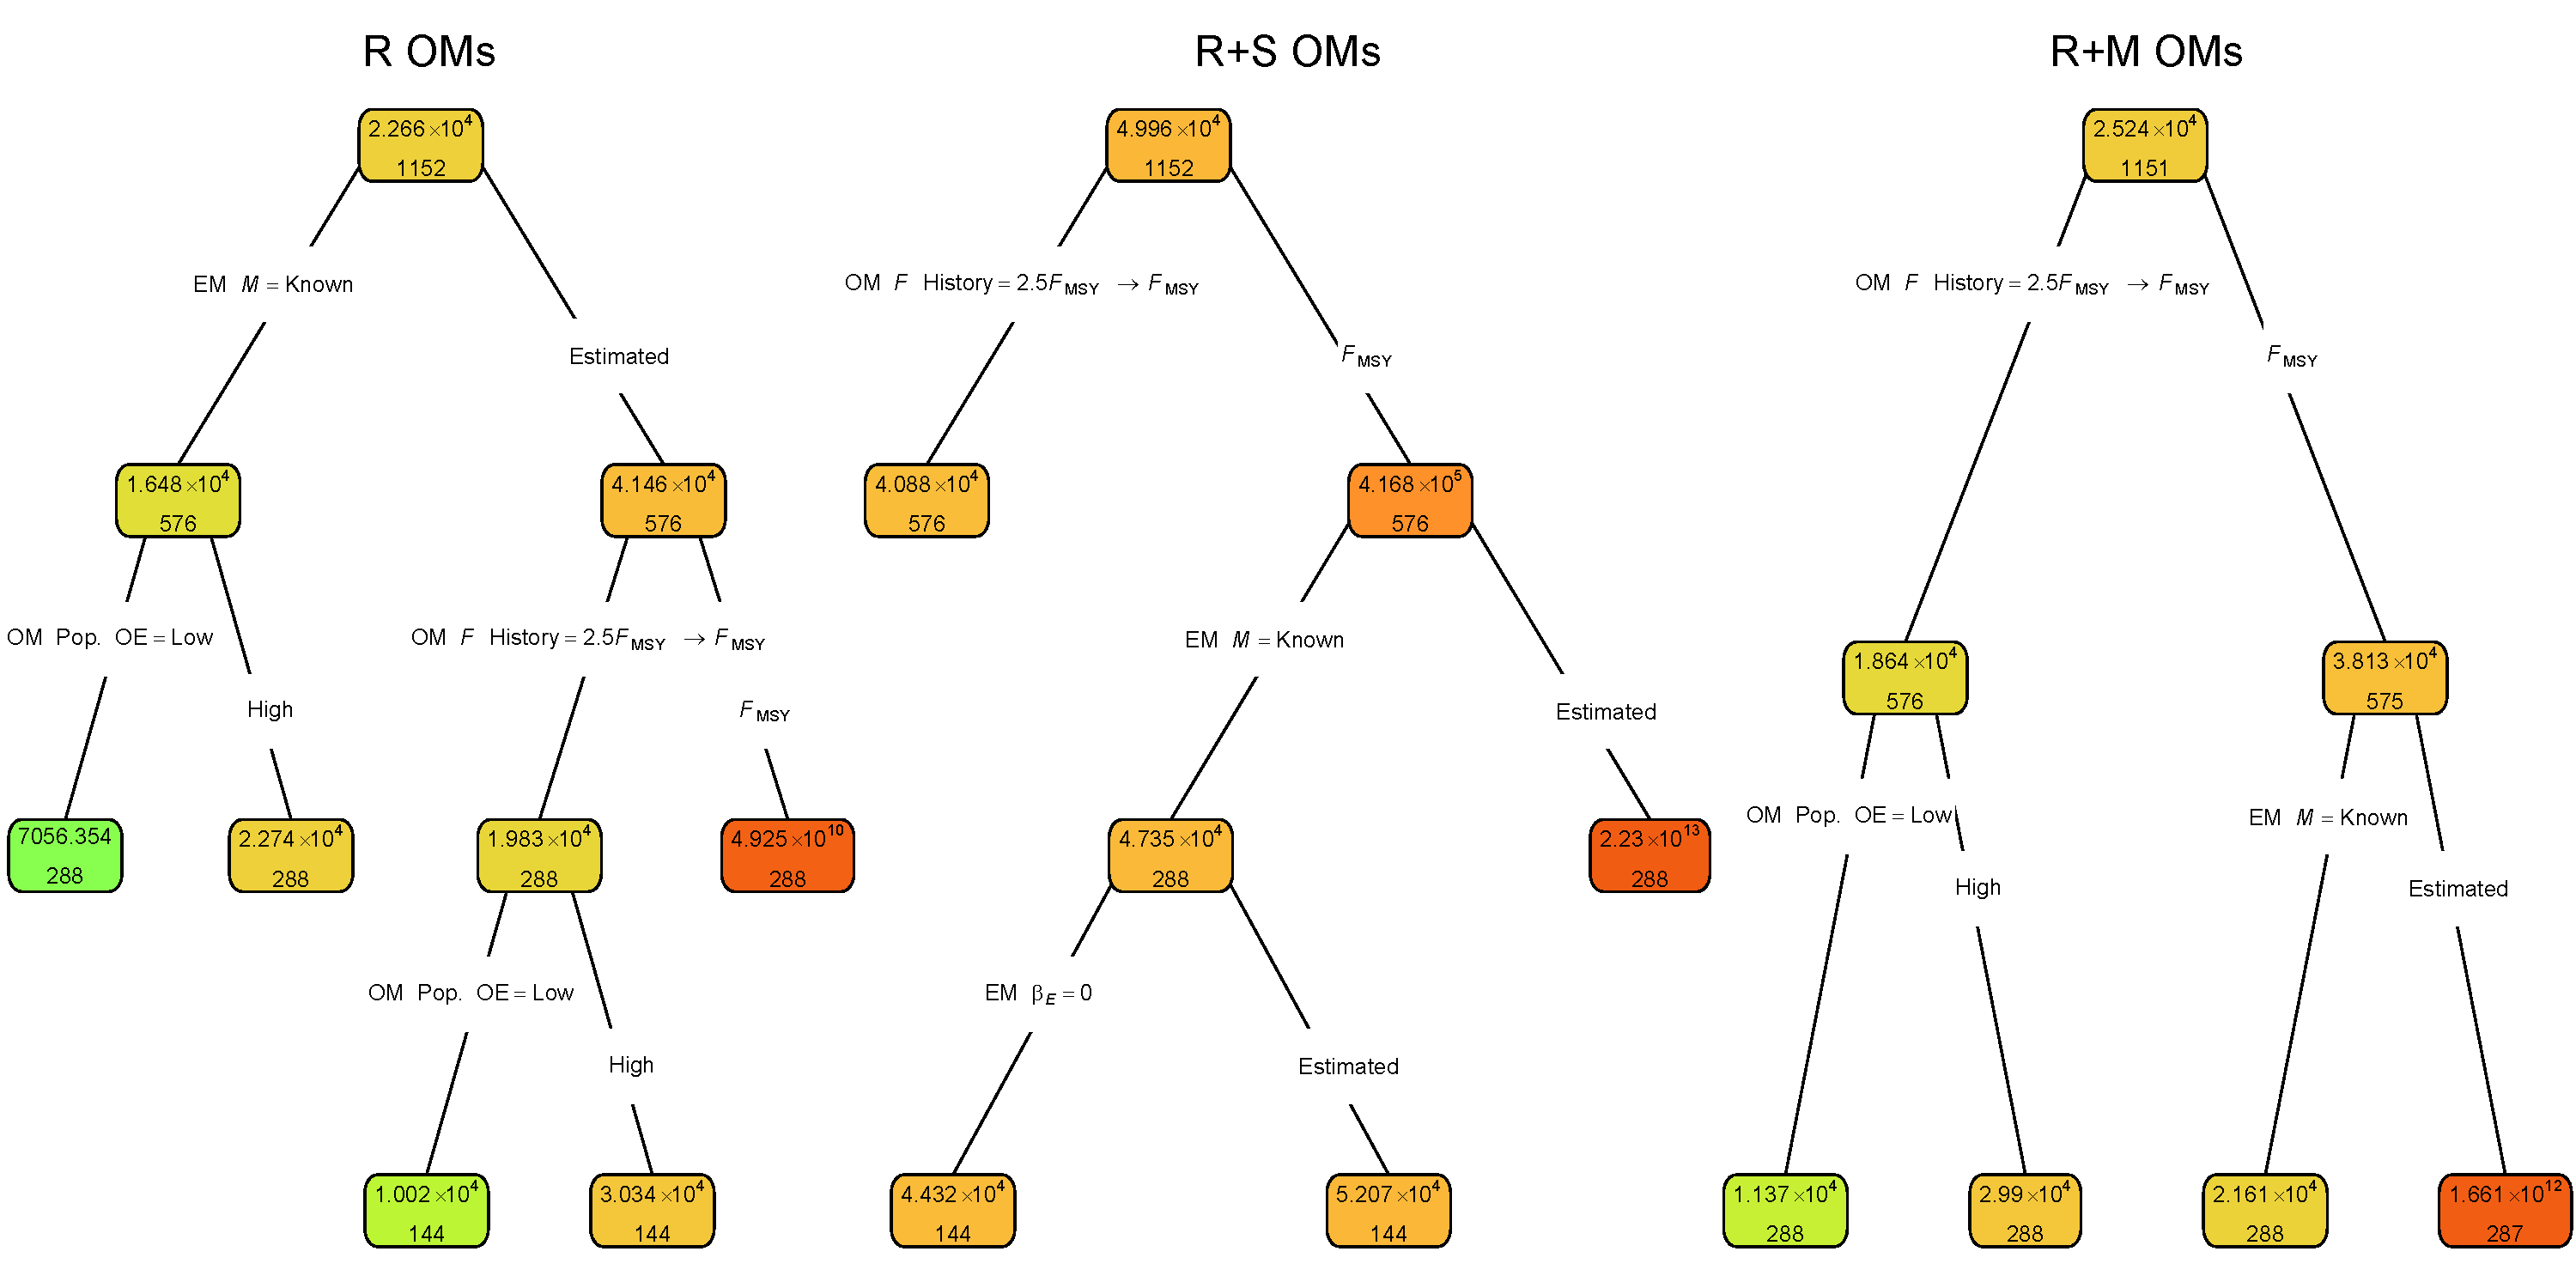
\includegraphics[width = 1.4\textwidth]{term_SSB_rmse_regtree_plots}
\end{center}
\caption{Regression trees for the log-transformed RMSE of terminal year SSB. Each node shows the median RMSE (top) and number of observations (bottom) for the corresponding subset. Lower or higher median RMSE are indicated by more red or green polygons, respectively.}\label{term_SSB_rmse_regtree}
\end{figure}
\end{landscape}

\begin{landscape}
\begin{figure}
\begin{center}
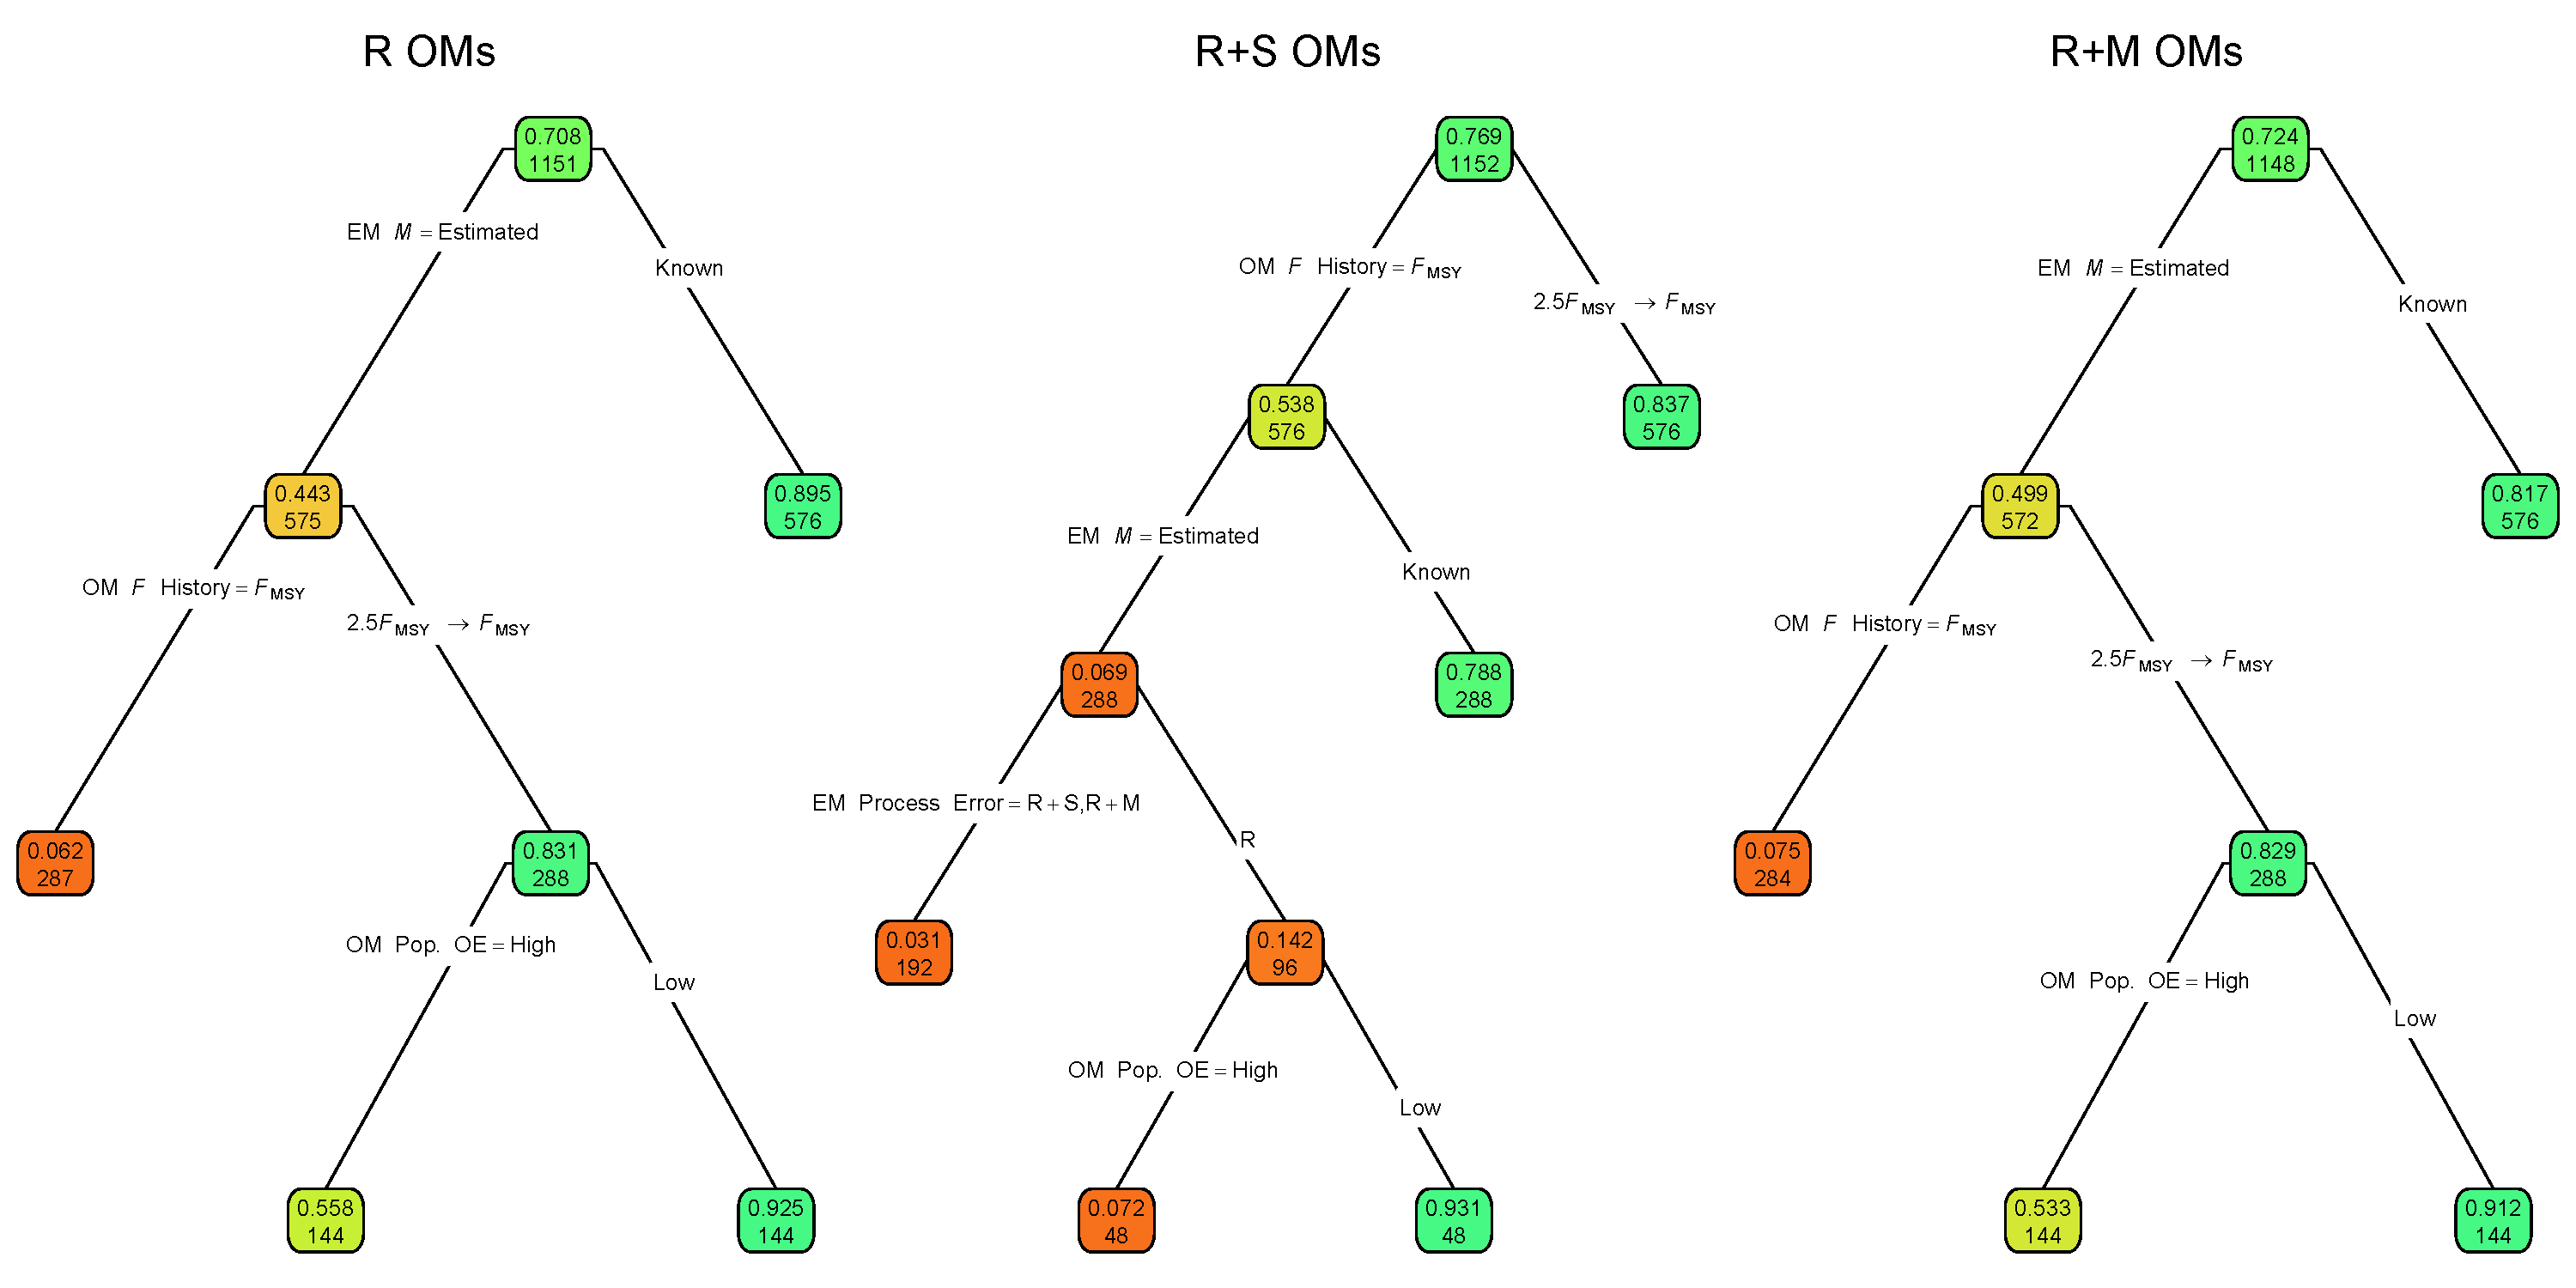
\includegraphics[width = 1.4\textwidth]{term_ssb_corr_regtree_plots}
\end{center}
\caption{Regression trees for the correlation of terminal year SSB estimates and true values. Each node shows the median correlation for the corresponding subset. Lower or higher median correlations are indicated by more red or green polygons, respectively. See Figure \ref{conv_class} caption and Table \ref{factor_table} for further details.}\label{term_ssb_corr_regtree}
\end{figure}
\end{landscape}
\pagebreak

\begin{landscape}
\begin{figure}
\begin{center}
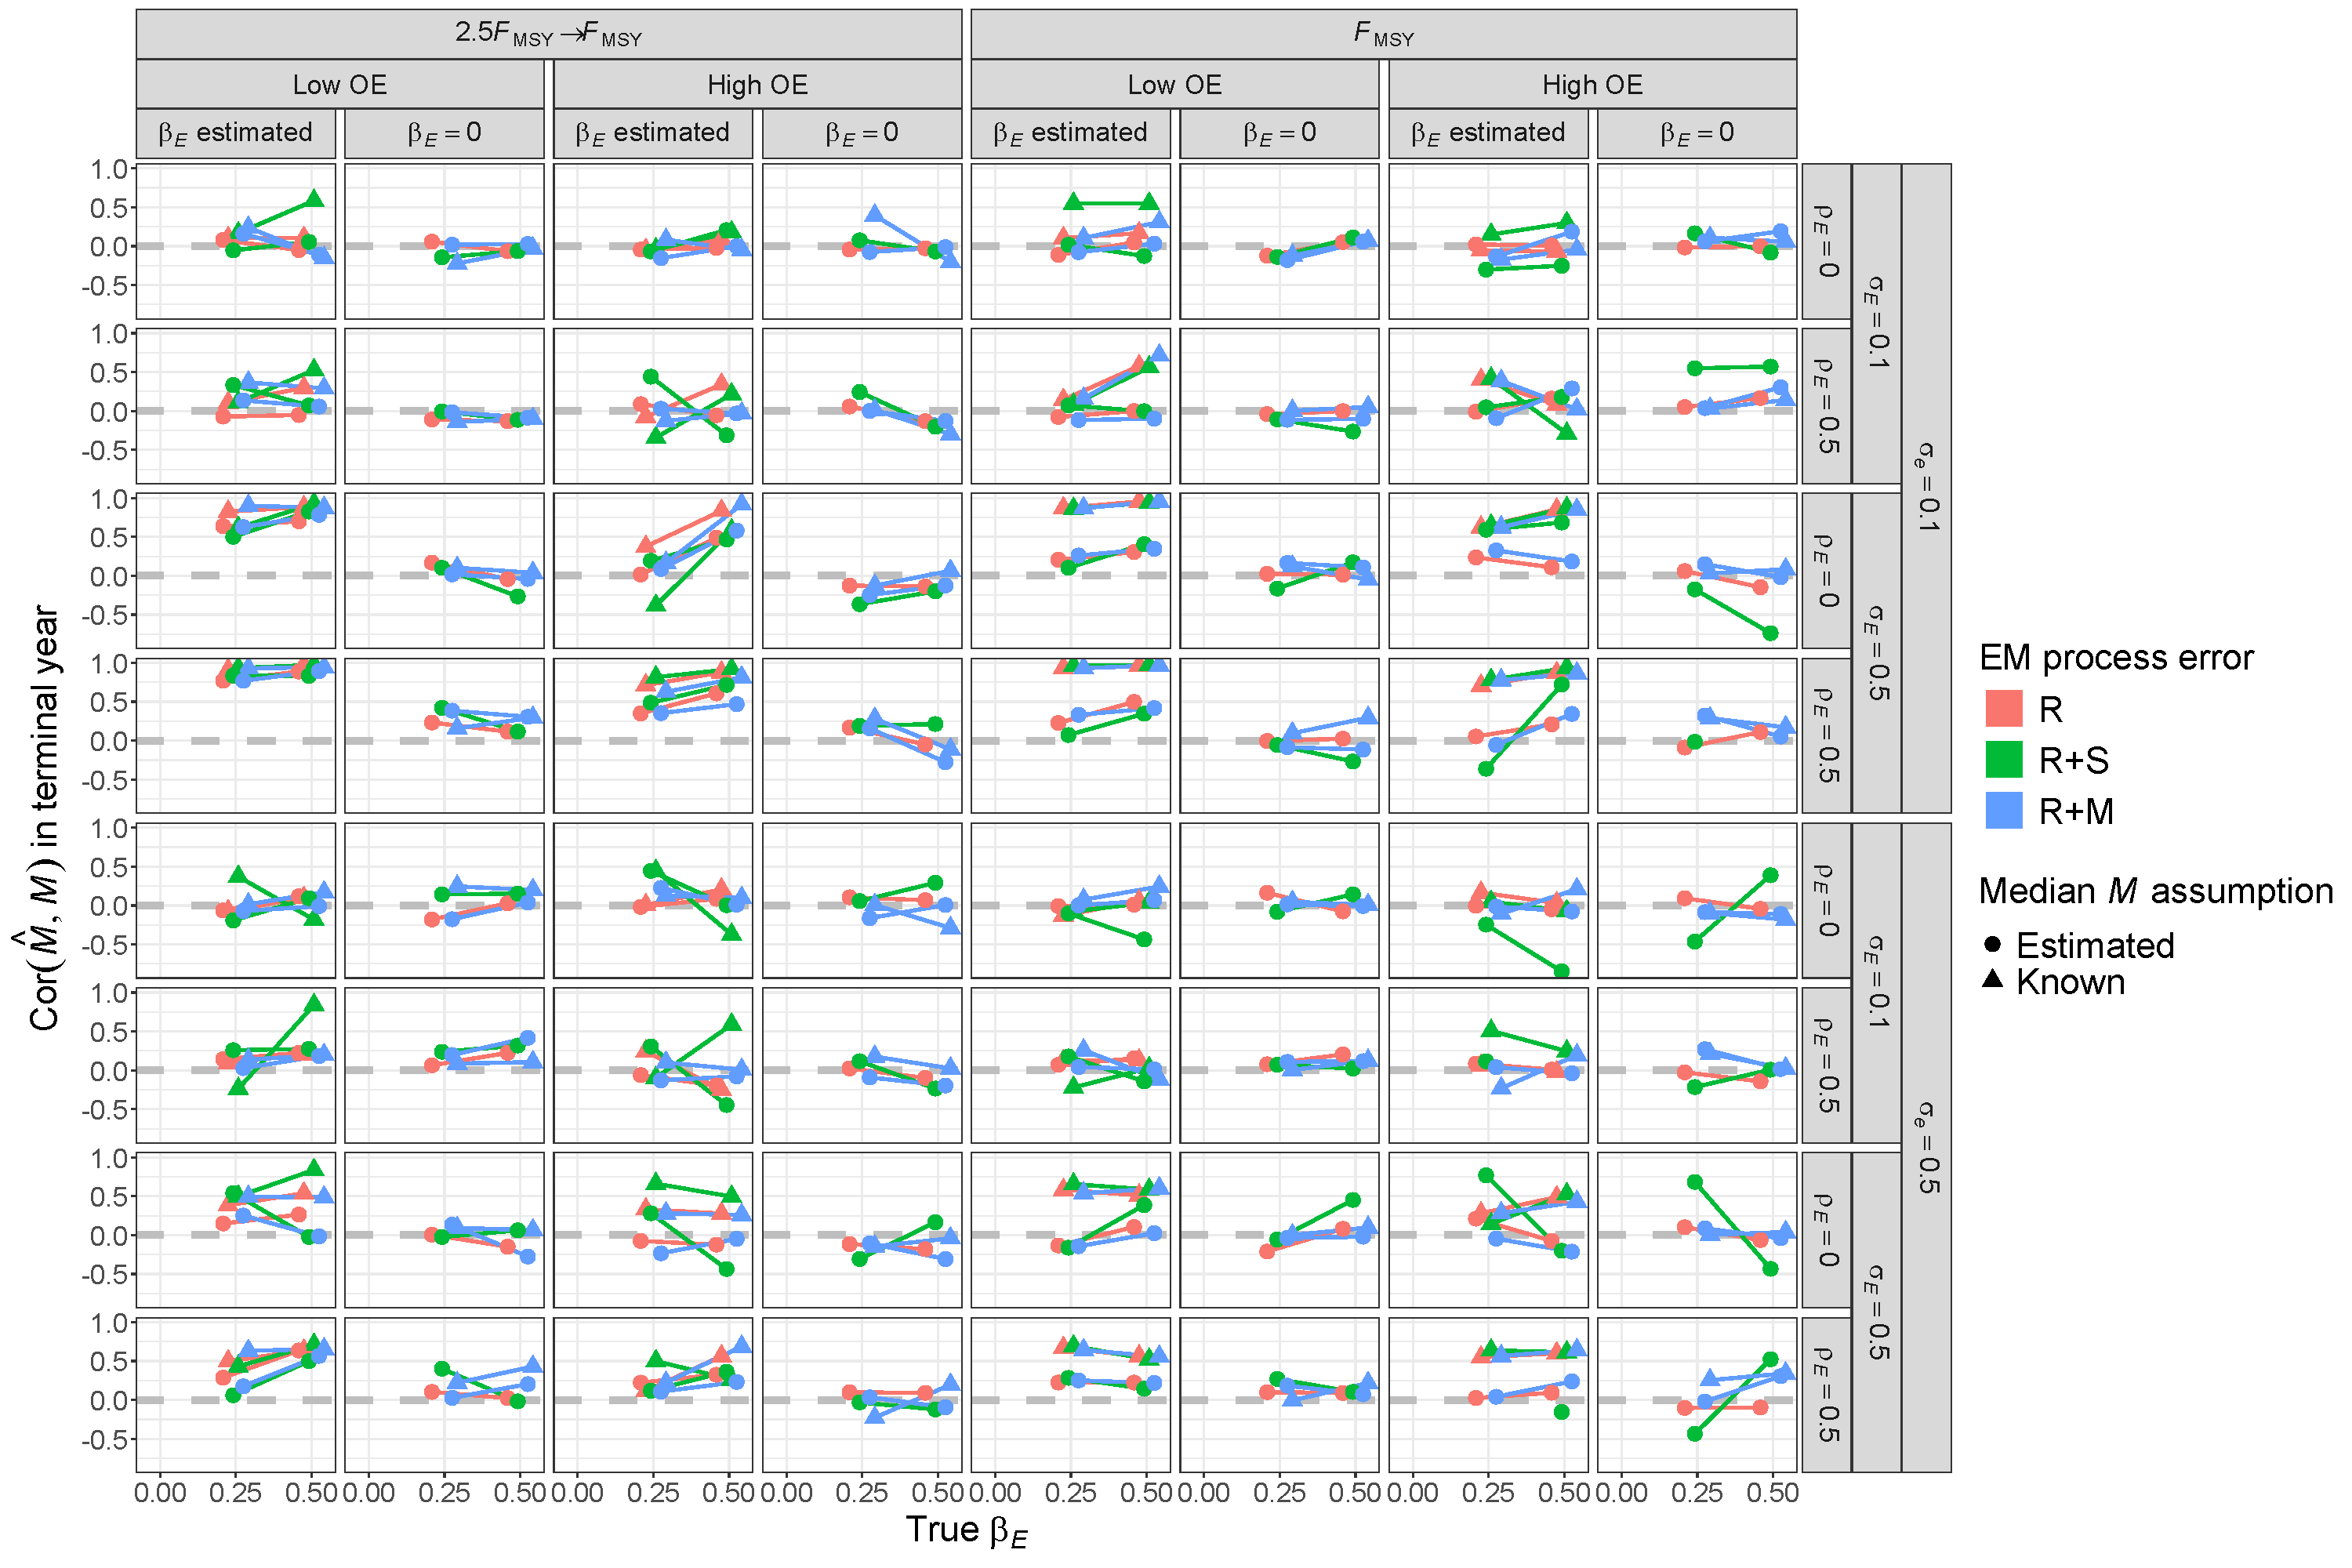
\includegraphics[height = \textheight]{terminal_year_M_corr_Rom}
\end{center}
\caption{For R operating models, correlation of estimates and true values of terminal year $M$ for estimating models with alternative process error assumptions, treatment of covariate effect ($\beta_E = 0$ or estimated), and treatment of median $M$ parameter ($\beta_M$ estimated or known).}\label{terminal_M_corr_Rom}
\end{figure}
\end{landscape}

\begin{landscape}
\begin{figure}
\begin{center}
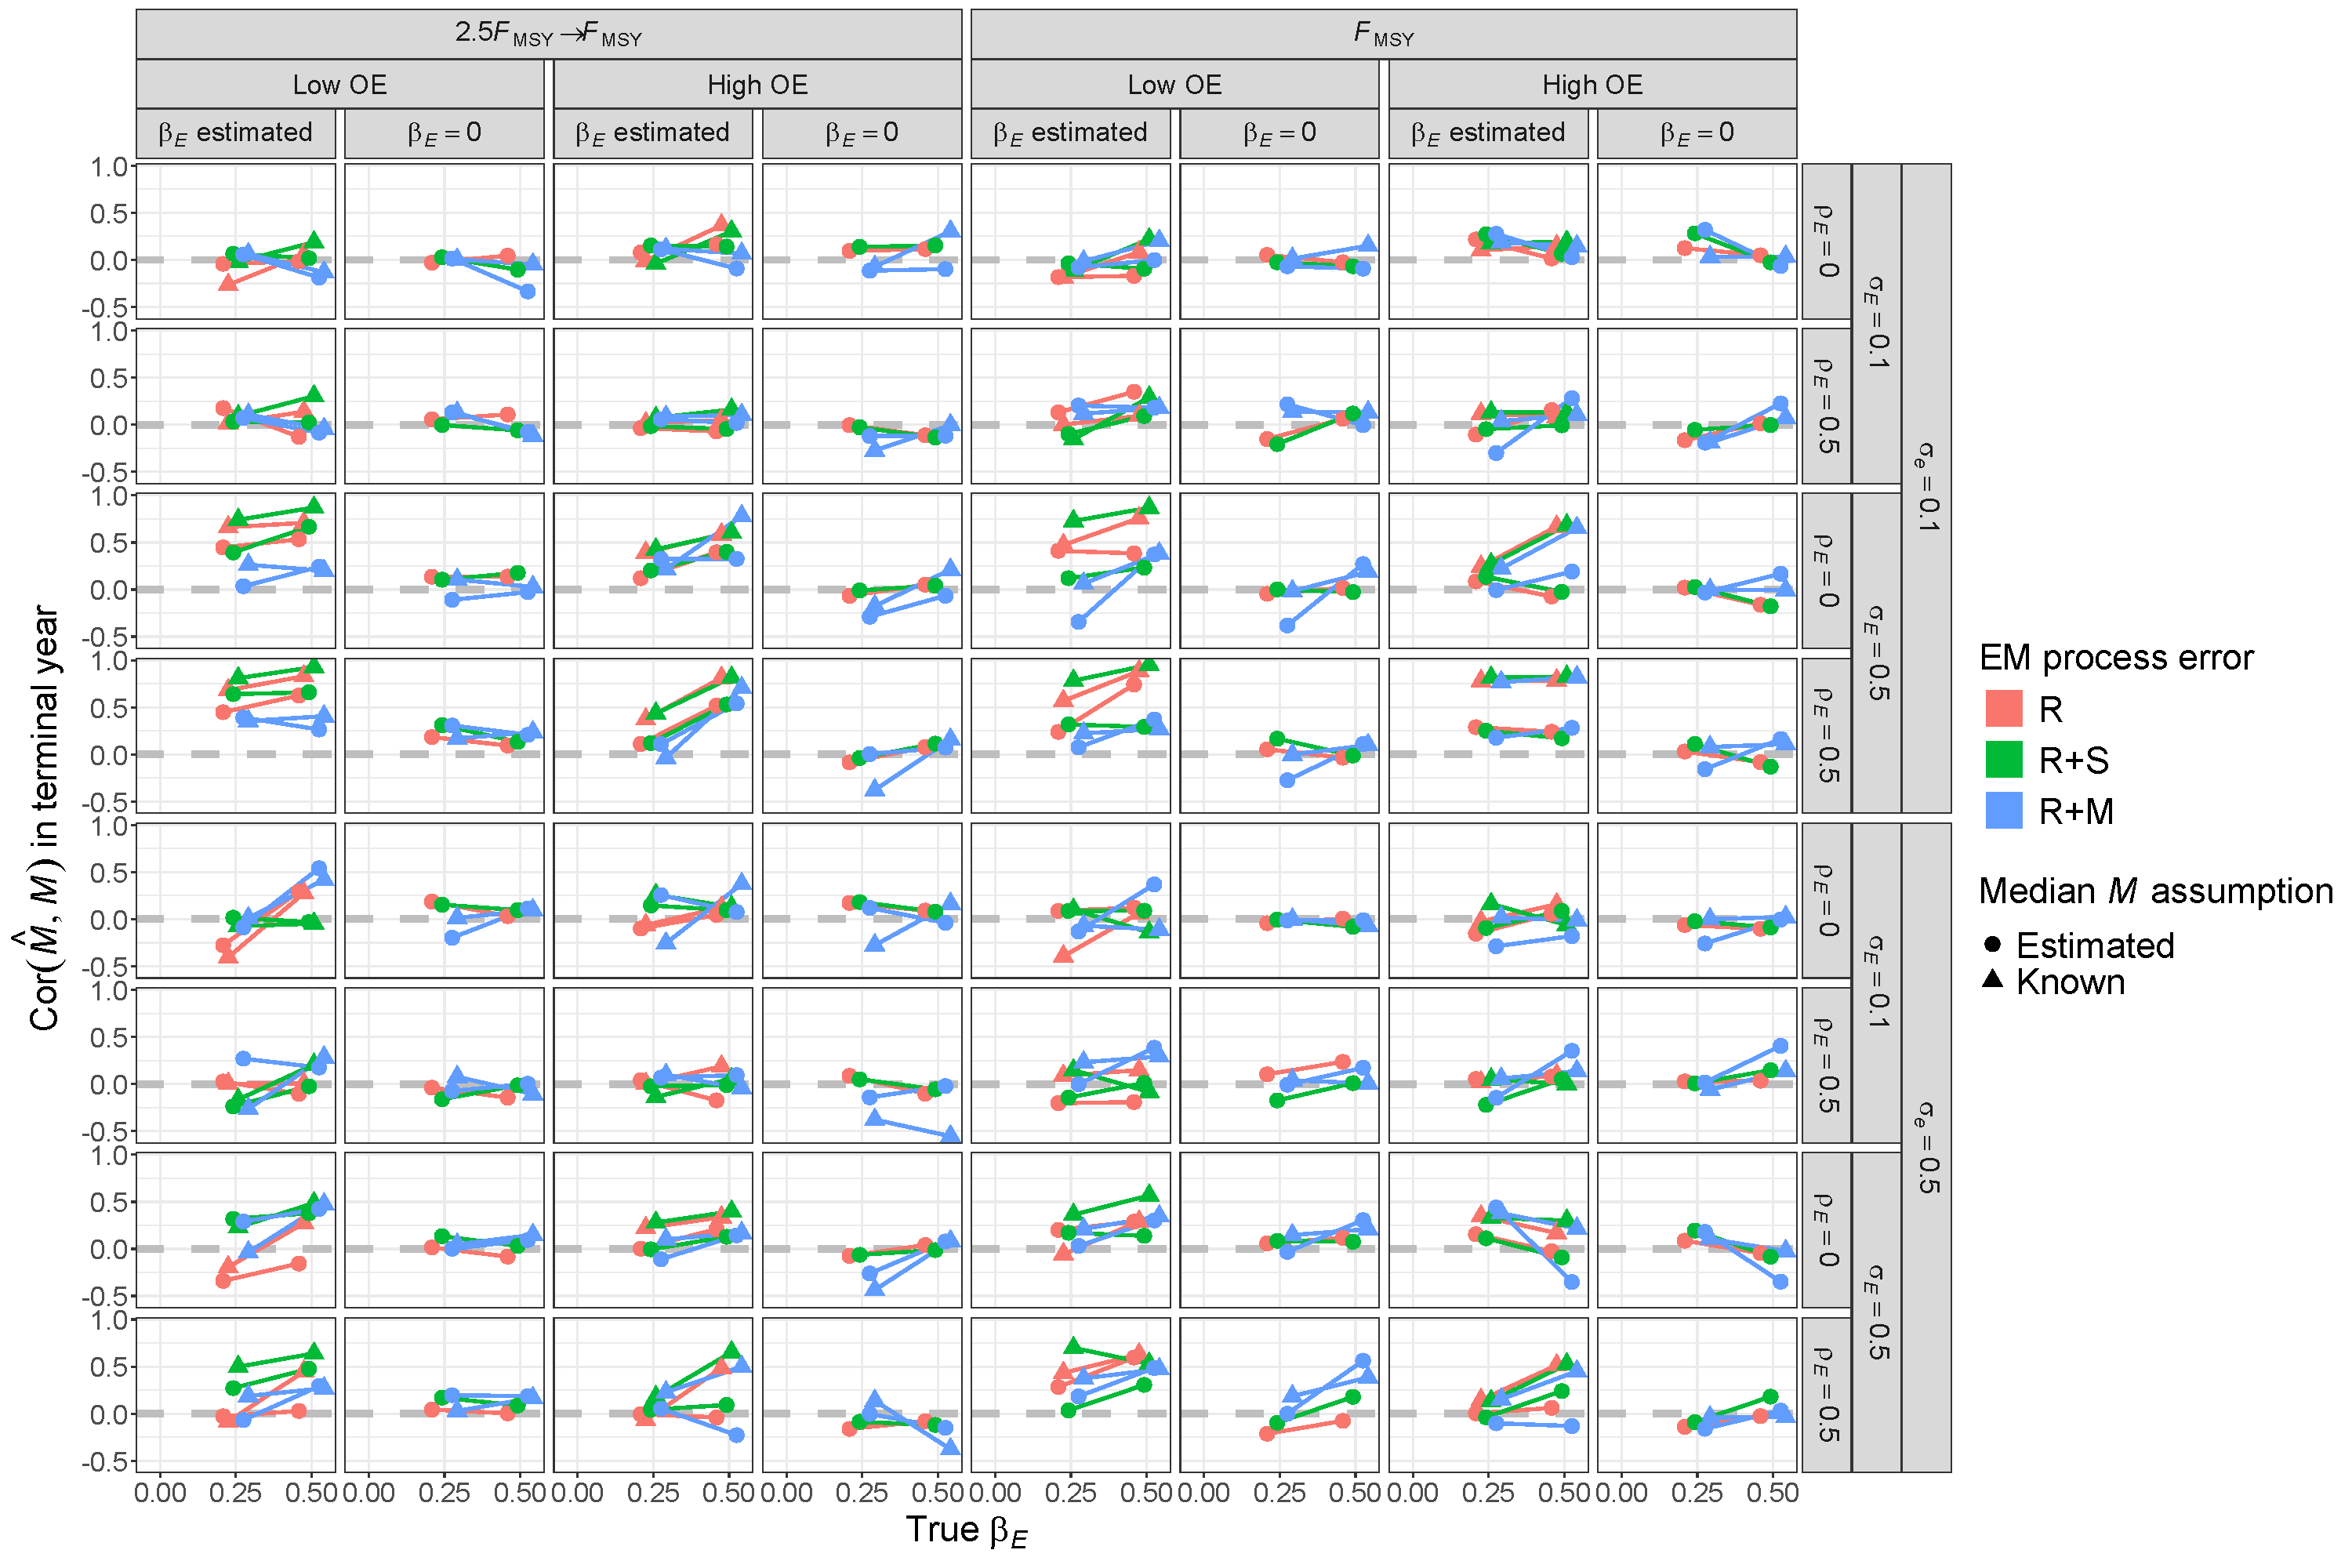
\includegraphics[height = \textheight]{terminal_year_M_corr_RSom}
\end{center}
\caption{For R+S operating models, correlation of estimates and true values of terminal year $M$ for estimating models with alternative process error assumptions, treatment of covariate effect ($\beta_E = 0$ or estimated), and treatment of median $M$ parameter ($\beta_M$ estimated or known).}\label{terminal_M_corr_RSom}
\end{figure}
\end{landscape}

\begin{landscape}
\begin{figure}
\begin{center}
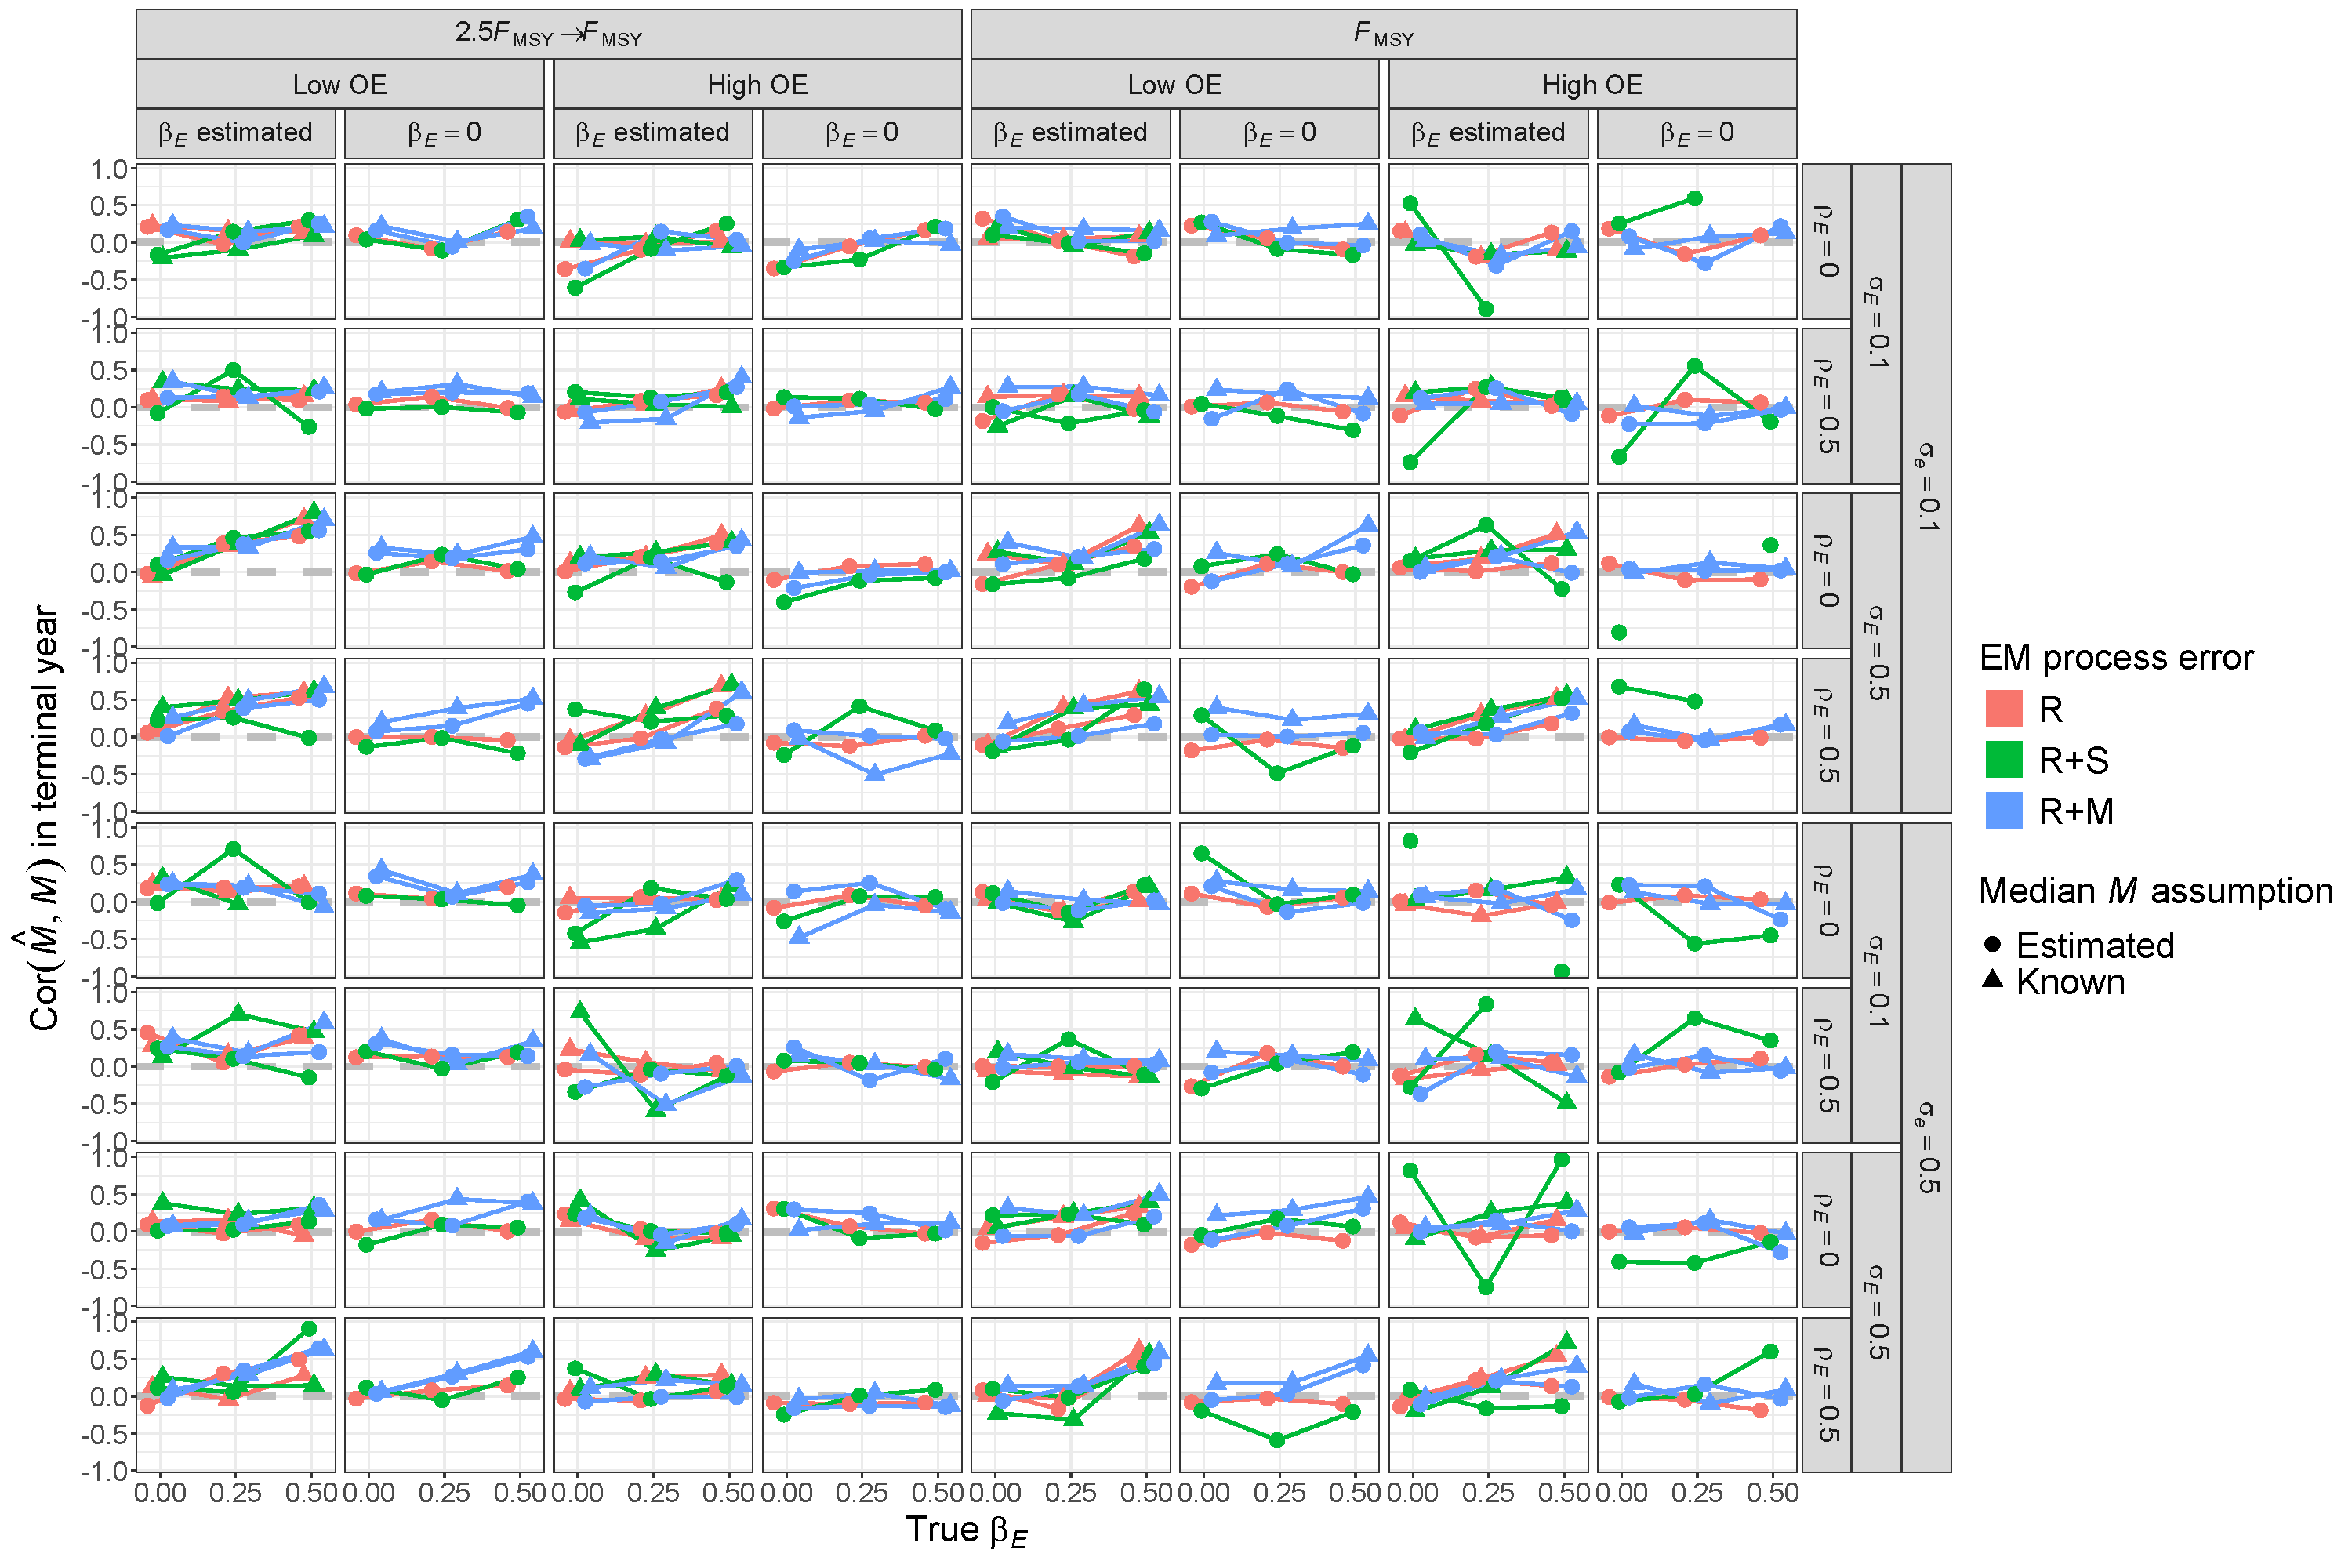
\includegraphics[height = \textheight]{terminal_year_M_corr_RMom}
\end{center}
\caption{For R+M operating models, correlation of estimates and true vales of terminal year $M$ for estimating models with alternative process error assumptions, treatment of covariate effect ($\beta_E = 0$ or estimated), and treatment of median $M$ parameter ($\beta_M$ estimated or known).}\label{terminal_M_corr_RMom}
\end{figure}
\end{landscape}

\begin{landscape}
\begin{figure}
\begin{center}
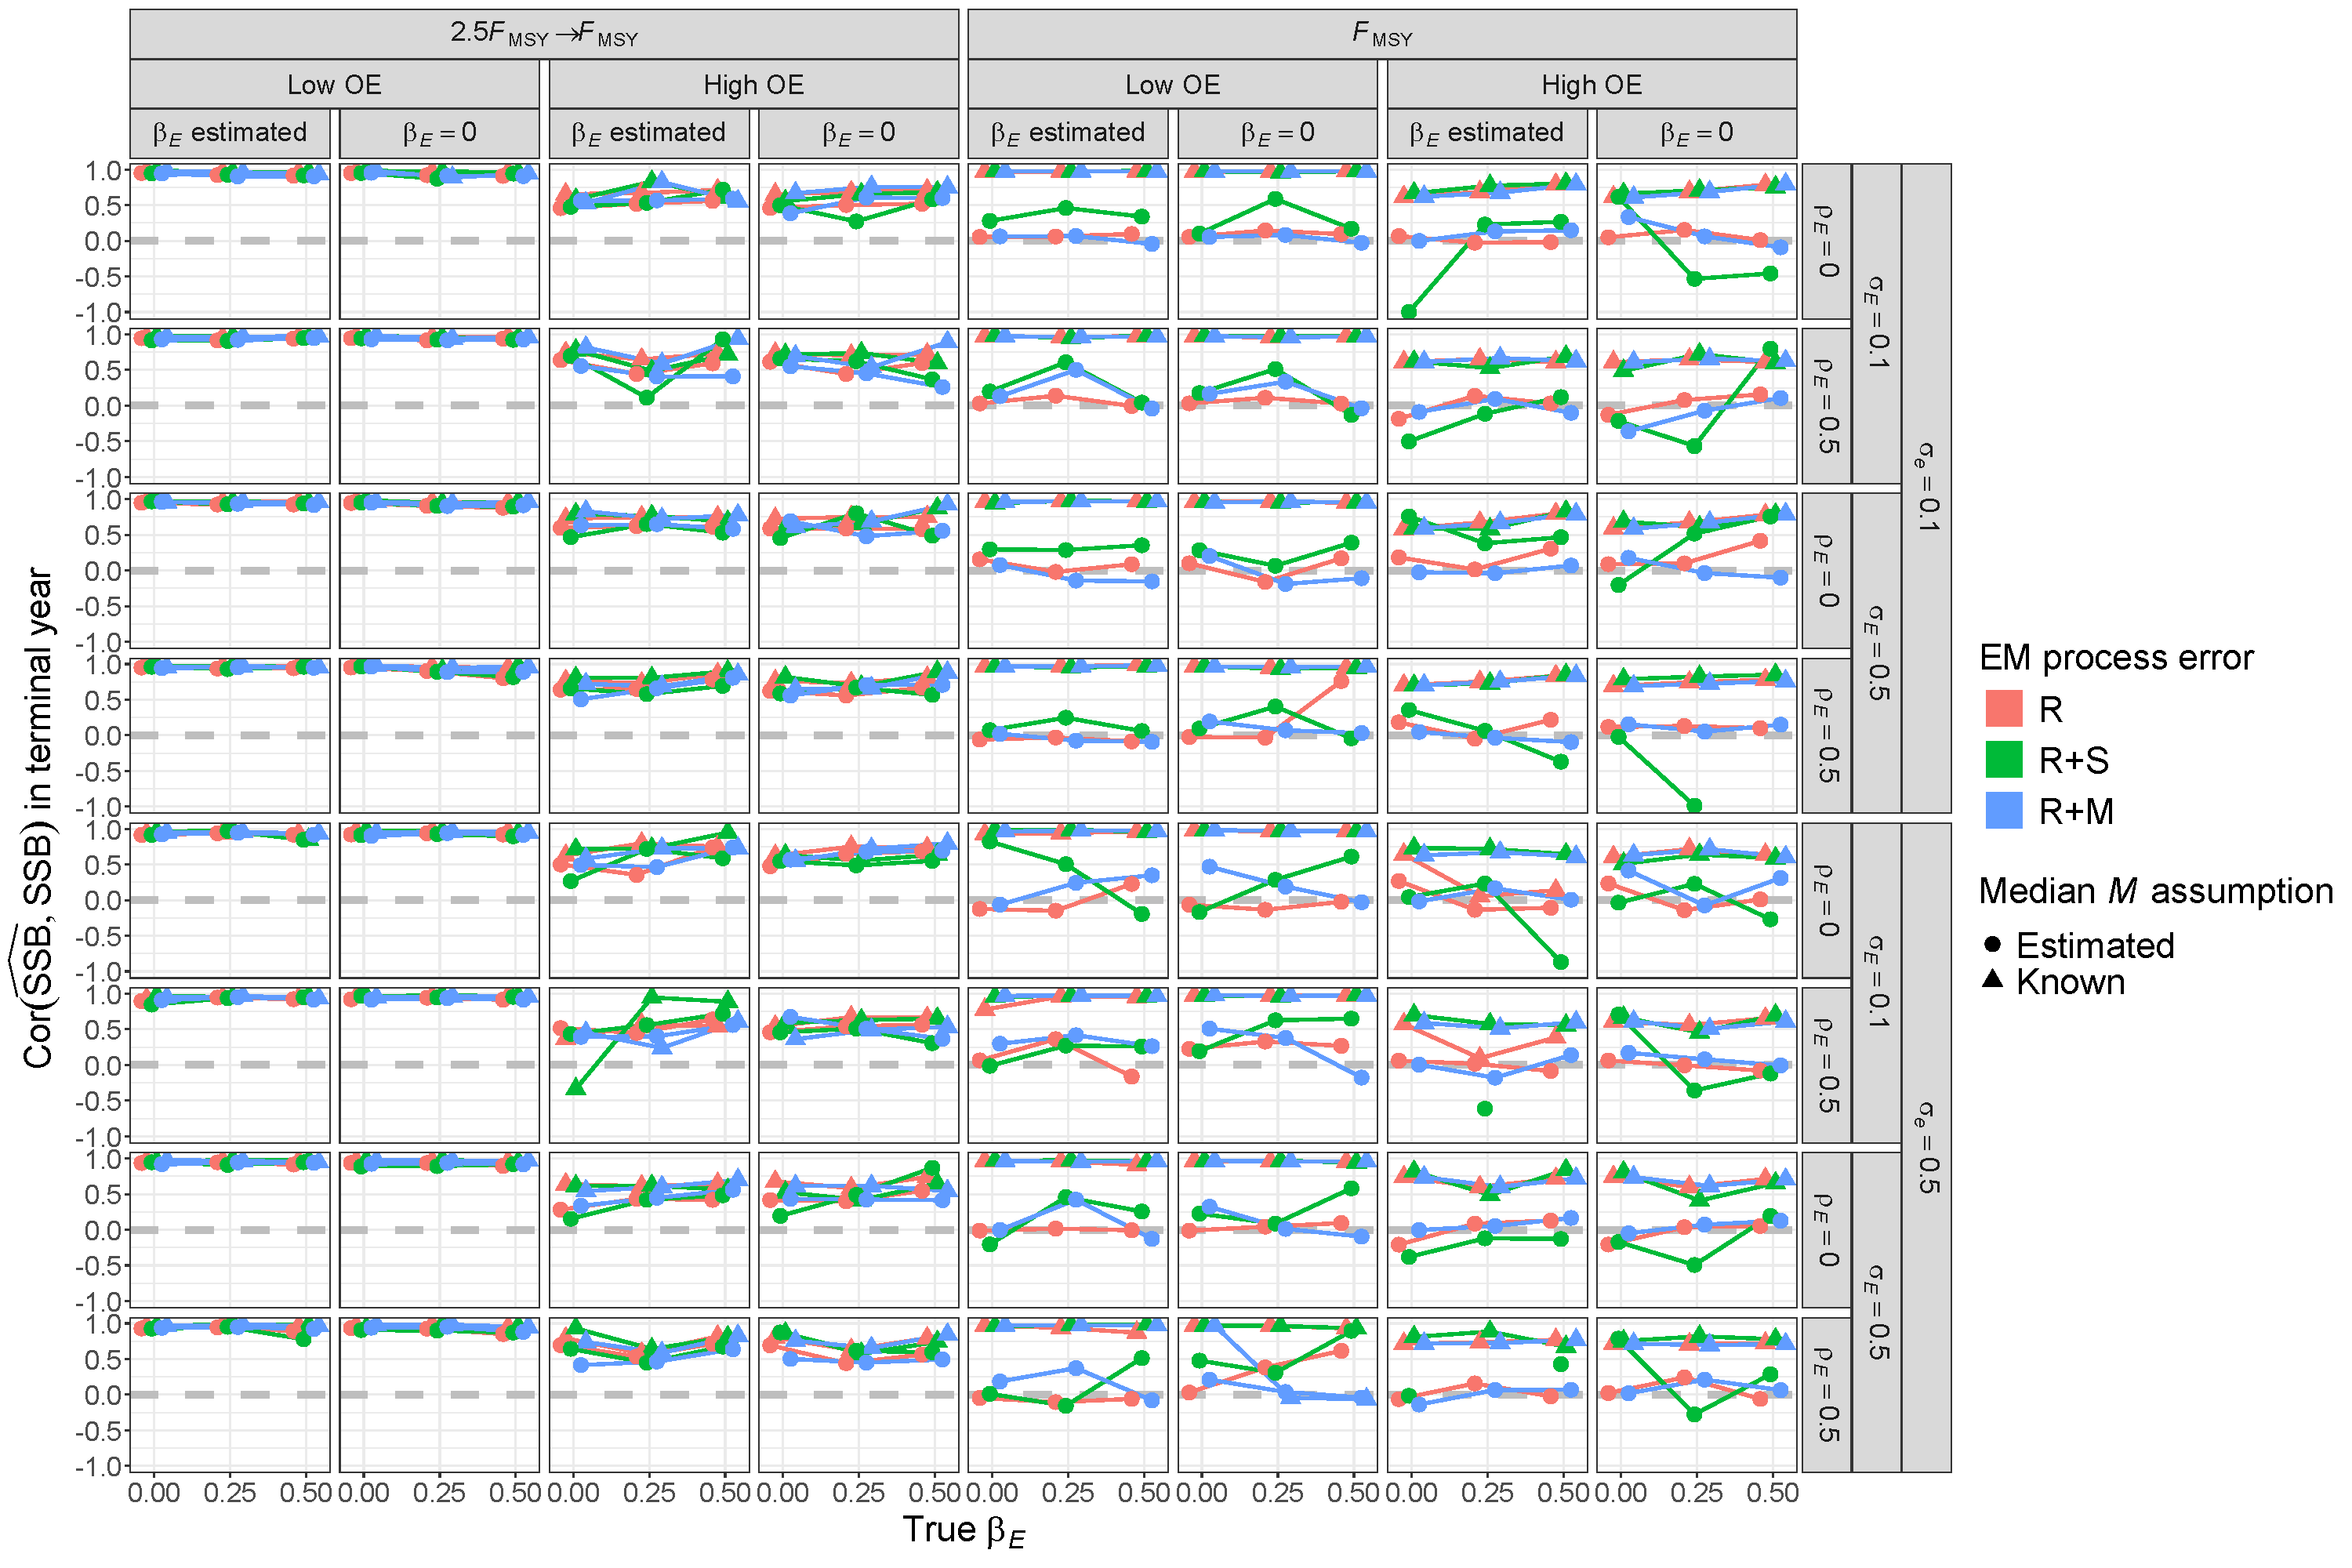
\includegraphics[height = \textheight]{terminal_year_ssb_corr_Rom}
\end{center}
\caption{For R operating models, correlation of estimates and true values of terminal year SSB for estimating models with alternative process error assumptions, treatment of covariate effect ($\beta_E = 0$ or estimated), and treatment of median $M$ parameter ($\beta_M$ estimated or known).}\label{terminal_ssb_corr_Rom}
\end{figure}
\end{landscape}

\begin{landscape}
\begin{figure}
\begin{center}
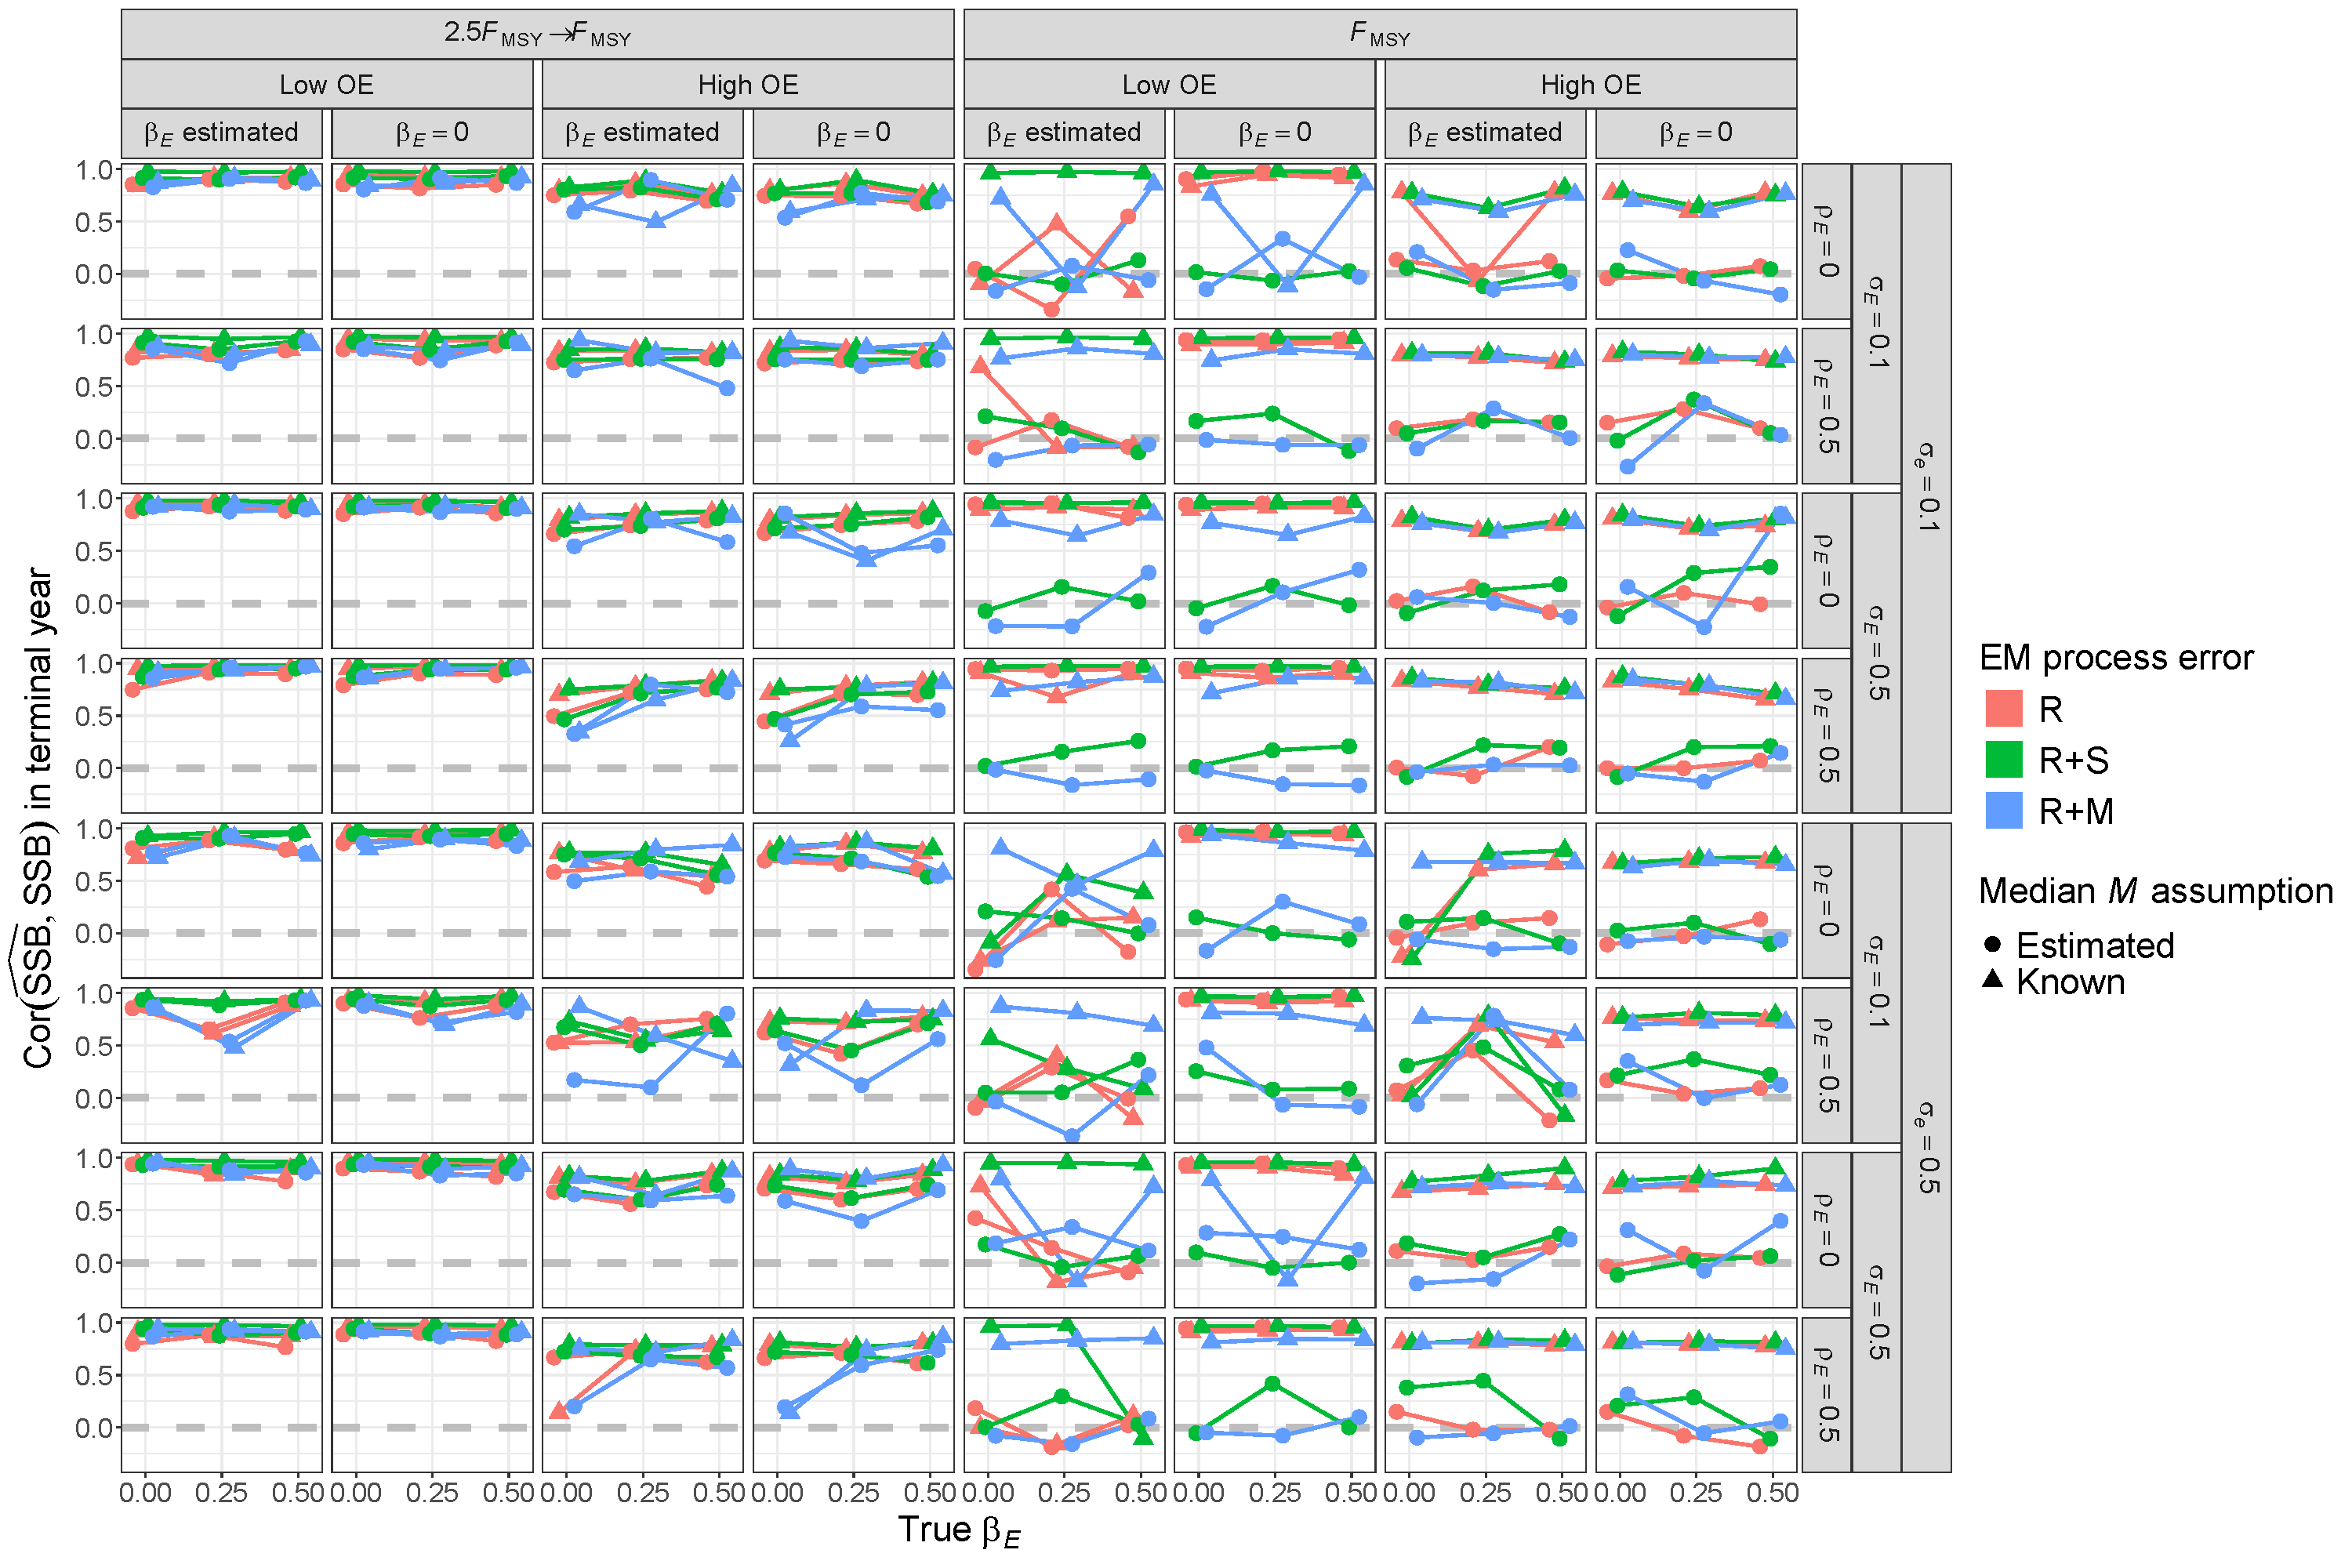
\includegraphics[height = \textheight]{terminal_year_ssb_corr_RSom}
\end{center}
\caption{For R+S operating models, correlation of estimates and true values of terminal year SSB for estimating models with alternative process error assumptions, treatment of covariate effect ($\beta_E = 0$ or estimated), and treatment of median $M$ parameter ($\beta_M$ estimated or known).}\label{terminal_ssb_corr_RSom}
\end{figure}
\end{landscape}

\begin{landscape}
\begin{figure}
\begin{center}
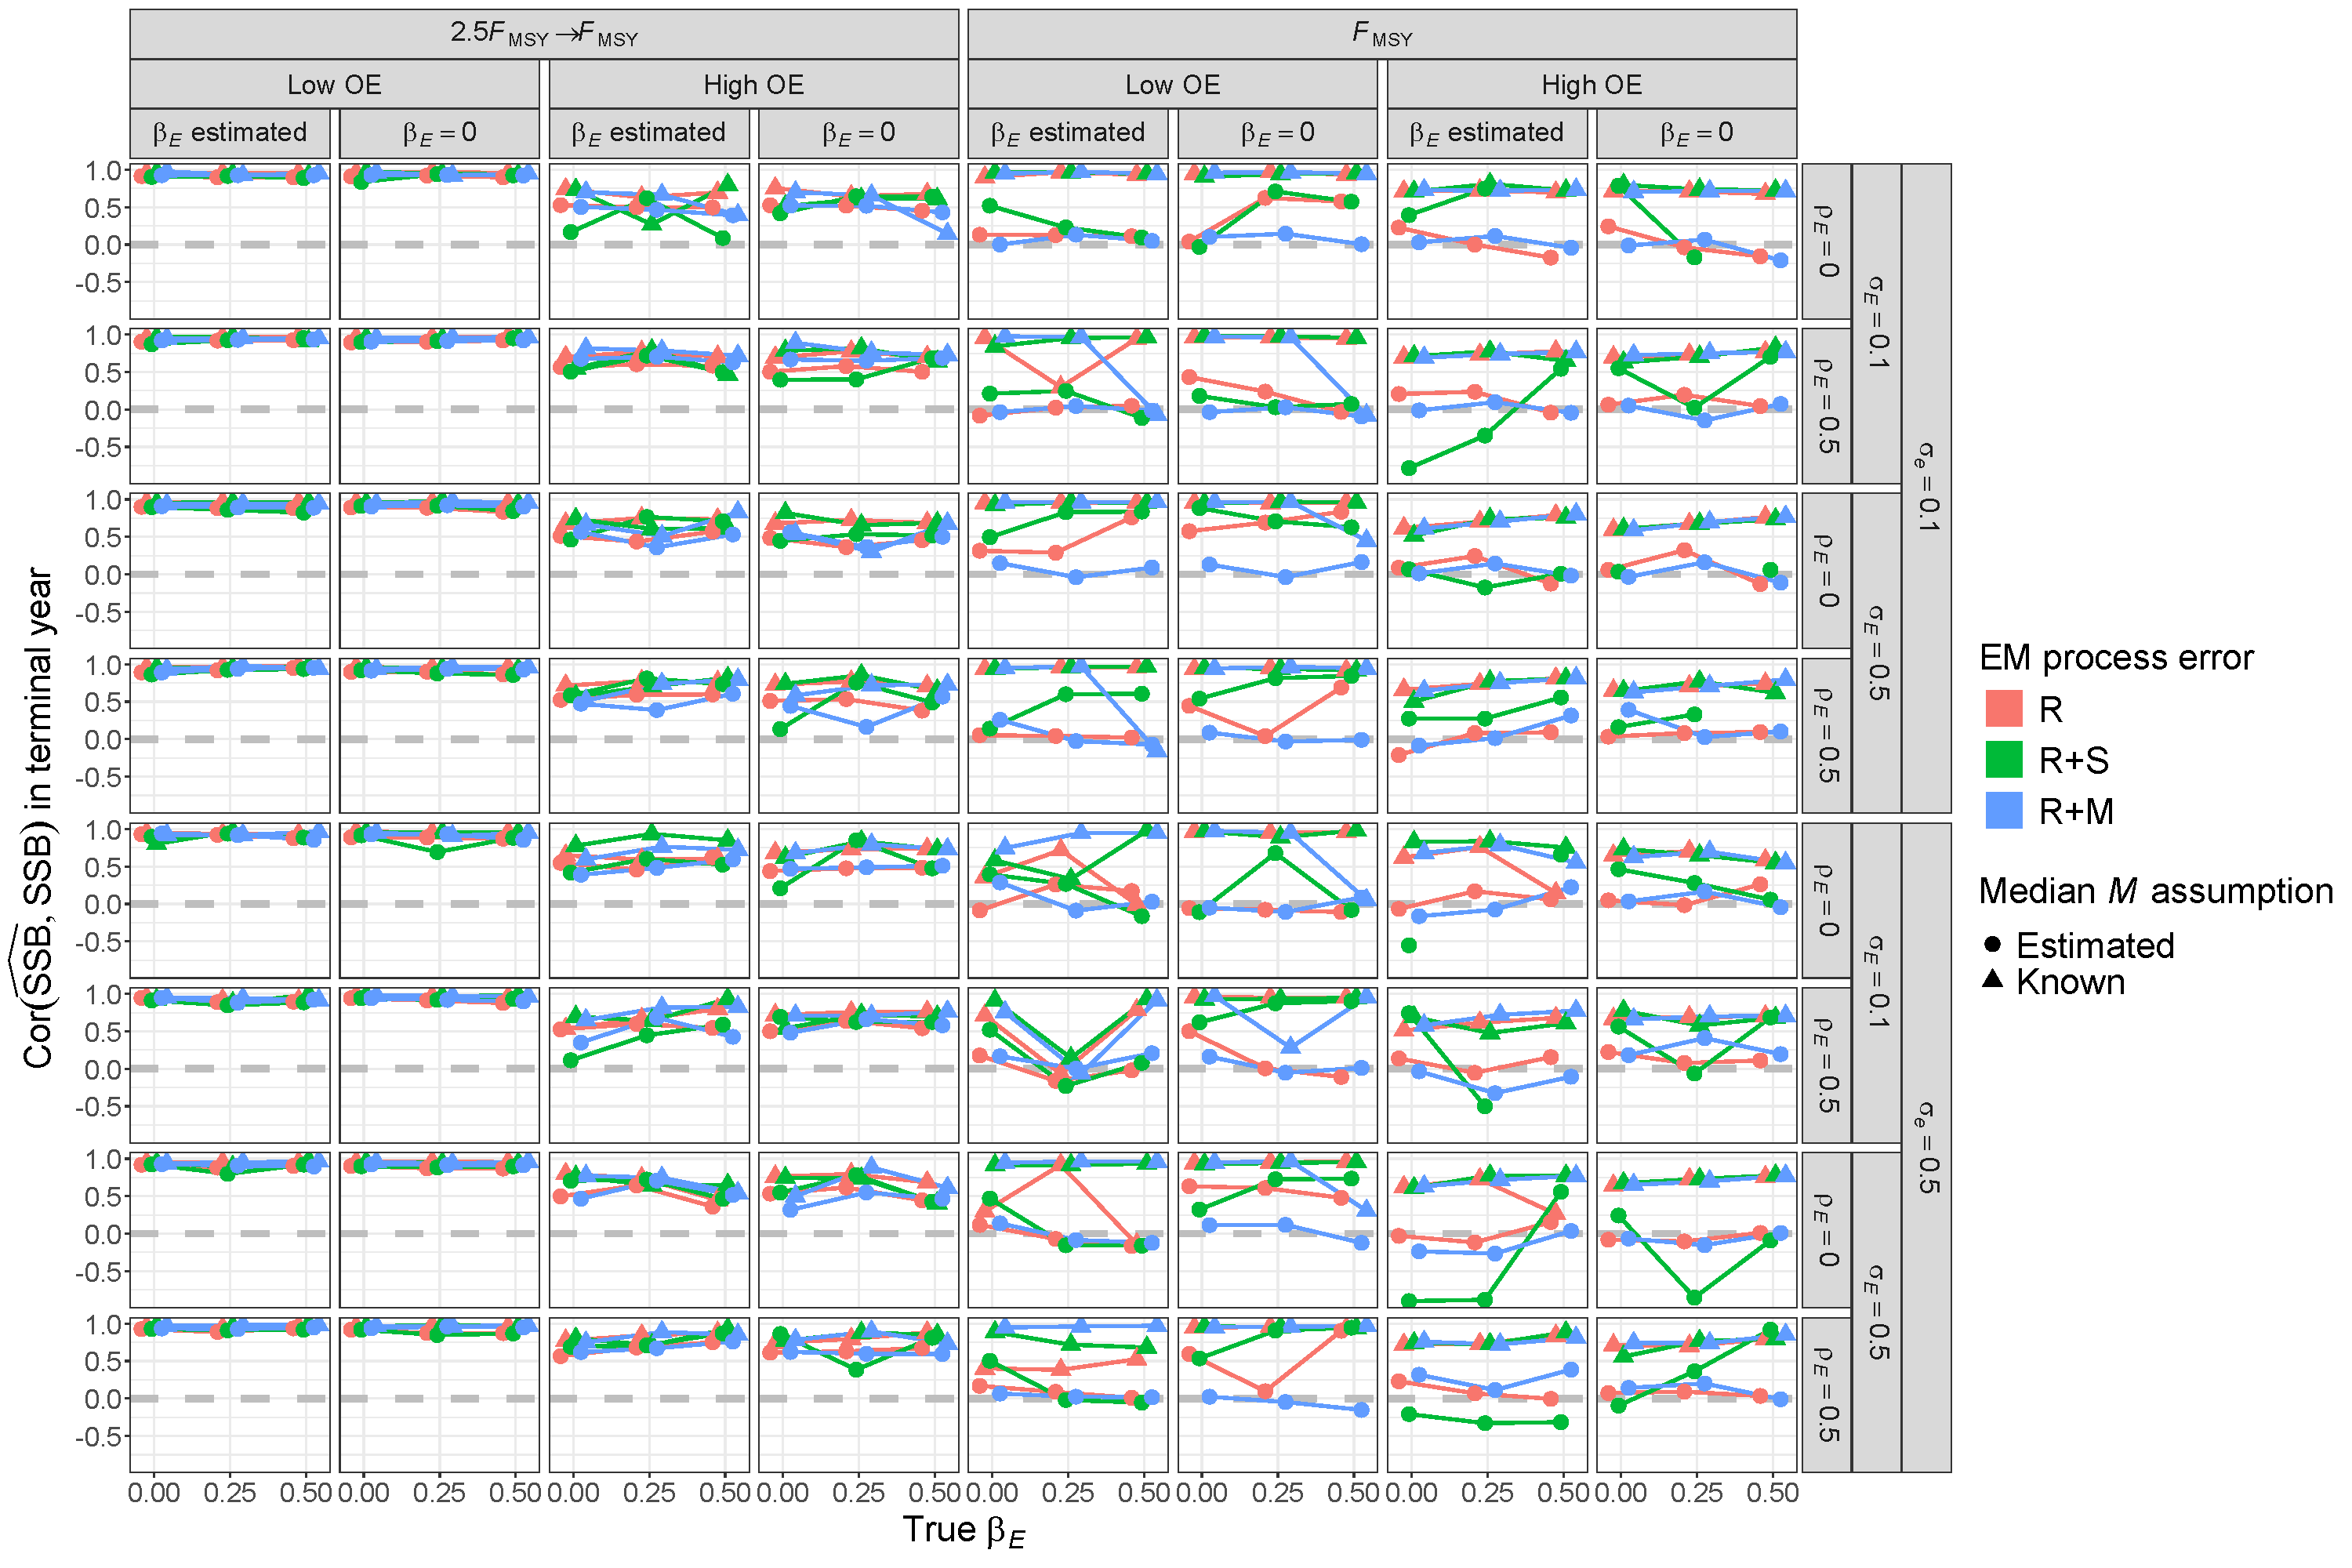
\includegraphics[height = \textheight]{terminal_year_ssb_corr_RMom}
\end{center}
\caption{For R+M operating models, correlation of estimates and true vales of terminal year SSB for estimating models with alternative process error assumptions, treatment of covariate effect ($\beta_E = 0$ or estimated), and treatment of median $M$ parameter ($\beta_M$ estimated or known).}\label{terminal_ssb_corr_RMom}
\end{figure}
\end{landscape}

\begin{landscape}
\begin{figure}
\begin{center}
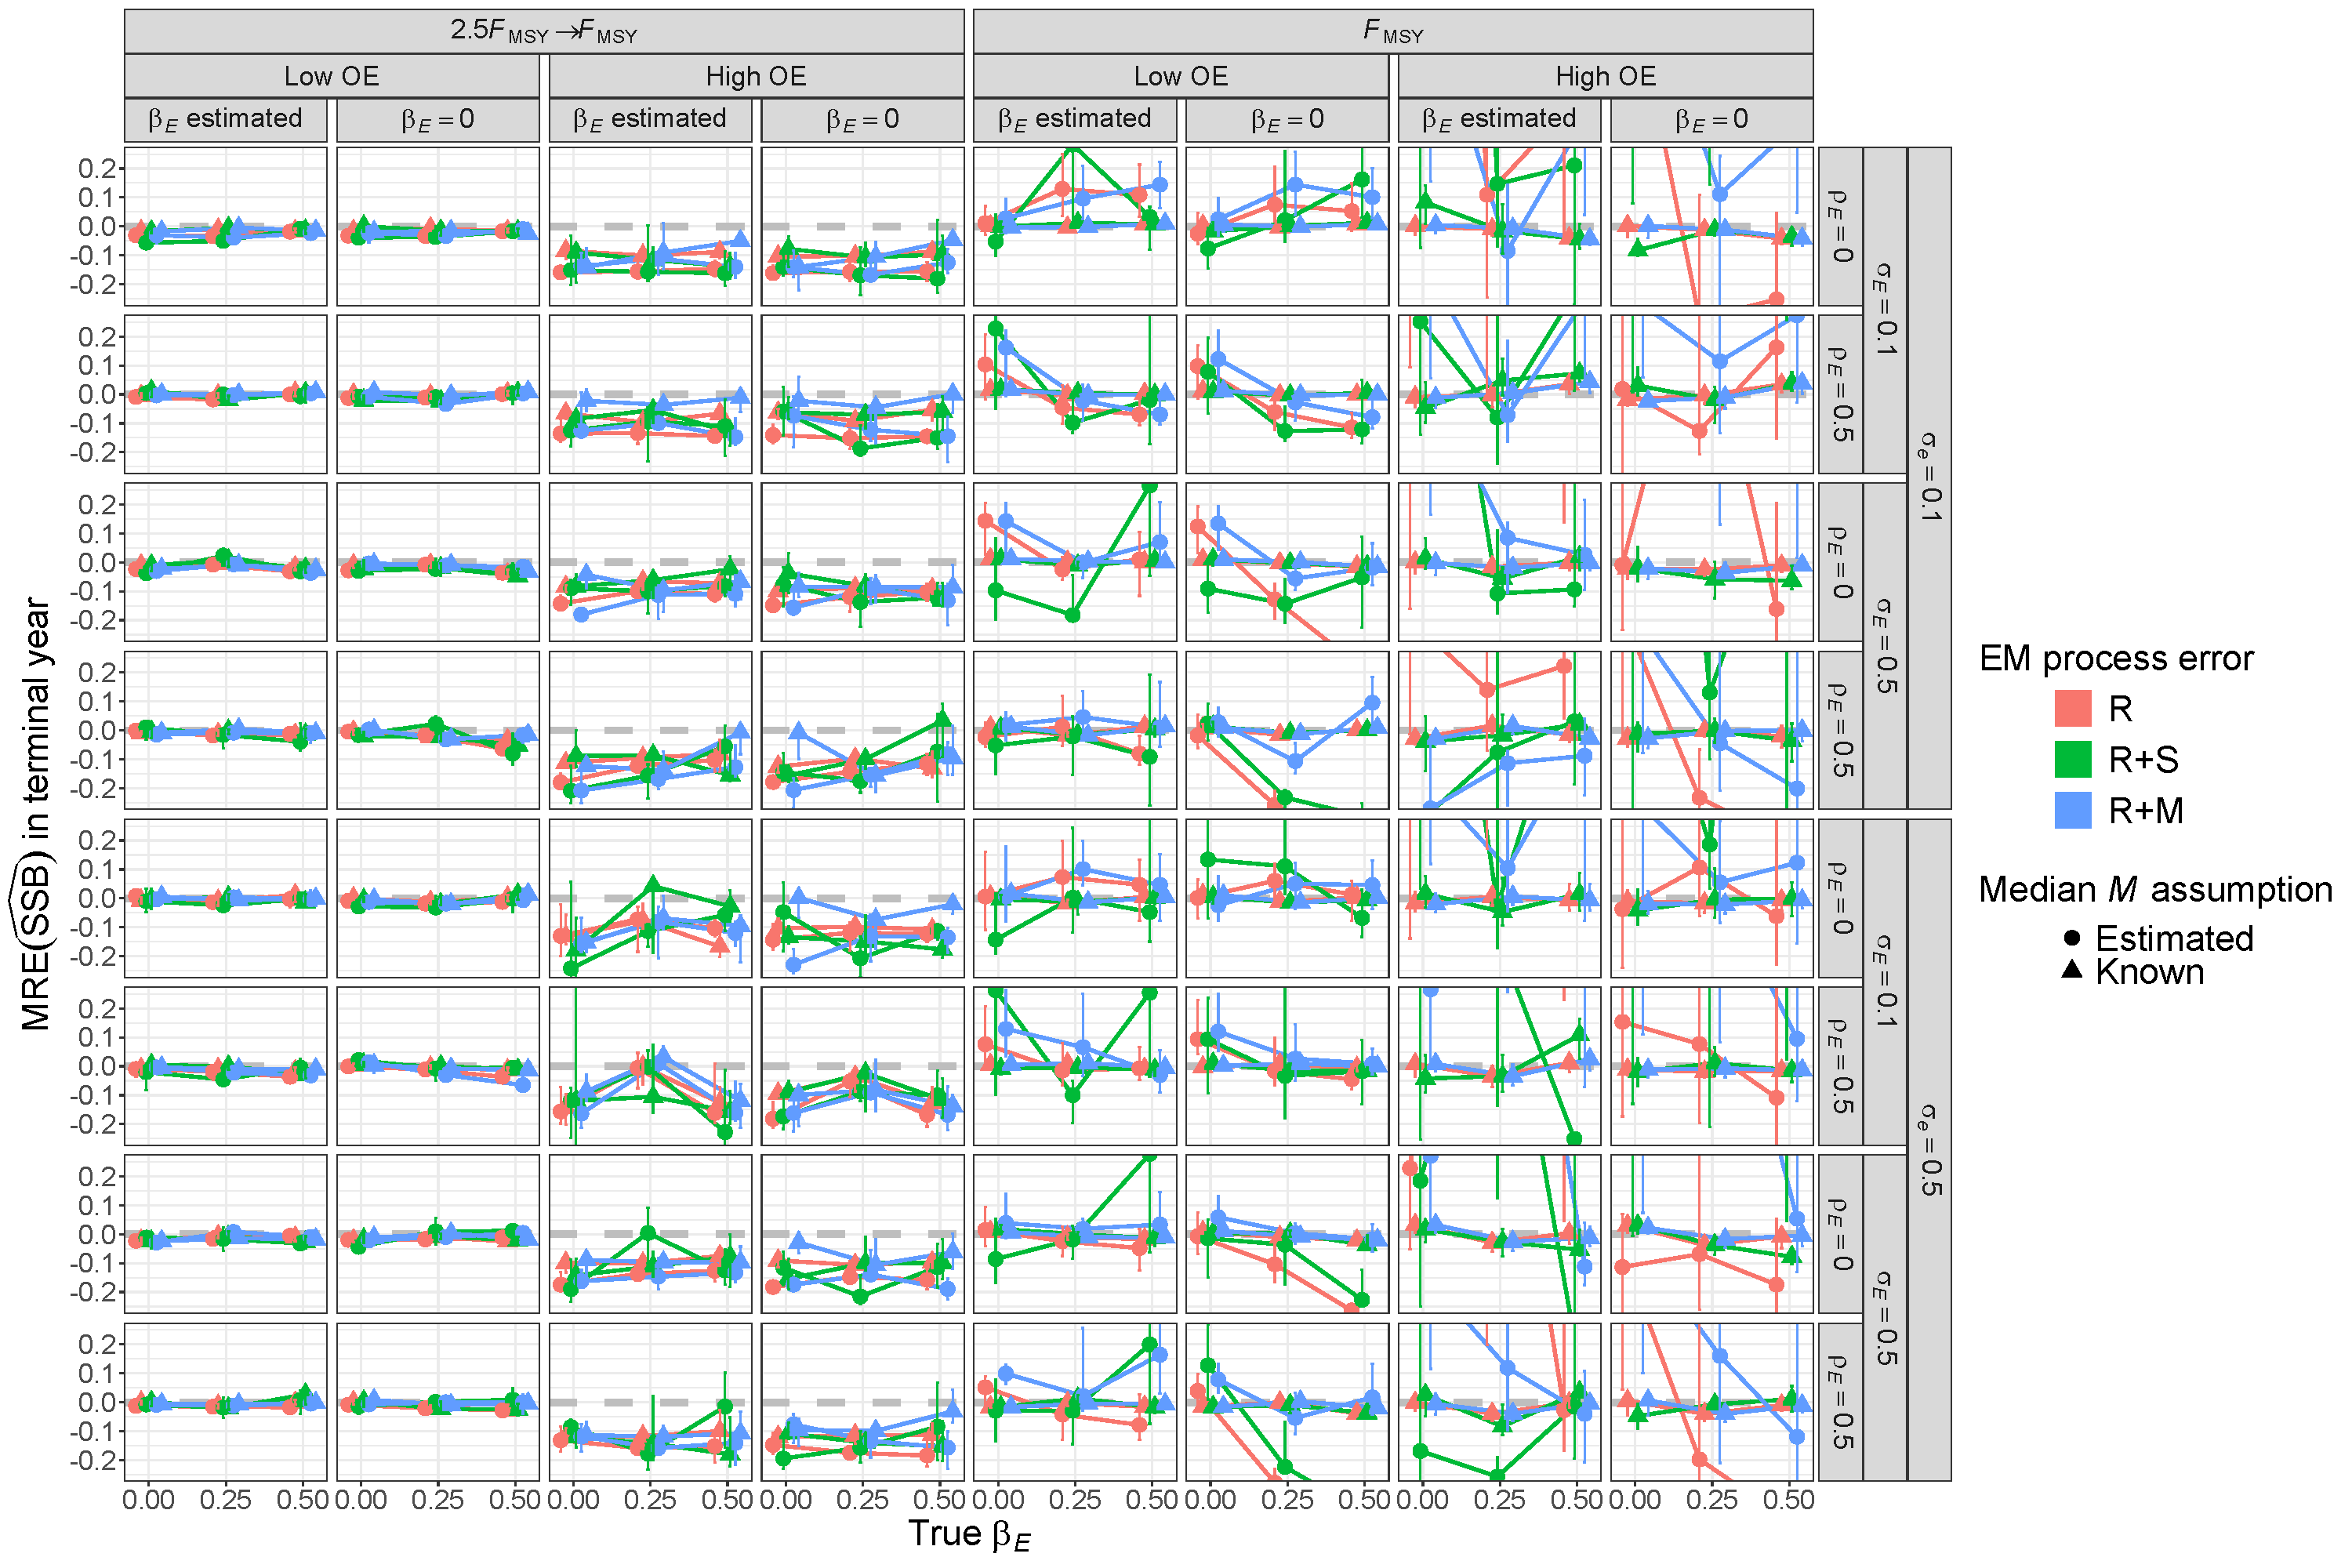
\includegraphics[height = \textheight]{terminal_year_ssb_bias_Rom}
\end{center}
\caption{For R operating models, median relative error (MRE) of estimates of SSB in the terminal year for estimating models with alternative process error assumptions, treatment of covariate effect ($\beta_E = 0$ or estimated), and treatment of median $M$ parameter ($\beta_M$ estimated or known).}\label{terminal_ssb_bias_Rom}
\end{figure}
\end{landscape}

\begin{landscape}
\begin{figure}
\begin{center}
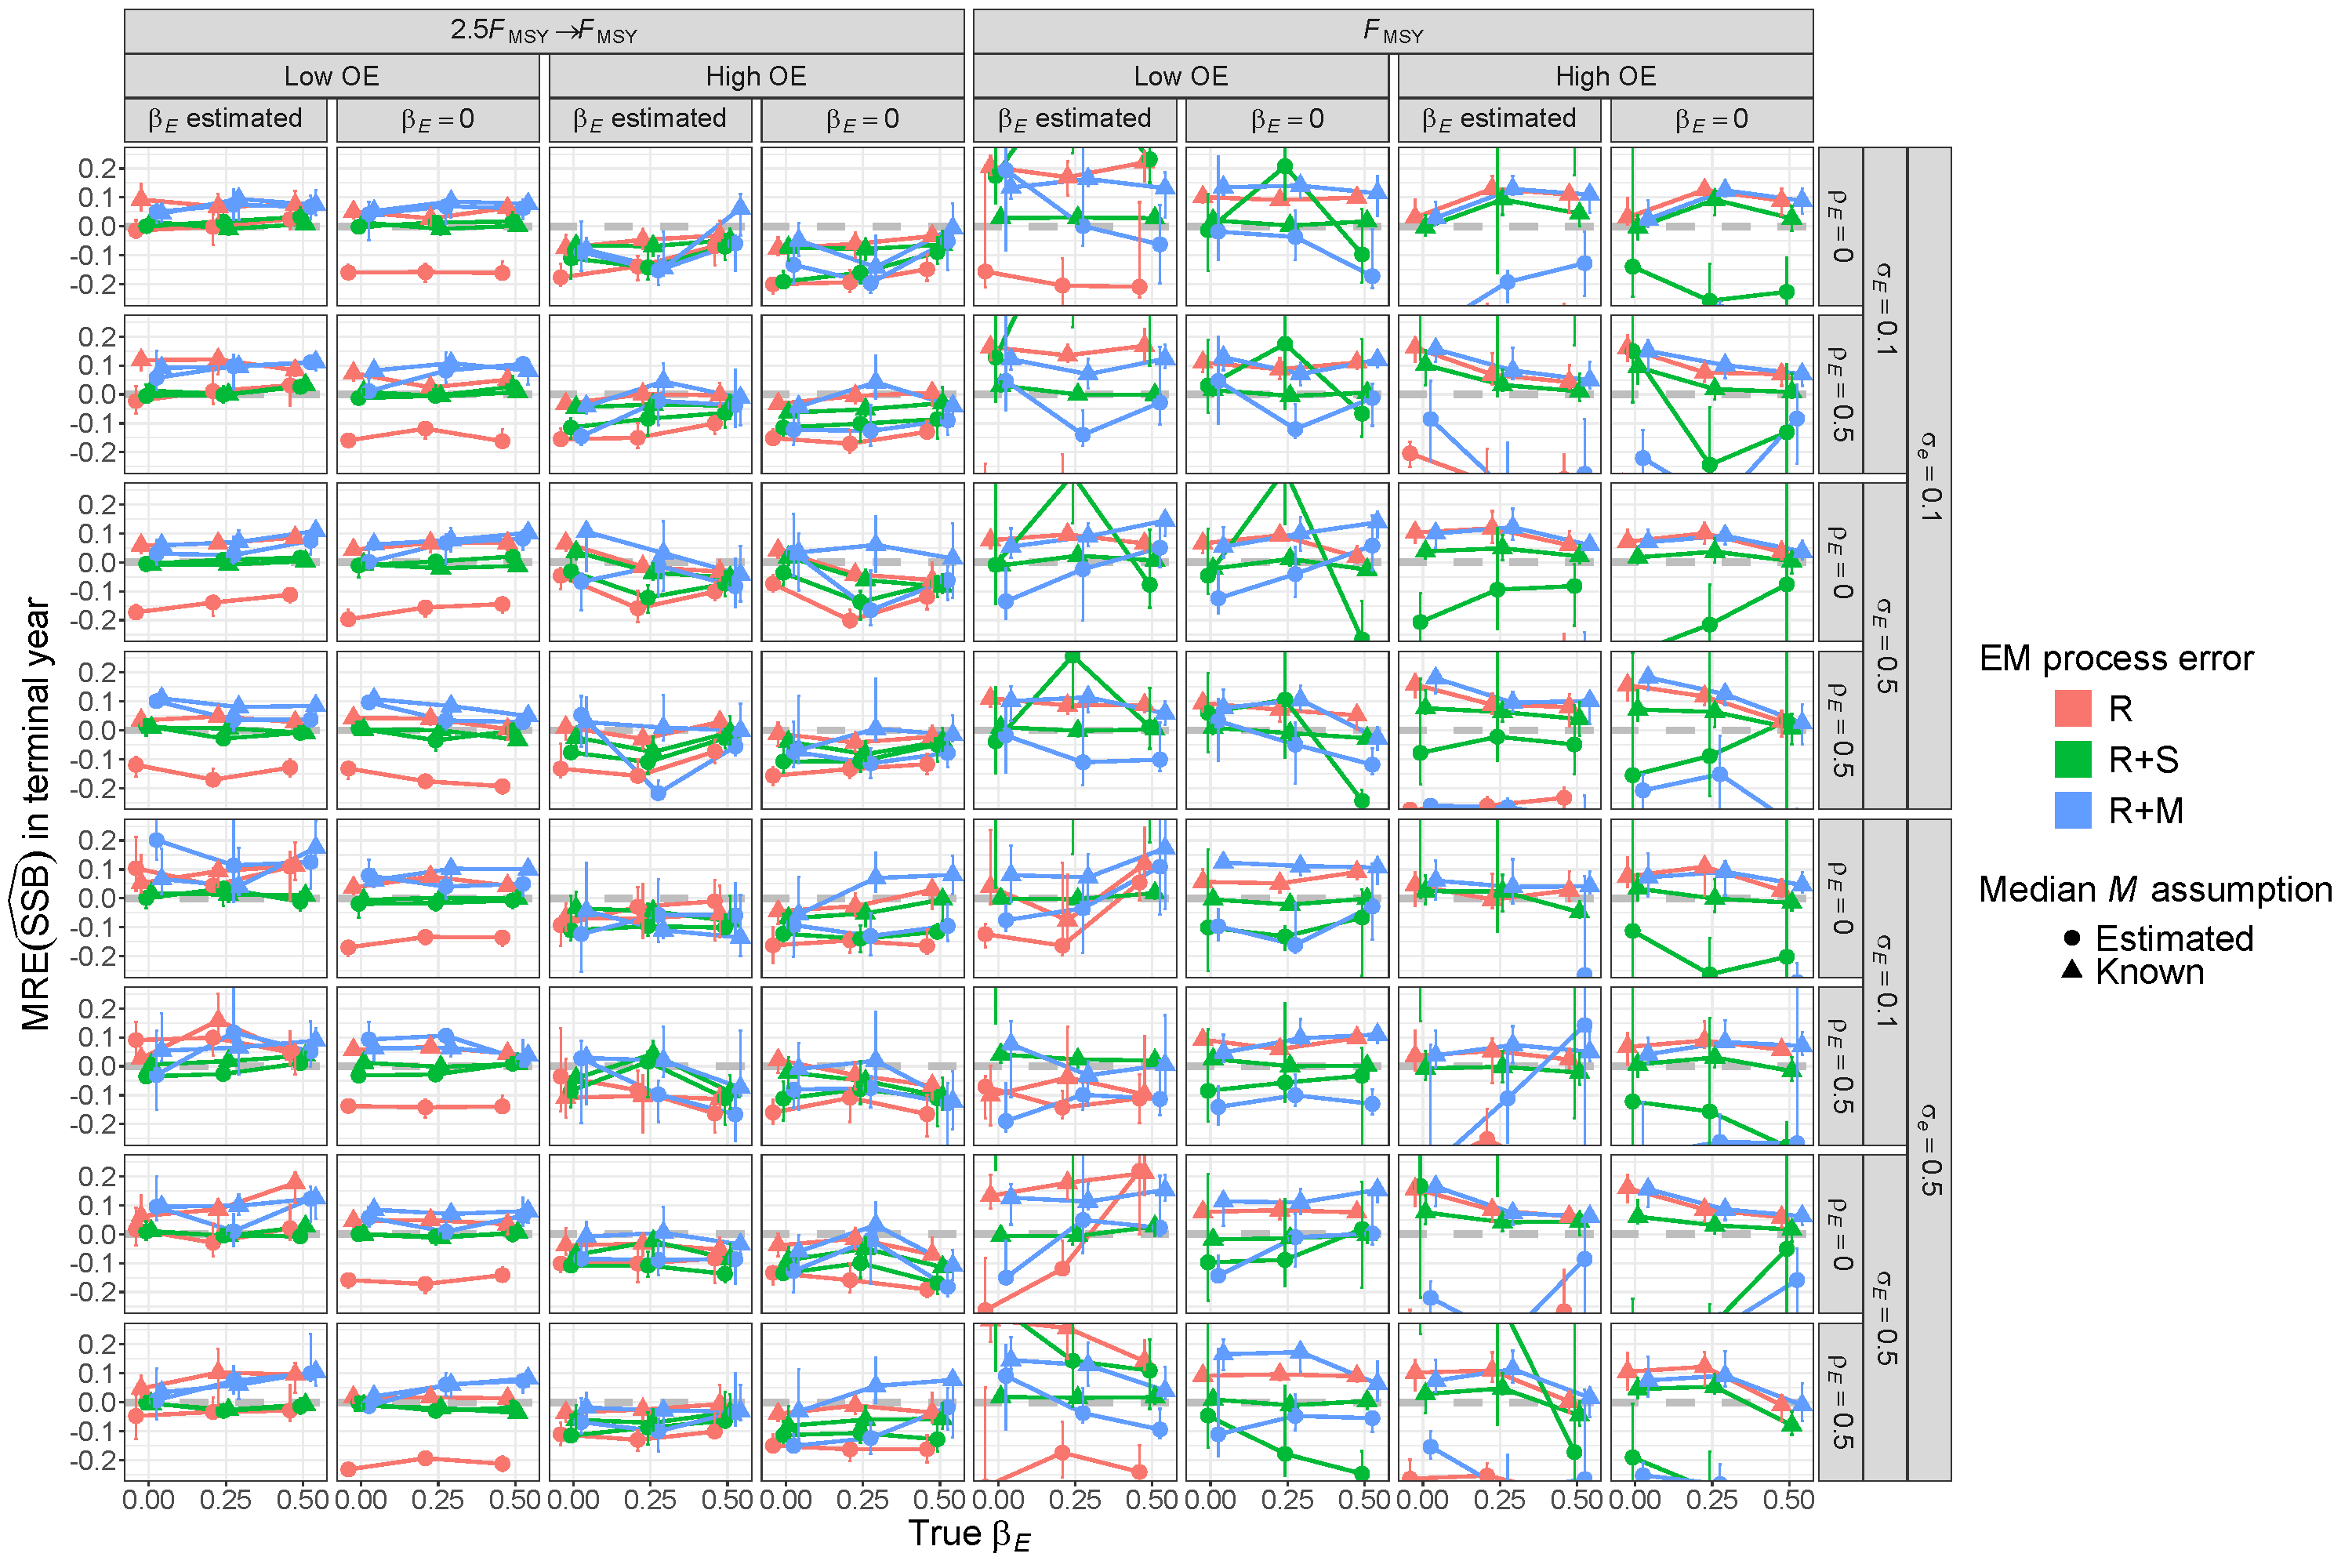
\includegraphics[height = \textheight]{terminal_year_ssb_bias_RSom}
\end{center}
\caption{For R+S operating models, median relative error (MRE) of SSB in the terminal year for estimating models with alternative process error assumptions, treatment of covariate effect ($\beta_E = 0$ or estimated), and treatment of median $M$ parameter ($\beta_M$ estimated or known).}\label{terminal_ssb_bias_RSom}
\end{figure}
\end{landscape}

\begin{landscape}
\begin{figure}
\begin{center}
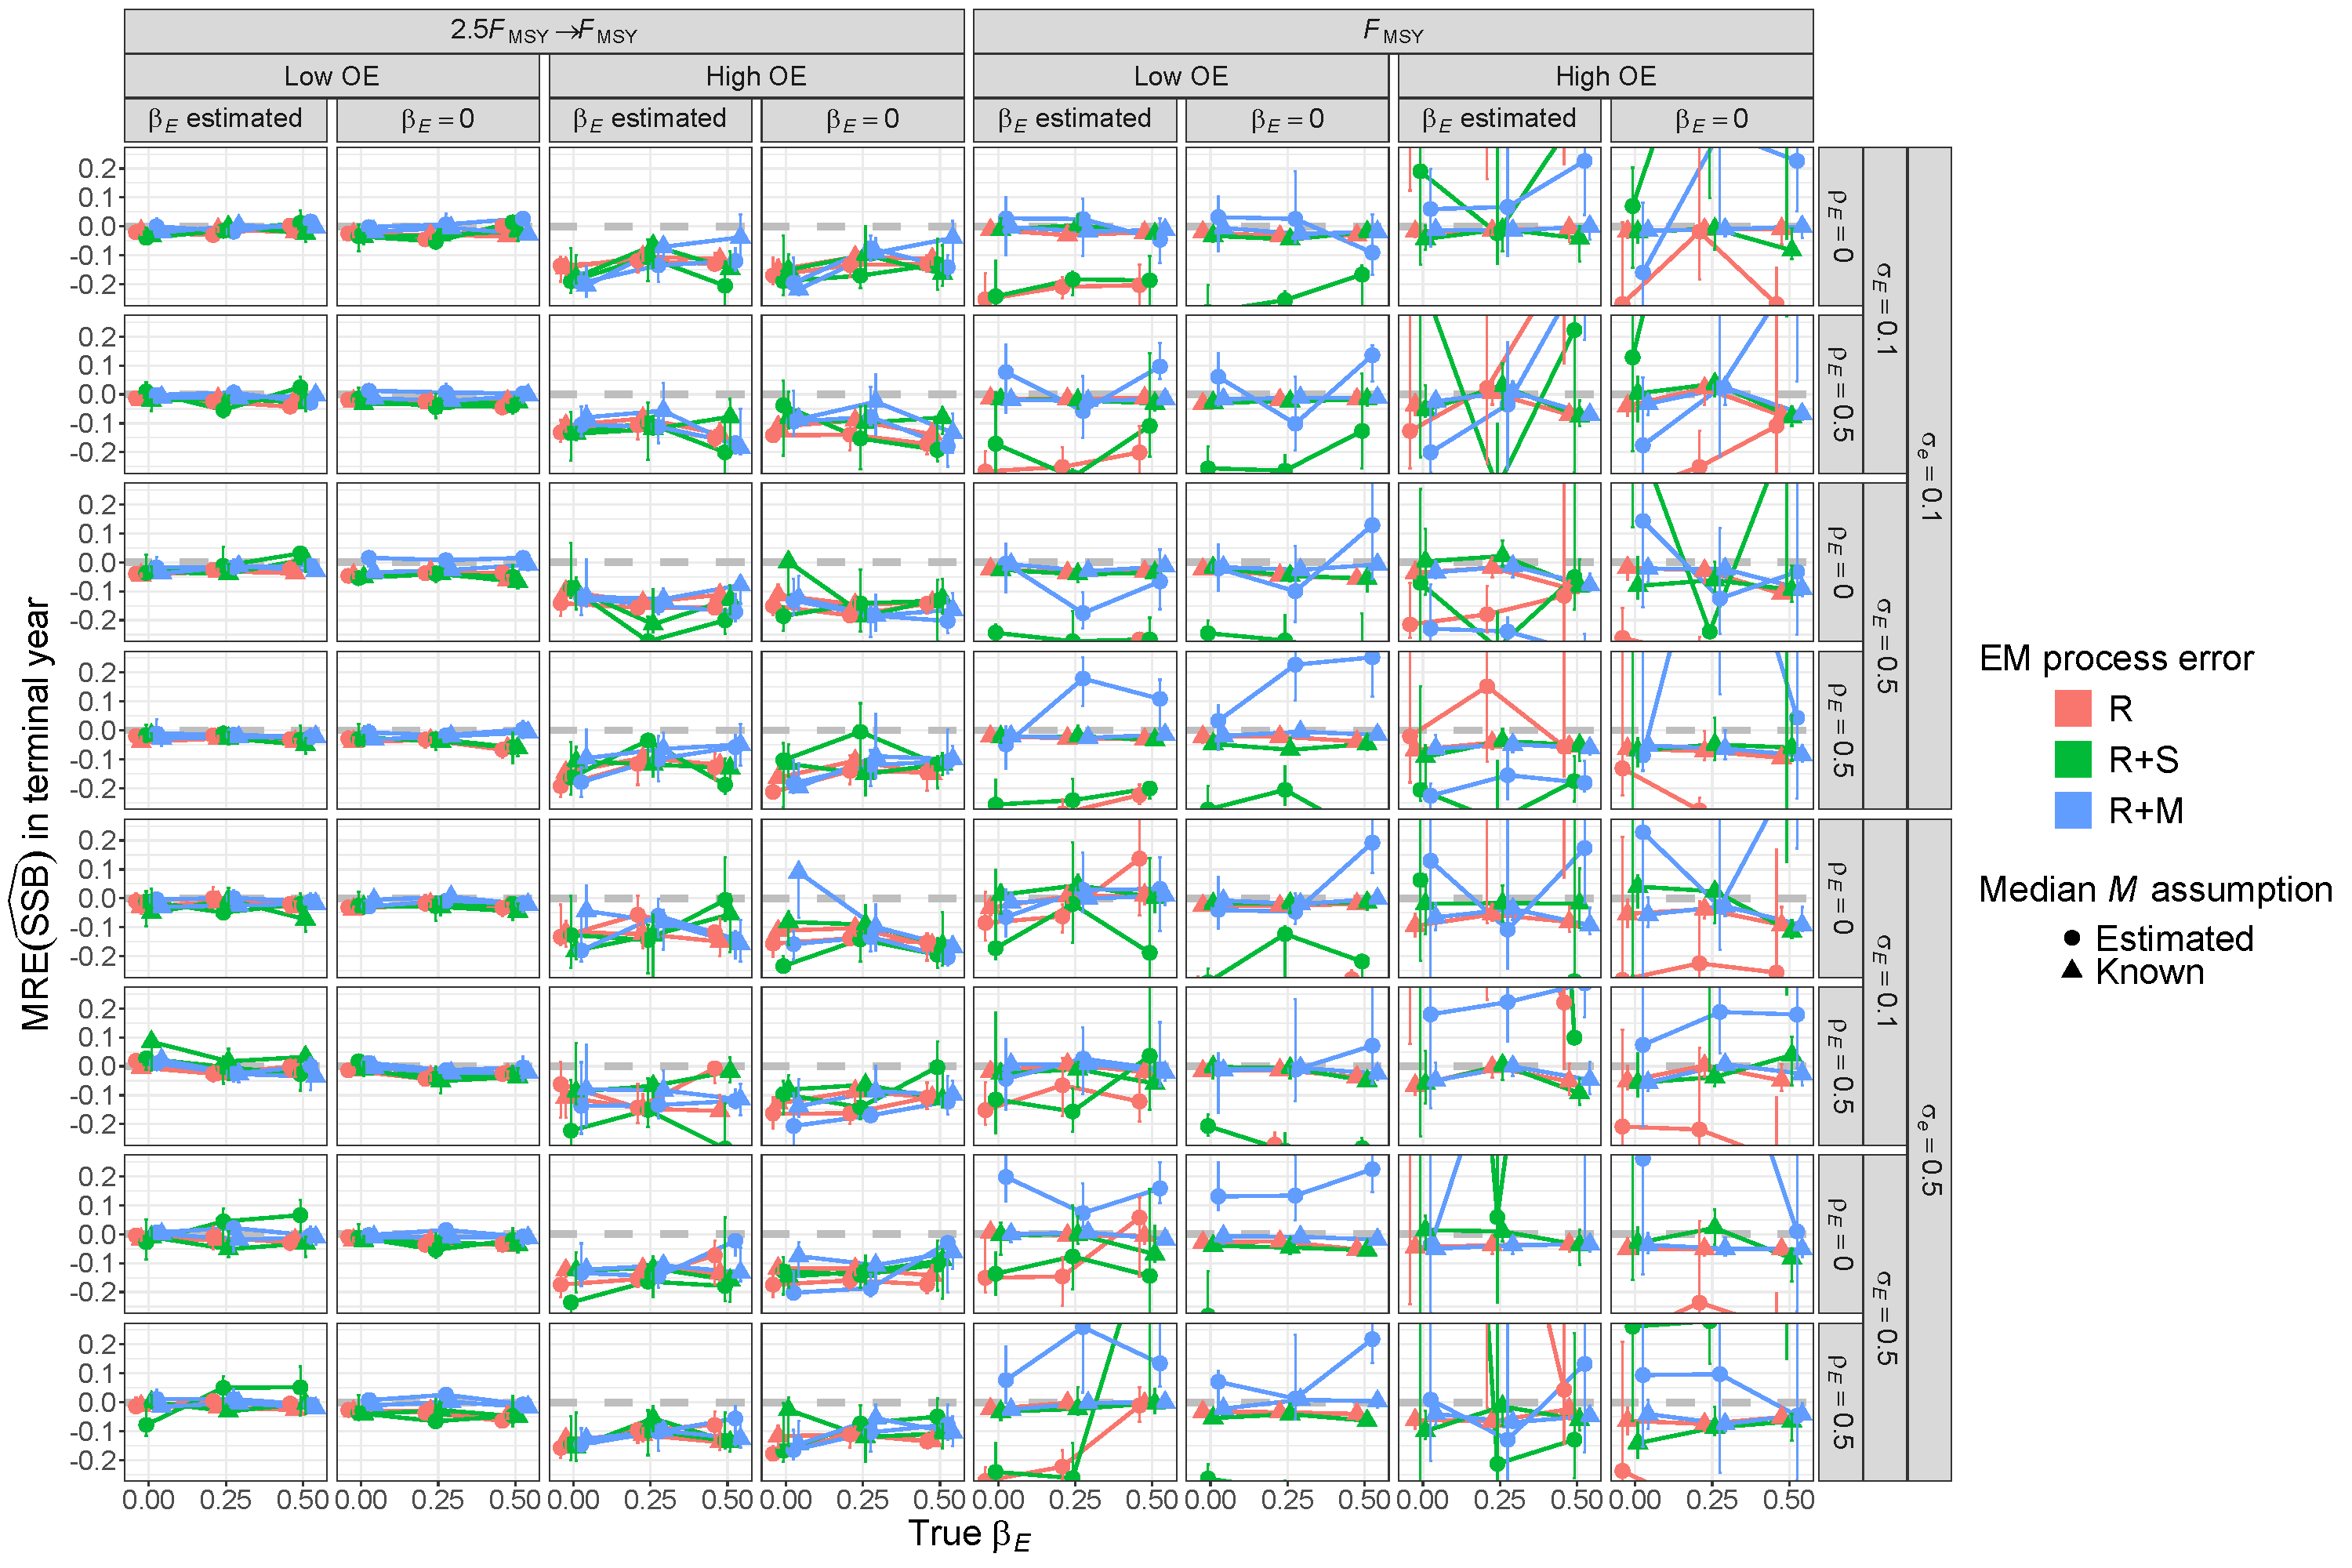
\includegraphics[height = \textheight]{terminal_year_ssb_bias_RMom}
\end{center}
\caption{For R+M operating models, median relative error (MRE) of estimates of SSB in the terminal year for estimating models with alternative process error assumptions, treatment of covariate effect ($\beta_E = 0$ or estimated), and treatment of median $M$ parameter ($\beta_M$ estimated or known).}\label{terminal_ssb_bias_RMom}
\end{figure}
\end{landscape}

\begin{table}
\caption{Operating (OM) and estimating model (EM) attributes used in analyses of deviance reduction and classification and regression trees. R, R+S, and R+M, denote models (OM or EM) with process error on recruitment only, recruitment and apparent survival, and recruitment and natural mortality, respectively. SD denotes standard deviation and \Fmsy is the fishing mortality rate that acheives maximum sustainable yield.}\label{factor_table}
{\input{factor_table}}
\end{table}
\pagebreak

\begin{landscape}
\end{landscape}

\subsection*{Percent deviance reduction
results}\label{percent-deviance-reduction-results}
\addcontentsline{toc}{subsection}{Percent deviance reduction results}

\subsubsection*{Estimating model
convergence}\label{estimating-model-convergence}
\addcontentsline{toc}{subsubsection}{Estimating model convergence}

For fitted logistic regression models to indicators of convergence, the
estimating model process error assumption provided the largest percent
reduction in deviance (9-25\%) of all operating model and estimating
model attributes for all three operating model process error types
(Table \ref{convergence_PRD_table}). Including second order interactions
of operating model and estimating model factors also provided further
reduction of residual deviance (between 7 and 11\%), indicating
successful convergence depended on a combination of operating model and
estimating model attributes.

\subsubsection*{AIC performance of process error source
selection}\label{aic-performance-of-process-error-source-selection}
\addcontentsline{toc}{subsubsection}{AIC performance of process error
source selection}

For all OM process error types, the level of error in both the
population and covariate observations were the attributes that resulted
in the largest percent reductions in deviance for multinomial regression
fits to indicators of AIC selection of the process error configuration
(Table \ref{AIC_PE_PRD_table}). For R+S and R+M OMs, level of error in
population observations provided deviance reduction (19\% and 13\%,
respectively) much larger than any other OM and EM factors whereas error
in covariate observations provided the largest reduction (8\%) for R
OMs. Lesser deviance reduction (2-3\%) occurred for the true covariate
effect size and whether the EM made the correct assumption about
including a covariate effect for R OMs and error in covariate
observations for R+M OMs. Including second and third order interactions,
provided the largest reductions in residual deviance for R OMs (24\%)
and little reduction for R+S and R+M OMs (4\% and 6\%, respectively).

\subsubsection*{AIC performance of covariate effect
selection}\label{aic-performance-of-covariate-effect-selection}
\addcontentsline{toc}{subsubsection}{AIC performance of covariate effect
selection}

The factors explaining the largest reduction in deviance for logistic
regression models fitted to indicators of AIC selection of the correct
covariate effect assumption depended on the magnitude of the true effect
assumed in the OM (Table \ref{AIC_Ecov_effect_PRD_table}). When OMs had
no covariate effect (\(\beta_E = 0\)) the OM process errror type
provided the largest reduction in deviance (4\%). When OMs assumed a
covariate effect (\(\beta_E>0\)), level of error in population
observations and magnitude of temporal variability in the true covariate
provided the largest reductions in deviance (4\% and 8-21\%,
respectively). The reduction in deviance provided by the magnitude of
covariate temporal variability also increased with larger true covariate
effect. Including second and third order interactions provided a modest
reduction in deviance (5-7\%).

\subsubsection*{Median natural mortality rate
bias}\label{median-natural-mortality-rate-bias}
\addcontentsline{toc}{subsubsection}{Median natural mortality rate bias}

Across all OM process error types, regression models fit to errors in
\(\widehat \beta_M\) showed largest reductions in deviance from the type
of OM fishing pressure (4-17\%), EM process error assumption (2-12\%),
and the EM covariate effect assumption (3-7\%, Table
\ref{bias_median_M_converged_PRD_table}). The level of observation error
also provided a similar reduction in deviance for R OMs (3\%).
Relatively large reductions in deviance also occurred with second and
third order interactions (7-16\%).

\subsubsection*{Median natural mortality rate standard error
bias}\label{median-natural-mortality-rate-standard-error-bias}
\addcontentsline{toc}{subsubsection}{Median natural mortality rate
standard error bias}

The EM process error assumption provided the largest reduction in
deviance for regression models fitted to errors in
\(\widehat {\text{SE}}\left(\widehat \beta_M\right)\) from R (3\%) and
R+M (7\%) OM simulations (Table \ref{median_M_se_bias_PRD_table}). The
type of OM fishing pressure provided the largest reduction (13\%) for
R+S OMs and a lesser reduction in devaince for R+M OMs (4\%). The EM
covariate effect assumption also provided similar reductions in deviance
for R+S (9\%) and R+M (4\%) OMs.

\subsubsection*{Median natural mortality rate confidence interval
bias}\label{median-natural-mortality-rate-confidence-interval-bias}
\addcontentsline{toc}{subsubsection}{Median natural mortality rate
confidence interval bias}

For logistic regressions of indicators of CIs including \(\beta_M\),
factors that provided the largest reductions in deviance were the OM
fishing history and level of error in population observations for all OM
process error types (0.3-6\%) (Table
\ref{mean_M_ci_coverage_PRD_table}). Including second and third order
interactions provided the largest relative increase in deviance
reduction for R+S (8-11\%) and R+M OMs (5-8\%) and lesser increases for
R OMs (3-5\%).

\subsubsection*{Covariate effect bias}\label{covariate-effect-bias}
\addcontentsline{toc}{subsubsection}{Covariate effect bias}

For regression models fit to errors in estimation of \(\beta_E\), we
found very little reduction in deviance for any of the OM and EM factors
(Table \ref{bias_ecov_beta_converged_PRD_table}). For the normal model
in these regressions, deviance is the sum of squares and there were
extremely large estimates of \(\beta_E\) (and errors) for many
simulations which resulted in extremely large sums of squares and
relative differences from the null model were therefore small
(\textless1\%). Nevertheless, observation error of the covariate
provided either the largest or second largest reductions in deviance of
any of the single OM and EM attributes for OM process error
configuration types. OM fishing history provided reductions of similar
scale for R and R+S OMs. Other factors providing similar reductions were
true covariate effect size for R OMs and level of error in population
observations and EM process error assumption for R+S OMs. Including
second and third order interactions also provided further reductions in
residual deviance similar in scale to the individual factors.

\subsubsection*{Covariate effect standard error
bias}\label{covariate-effect-standard-error-bias}
\addcontentsline{toc}{subsubsection}{Covariate effect standard error
bias}

Factors providing the largest reductions in deviance for estimation
error of \(\widehat {\text{SE}}\left(\widehat\beta_E\right)\) were
generally similar to those that were most important for estimation of
\(\beta_E\), but deviance reductions were one or two orders of magnitude
larger (Table \ref{bias_ecov_beta_se_PRD_table}). Level of error in
covariate observations and EM process error assumption was important for
all OM process error configurations (6-13\% and 3-4\%, respectively).
Level of error in population observations provided relatively large
reductions in deviance for R+S and R+M OMs (3\% and 8\%, respectively).
The OM fishing pressure history provided a lesser reduction in deviance
for all OM process error types (2-4\%). Like estimation of \(\beta_E\),
additional large reductions in deviance also occurred when second and
third order interactions of OM and EM attributes were included in the
regression models (11-31\%).

\subsubsection*{Covariate effect confidence interval
bias}\label{covariate-effect-confidence-interval-bias}
\addcontentsline{toc}{subsubsection}{Covariate effect confidence
interval bias}

For logistic regressions of indicators of CIs including the true value
of \(\beta_E\), factors that provided the largest reductions in deviance
were true covariate effect size for R and R+M OMs (11\% and 3\%,
respectively) and EM process error configuration for R+S OMs (7\%)
(Table \ref{ecov_beta_ci_coverage_PRD_table}). Covariate observation
error also provided relatively large reduction in deviance for R OMs
(8\%). Lesser reductions of 1-2\% occurred for level of error in
population observations and covariate temporal variability for all OM
process error types. Including second and third order interactions also
provided relatively large further reductions in deviance (5-9\%).

\subsubsection*{Terminal year natural morality rate
bias}\label{terminal-year-natural-morality-rate-bias}
\addcontentsline{toc}{subsubsection}{Terminal year natural morality rate
bias}

Regressions of estimation errors show largest reductions in deviance
from whether the EM treats \(\beta_M\) as known (Table
\ref{bias_M_PRD_table}). For R and R+S OMs, annual \(M\) was constant,
and therefore, terminal \(M\) was known when the true \(\beta_M\) was
assumed known and there will be no error in any of those EMs. Beyond the
\(\beta_M\) assumption, the OM fishing history, level of error in
population observations, and EM assumptions for covariate effect and
process error all provided notable deviance reductions.

\subsubsection*{Terminal year natural morality rate
accuracy}\label{terminal-year-natural-morality-rate-accuracy}
\addcontentsline{toc}{subsubsection}{Terminal year natural morality rate
accuracy}

Like bias of terminal year \(M\), the EM assumption for \(\beta_M\)
provided the largest reduction in deviance (22-45\%) for accuracy as
measured by RMSE for all OM process error types (Table
\ref{rmse_M_PRD_table}). Including second and third order interactions
also provided large further reductions in deviance (21-38\%).

Using correlation to measure accuracy of terminal year \(M\) estimation
provides a different perspective. Treatment of \(\beta_M\) provided
relatively large reductions in deviance for all OM process error types
(3-12\%), but level of variability in the covariate was equally or more
important (3-15\%) as was whether the covariate effect was included in
the EM (12\%) for R and R+S OMs (Table \ref{corr_M_PRD_table}).
Including second and third order interactions also provided relatively
large ruther reductions in deviance (15 to 24\%).

\subsubsection*{Terminal year spawning stock biomass
bias}\label{terminal-year-spawning-stock-biomass-bias}
\addcontentsline{toc}{subsubsection}{Terminal year spawning stock
biomass bias}

Regression model fits showed largest reductions in deviance for OM
fishing history (2-3\%), error in population observations (1\% for R and
R+M OMs), and EM \(\beta_M\) assumption (2\%; Table
\ref{bias_SSB_PRD_table}). The type of EM process error assumed also
provided a deviance reduction similar in scale for R+S OMs (1\%).
Including second and third order interactions of OM and EM attributes
provided further deviance reductions of 5-10\%.

\subsubsection*{Terminal year spawning stock biomass
accuracy}\label{terminal-year-spawning-stock-biomass-accuracy}
\addcontentsline{toc}{subsubsection}{Terminal year spawning stock
biomass accuracy}

Largest reductions in deviance were provided by whether \(\beta_M\) was
known or estimated (20-21\%) and whether there was temporal contrast in
fishing pressure (20-33\%) across all OM process error types (Table
\ref{rmse_SSB_PRD_table}). Lesser reductions were also provided by the
EM process error assumption for R and R+M OMs. Inclusion of second and
third order interactions of OM and EM attributes provided further
reductions in deviance of 26-40\%.

Using correlation to measure accuracy, temporal contrast in fishing
pressure and EM treatment of \(\beta_M\) provided relatively important
reductions in deviance like RMSE, but level of error in population
observations was important rather than EM process error type (Table
\ref{corr_ssb_PRD_table}). Including second and third order interactions
also provided relatively large ruther reductions in deviance (6 to
20\%).

\begin{table}
\caption{Percent reduction in deviance for logistic regression models fit to indicators of convergence (providing Hessian-based standard errors). Table rows give each operating model (OM) and estimating model (EM) factor included individually, combined, and with second and third order interactions. Table columns categorize operating models (OMs) with process error on recruitment only (R), recruitment and apparent survival (R+S), or recruitment and natural mortality (R+M). See Table \ref{factor_table} for further details.}\label{convergence_PRD_table}
{\input{convergence_PRD_table}}
\end{table}
\pagebreak

\begin{table}
\caption{Percent reduction in deviance for multinomial logistic regression models fit to indicators of process error assumption in the estimating models with lowest AIC. See Tables \ref{convergence_PRD_table} and \ref{factor_table} for further details.}\label{AIC_PE_PRD_table}
{\input{AIC_PE_PRD_table}}
\end{table}
\pagebreak

\begin{table}
\caption{Percent reduction in deviance for logistic regression models fit to indicators of correct estimating model (EM) covariate effect assumption (no effect for operating models assuming $\beta_E = 0$ or estimated effect for operating models assuming $\beta_E > 0$) with lowest AIC. Table columns categorize operating models with different true values for $\beta_E$. See Tables \ref{convergence_PRD_table} and \ref{factor_table} for further details.}\label{AIC_Ecov_effect_PRD_table}
{\input{AIC_Ecov_effect_PRD_table}}
\end{table}
\pagebreak

\begin{table}
\caption{Percent reduction in deviance for linear regression models fit to errors in estimation of the median natural mortality rate parameter ($\widehat \beta_M$). See Tables \ref{convergence_PRD_table} and \ref{factor_table} for further details.}\label{bias_median_M_converged_PRD_table}
{\input{mean_M_bias_converged_PRD_table}}
\end{table}
\pagebreak

\begin{table}
\caption{Percent reduction in deviance for linear regression models fit to errors in estimation of the Hessian-based standard error of the median $M$ parameter ($\widehat {\text{SE}}\left(\widehat \beta_M\right)$). See Tables \ref{convergence_PRD_table} and \ref{factor_table} for further details.}\label{median_M_se_bias_PRD_table}
{\input{mean_M_se_PRD_table}}
\end{table}
\pagebreak

\begin{table}
\caption{Percent reduction in deviance for logistic regression models fit to indicators of whether CIs for estimates of the median natural mortality rate parameter ($\widehat \beta_M$) includes the true value. See Tables \ref{convergence_PRD_table} and \ref{factor_table} for further details.}\label{mean_M_ci_coverage_PRD_table}
{\input{mean_M_ci_coverage_PRD_table}}
\end{table}
\pagebreak

\begin{table}
\caption{Percent reduction in deviance for linear regression models fit to errors in estimation of the covariate effect on natural mortality rate ($\widehat \beta_E$). See Tables \ref{convergence_PRD_table} and \ref{factor_table} for further details.}\label{bias_ecov_beta_converged_PRD_table}
{\input{ecov_beta_bias_converged_PRD_table}}
\end{table}
\pagebreak

\begin{table}
\caption{Percent reduction in deviance for linear regression models fit to errors in estimation of the Hessian-based standard error of the covariate effect on $M$ ($\widehat {\text{SE}}\left(\widehat \beta_E\right)$). See Tables \ref{convergence_PRD_table} and \ref{factor_table} for further details.}\label{bias_ecov_beta_se_PRD_table}
{\input{ecov_beta_se_PRD_table}}
\end{table}
\pagebreak

\begin{table}
\caption{Percent reduction in deviance for logistic regression models fit to indicators of whether CIs for covariate effect estimates includes the true value. See Tables \ref{convergence_PRD_table} and \ref{factor_table} for further details.}\label{ecov_beta_ci_coverage_PRD_table}
{\input{ecov_beta_ci_coverage_PRD_table}}
\end{table}
\pagebreak

\begin{table}
\caption{Percent reduction in deviance for linear regression models fit to errors in terminal year natural mortality rate ($M$) as measured by Eq. \ref{relerror_trans_response}. See Tables \ref{convergence_PRD_table} and \ref{factor_table} for further details.}\label{bias_M_PRD_table}
{\input{bias_M_PRD_table}}
\end{table}
\pagebreak

\begin{table}
\caption{Percent reduction in deviance for linear regression models fit to log-transformed RMSE of terminal year natural mortality ($M$). See Tables \ref{convergence_PRD_table} and \ref{factor_table} for further details.}\label{rmse_M_PRD_table}
{\input{rmse_M_PRD_table}}
\end{table}
\pagebreak

\begin{table}
\caption{Percent reduction in deviance for linear regression models fit to correlation of terminal year natural mortality ($M$) estimates and true values. See Tables \ref{convergence_PRD_table} and \ref{factor_table} for further details.}\label{corr_M_PRD_table}
{\begin{center}
\begin{tabular}{lrrr}
\hline\hline
\multicolumn{1}{l}{Factor}&\multicolumn{1}{c}{R}&\multicolumn{1}{c}{R+S}&\multicolumn{1}{c}{R+M}\tabularnewline
\hline
OM $F$ history& 0.05& 0.02& 0.37\tabularnewline
OM Obs. Error& 2.00& 0.89& 3.73\tabularnewline
$OM \sigma_e$& 2.30& 2.56& 0.37\tabularnewline
$OM \sigma_E$&14.91&13.78& 3.03\tabularnewline
$OM \rho_{E}$& 1.98& 0.33& 0.14\tabularnewline
OM $\beta_{E}$& 0.41& 3.76& 3.87\tabularnewline
EM Process Error& 0.43& 1.52& 0.62\tabularnewline
$EM \beta_{E}$ assumption&12.72&12.30& 1.56\tabularnewline
EM $M$ assumption&12.34& 7.16& 3.03\tabularnewline
All factors&42.11&38.31&15.76\tabularnewline
+ All Two Way&63.38&62.40&31.99\tabularnewline
+ All Three Way&72.79&75.98&46.62\tabularnewline
\hline
\end{tabular}\end{center}
}
\end{table}
\pagebreak

\begin{table}
\caption{Percent reduction in deviance for linear regression models fit to errors in terminal year spawning stock biomass (SSB) as measured by Eq. \ref{relerror_trans_response}. See Tables \ref{convergence_PRD_table} and \ref{factor_table} for further details.}\label{bias_SSB_PRD_table}
{\input{bias_SSB_PRD_table}}
\end{table}
\pagebreak

\begin{table}
\caption{Percent reduction in deviance for linear regression models fit to log-transformed RMSE of terminal year spawning stock biomass (SSB). See Tables \ref{convergence_PRD_table} and \ref{factor_table} for further details.}\label{rmse_SSB_PRD_table}
{\input{rmse_ssb_PRD_table}}
\end{table}
\pagebreak

\begin{table}
\caption{Percent reduction in deviance for linear regression models fit to correlation of terminal year spawning stock biomass (SSB) estimates and true values. See Tables \ref{convergence_PRD_table} and \ref{factor_table} for further details.}\label{corr_ssb_PRD_table}
{\input{corr_ssb_PRD_table}}
\end{table}
\pagebreak

\subsection*{Further detailed results}\label{further-detailed-results}
\addcontentsline{toc}{subsection}{Further detailed results}

\begin{landscape}
\begin{figure}
\begin{center}
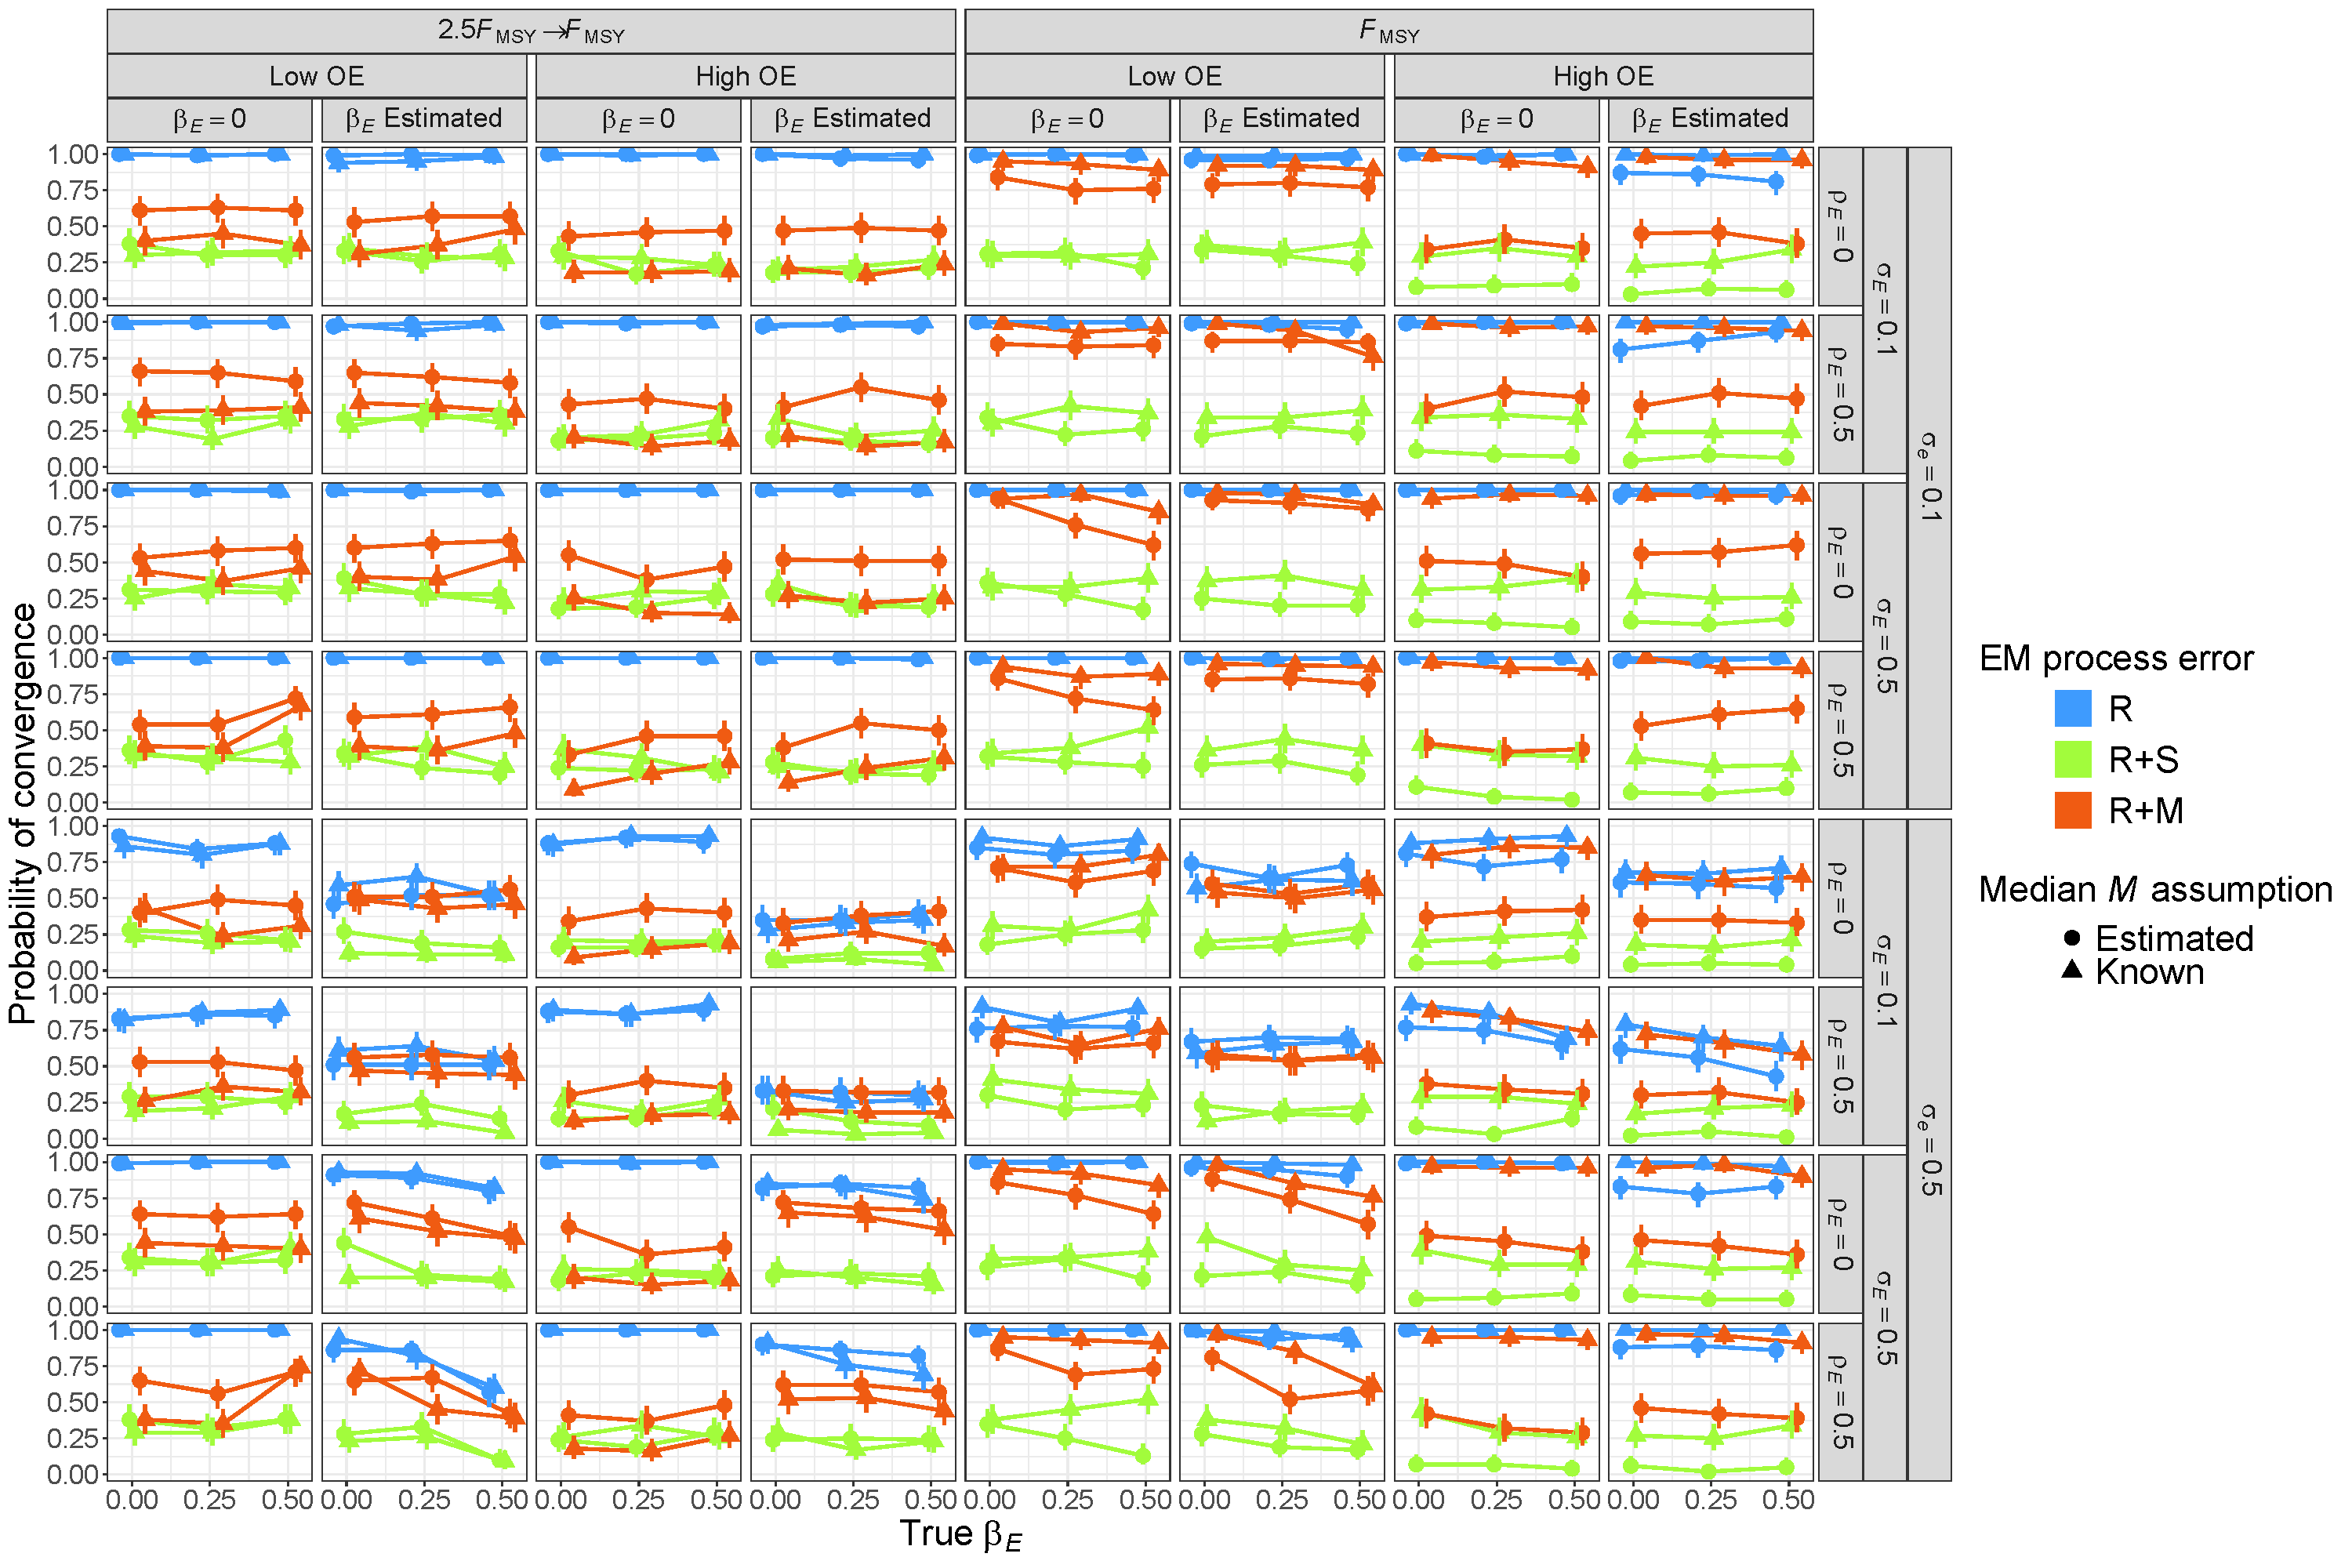
\includegraphics[height = \textheight]{convergence_Rom}
\end{center}
\caption{Estimated probability of fits providing Hessian-based standard errors for estimating models assuming alternative process error, that estimate or assume known median $M$, and that estimate or assume no covariate effect on median $M$ when fitted to R operating models and three levels of true covariate effect on median $M$ (x axis). Vertical lines represent 95\% confidence intervals.}\label{convergence_Rom}
\end{figure}
\end{landscape}

\begin{landscape}
\begin{figure}
\begin{center}
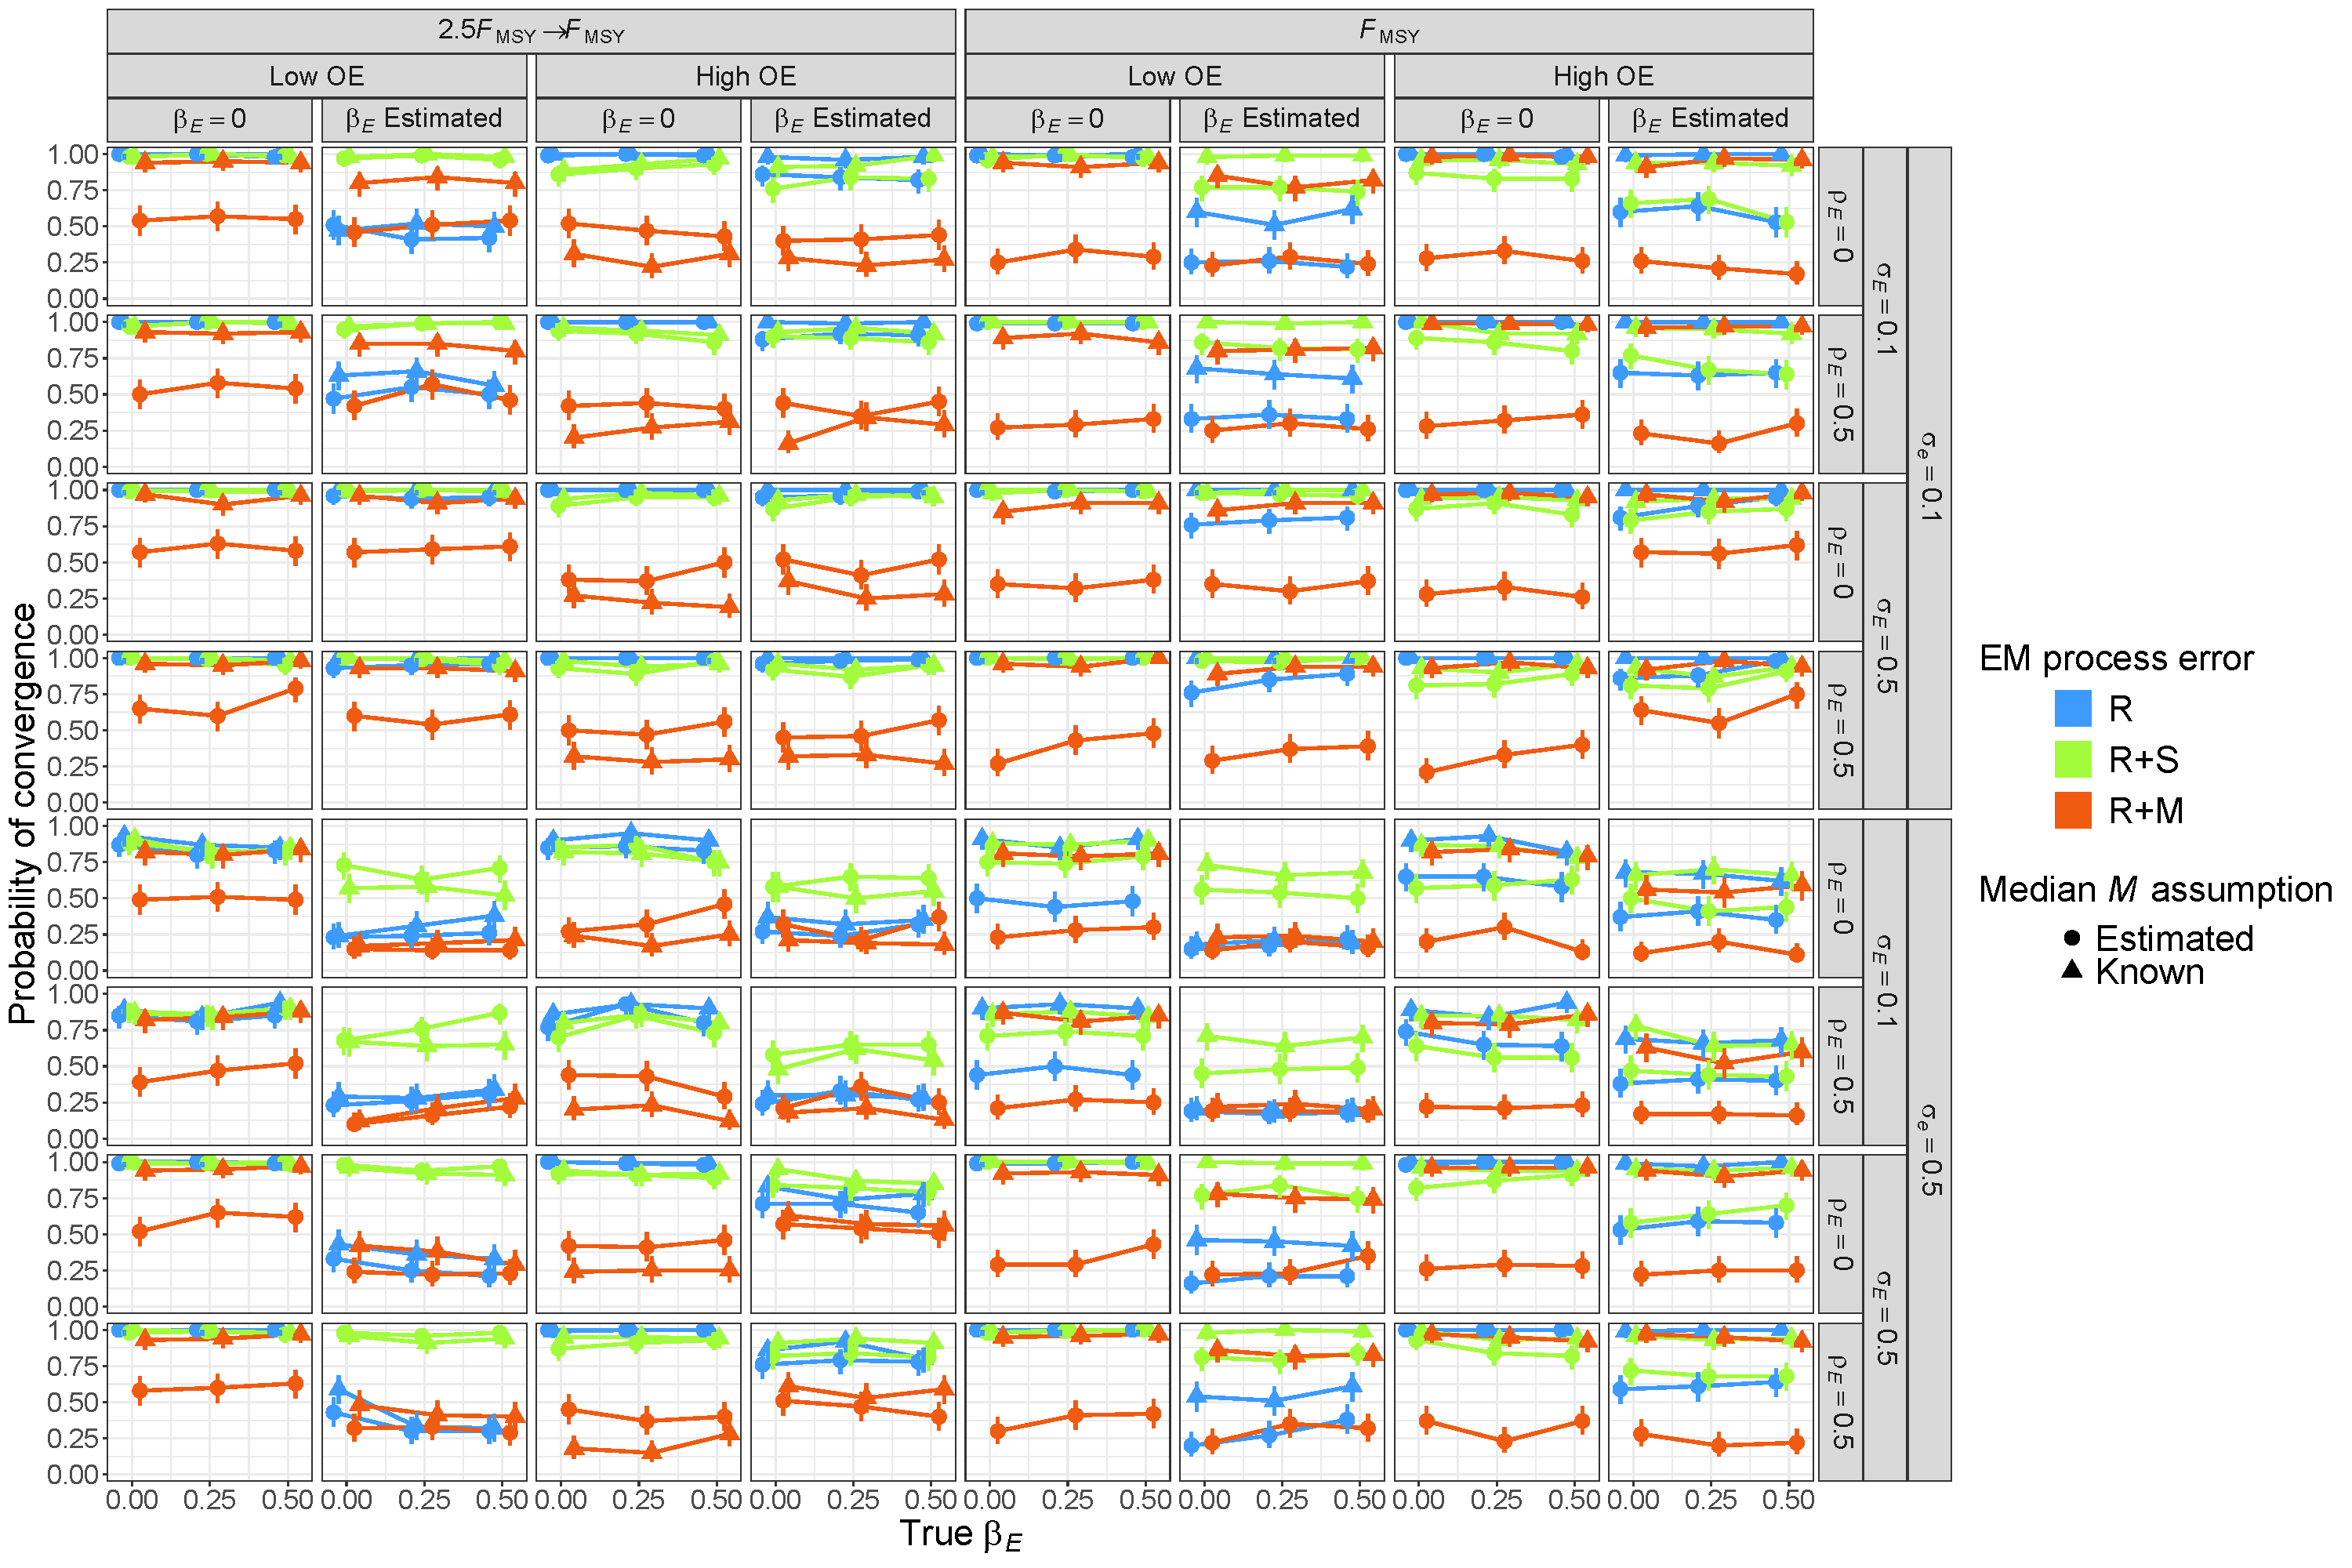
\includegraphics[height = \textheight]{convergence_RSom}
\end{center}
\caption{Estimated probability of fits providing Hessian-based standard errors for estimating models assuming alternative process error, that estimate or assume known median $M$, and that estimate or assume no covariate effect on median $M$ when fitted to R+S operating models and three levels of true covariate effect on median $M$ (x axis). Vertical lines represent 95\% confidence intervals.}\label{convergence_RSom}
\end{figure}
\end{landscape}

\begin{landscape}
\begin{figure}
\begin{center}
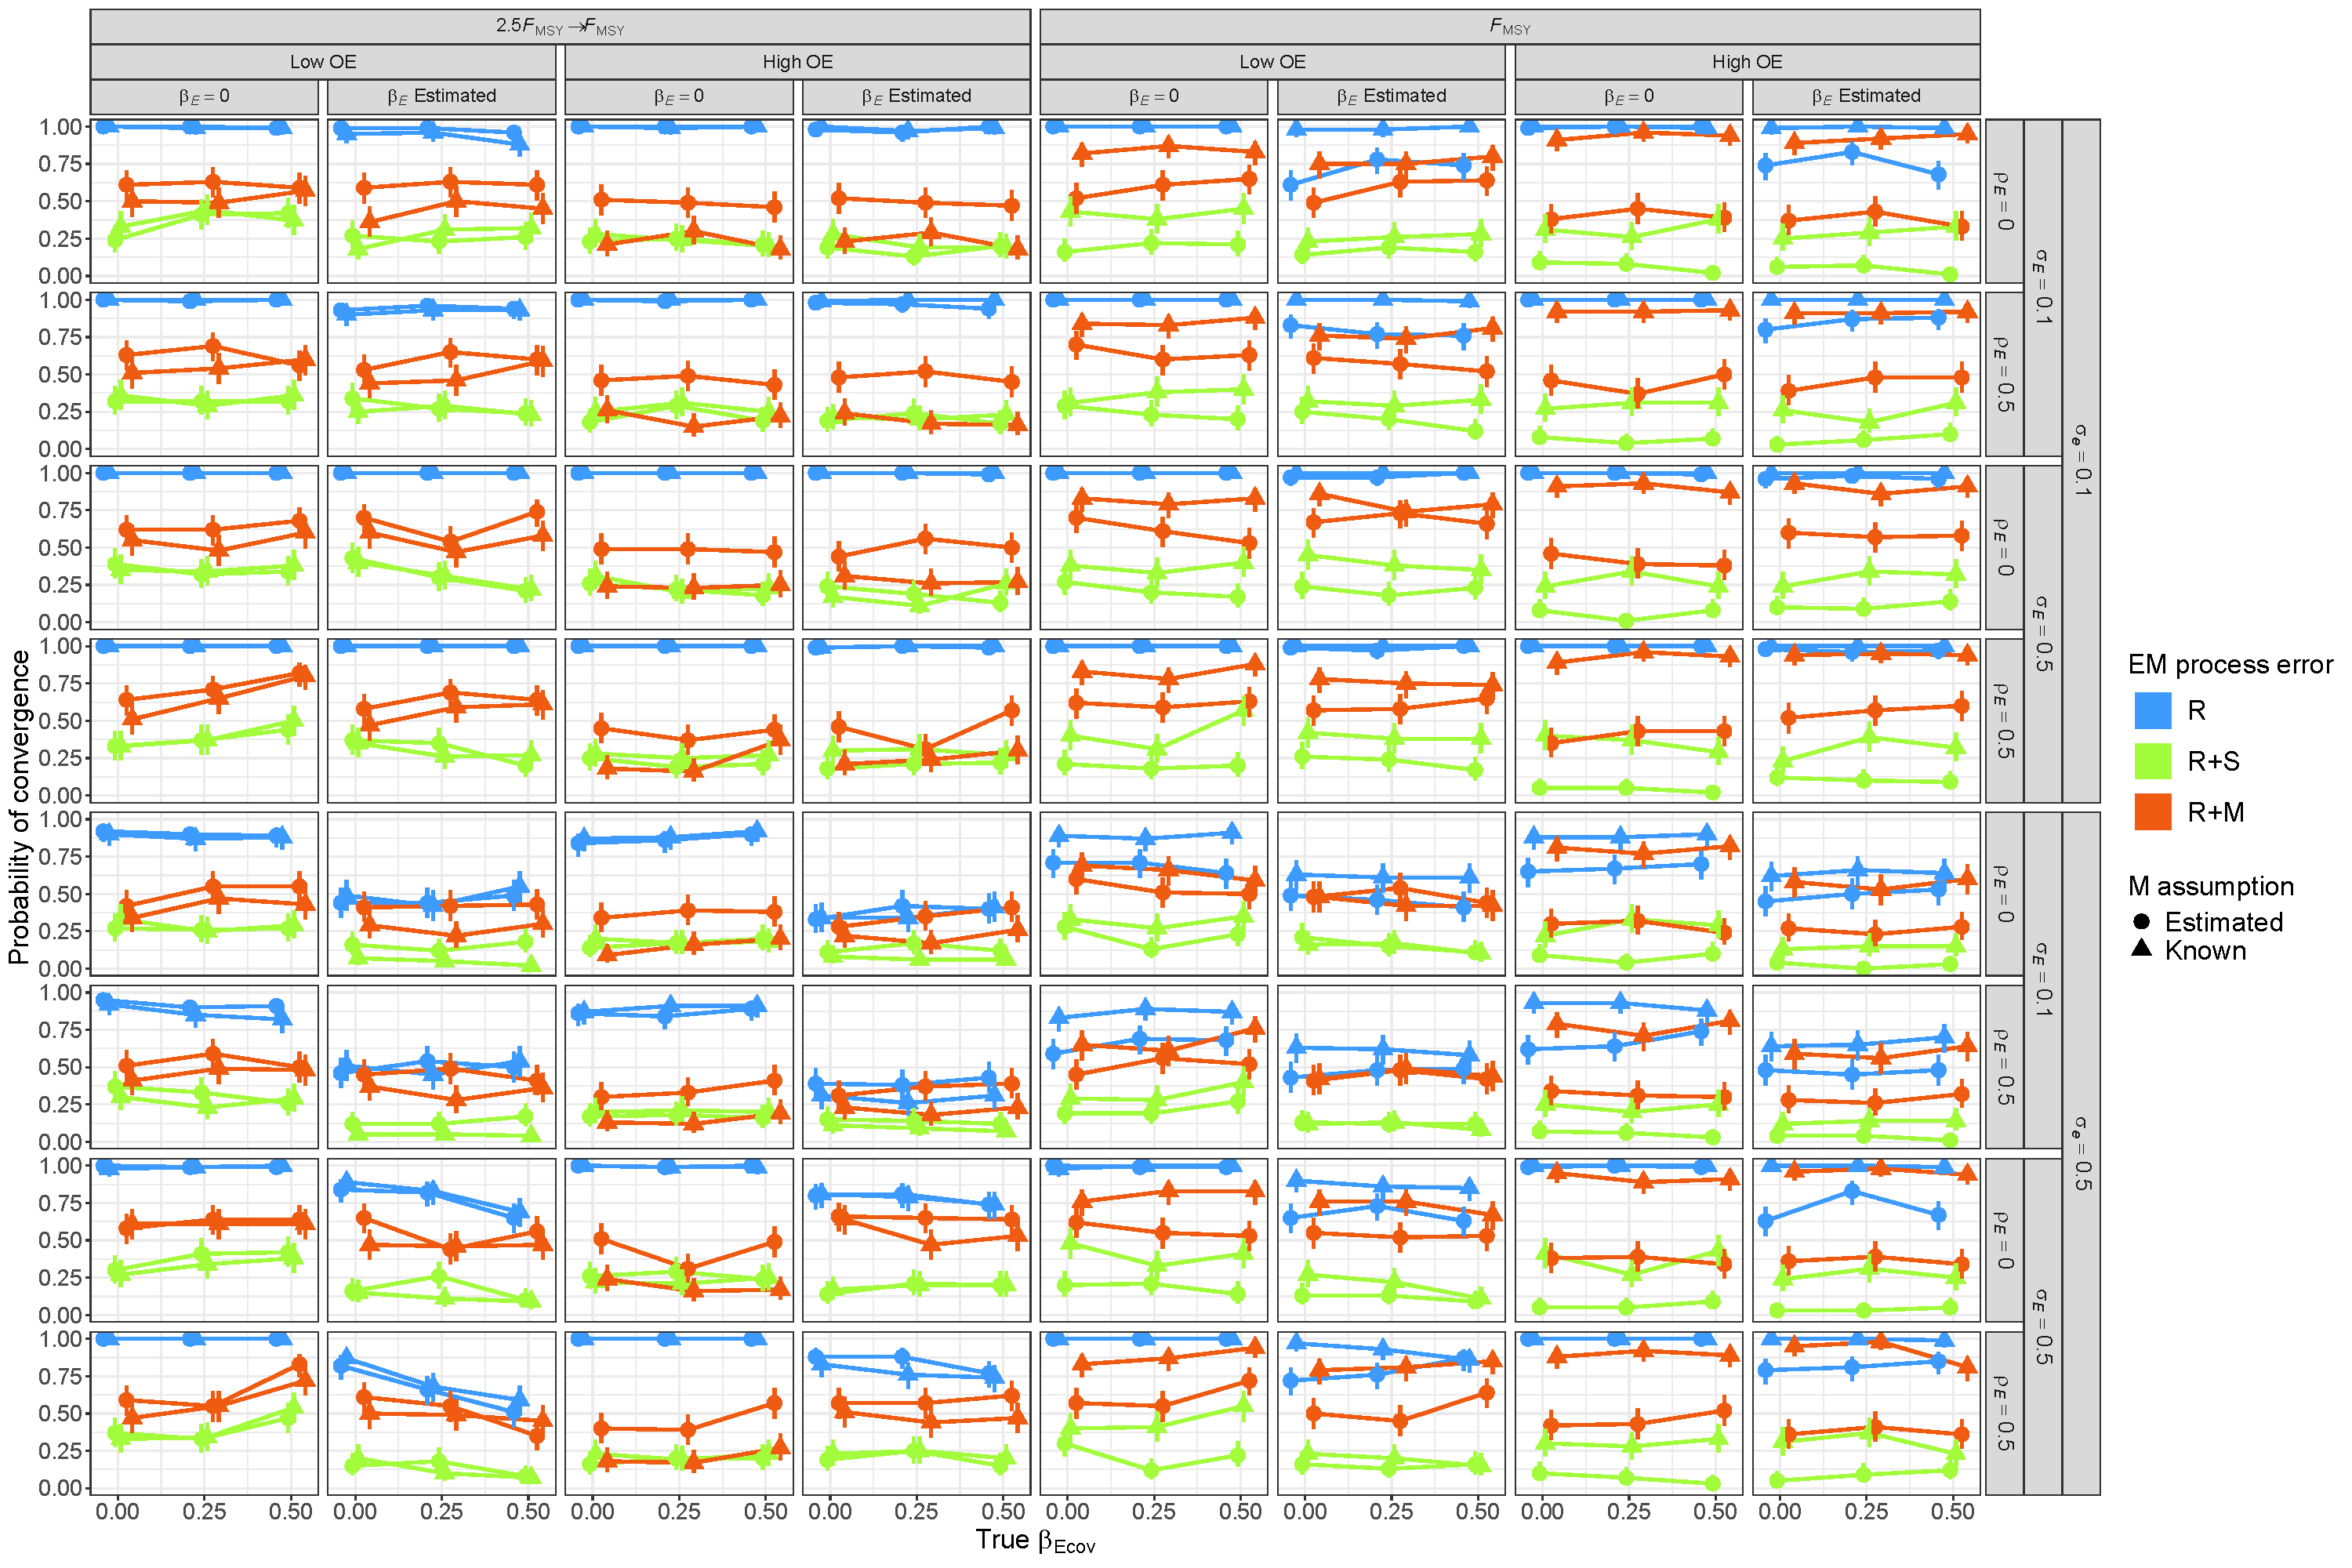
\includegraphics[height = \textheight]{convergence_RMom}
\end{center}
\caption{Estimated probability of fits providing Hessian-based standard errors for estimating models assuming alternative process error, that estimate or assume known median $M$, and that estimate or assume no covariate effect on median $M$ when fitted to R+M operating models and three levels of true covariate effect on median $M$ (x axis). Vertical lines represent 95\% confidence intervals.}\label{convergence_RMom}
\end{figure}
\end{landscape}

\begin{landscape}
\begin{figure}
\begin{center}
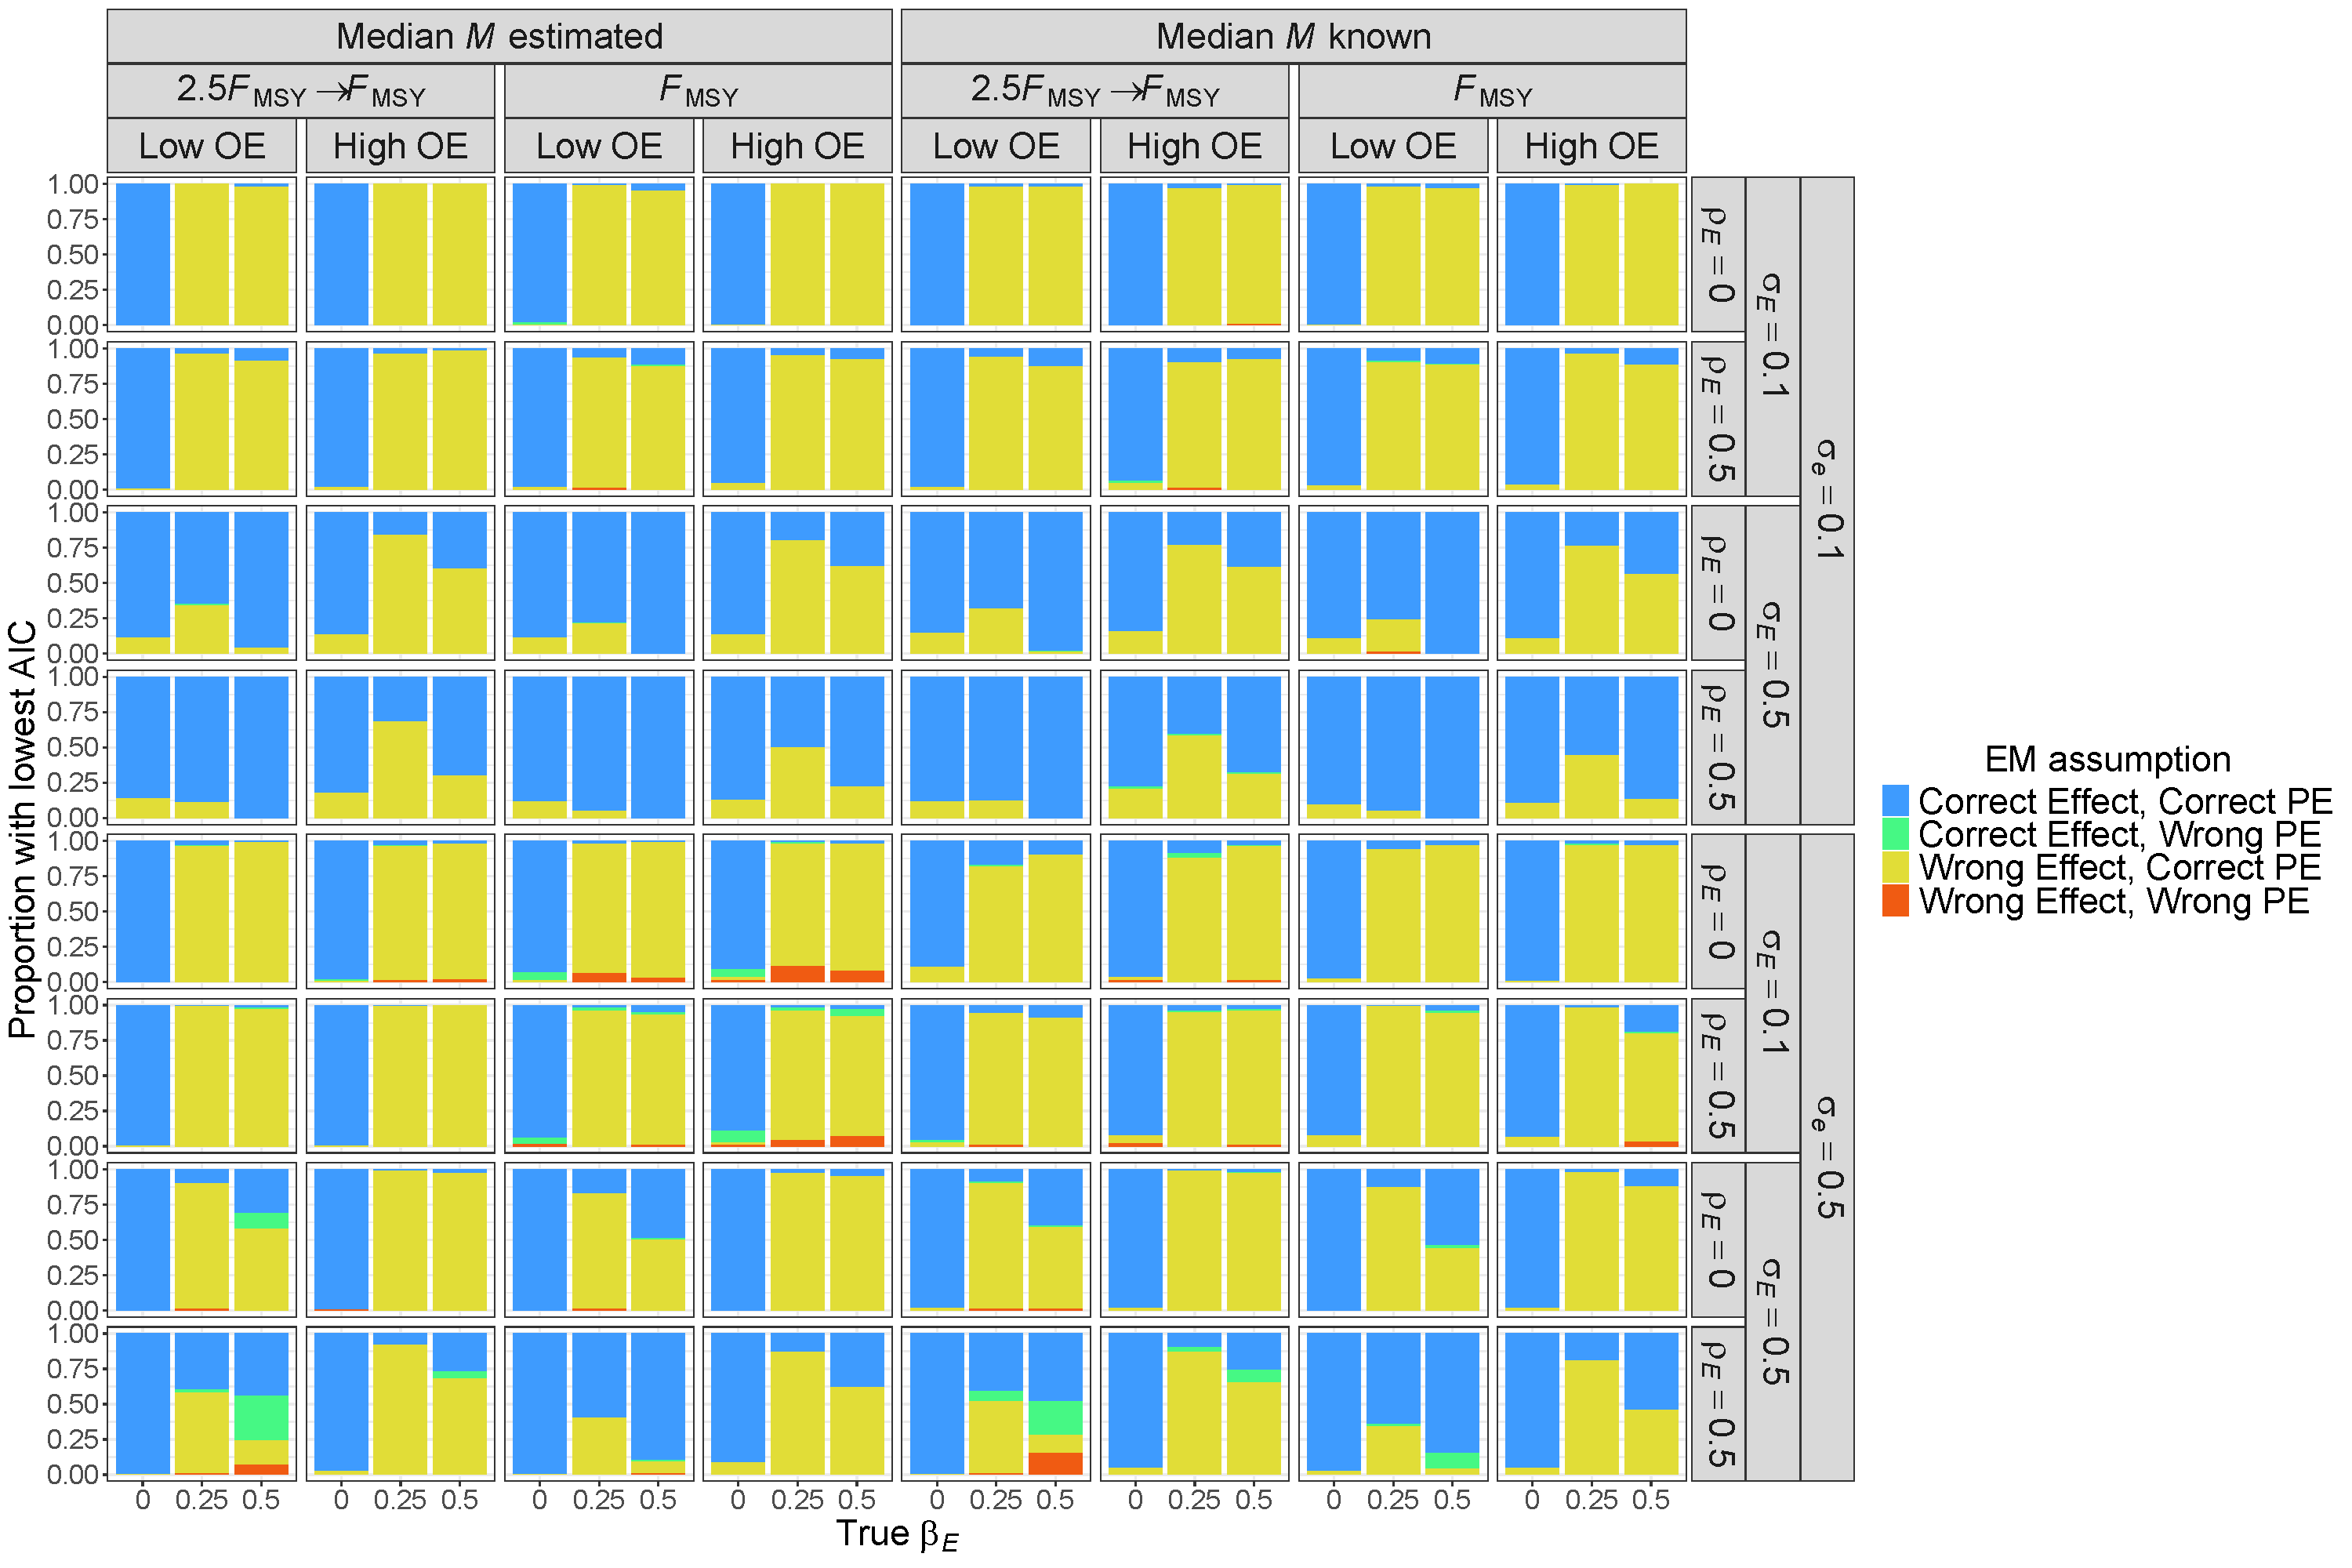
\includegraphics[height = \textheight]{aic_Rom}
\end{center}
\caption{Proportion of simulated data sets for R operating models where the estimating model type (treatment of environmental covariate and assumed process error type) had the lowest AIC.}\label{aic_Rom}
\end{figure}
\end{landscape}

\begin{landscape}
\begin{figure}
\begin{center}
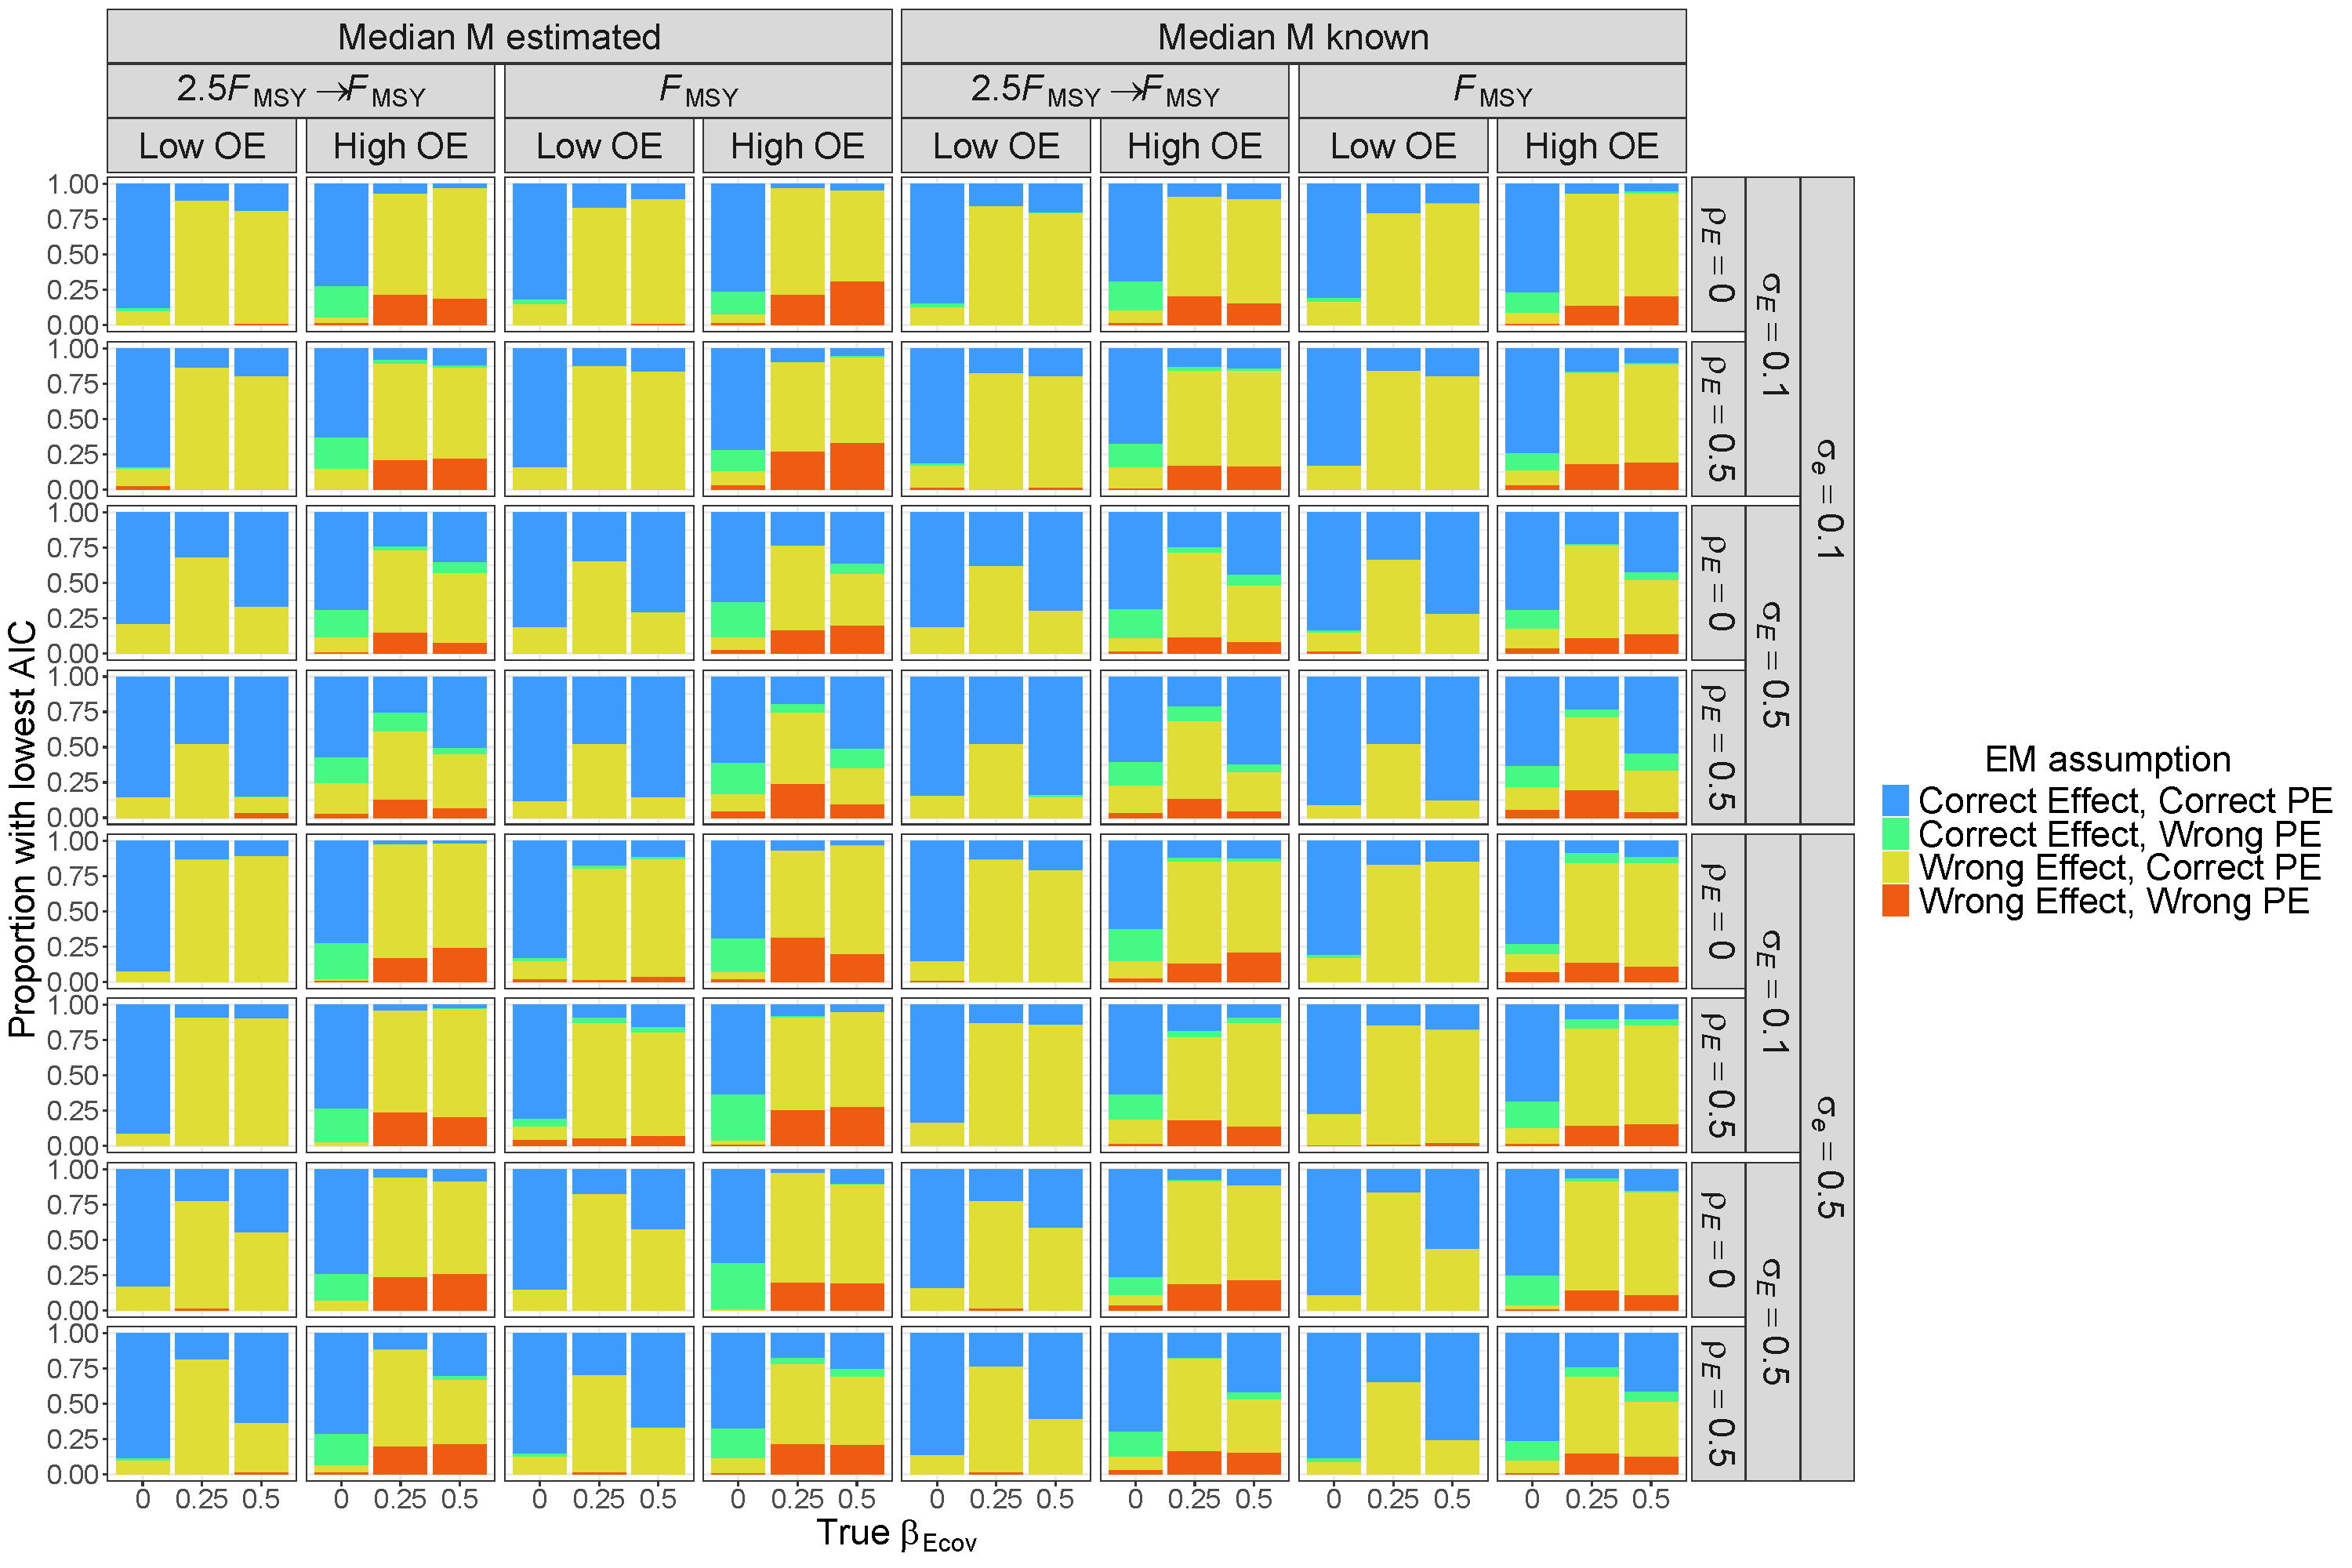
\includegraphics[height = \textheight]{aic_RSom}
\end{center}
\caption{Proportion of simulated data sets for R+S operating models where the estimating model type (treatment of environmental covariate and assumed process error type) had the lowest AIC.}\label{aic_RSom}
\end{figure}
\end{landscape}

\begin{landscape}
\begin{figure}
\begin{center}
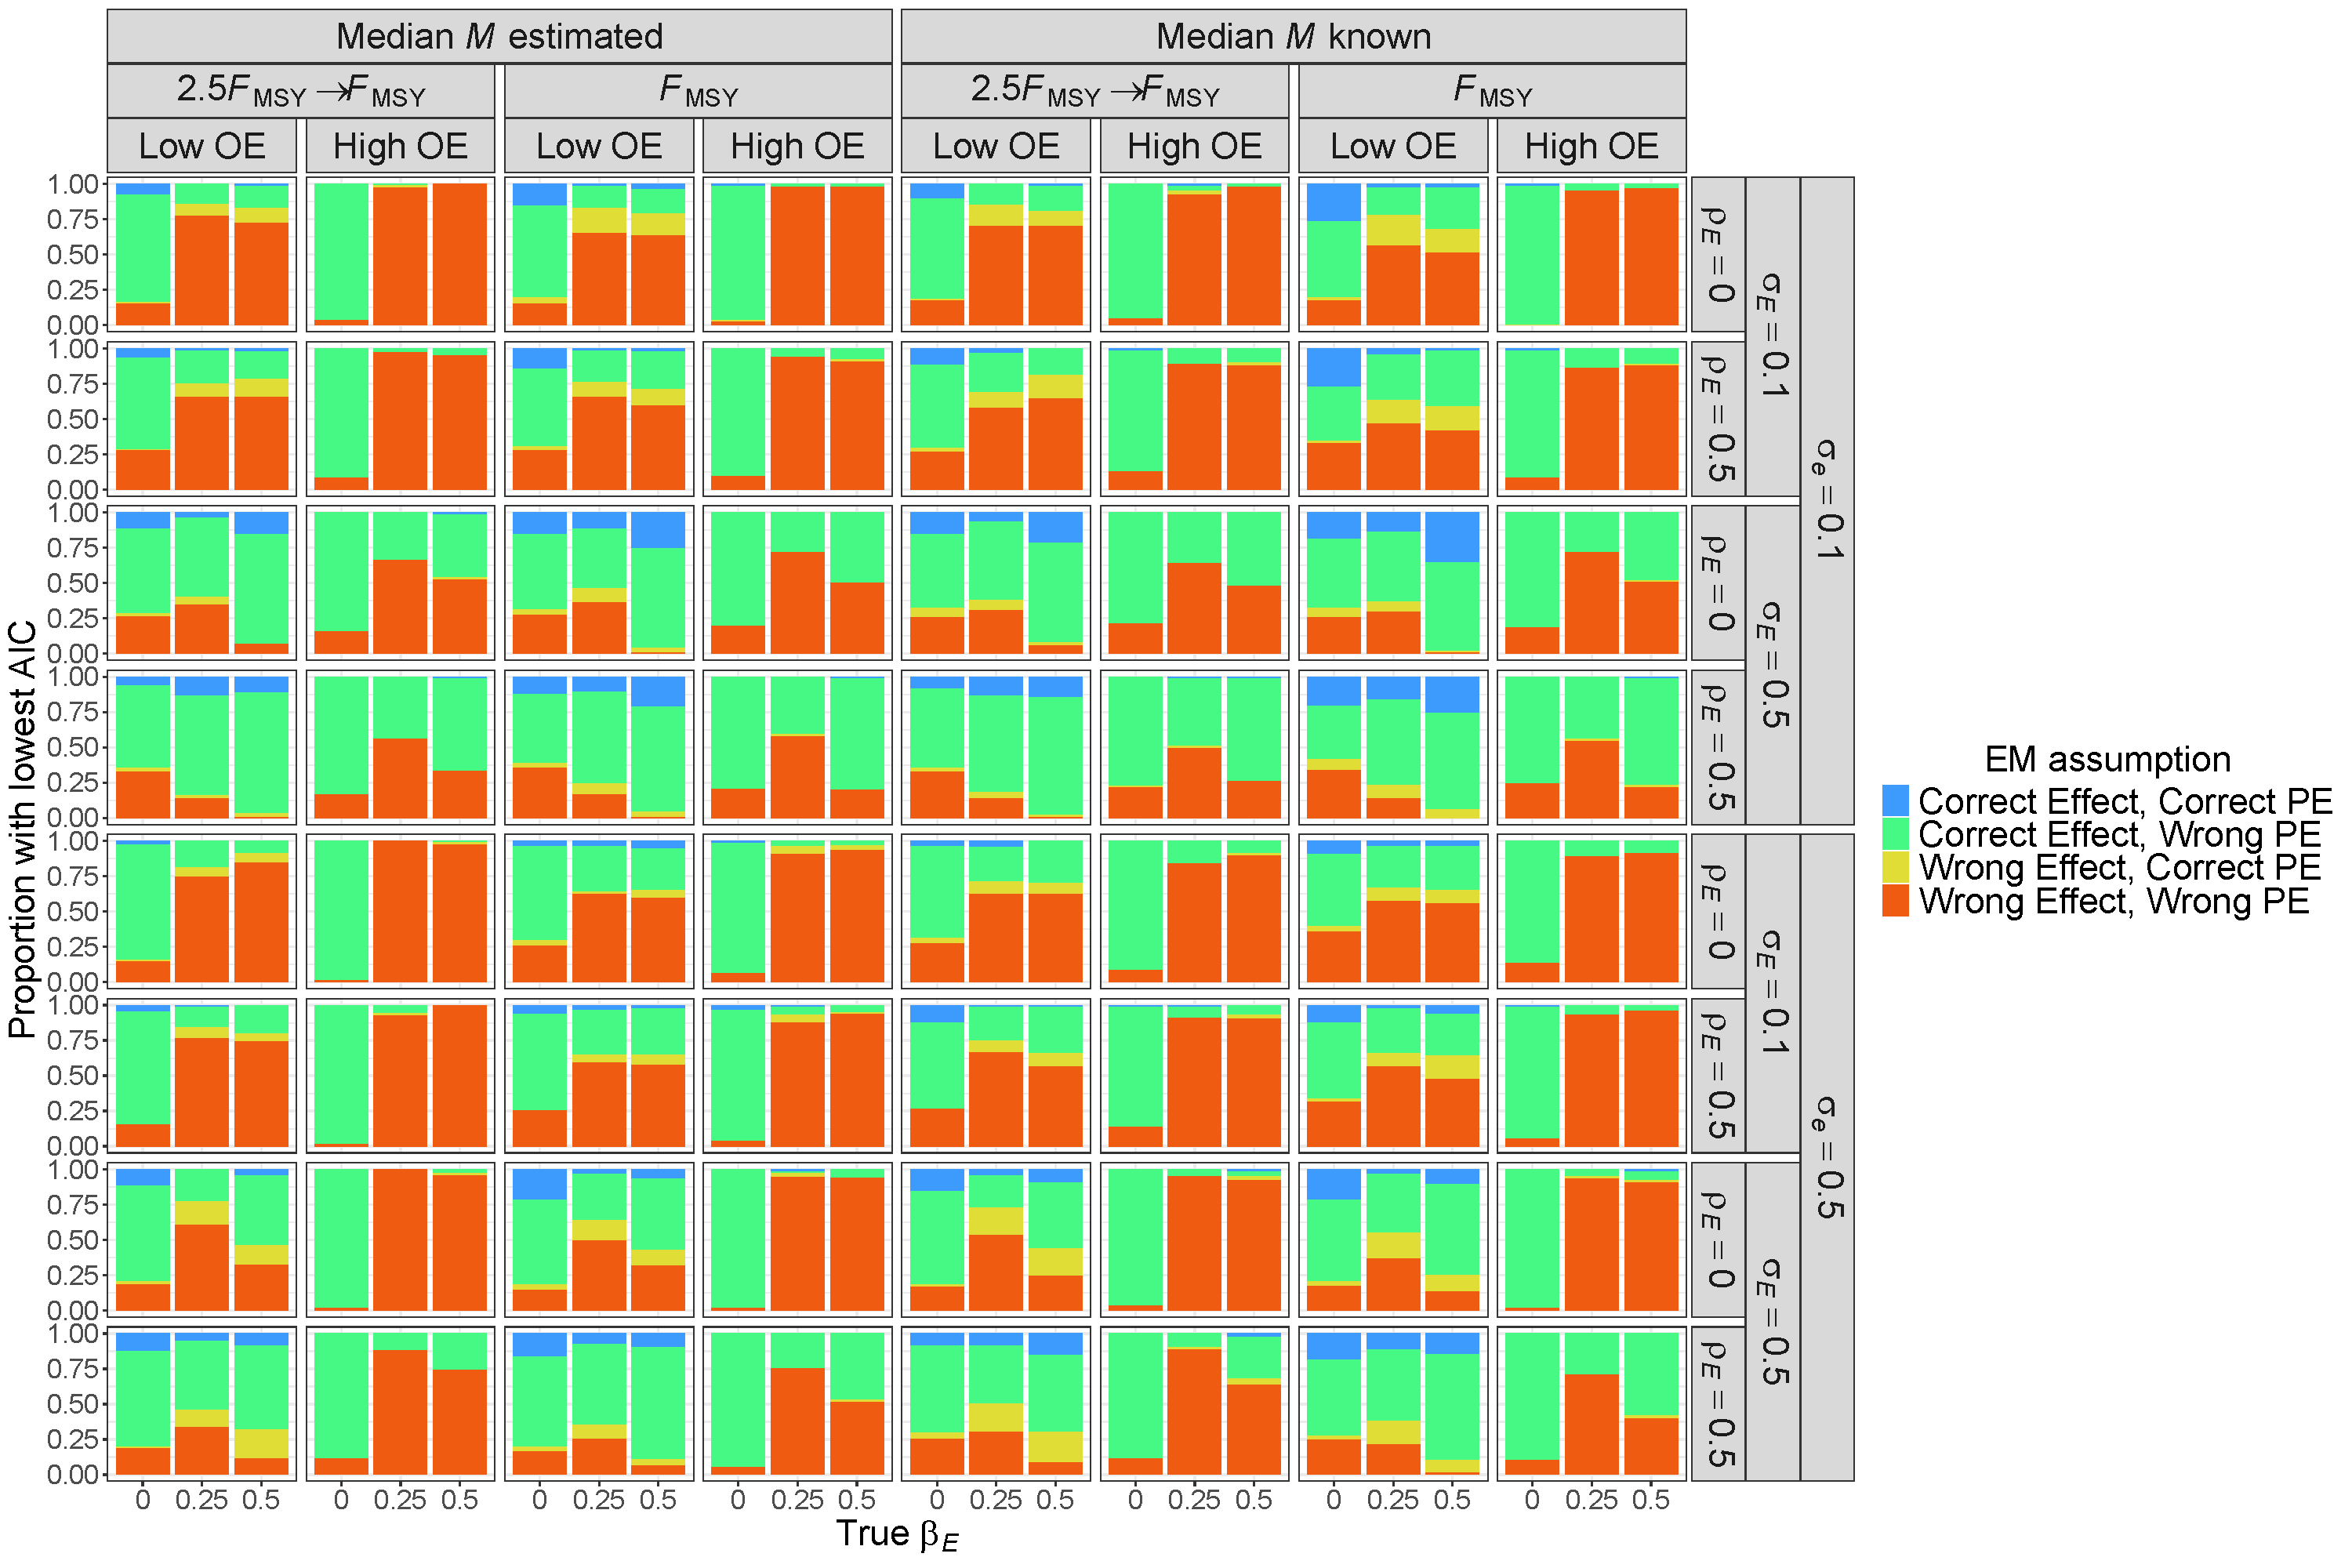
\includegraphics[height = \textheight]{aic_RMom}
\end{center}
\caption{Proportion of simulated data sets for R+M operating models where the estimating model type (treatment of environmental covariate and assumed process error type) had the lowest AIC.}\label{aic_RMom}
\end{figure}
\end{landscape}

\begin{landscape}
\begin{figure}
\begin{center}
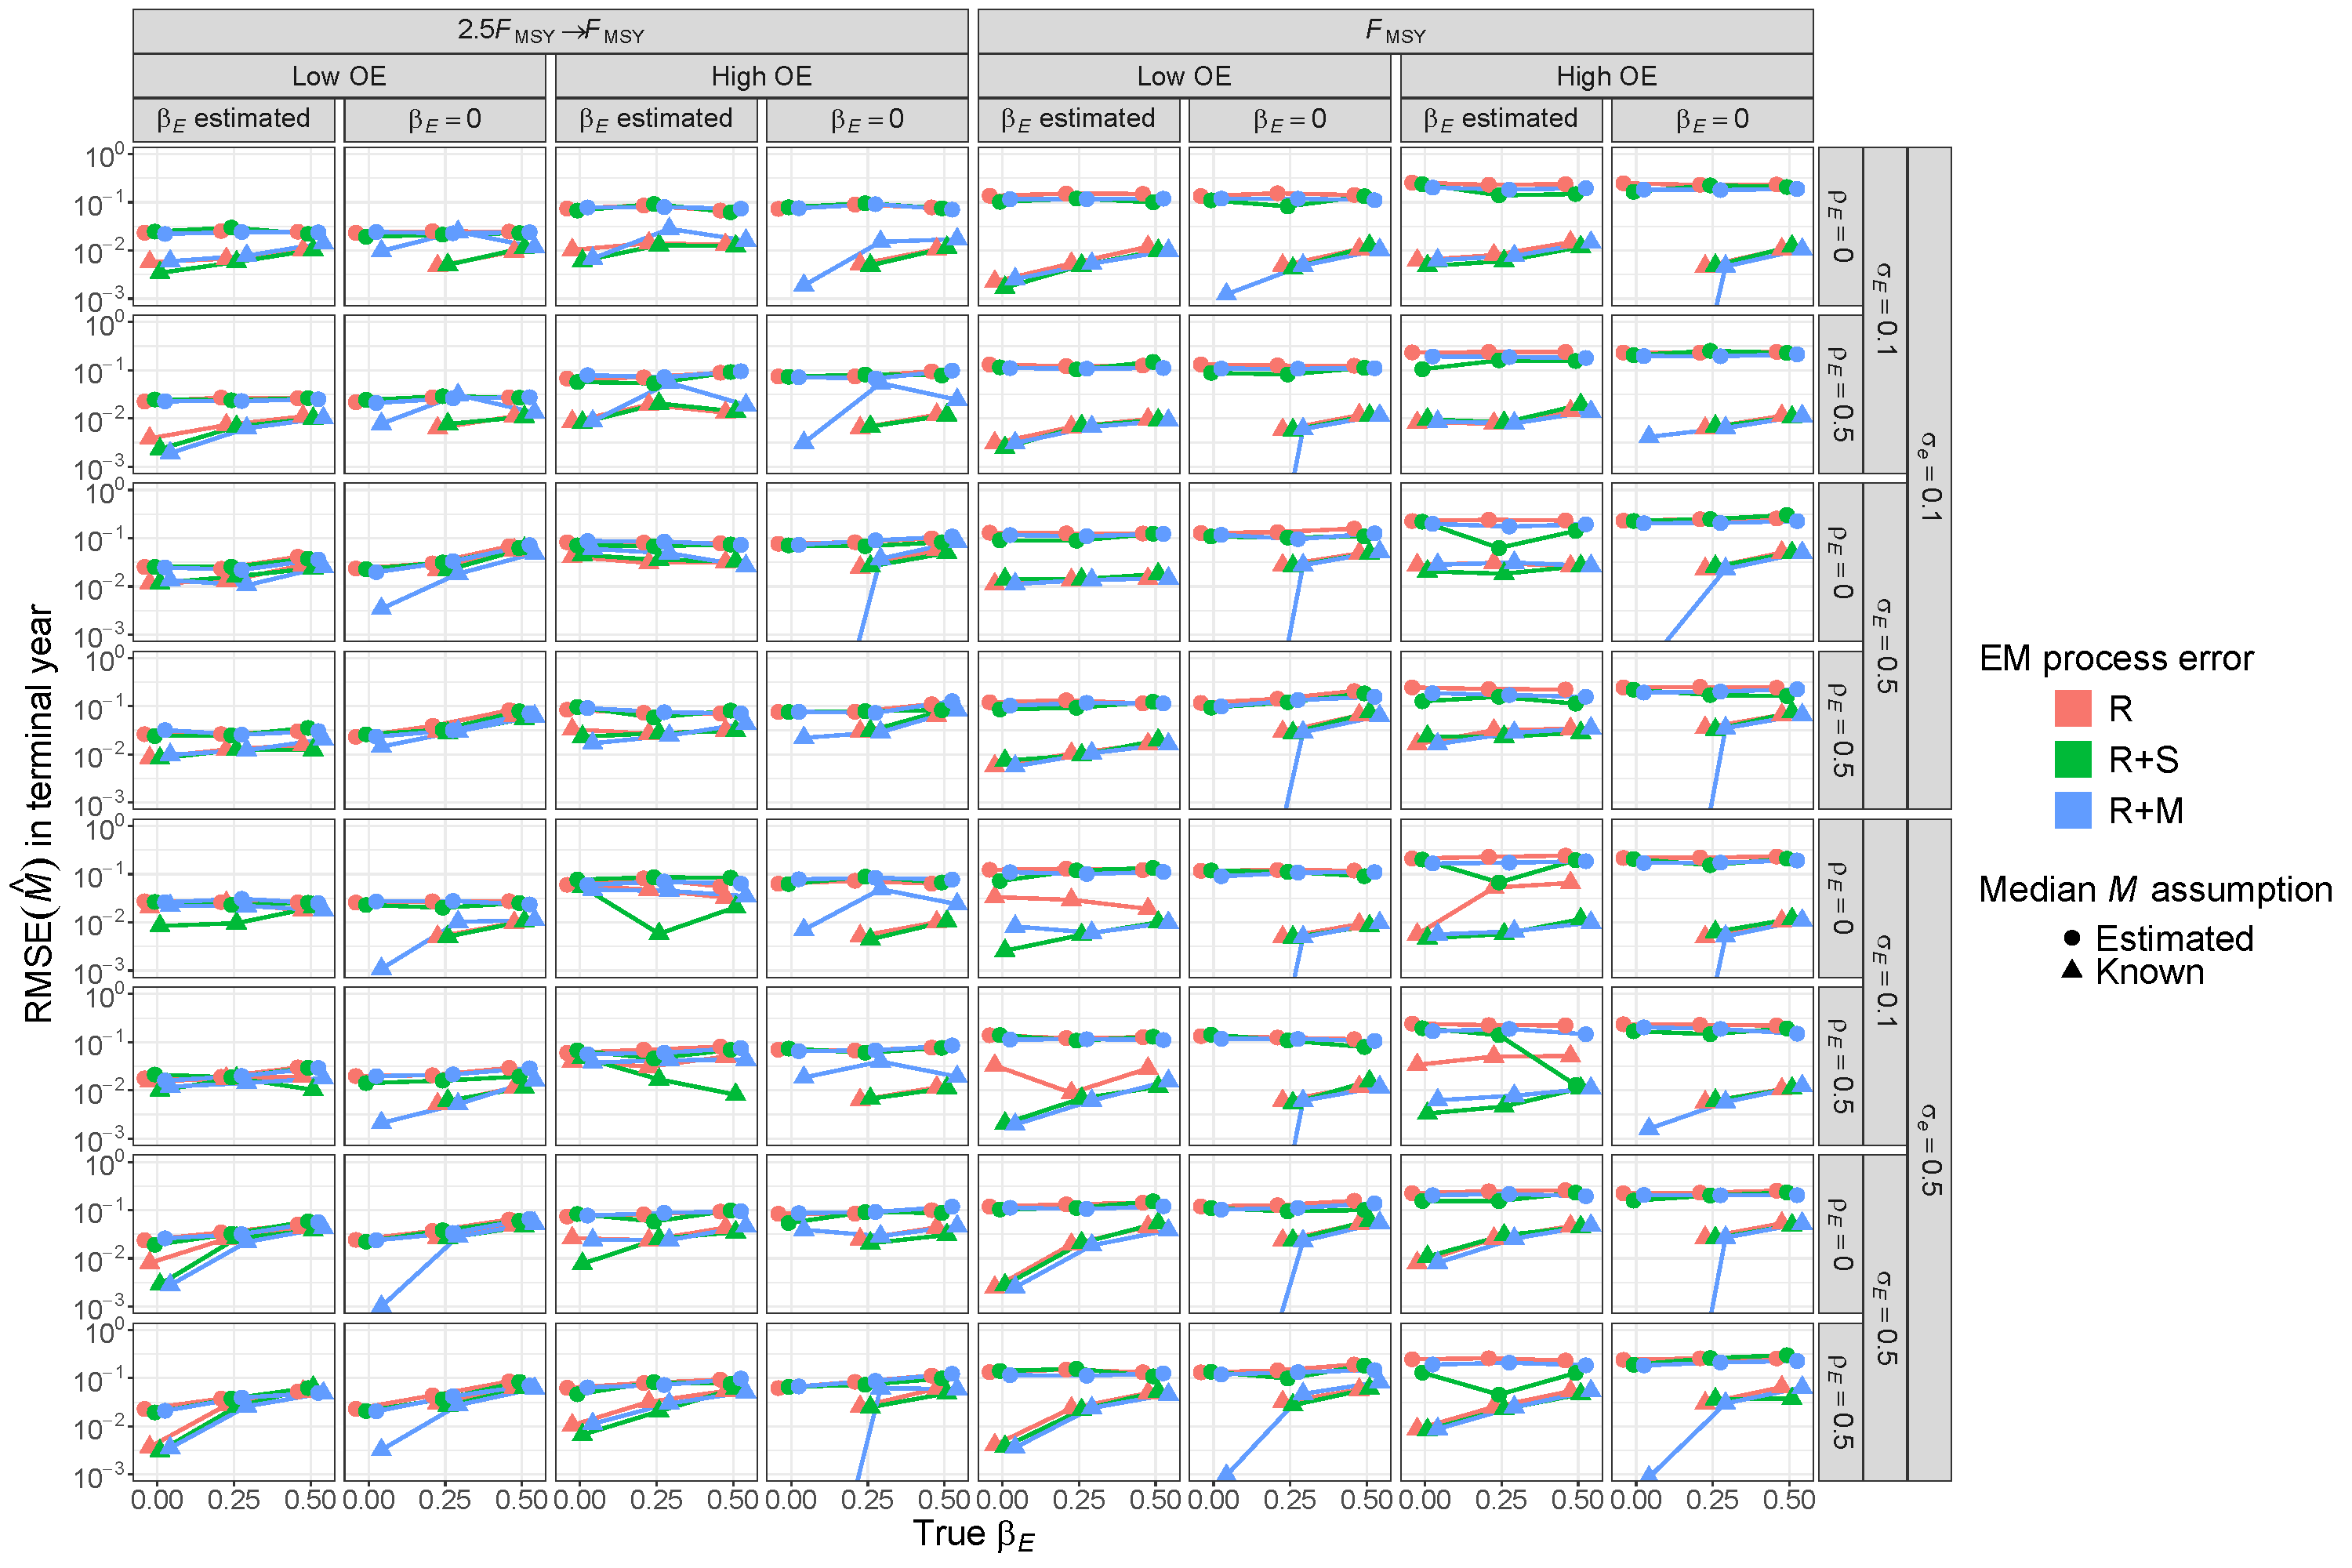
\includegraphics[height = \textheight]{terminal_year_M_rmse_Rom}
\end{center}
\caption{For R operating models, RMSE of estimates of terminal year $M$ for estimating models with alternative process error assumptions, treatment of covariate effect ($\beta_E = 0$ or estimated), and treatment of median $M$ parameter ($\beta_M$ estimated or known).}\label{terminal_M_rmse_Rom}
\end{figure}
\end{landscape}

\begin{landscape}
\begin{figure}
\begin{center}
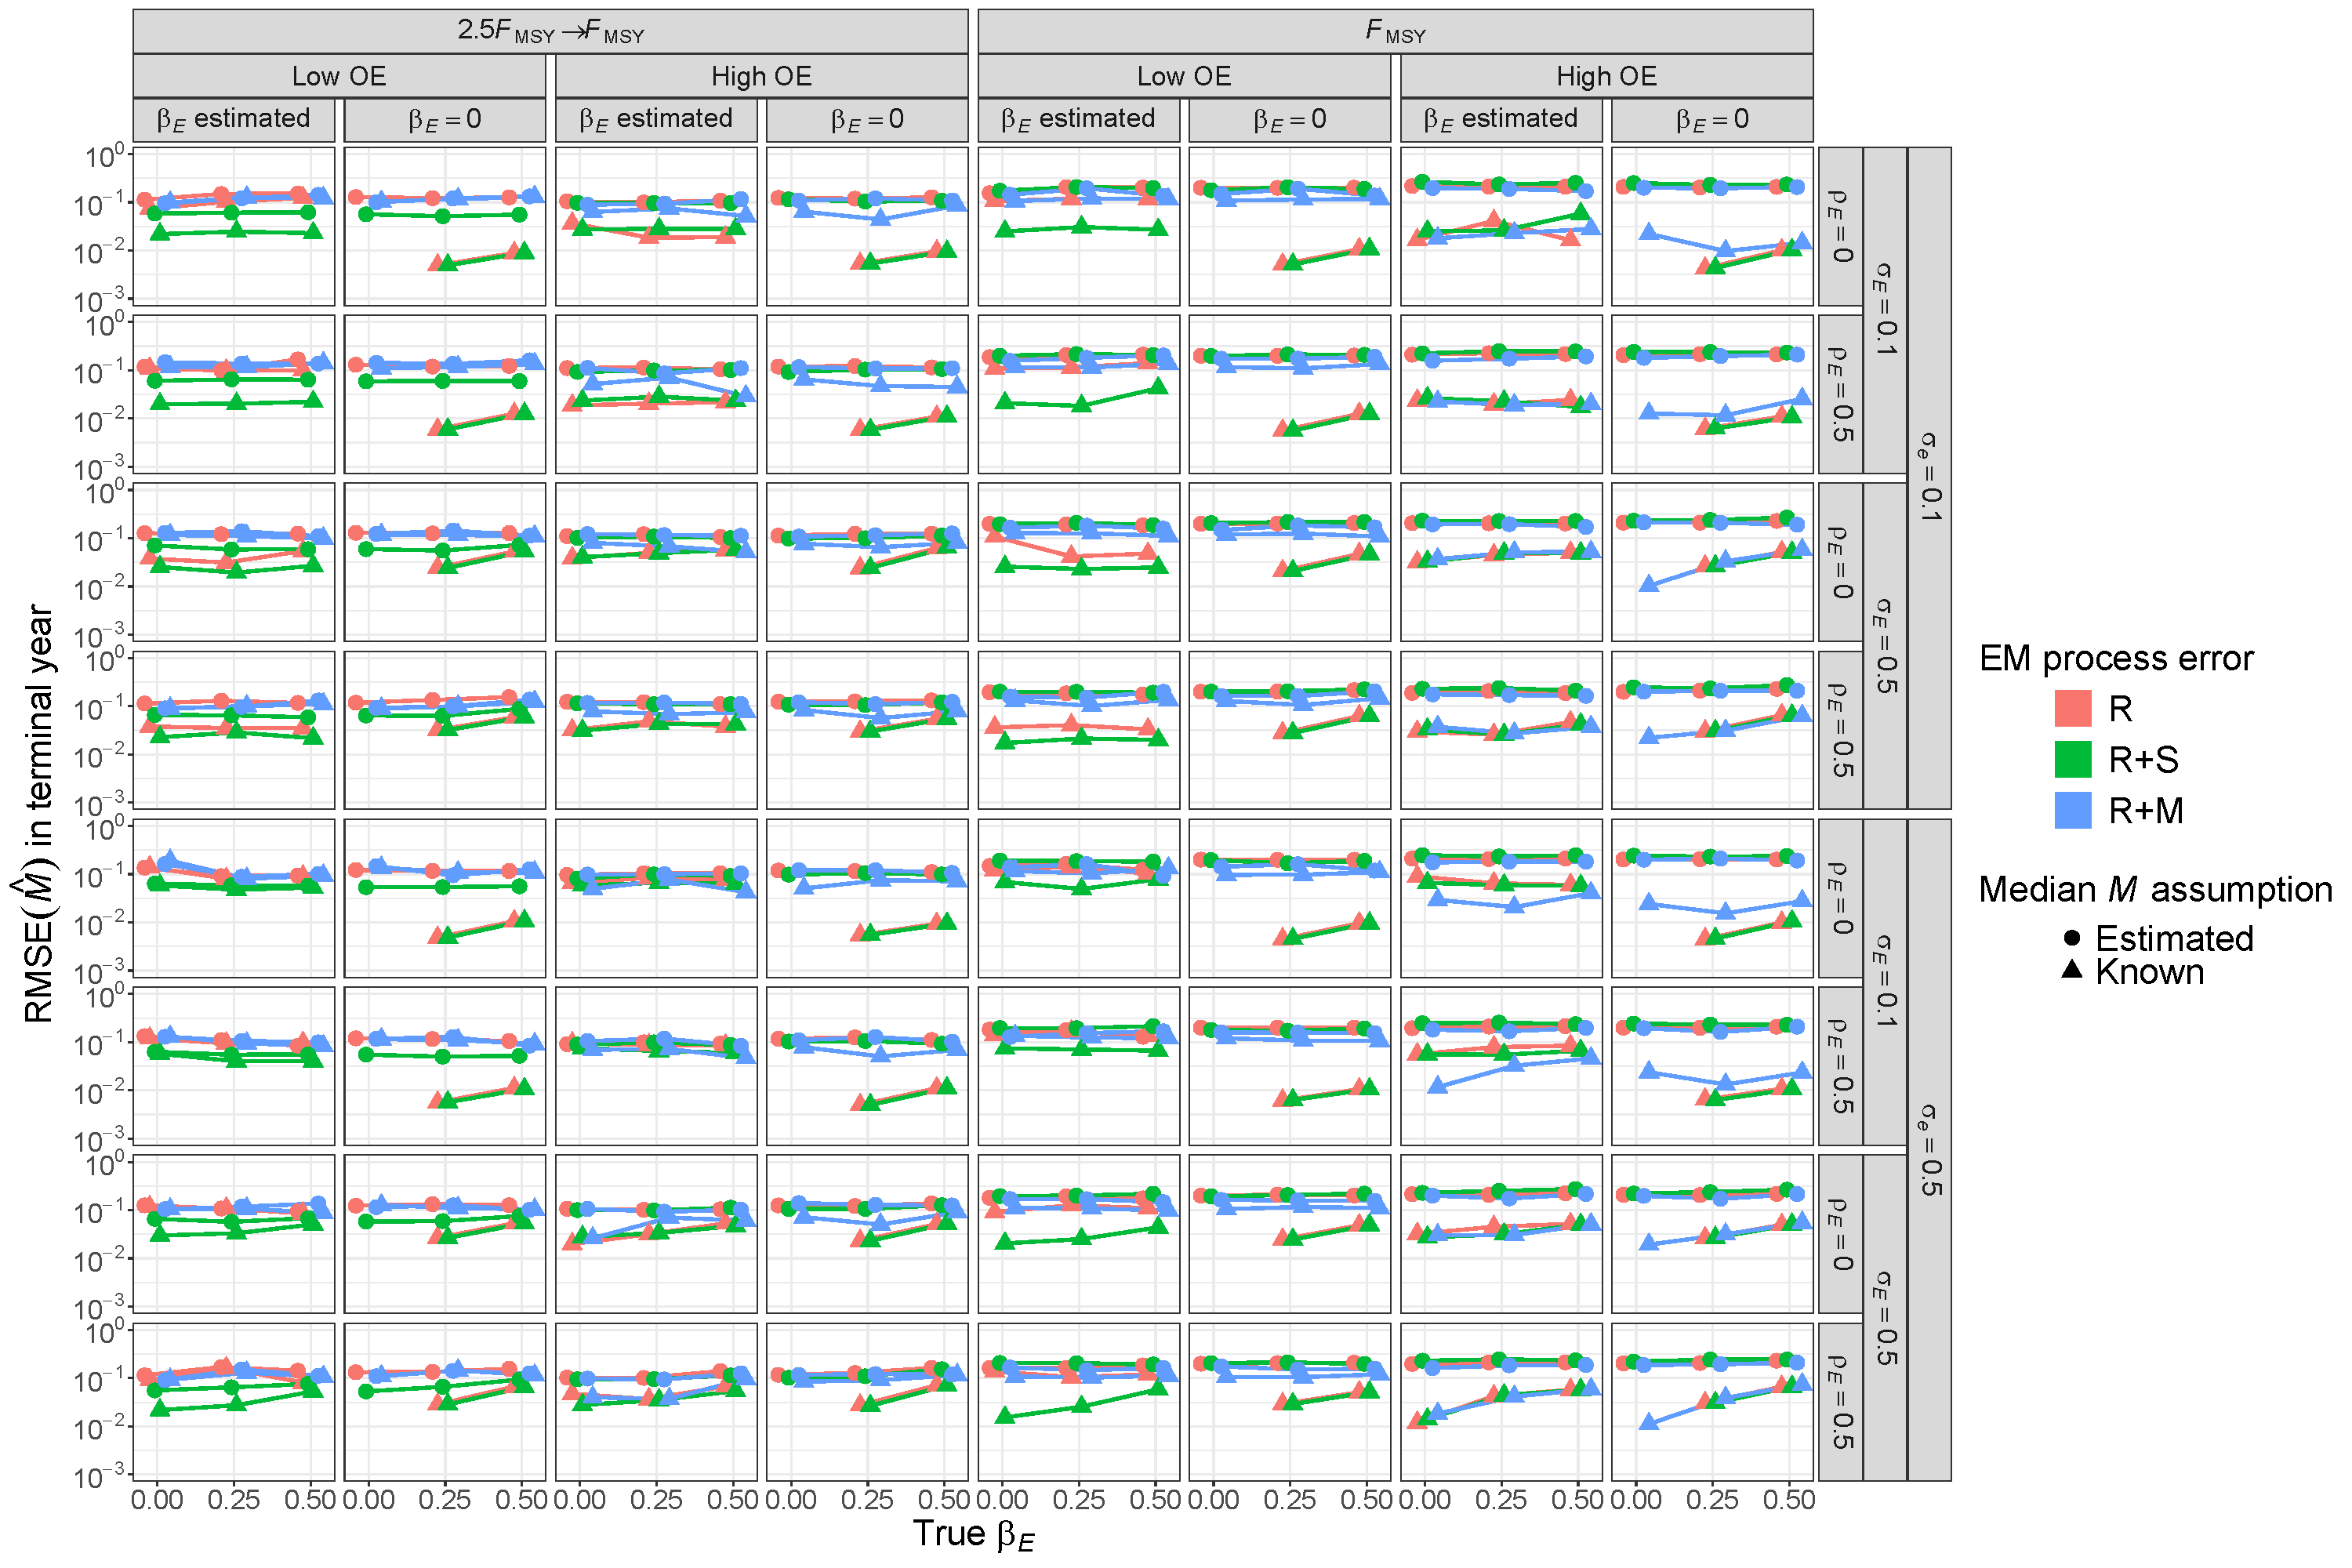
\includegraphics[height = \textheight]{terminal_year_M_rmse_RSom}
\end{center}
\caption{For R+S operating models, RMSE of estimates of terminal year $M$ for estimating models with alternative process error assumptions, treatment of covariate effect ($\beta_E = 0$ or estimated), and treatment of median $M$ parameter ($\beta_M$ estimated or known).}\label{terminal_M_rmse_RSom}
\end{figure}
\end{landscape}

\begin{landscape}
\begin{figure}
\begin{center}
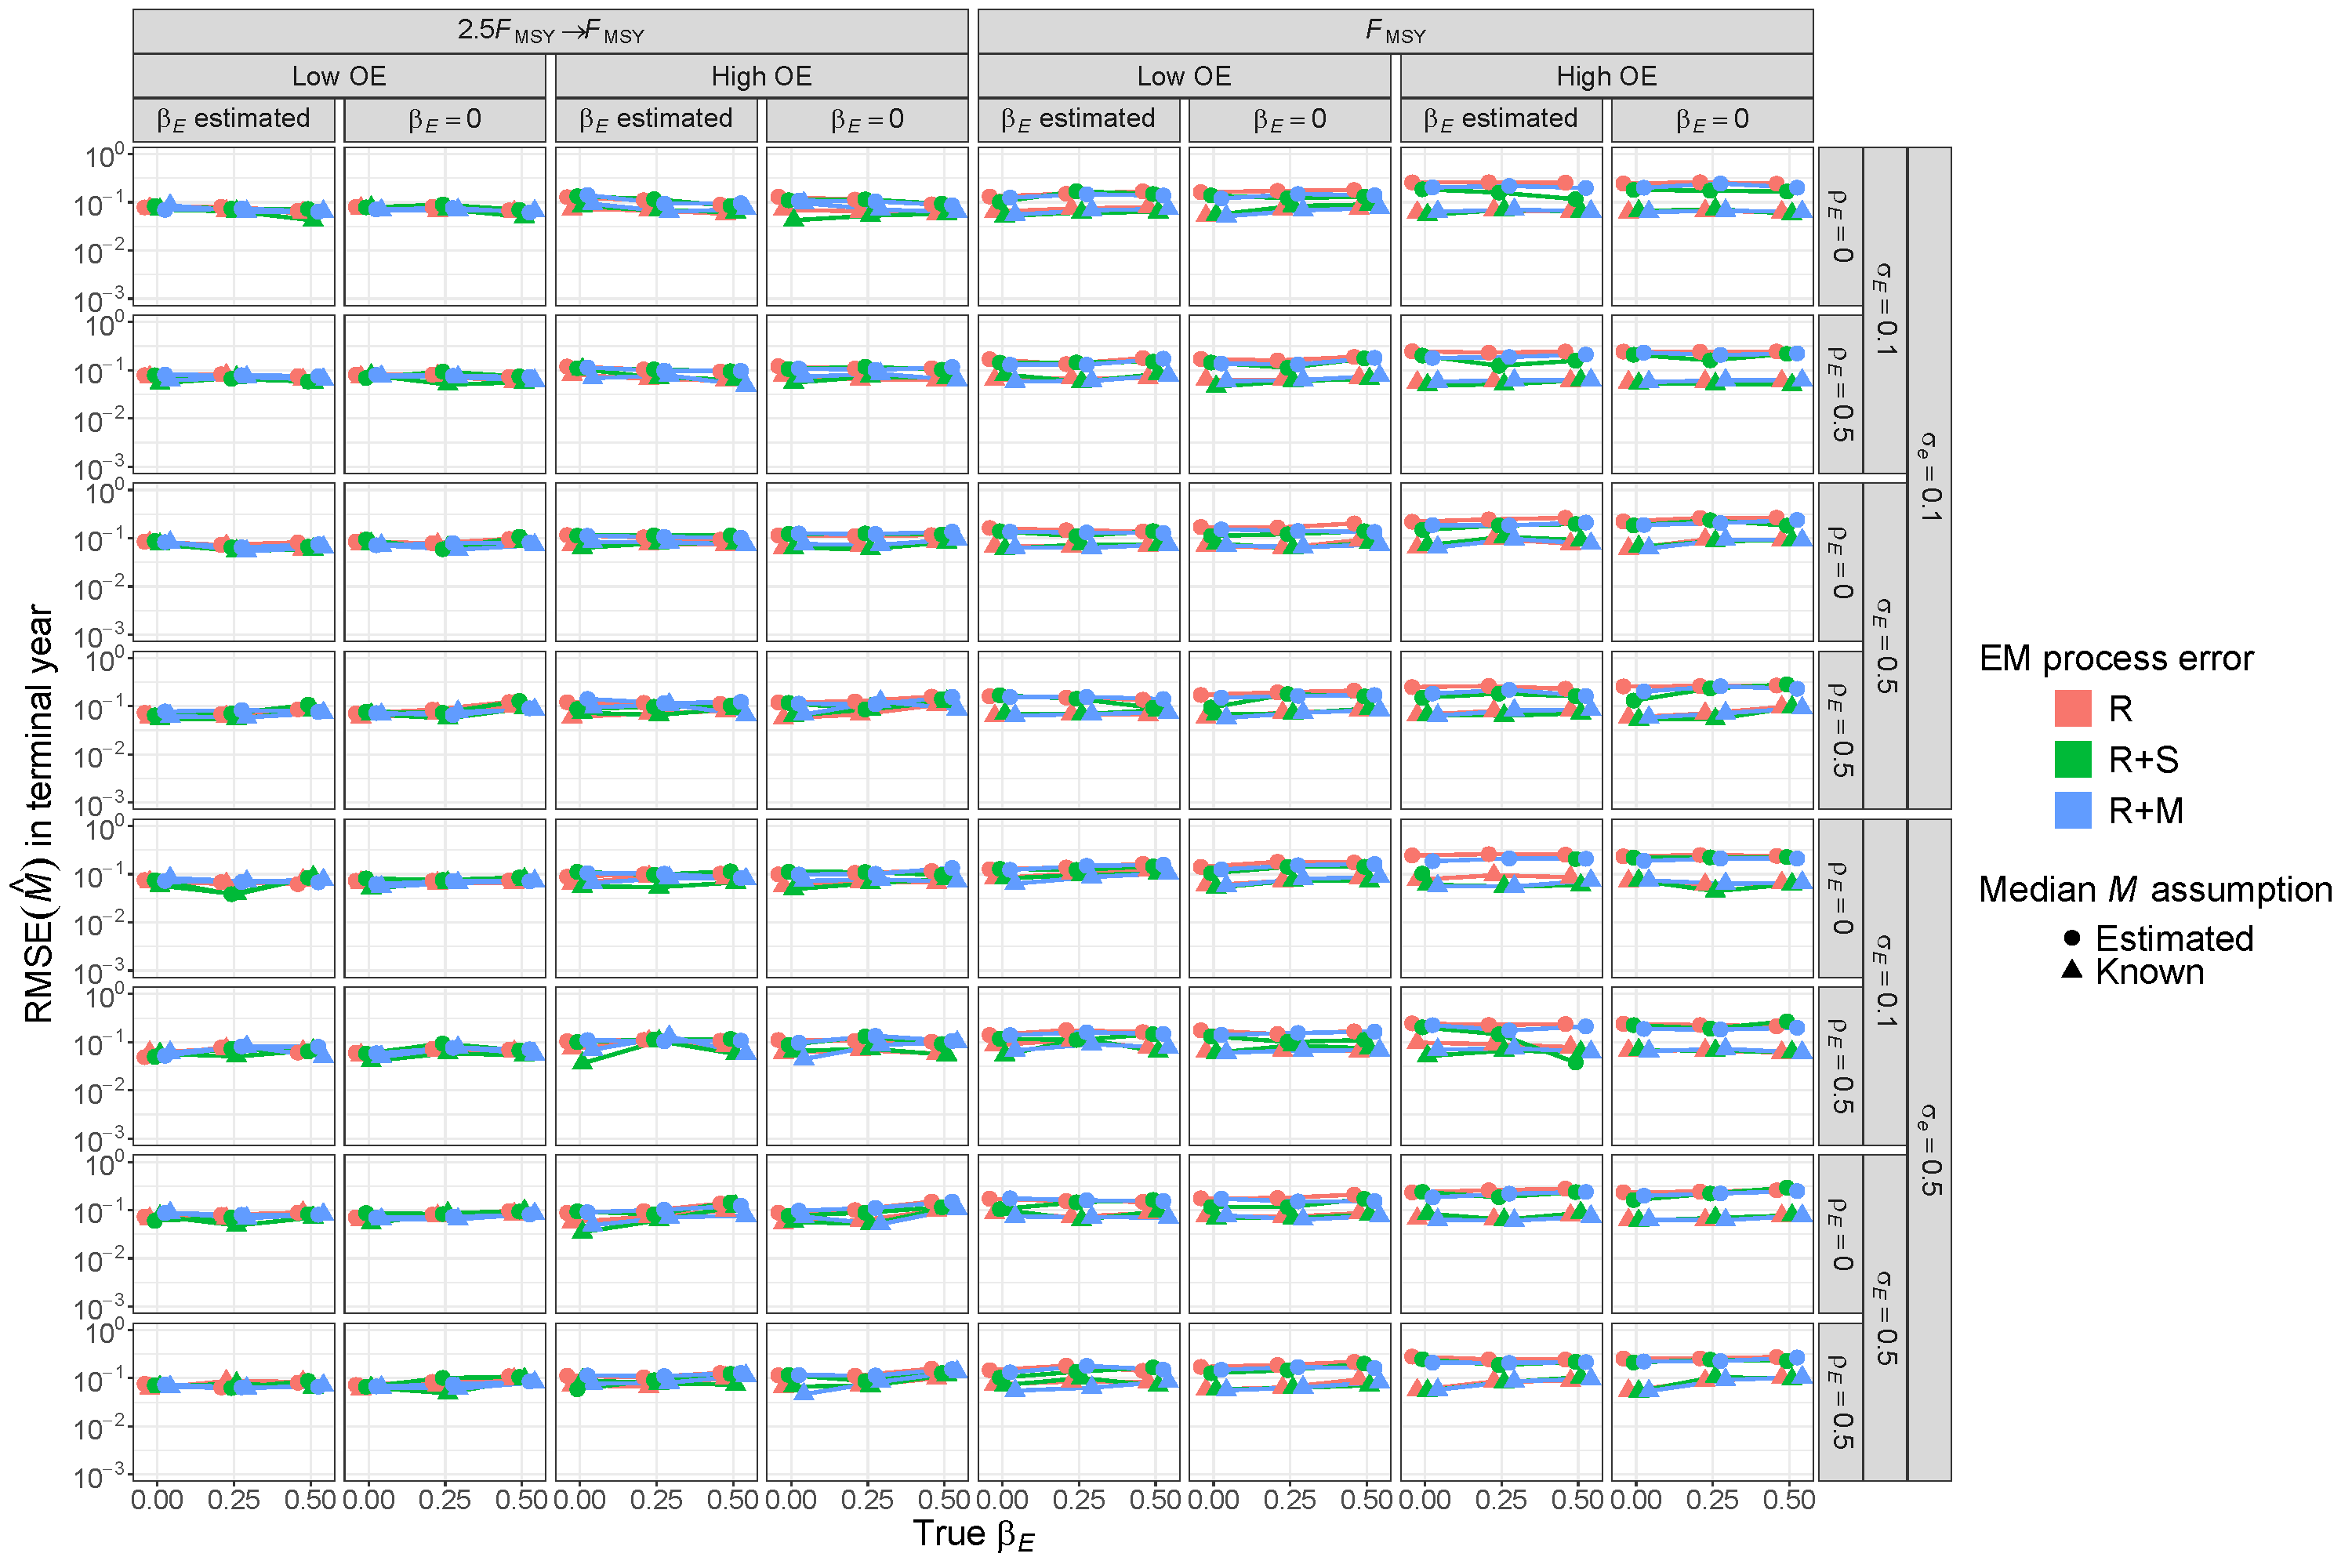
\includegraphics[height = \textheight]{terminal_year_M_rmse_RMom}
\end{center}
\caption{For R+M operating models, RMSE of estimates of terminal year $M$ for estimating models with alternative process error assumptions, treatment of covariate effect ($\beta_E = 0$ or estimated), and treatment of median $M$ parameter ($\beta_M$ estimated or known).}\label{terminal_M_rmse_RMom}
\end{figure}
\end{landscape}

\begin{landscape}
\begin{figure}
\begin{center}
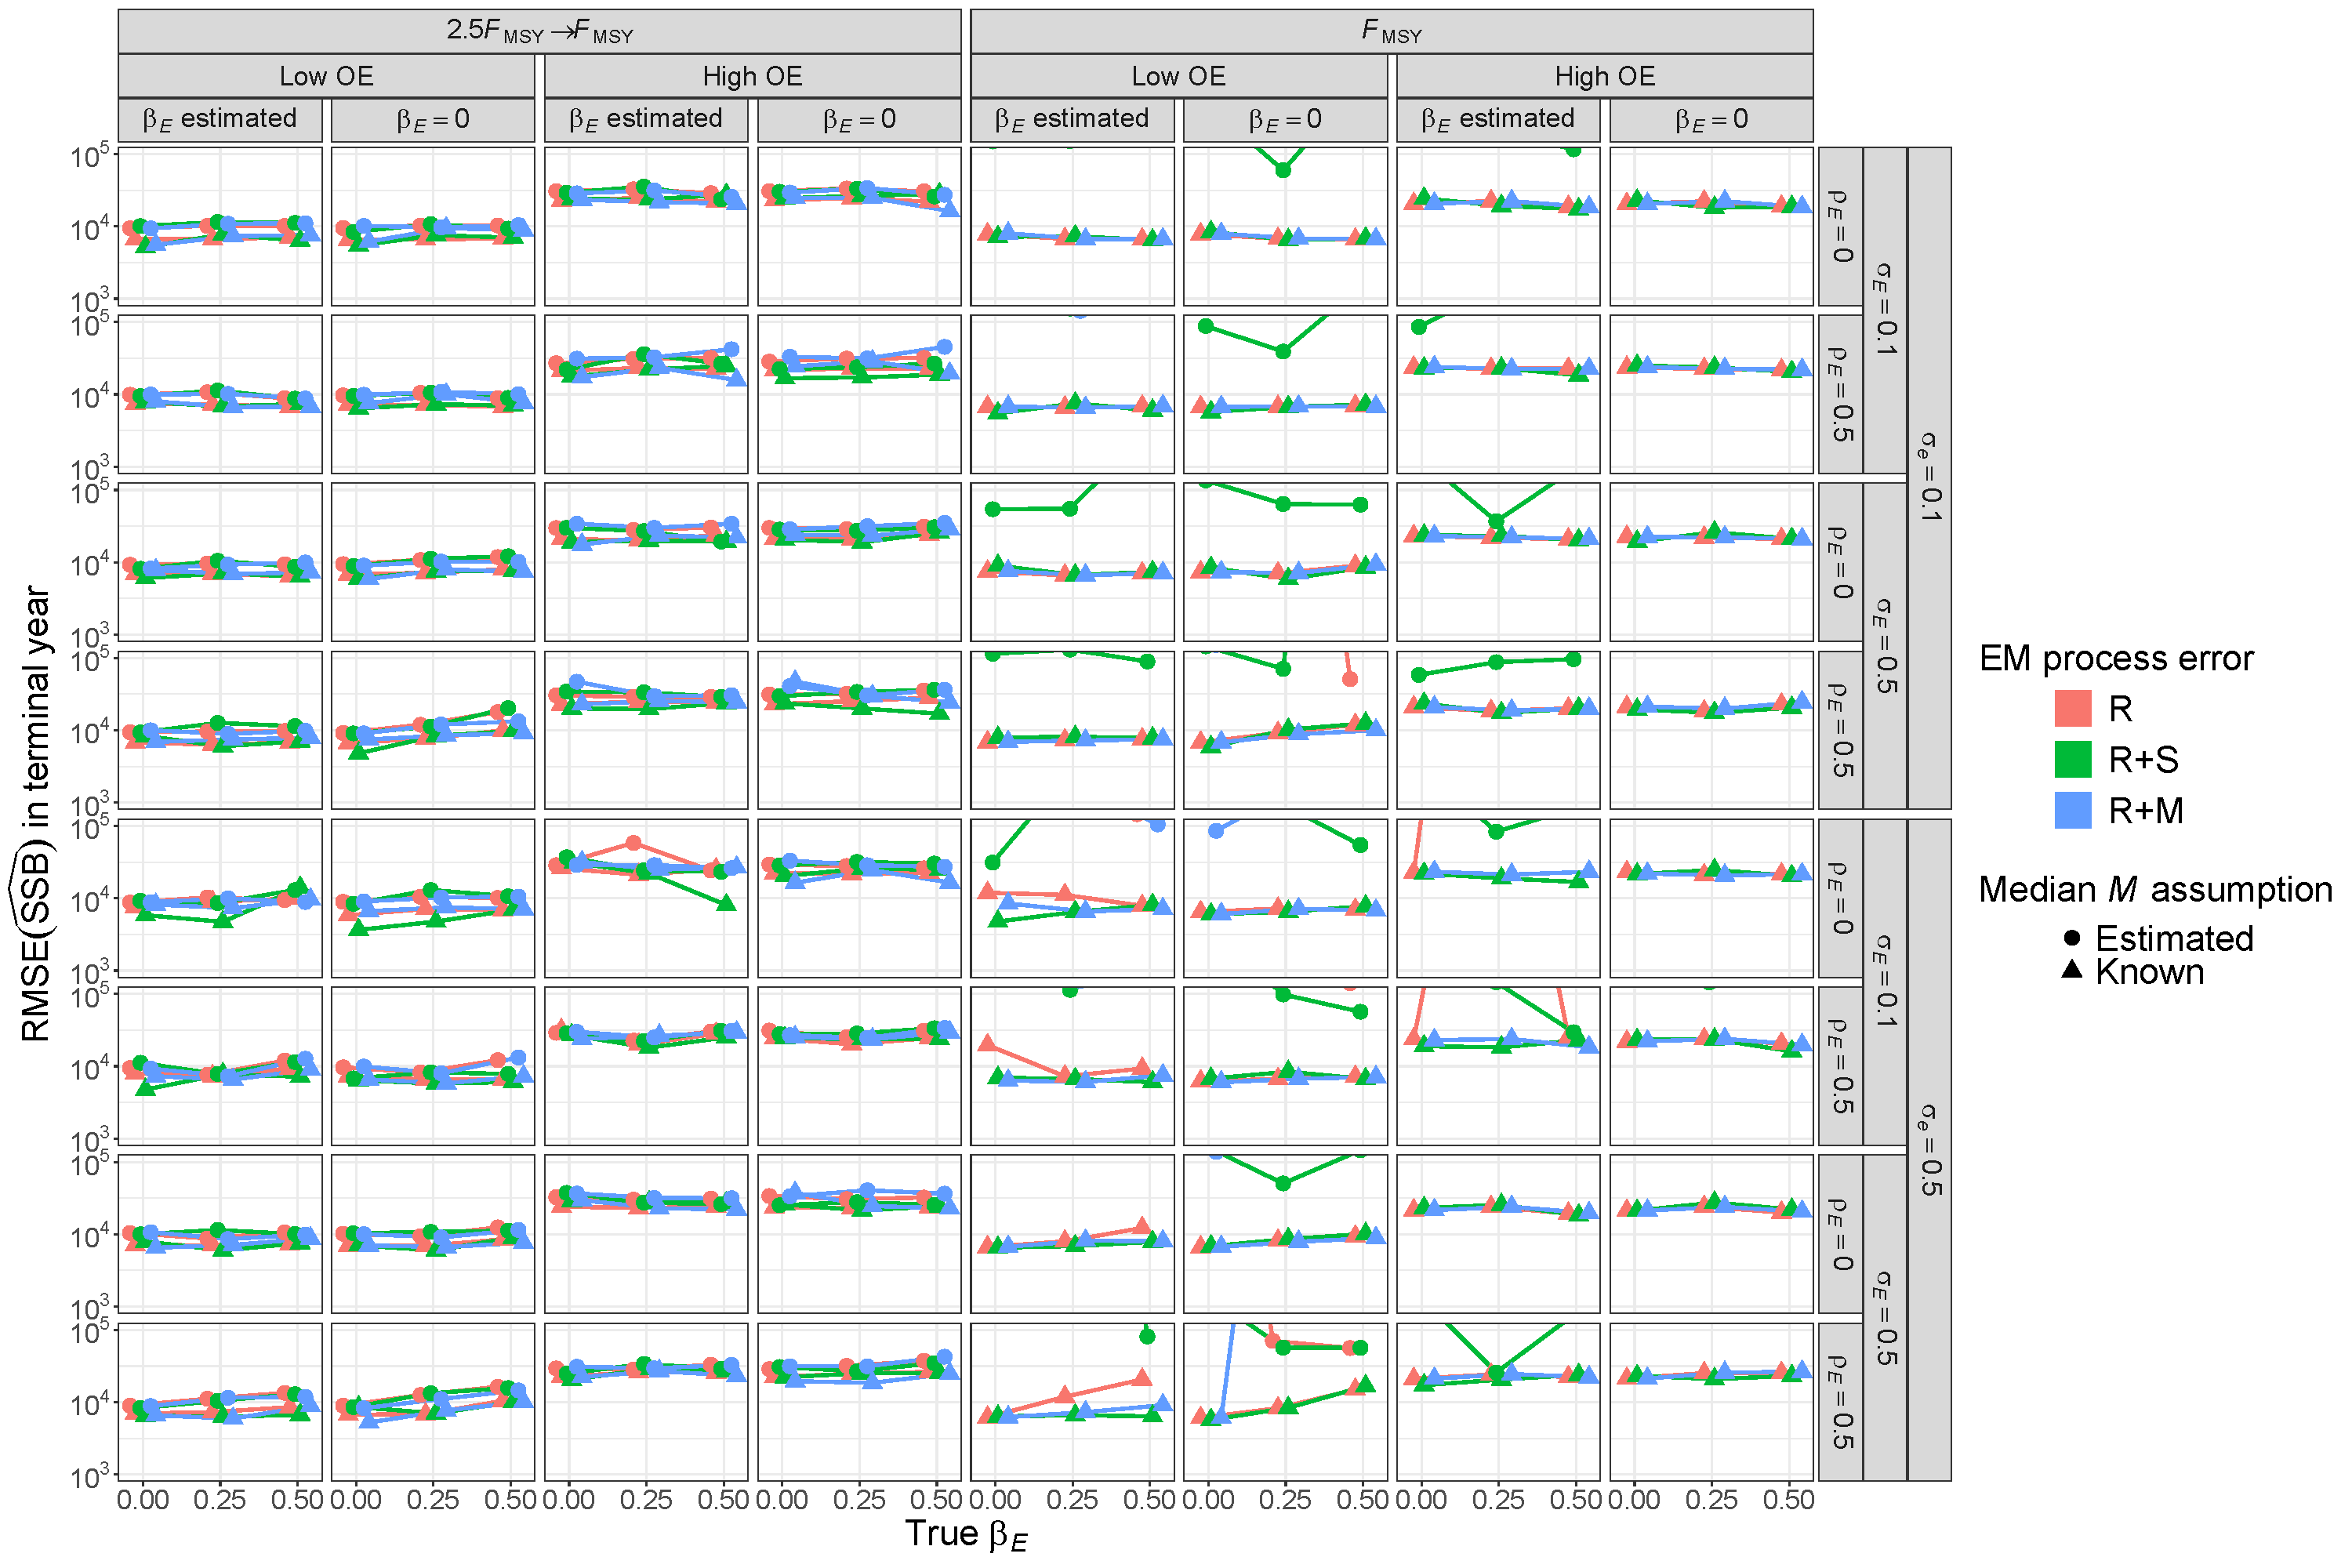
\includegraphics[height = \textheight]{terminal_year_ssb_rmse_Rom}
\end{center}
\caption{For R operating models, RMSE of estimates of SSB in the terminal year for estimating models with alternative process error assumptions, treatment of covariate effect ($\beta_E = 0$ or estimated), and treatment of median $M$ parameter ($\beta_M$ estimated or known).}\label{terminal_ssb_rmse_Rom}
\end{figure}
\end{landscape}

\begin{landscape}
\begin{figure}
\begin{center}
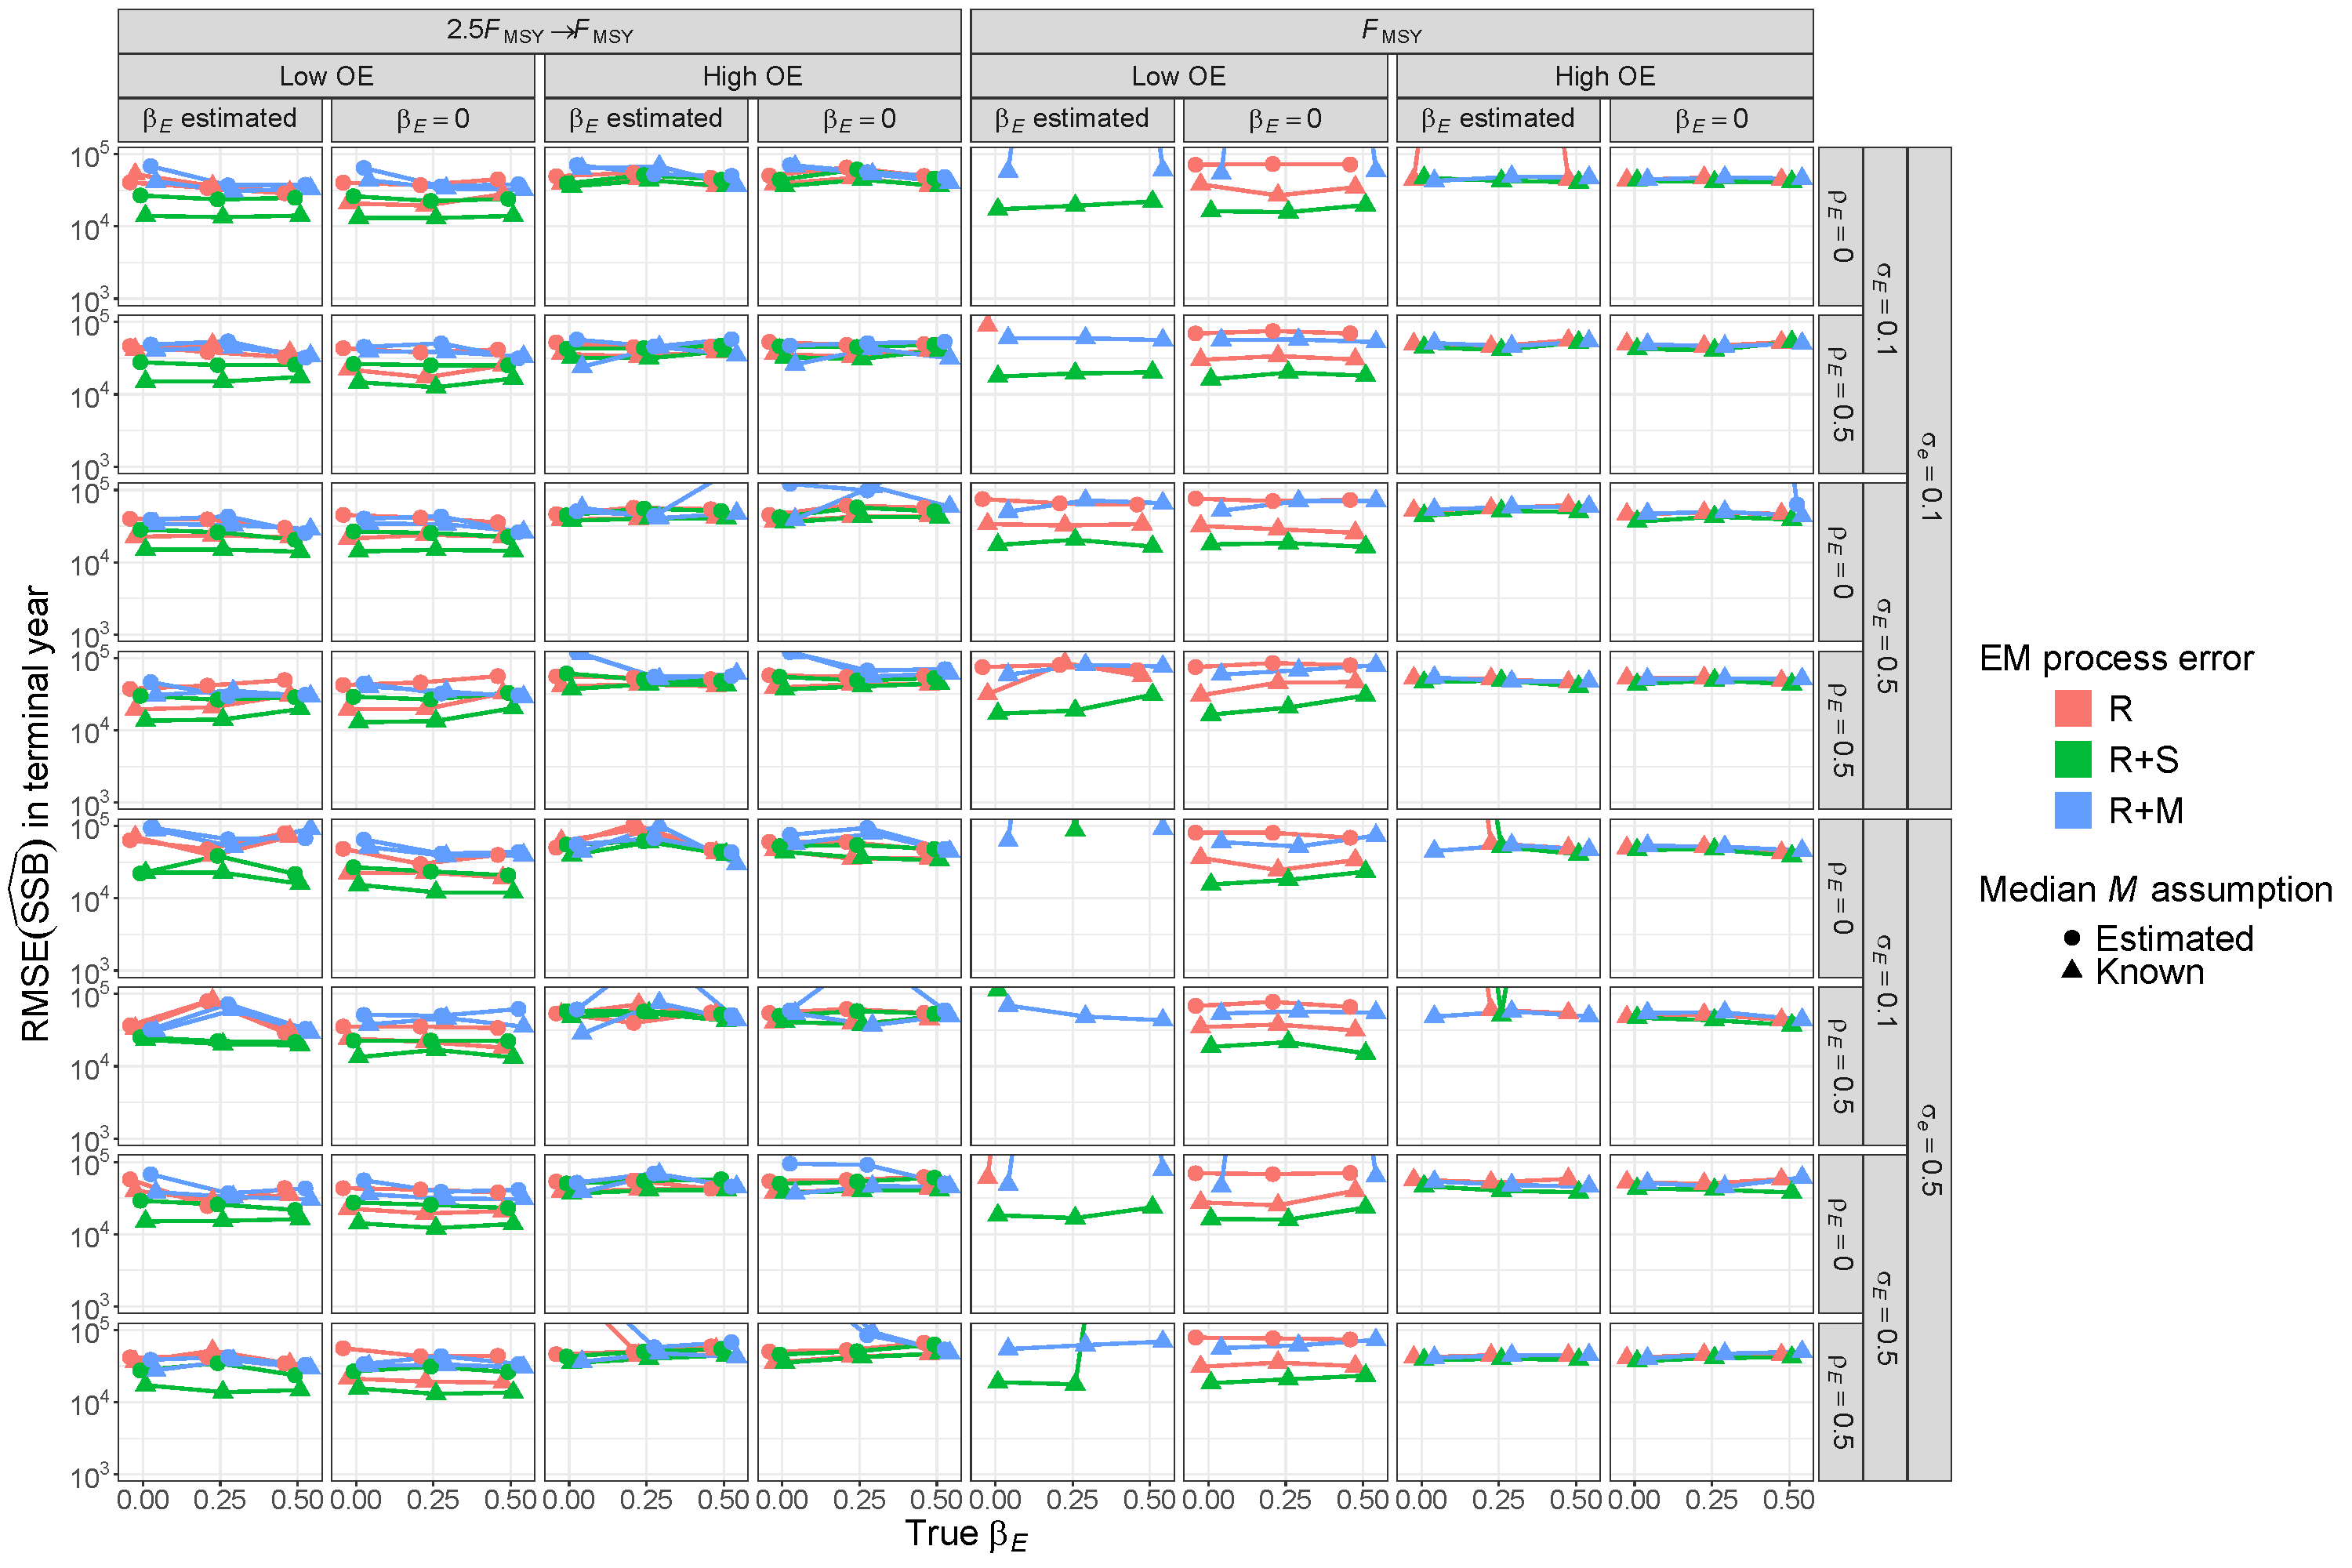
\includegraphics[height = \textheight]{terminal_year_ssb_rmse_RSom}
\end{center}
\caption{For R+S operating models, RMSE of estimates of SSB in the terminal year for estimating models with alternative process error assumptions, treatment of covariate effect ($\beta_E = 0$ or estimated), and treatment of median $M$ parameter ($\beta_M$ estimated or known).}\label{terminal_ssb_rmse_RSom}
\end{figure}
\end{landscape}

\begin{landscape}
\begin{figure}
\begin{center}
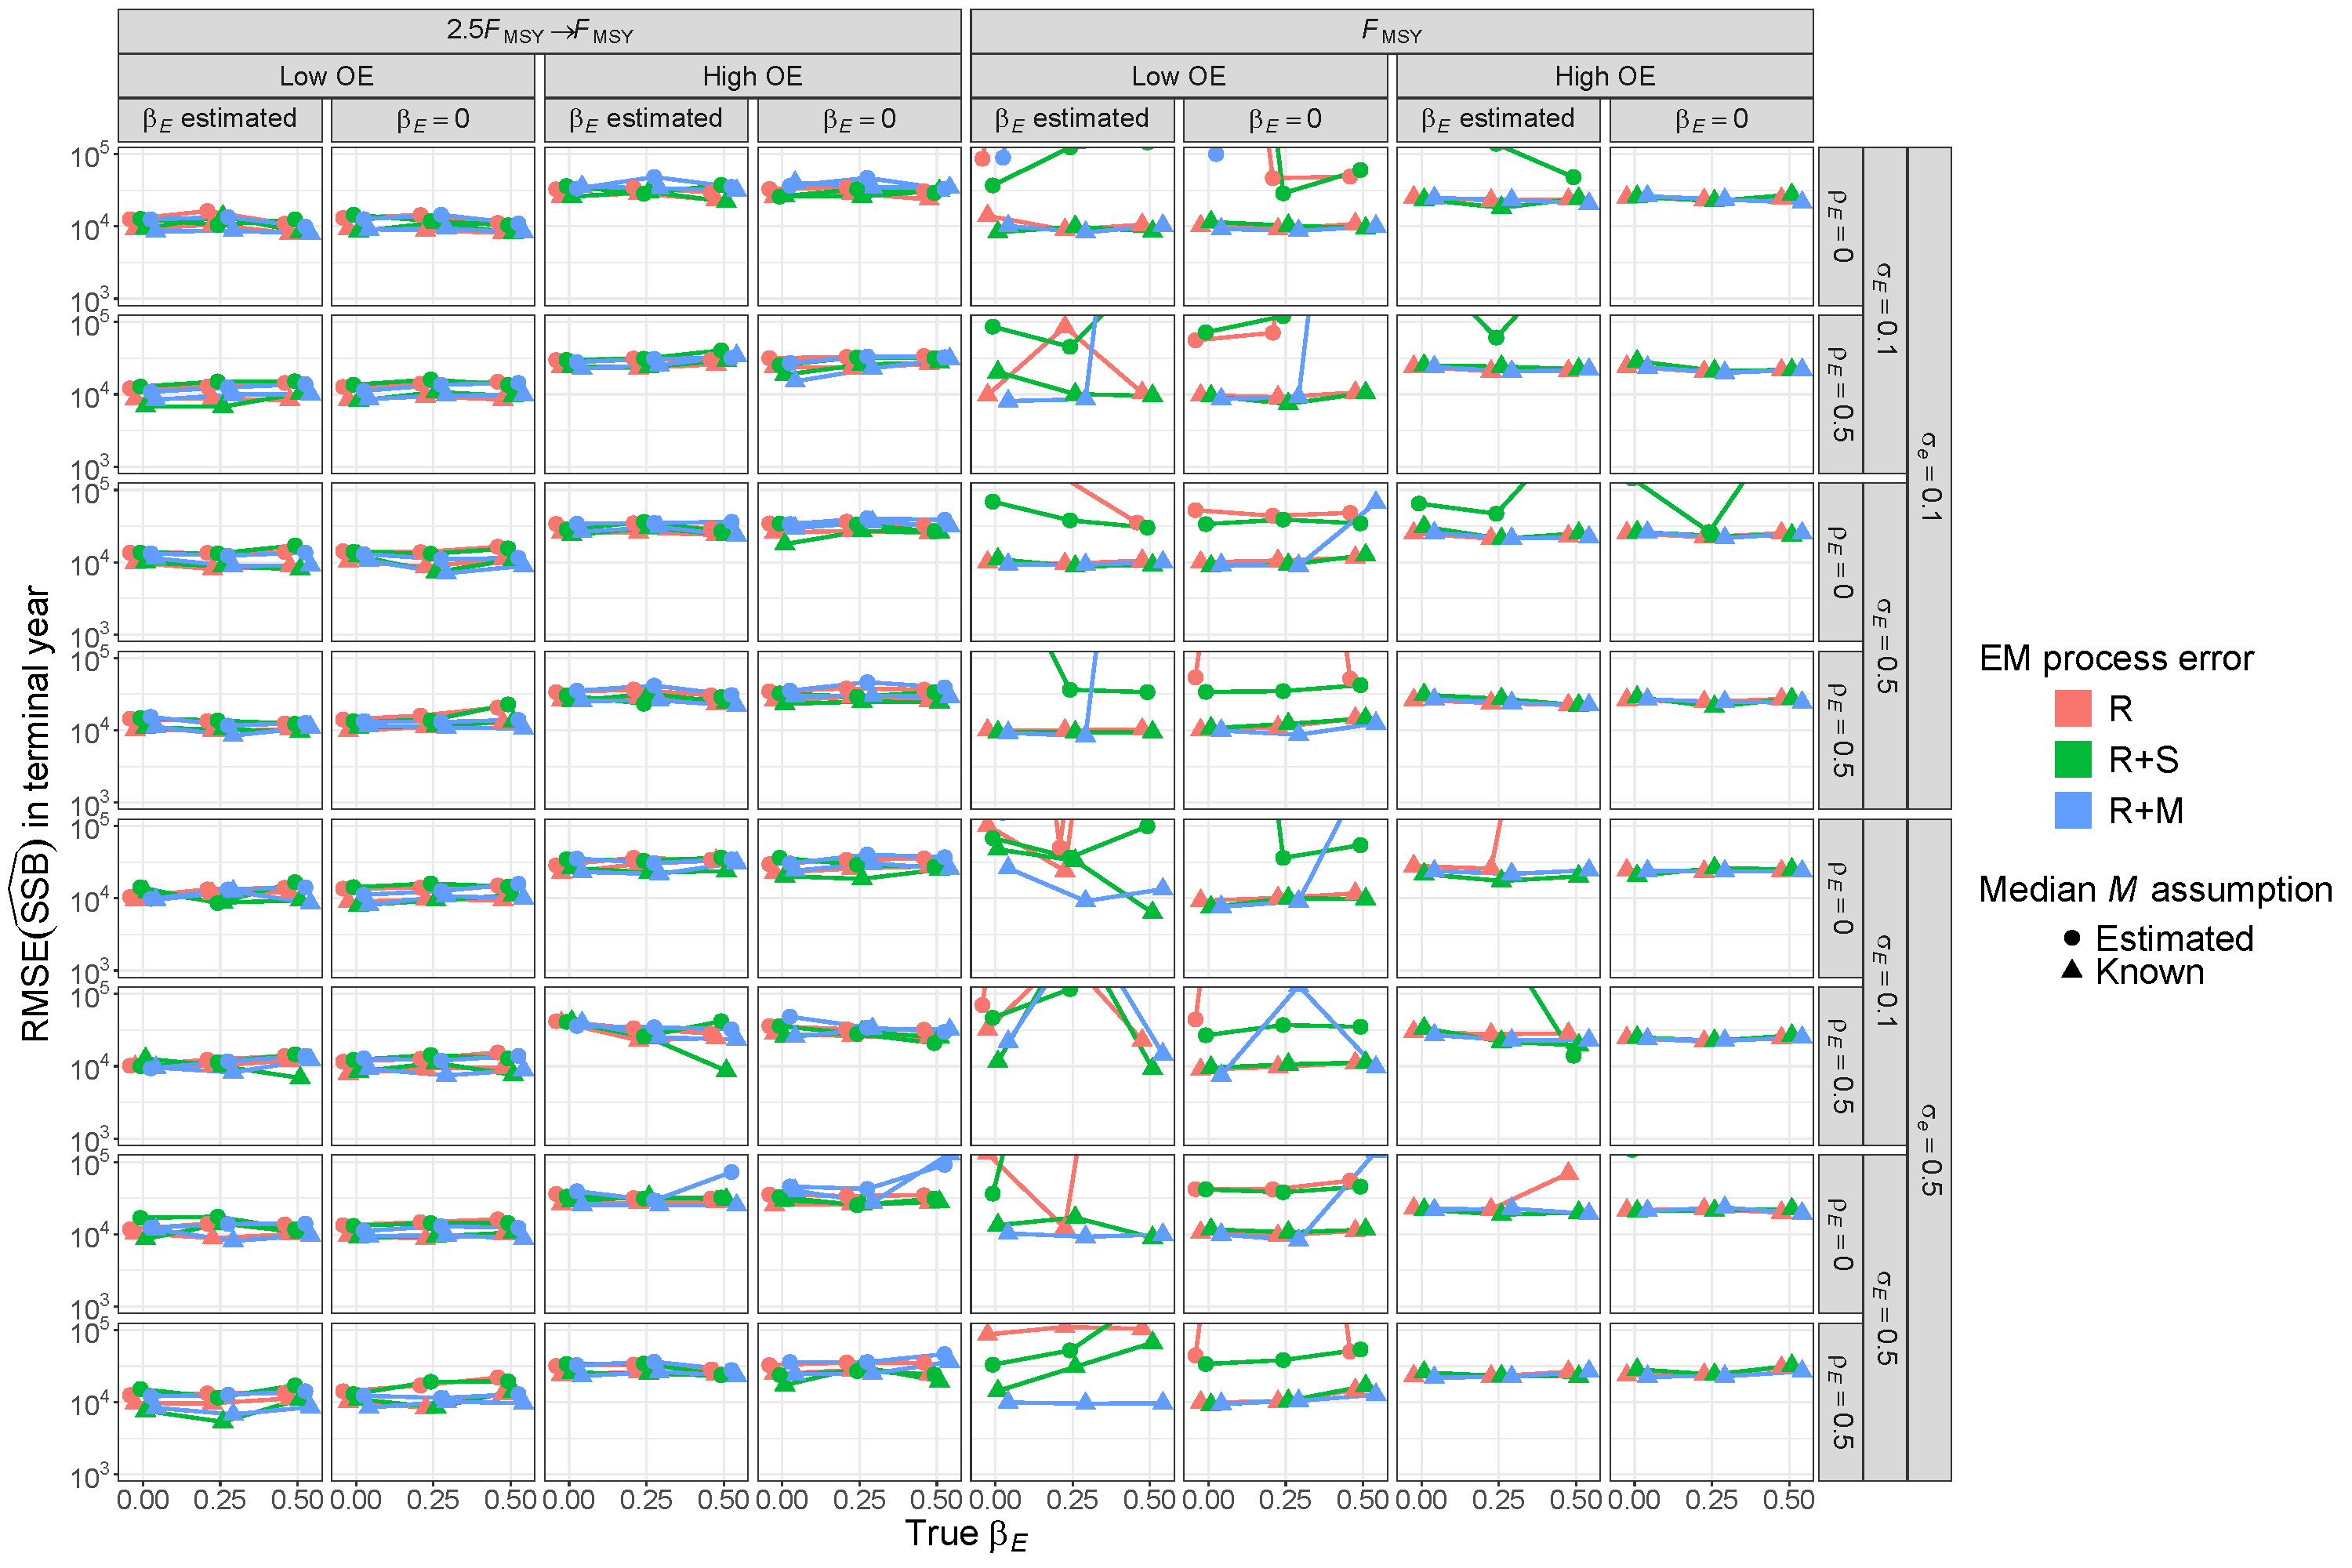
\includegraphics[height = \textheight]{terminal_year_ssb_rmse_RMom}
\end{center}
\caption{For R+M operating models, RMSE of estimates of SSB in the terminal year for estimating models with alternative process error assumptions, treatment of covariate effect ($\beta_E = 0$ or estimated), and treatment of median $M$ parameter ($\beta_M$ estimated or known).}\label{terminal_ssb_rmse_RMom}
\end{figure}
\end{landscape}

\begin{landscape}
\begin{figure}
\begin{center}
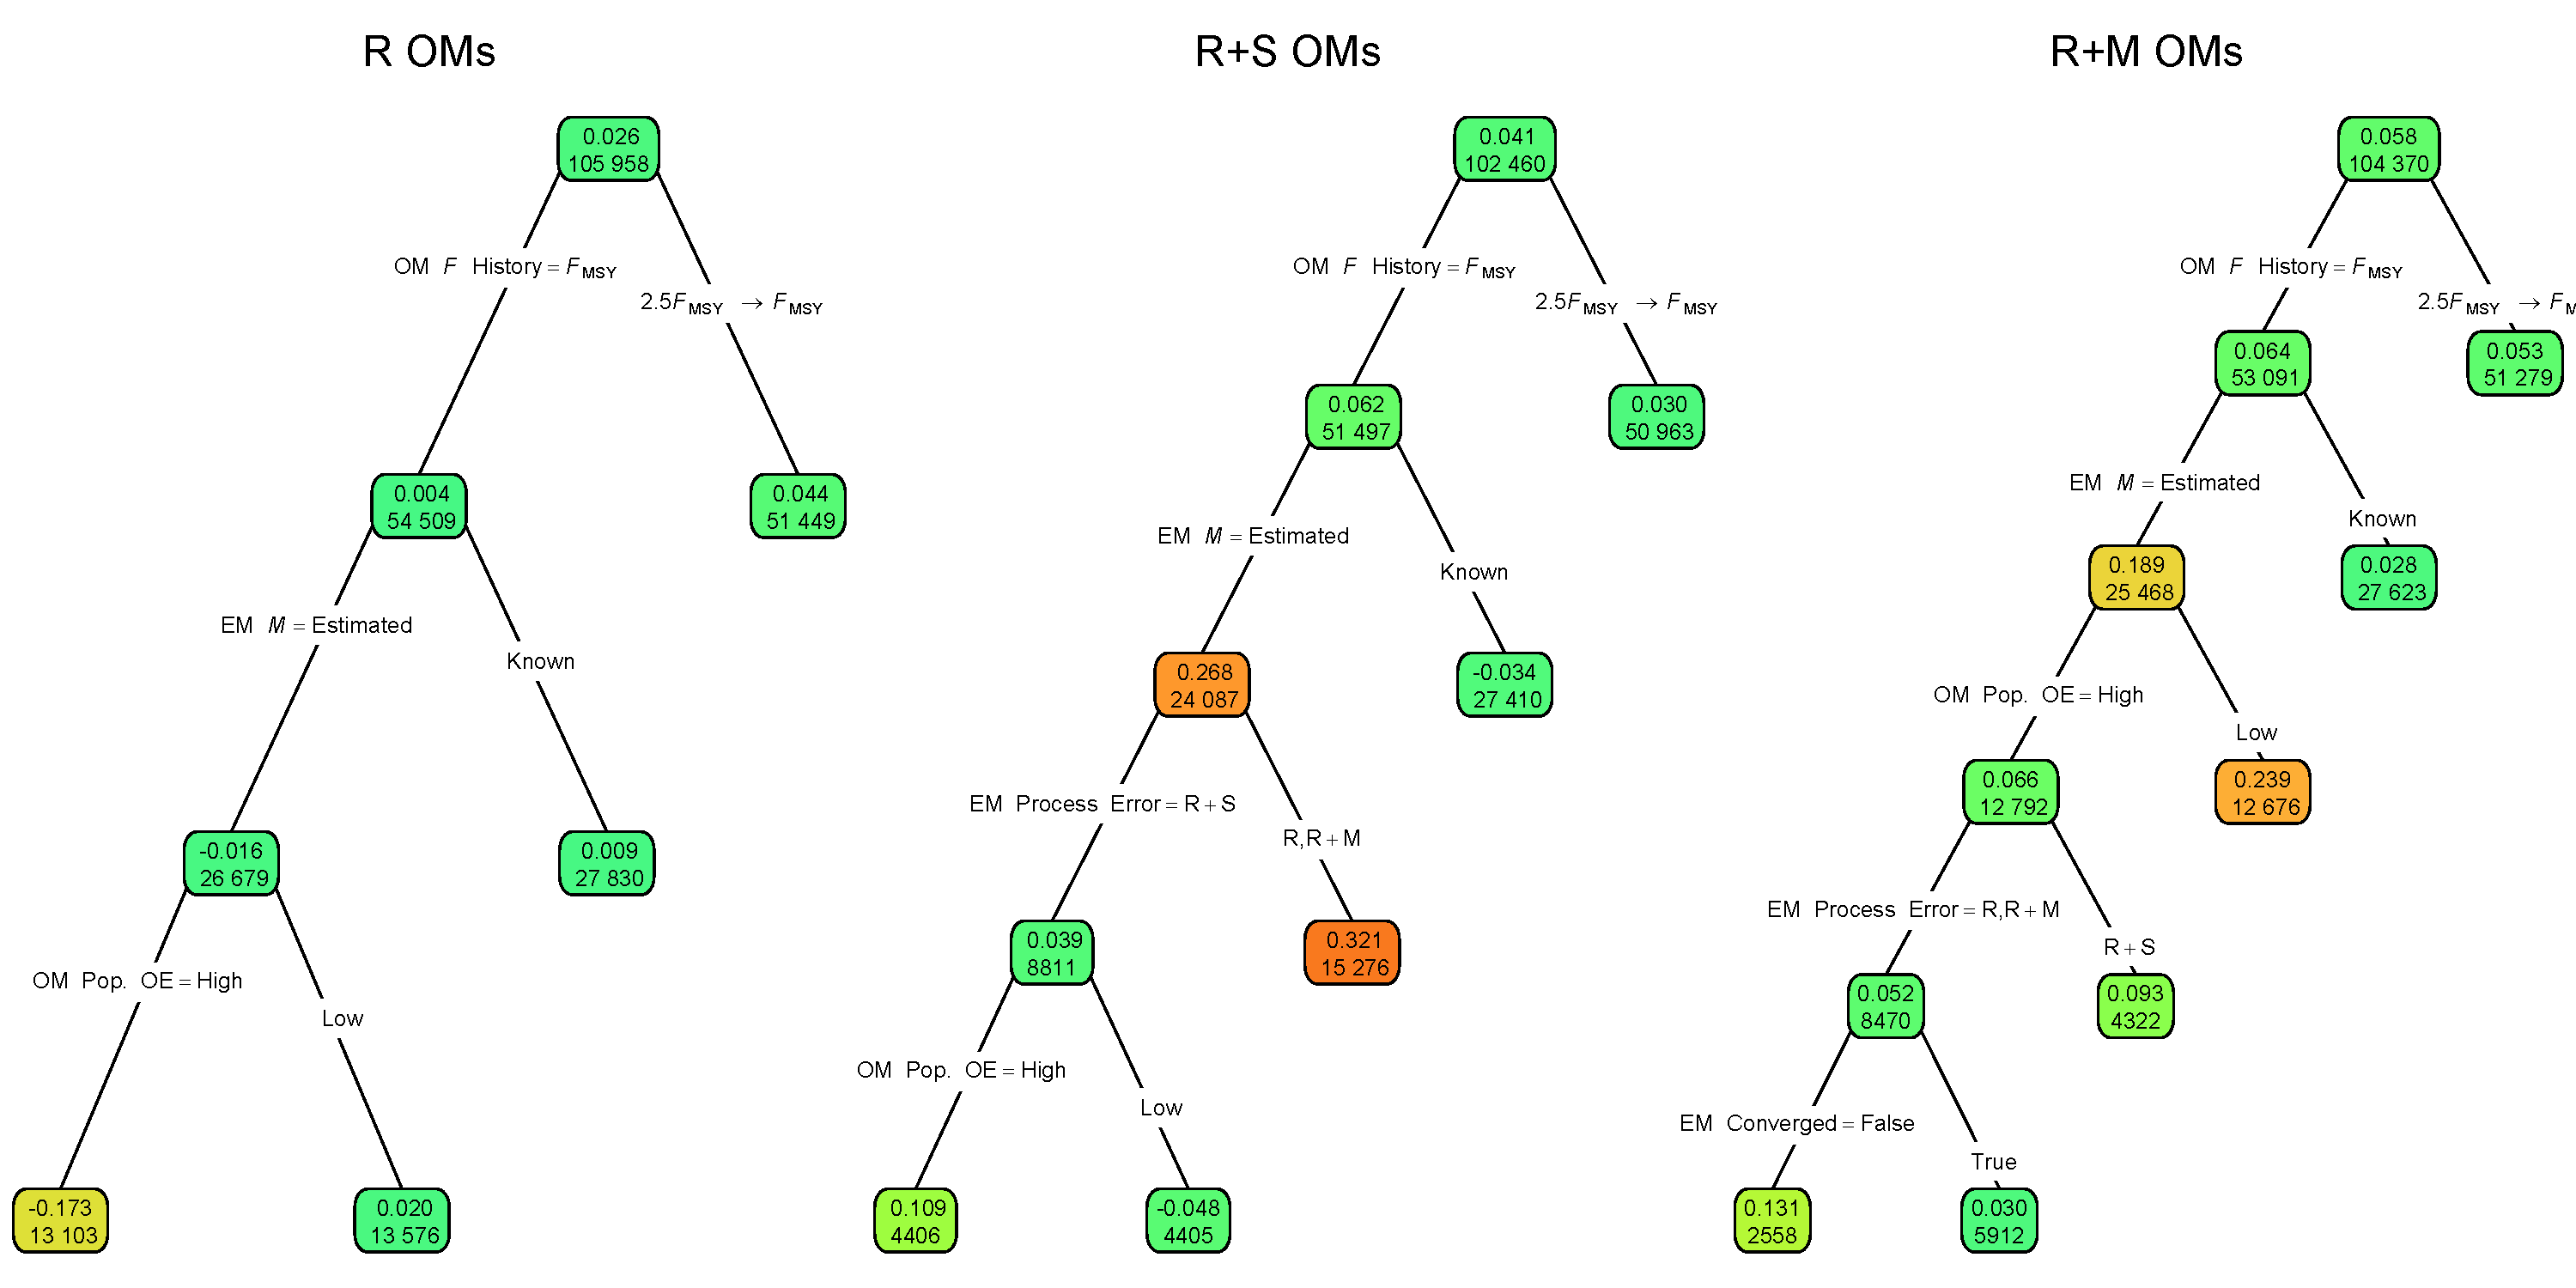
\includegraphics[width = 1.4\textwidth]{term_F_bias_regtree_plots}
\end{center}
\caption{Regression trees for errors terminal year fishing mortality rate as measured by Eq. \ref{relerror_trans_response}. Each node shows the median error for the corresponding subset. Lower or higher absolute median errors are indicated by more green or red polygons, respectively. See Figure \ref{conv_class} caption and Table \ref{factor_table} for further details.}\label{term_F_bias_regtree}
\end{figure}
\end{landscape}

\begin{table}
\caption{Percent reduction in deviance for linear regression models fit to errors in terminal year fishing mortality rate as measured by Eq. \ref{relerror_trans_response}. See Tables \ref{convergence_PRD_table} and \ref{factor_table} for further details.}\label{bias_F_PRD_table}
{\input{bias_F_PRD_table}}
\end{table}

\begin{landscape}
\begin{figure}
\begin{center}
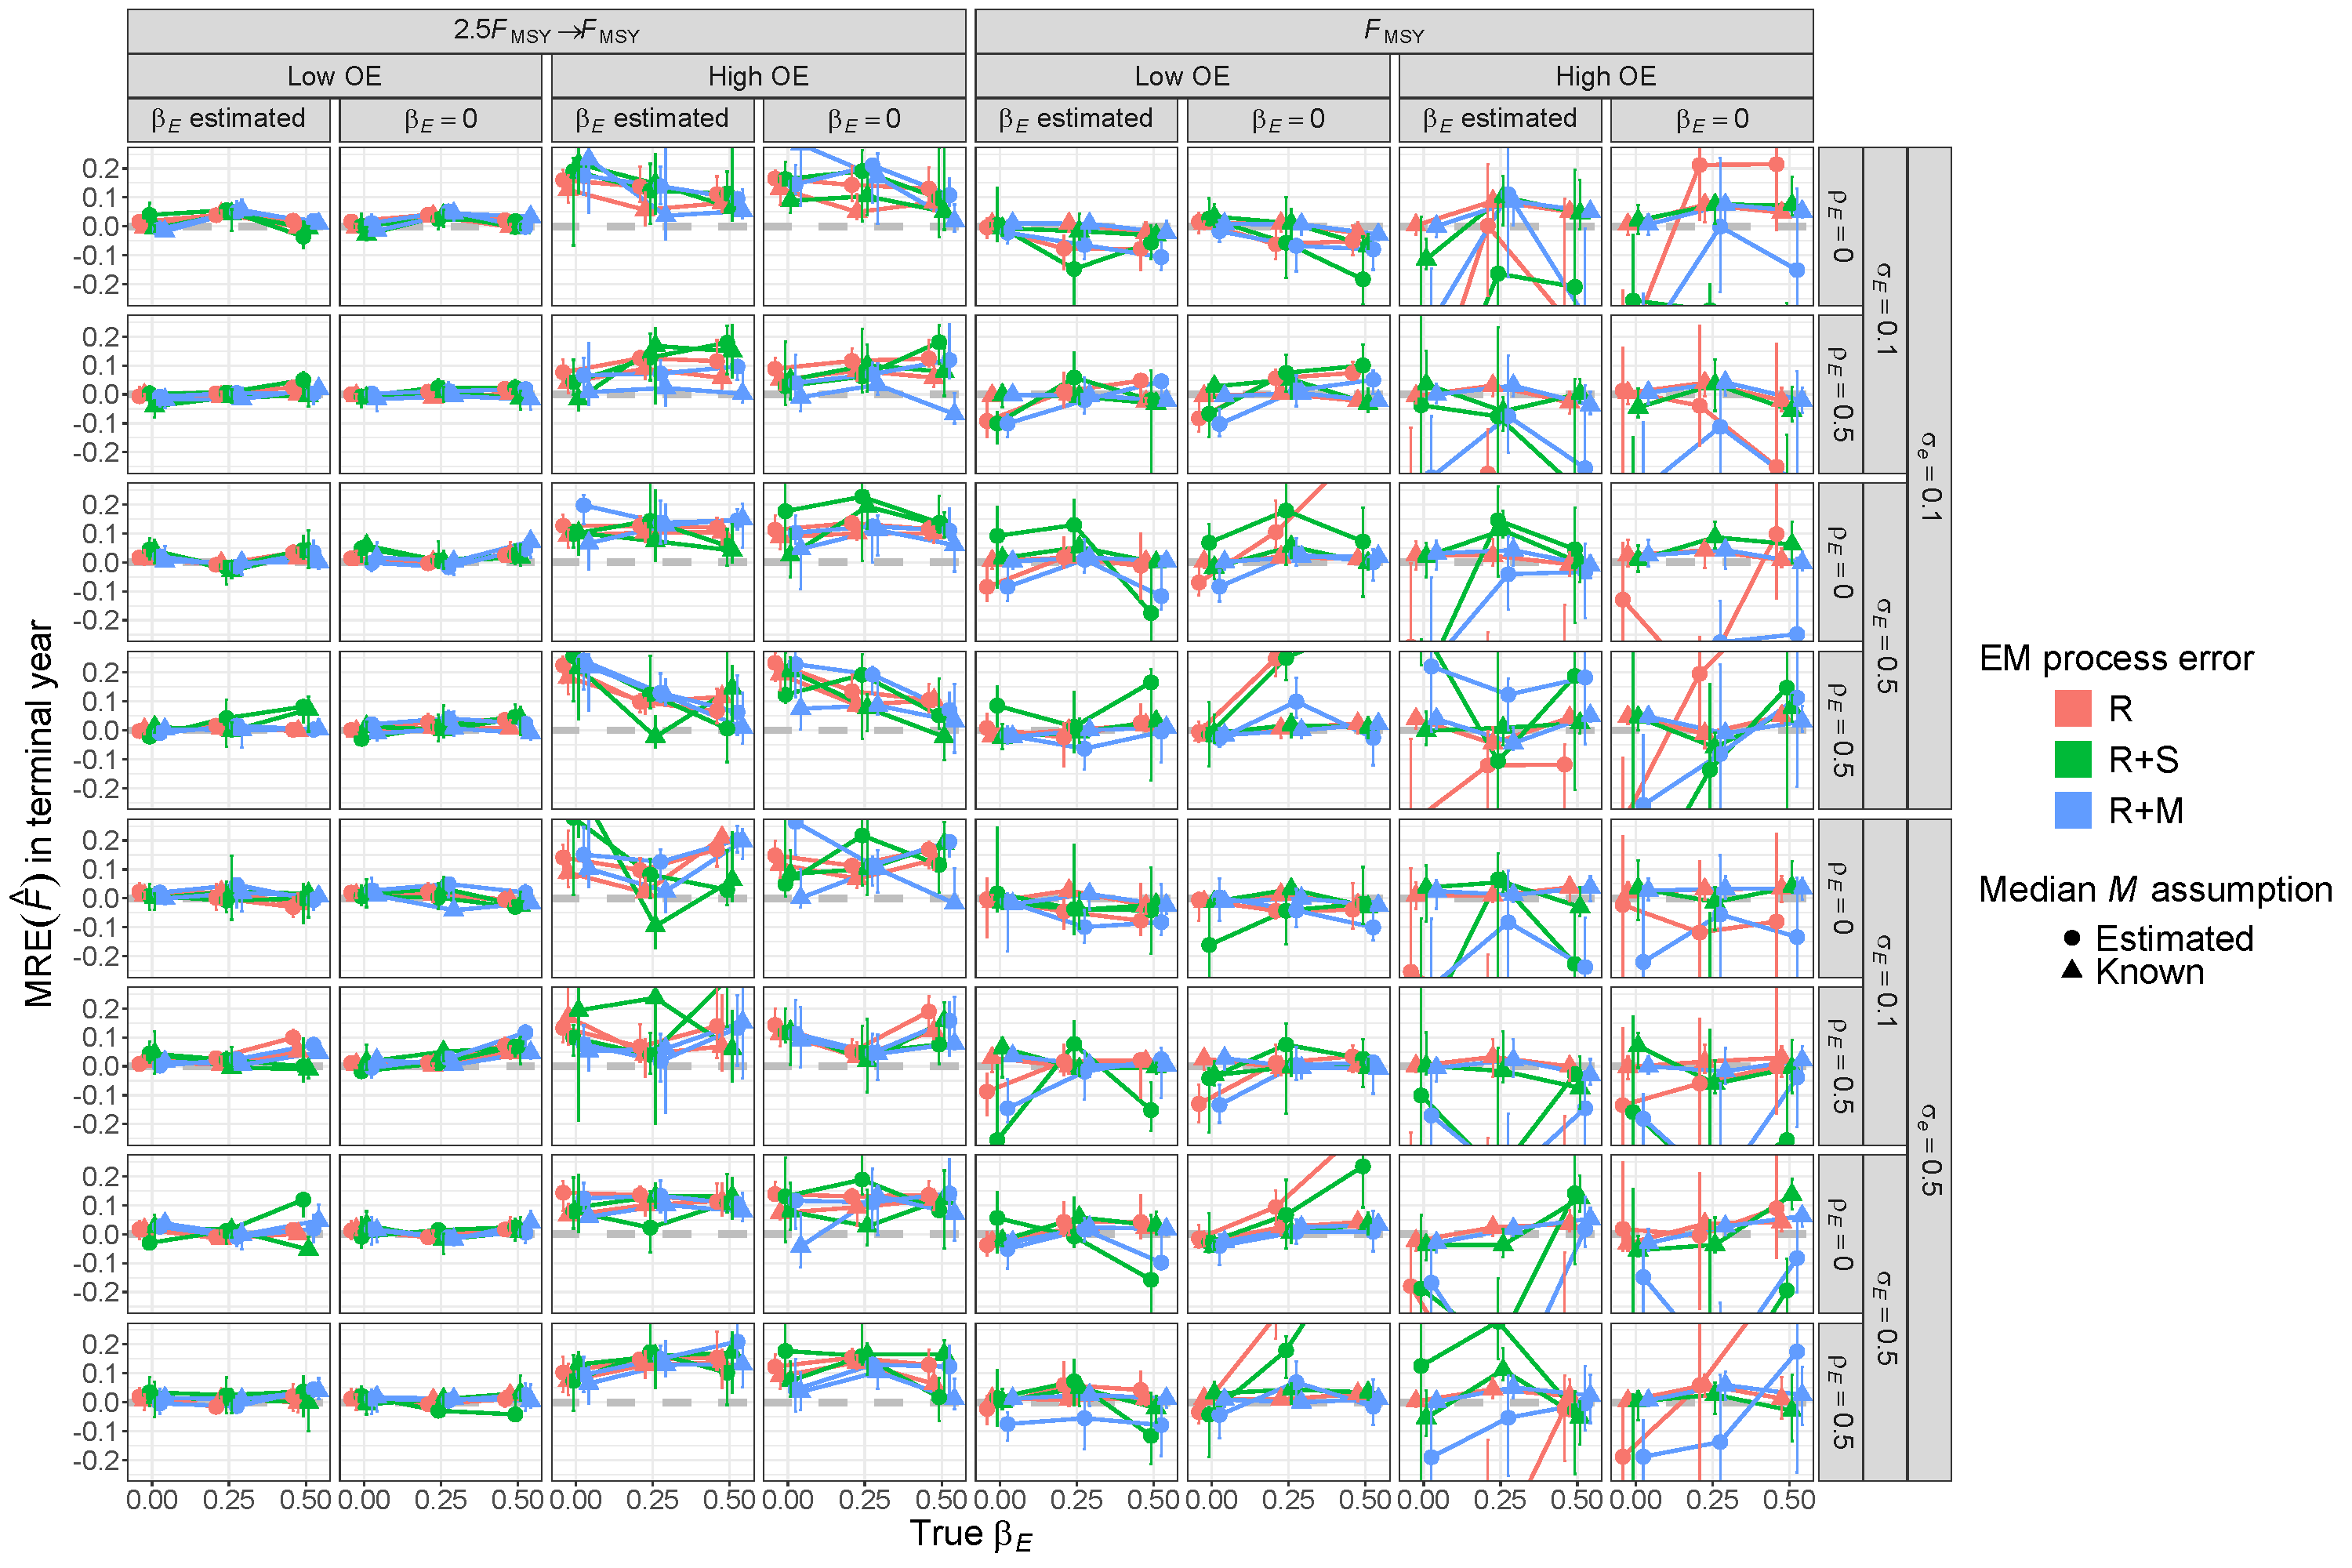
\includegraphics[height = \textheight]{terminal_year_F_bias_Rom}
\end{center}
\caption{For R operating models, median relative error (MRE) of estimates of fully-selected fishing mortality ($F$) in the terminal year for estimating models with alternative process error assumptions, treatment of covariate effect ($\beta_E = 0$ or estimated), and treatment of median $M$ parameter ($\beta_M$ estimated or known).}\label{terminal_F_bias_Rom}
\end{figure}
\end{landscape}

\begin{landscape}
\begin{figure}
\begin{center}
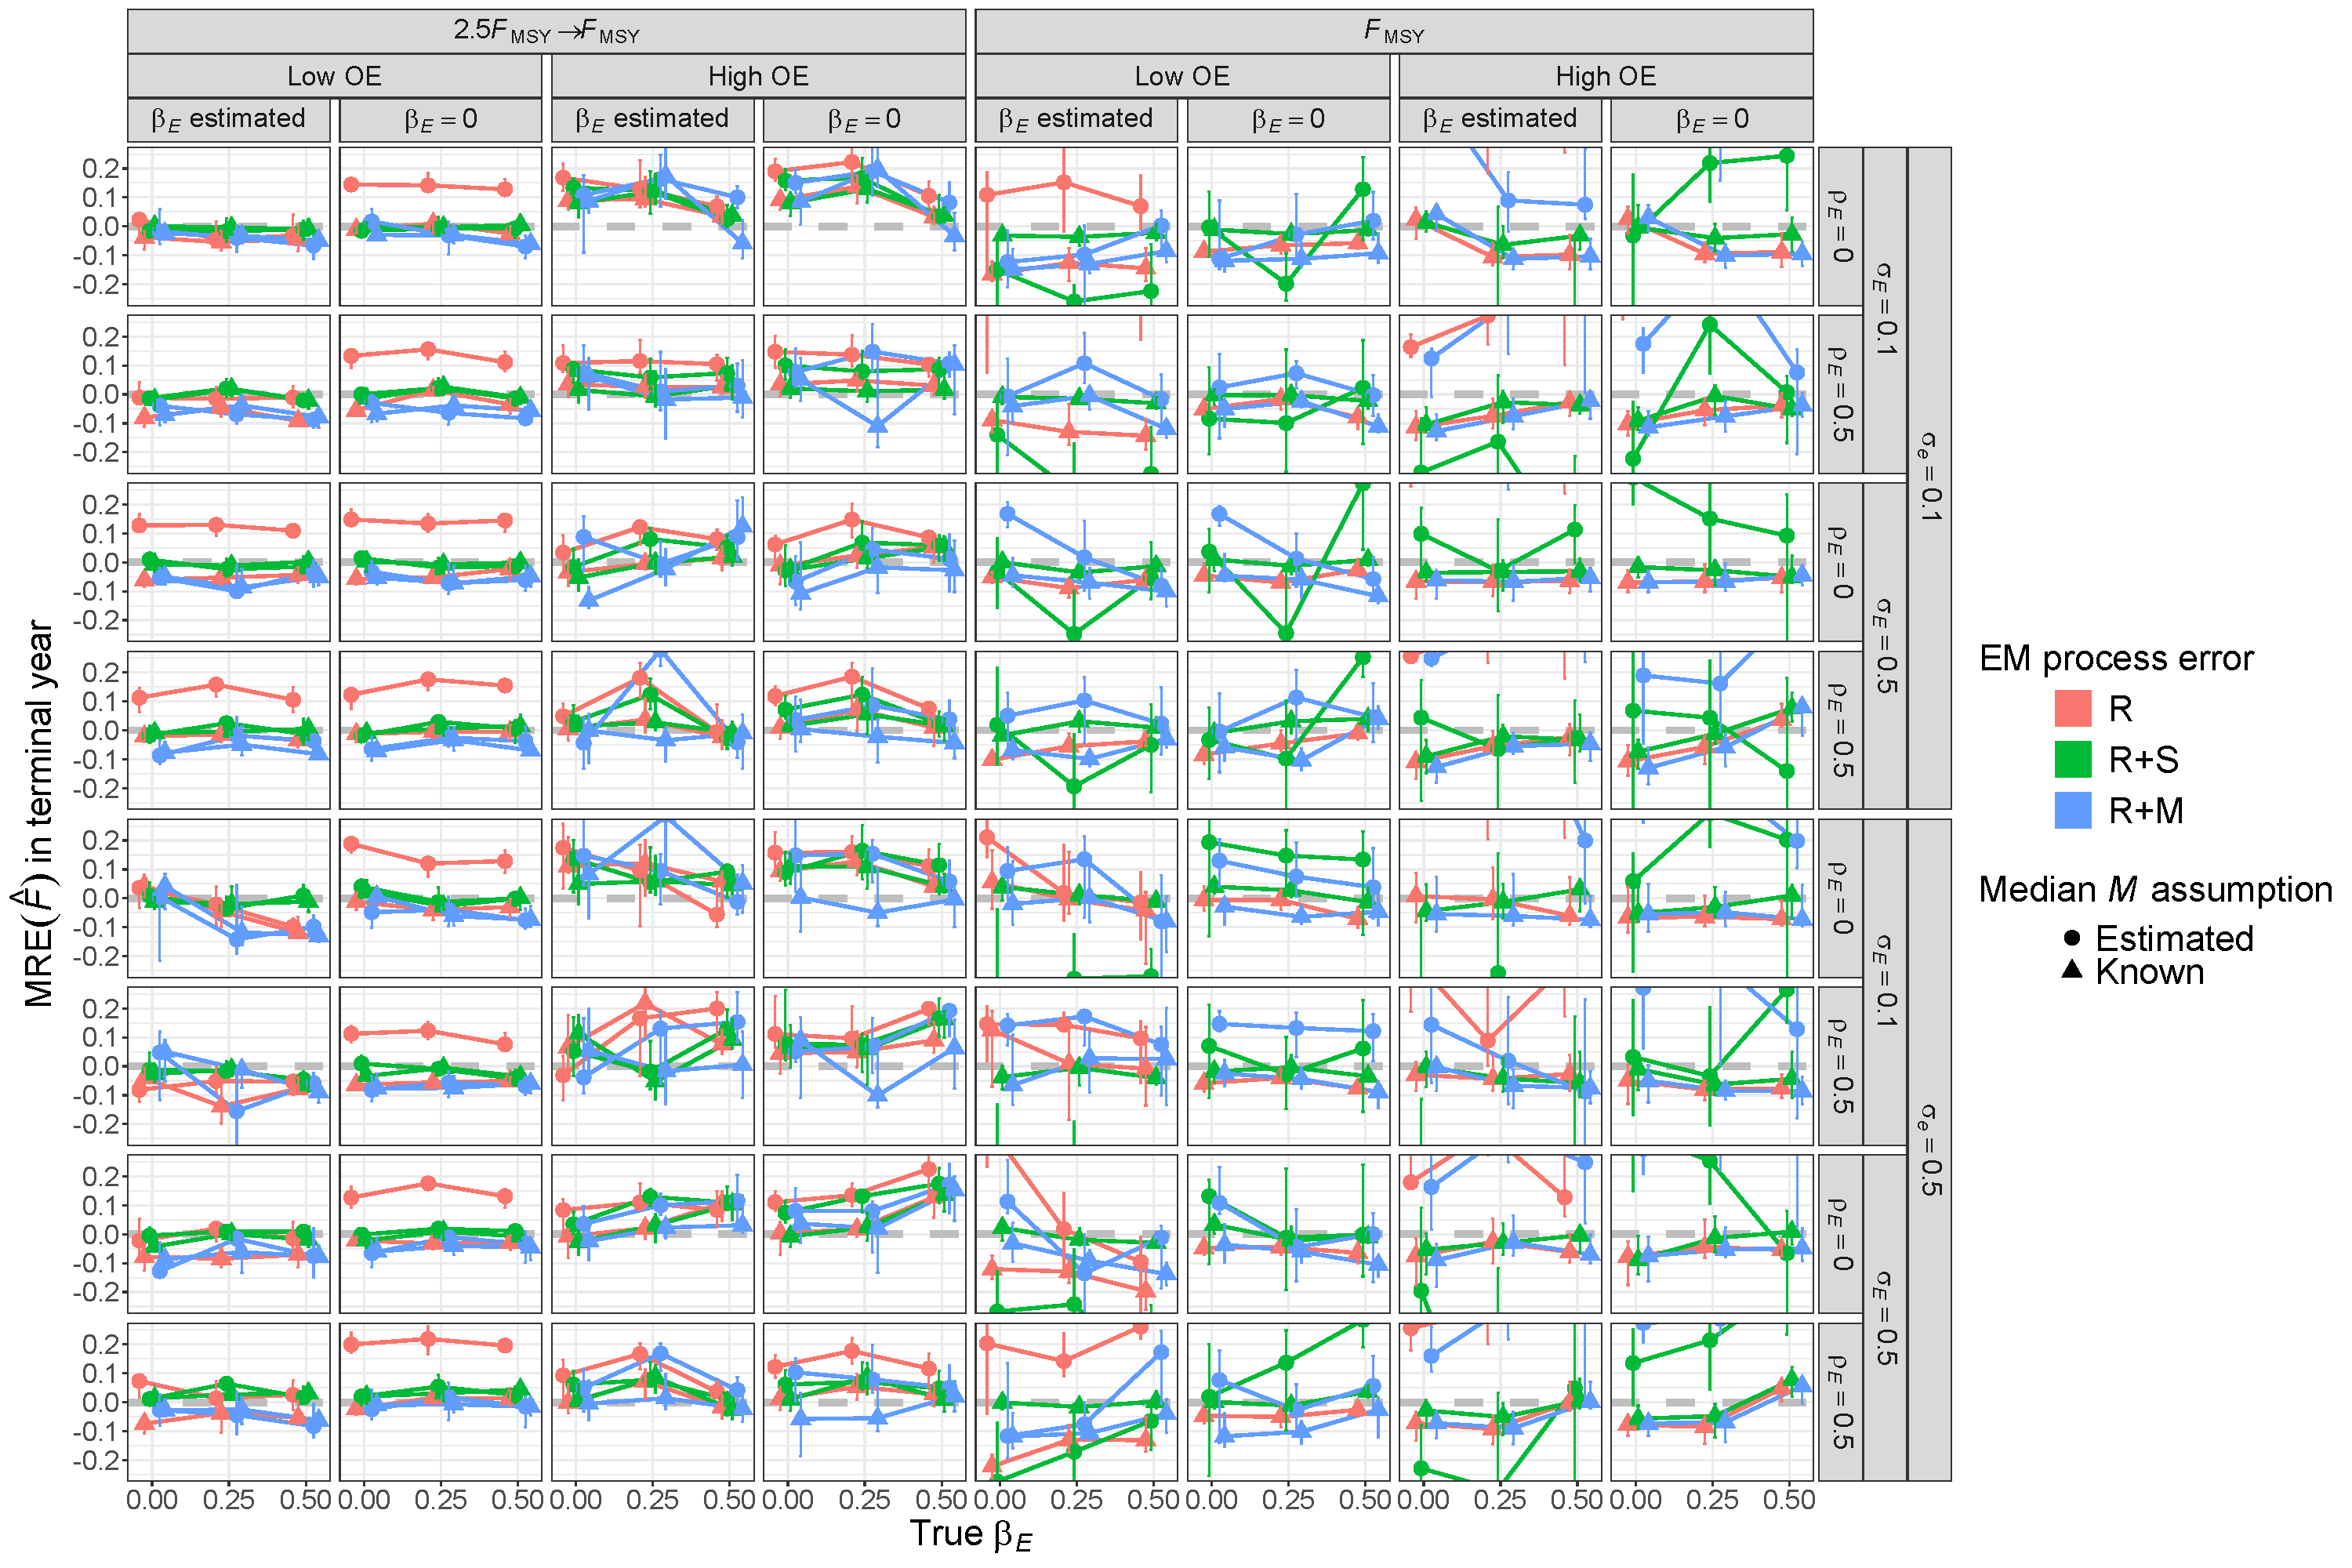
\includegraphics[height = \textheight]{terminal_year_F_bias_RSom}
\end{center}
\caption{For R+S operating models, median relative error (MRE) of estimates of fully-selected fishing mortality ($F$) in the terminal year for estimating models with alternative process error assumptions, treatment of covariate effect ($\beta_E = 0$ or estimated), and treatment of median $M$ parameter ($\beta_M$ estimated or known).}\label{terminal_F_bias_RSom}
\end{figure}
\end{landscape}

\begin{landscape}
\begin{figure}
\begin{center}
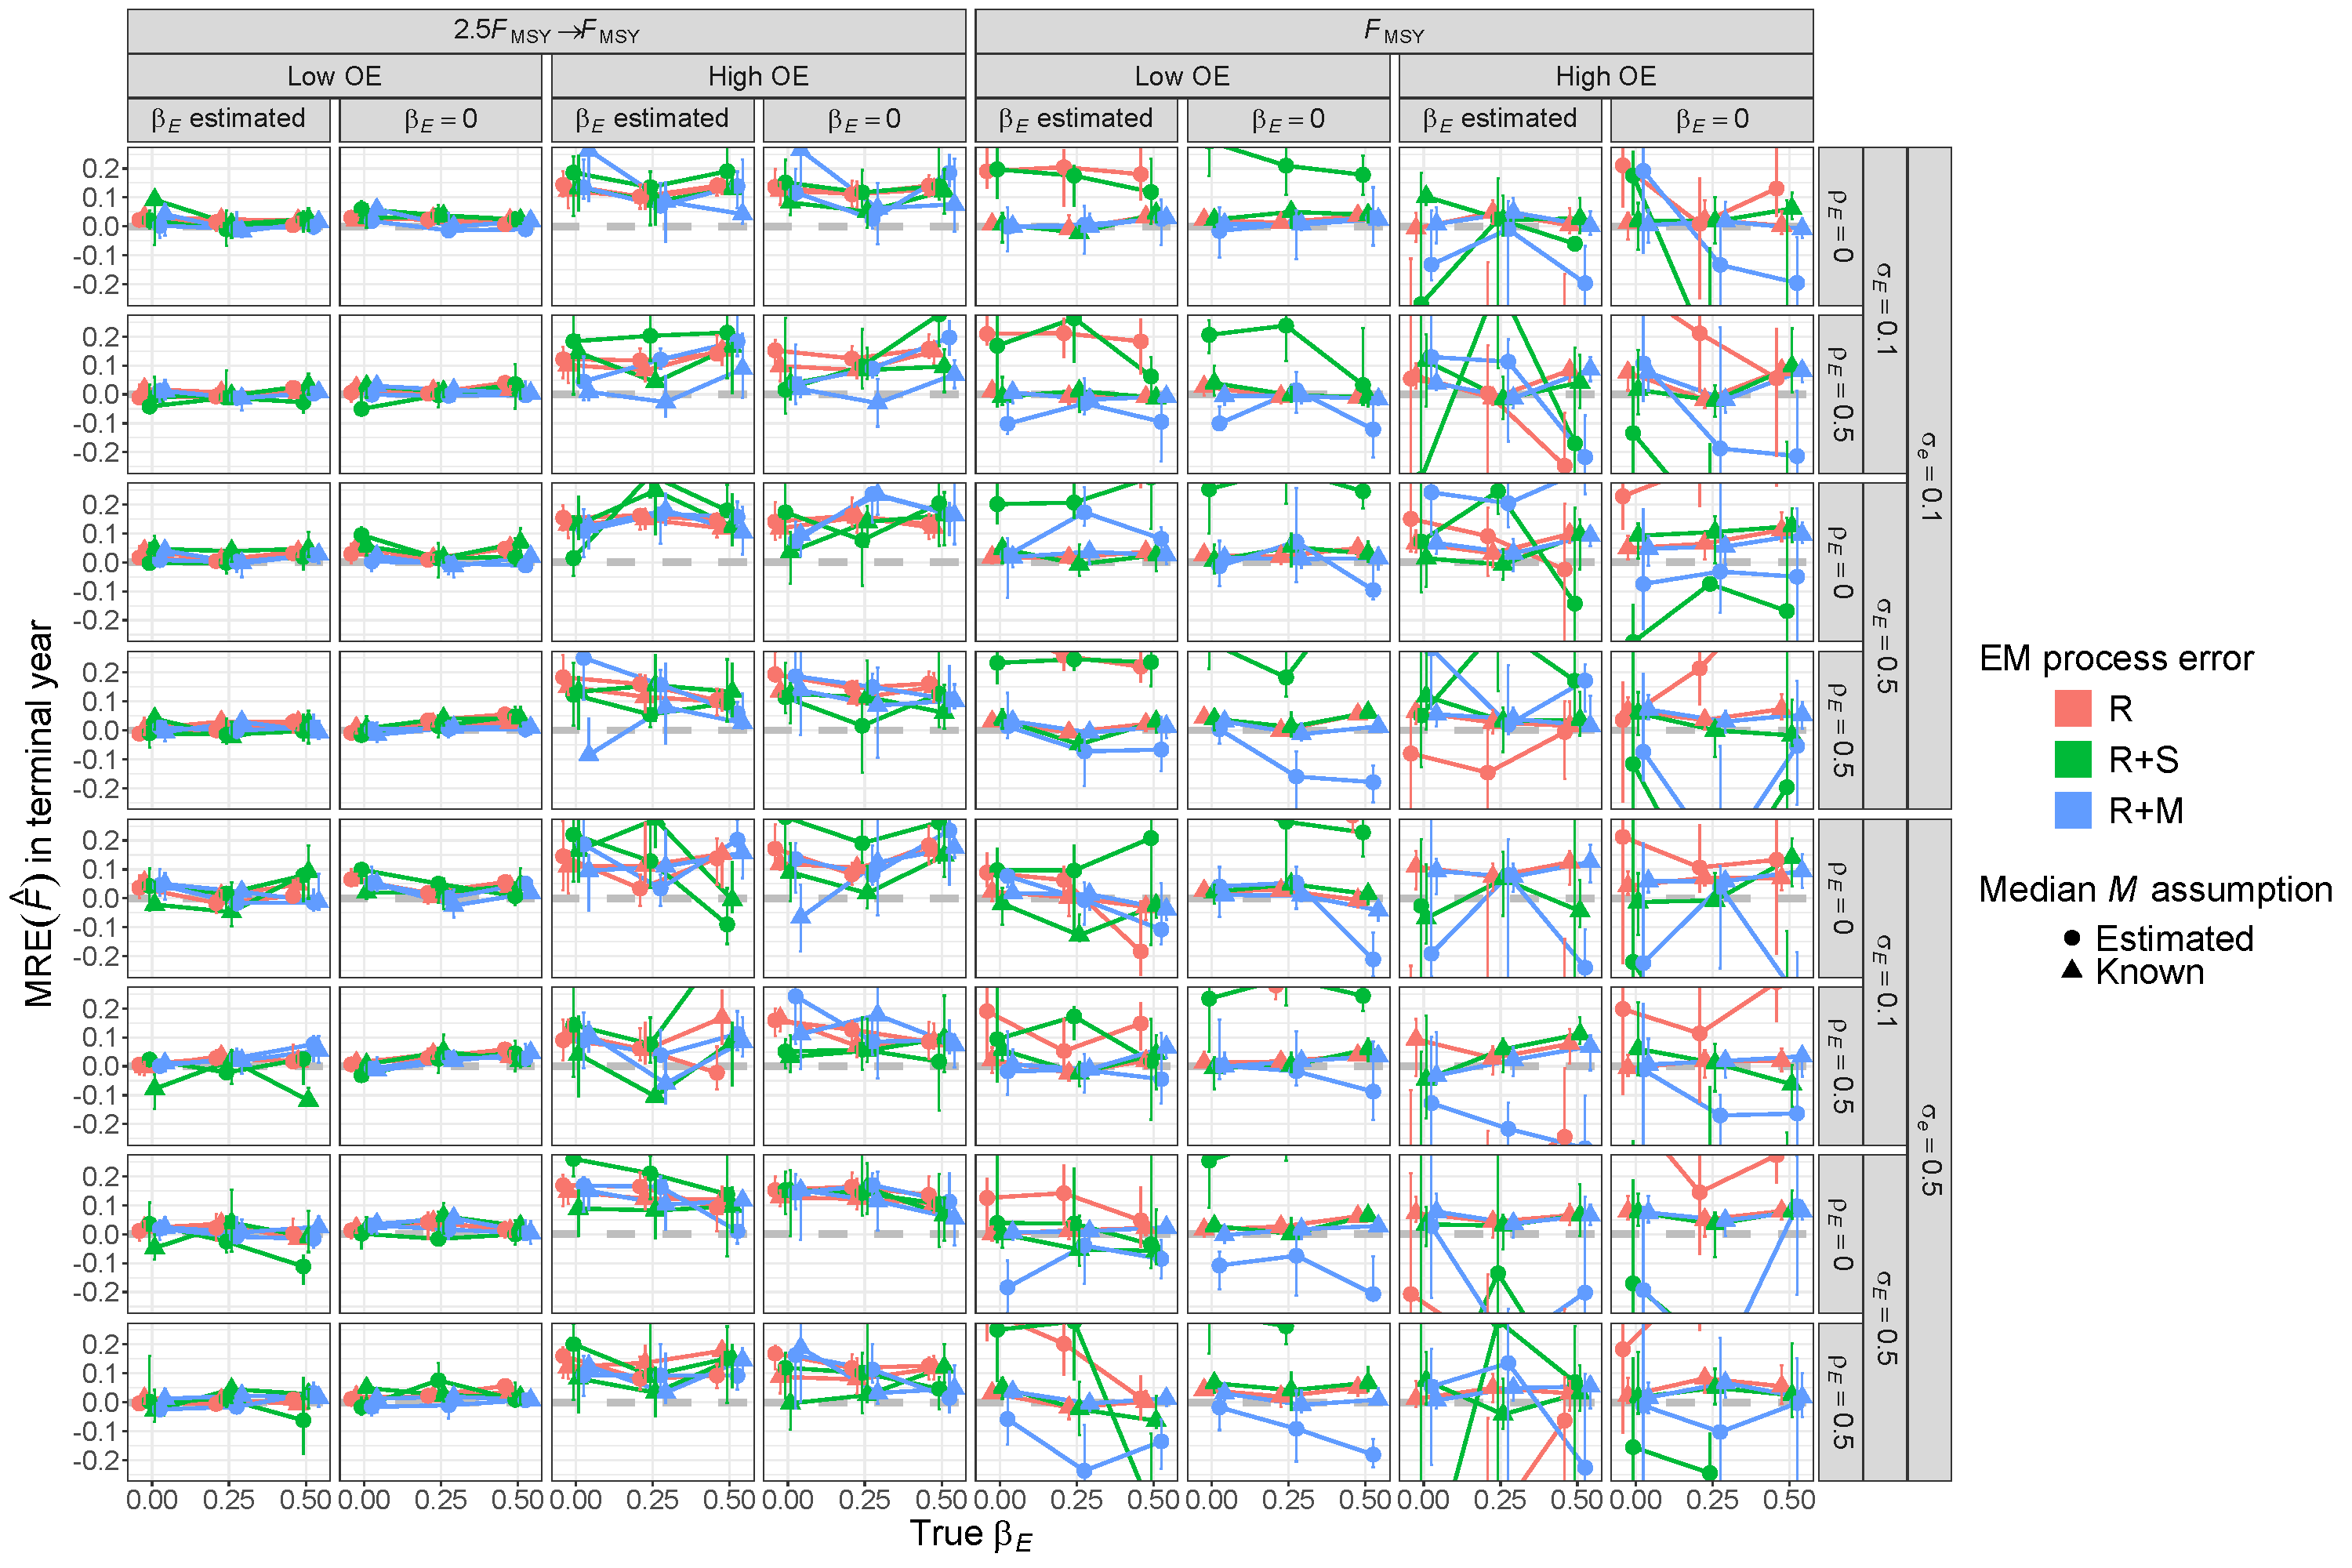
\includegraphics[height = \textheight]{terminal_year_F_bias_RMom}
\end{center}
\caption{For R+M operating models, median relative error (MRE) of estimates of fully-selected fishing mortality ($F$) in the terminal year for estimating models with alternative process error assumptions, treatment of covariate effect ($\beta_E = 0$ or estimated), and treatment of median $M$ parameter ($\beta_M$ estimated or known).}\label{terminal_F_bias_RMom}
\end{figure}
\end{landscape}

\begin{landscape}
\begin{figure}
\begin{center}
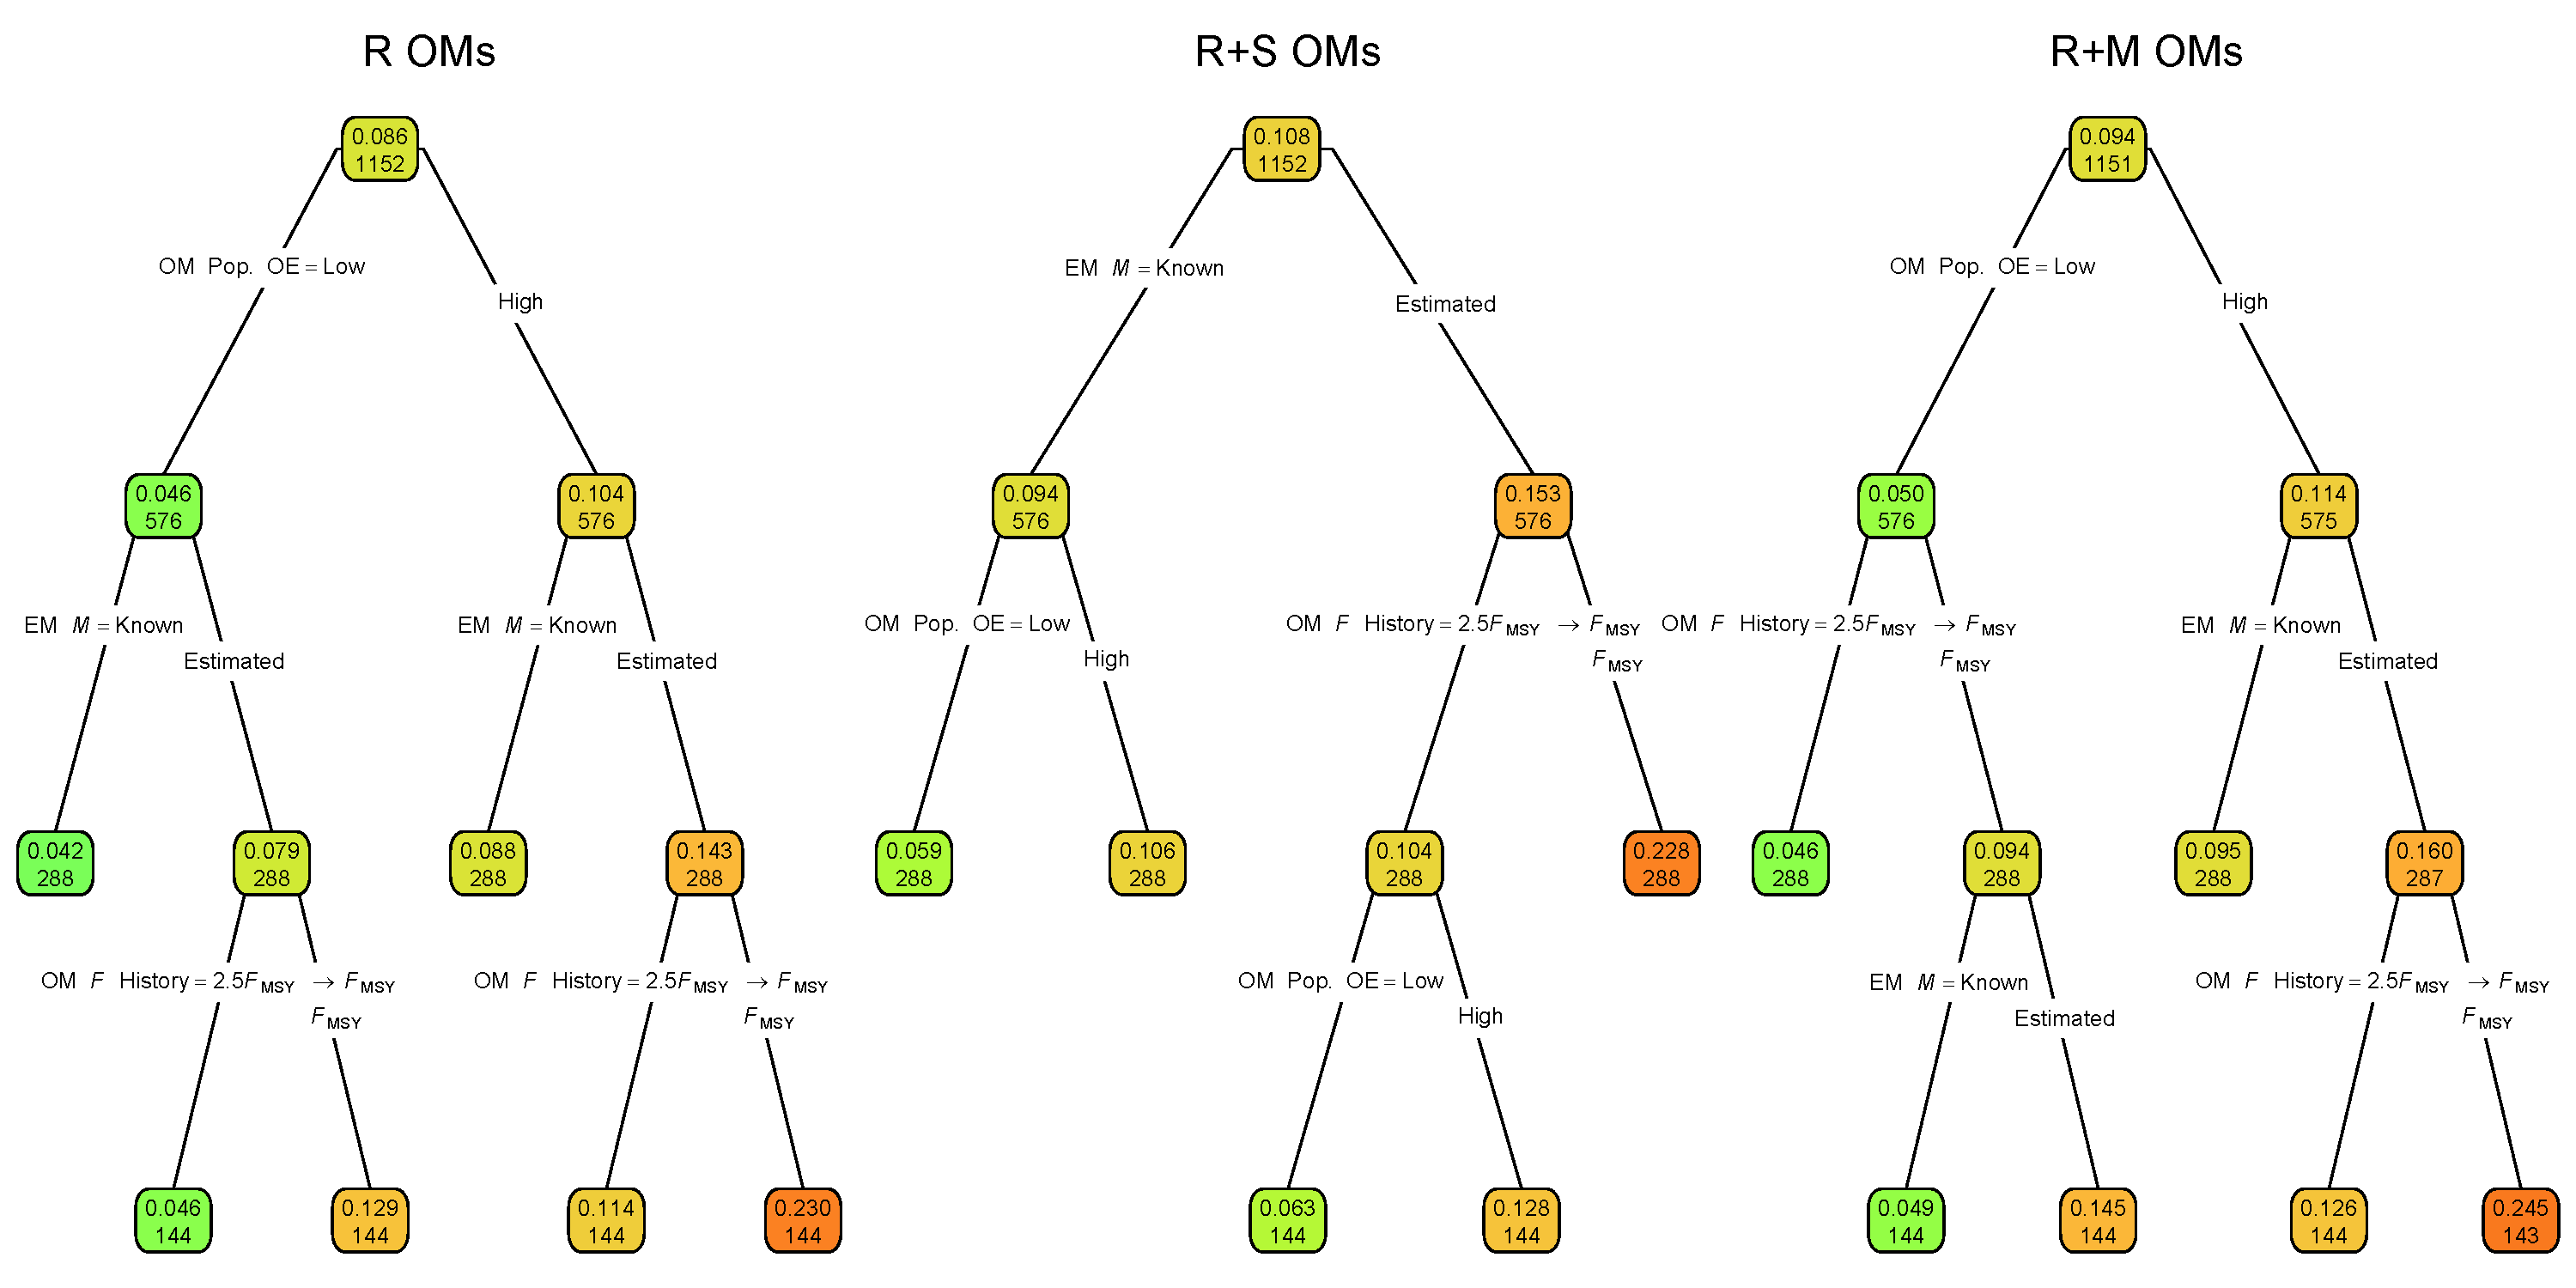
\includegraphics[width = 1.4\textwidth]{term_F_rmse_regtree_plots}
\end{center}
\caption{Regression trees for the log-transformed RMSE of terminal year fishing mortality rate. Each node shows the median error for the corresponding subset. Lower or higher median RMSE is indicated by more green or red polygons, respectively. See Figure \ref{conv_class} caption and Table \ref{factor_table} for further details.}\label{term_F_rmse_regtree}
\end{figure}
\end{landscape}

\begin{table}
\caption{Percent reduction in deviance for linear regression models fit to log-transformed RMSE of terminal year fishing mortality rate. See Tables \ref{convergence_PRD_table} and \ref{factor_table} for further details.}\label{rmse_F_PRD_table}
{\input{rmse_F_PRD_table}}
\end{table}
\pagebreak

\begin{landscape}
\begin{figure}
\begin{center}
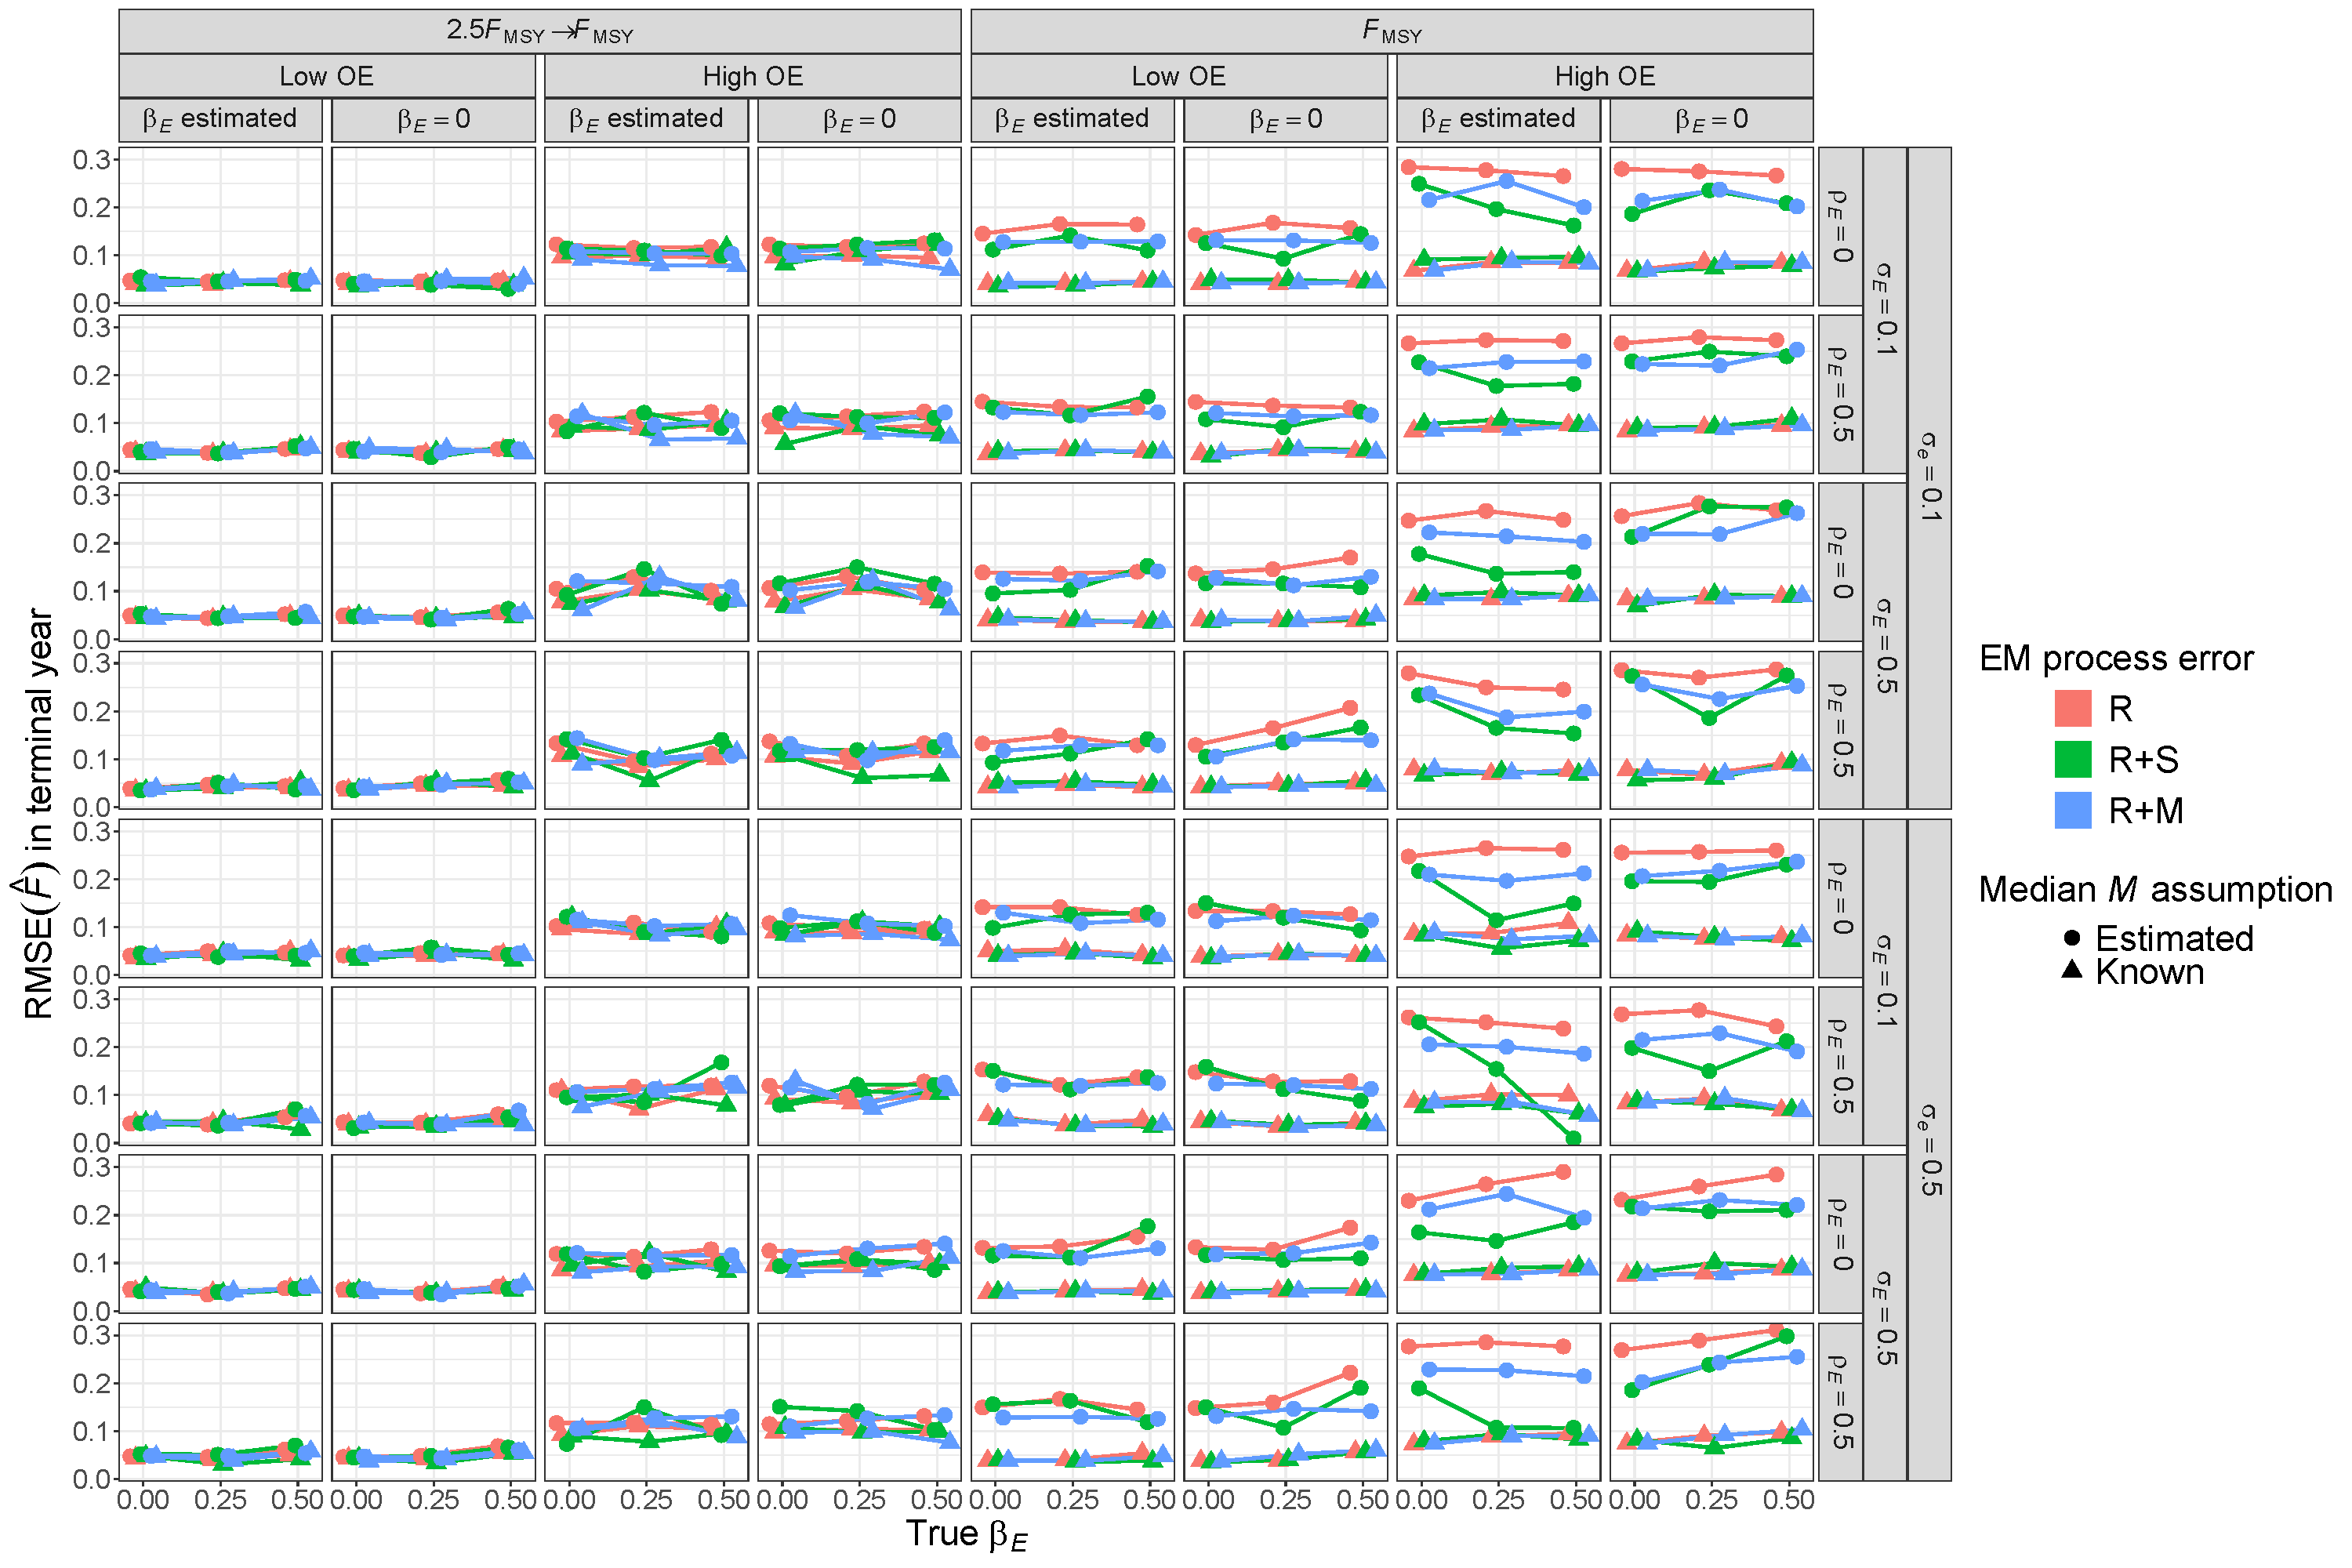
\includegraphics[height = \textheight]{terminal_year_F_rmse_Rom}
\end{center}
\caption{For R operating models, RMSE of estimates of fully-selected fishing mortality ($F$)  in the terminal year for estimating models with alternative process error assumptions, treatment of covariate effect ($\beta_E = 0$ or estimated), and treatment of median $M$ parameter ($\beta_M$ estimated or known).}\label{terminal_F_rmse_Rom}
\end{figure}
\end{landscape}

\begin{landscape}
\begin{figure}
\begin{center}
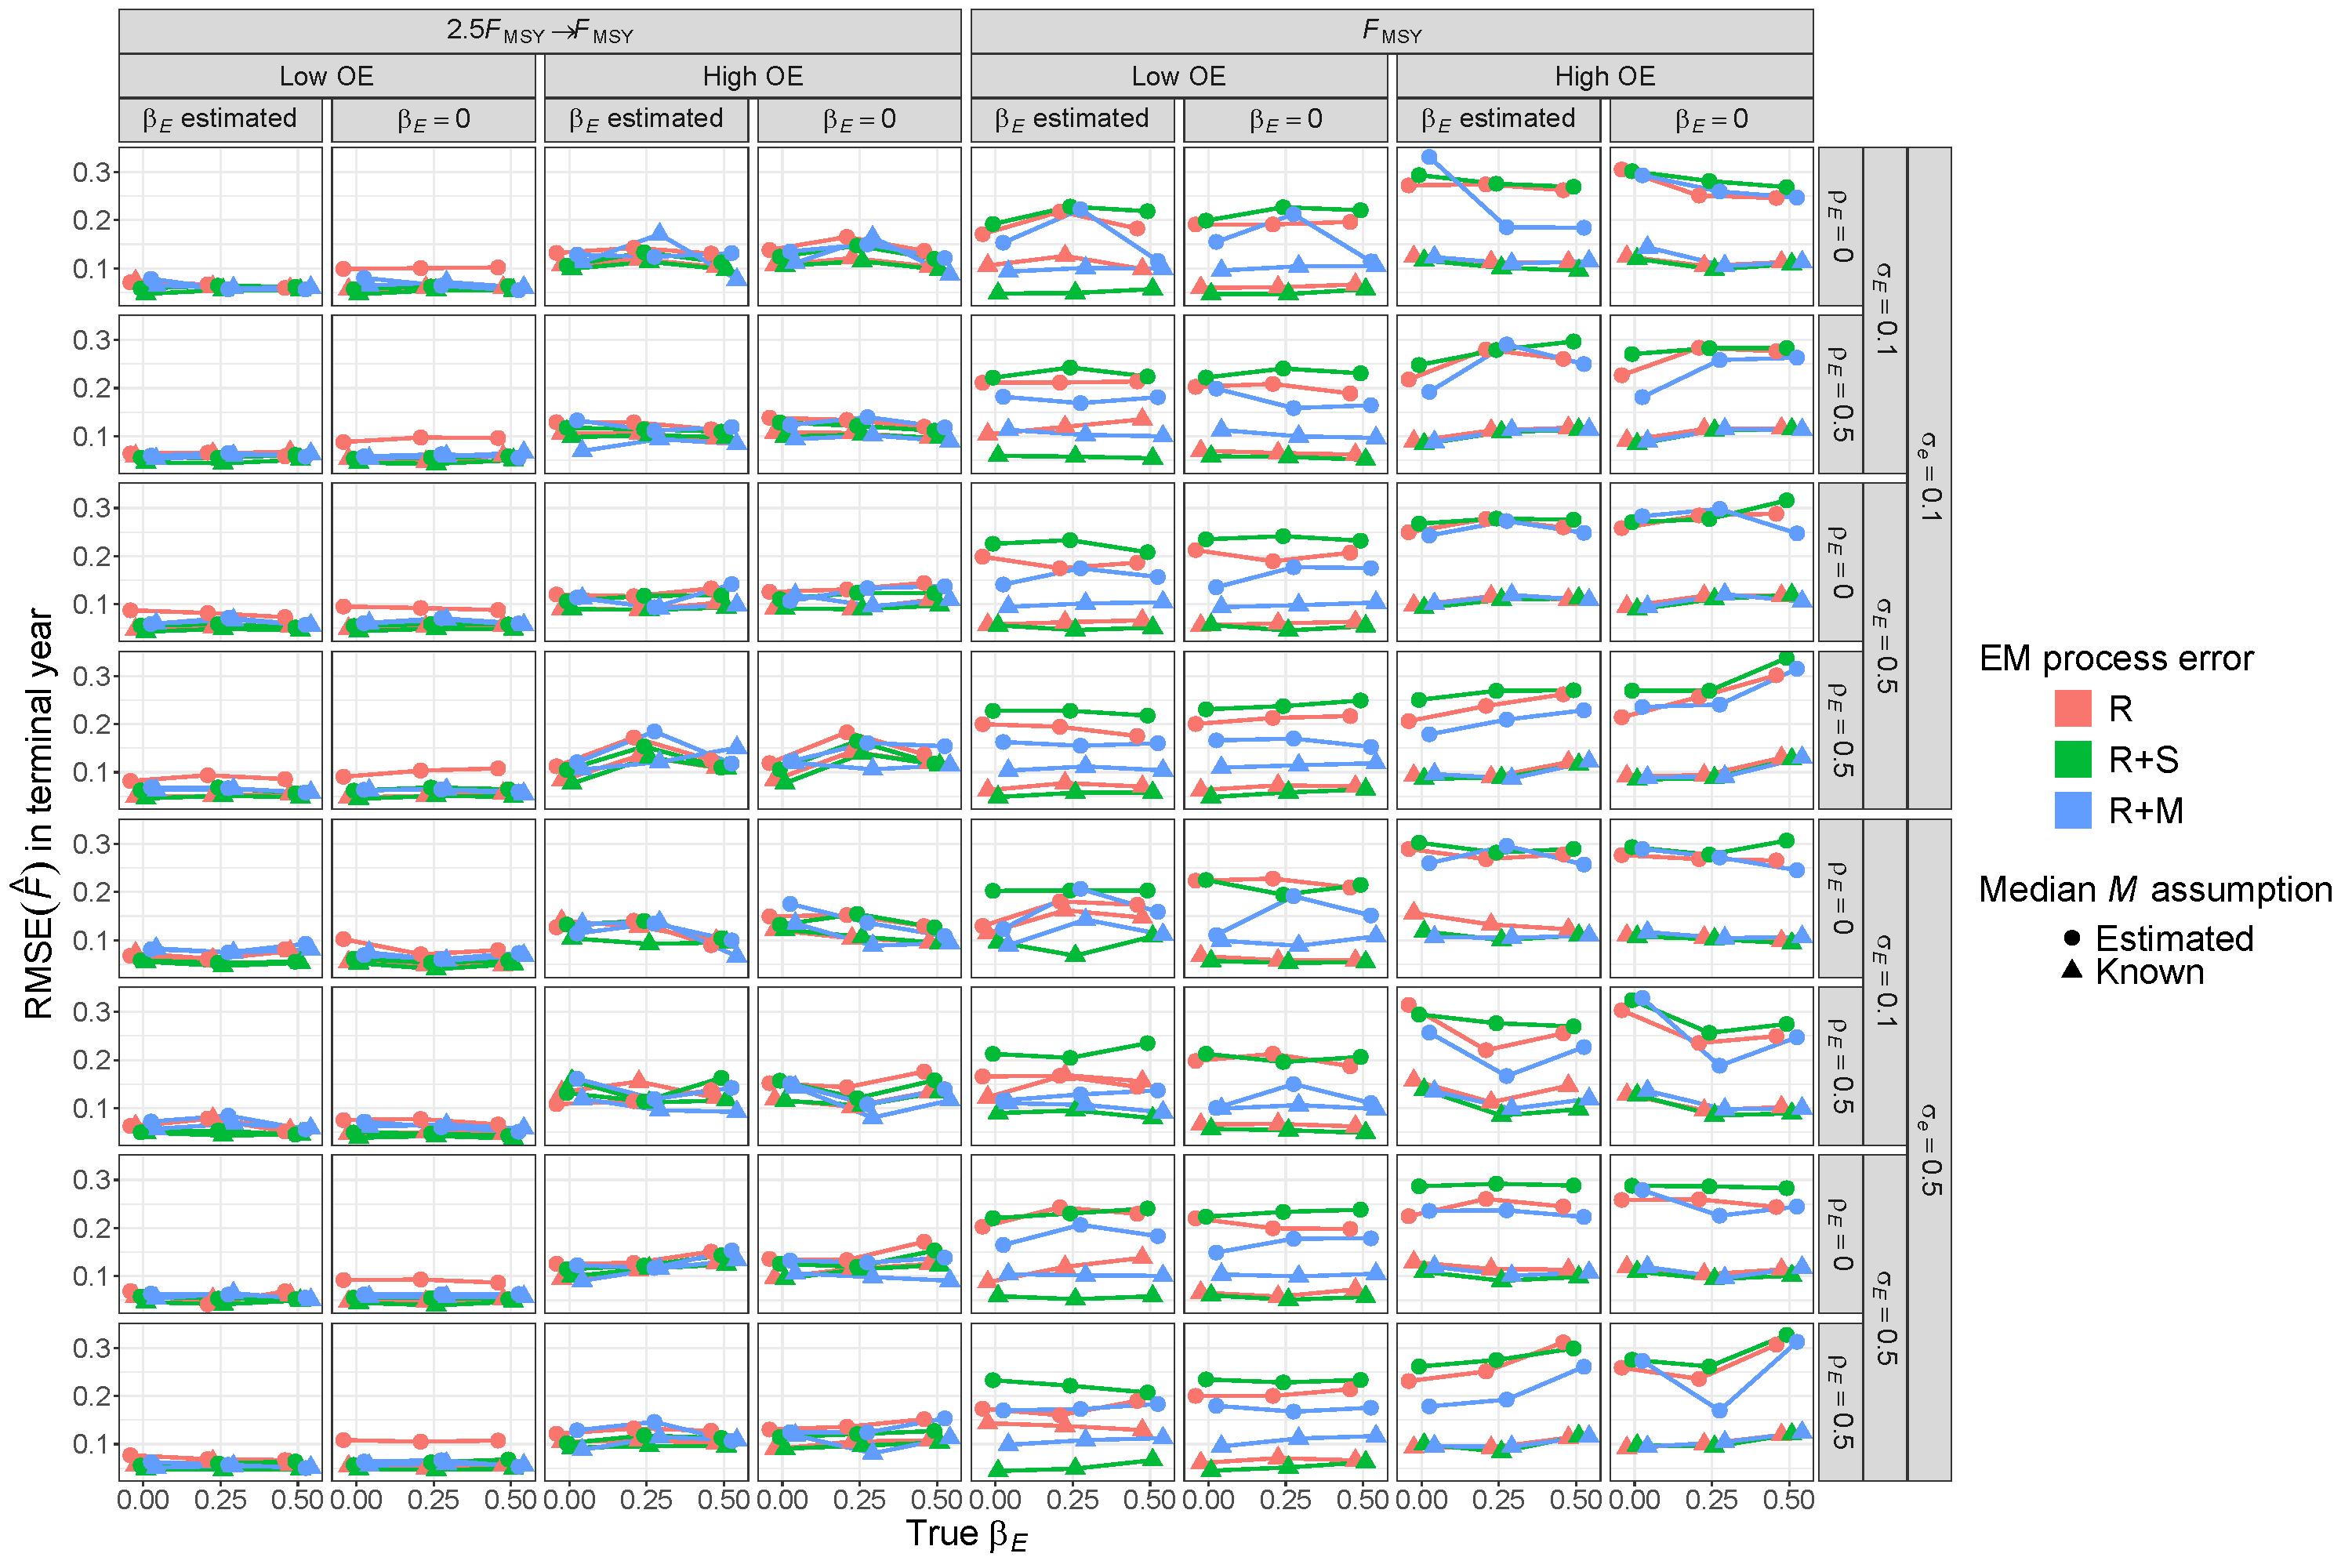
\includegraphics[height = \textheight]{terminal_year_F_rmse_RSom}
\end{center}
\caption{For R+S operating models, RMSE of estimates of fully-selected fishing mortality ($F$)  in the terminal year for estimating models with alternative process error assumptions, treatment of covariate effect ($\beta_E = 0$ or estimated), and treatment of median $M$ parameter ($\beta_M$ estimated or known).}\label{terminal_F_rmse_RSom}
\end{figure}
\end{landscape}

\begin{landscape}
\begin{figure}
\begin{center}
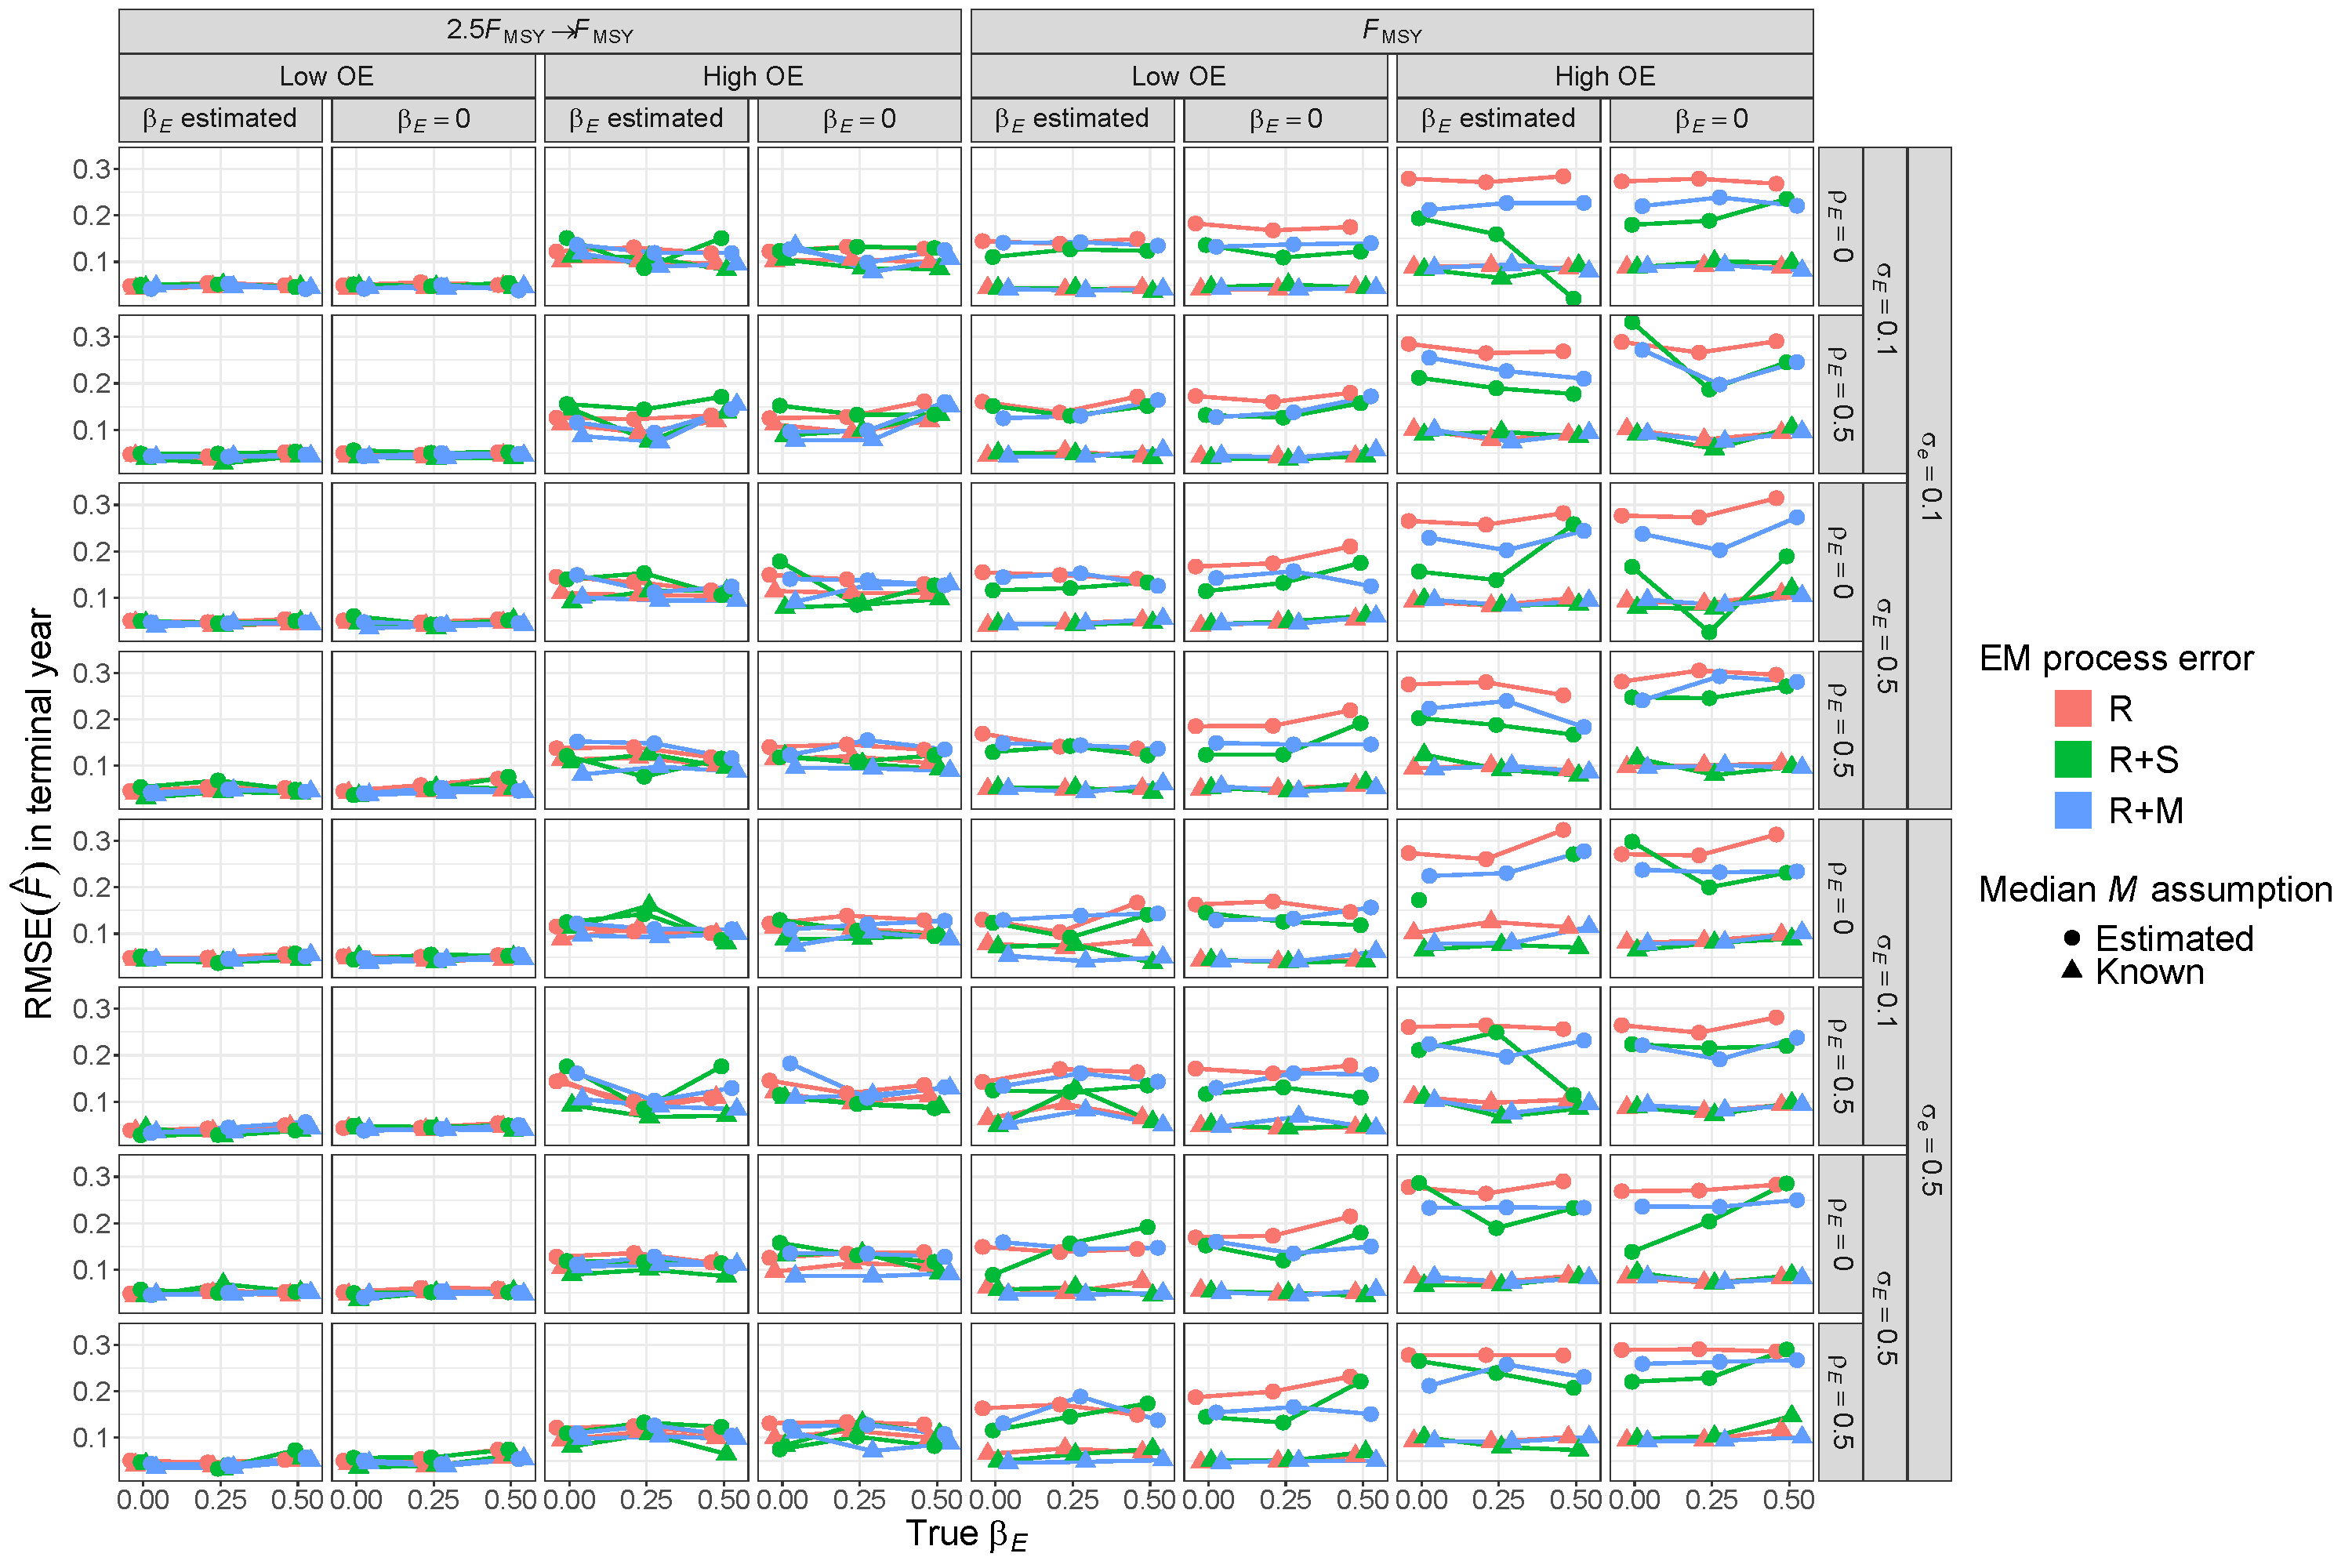
\includegraphics[height = \textheight]{terminal_year_F_rmse_RMom}
\end{center}
\caption{For R+M operating models, RMSE of estimates of fully-selected fishing mortality ($F$)  in the terminal year for estimating models with alternative process error assumptions, treatment of covariate effect ($\beta_E = 0$ or estimated), and treatment of median $M$ parameter ($\beta_M$ estimated or known).}\label{terminal_F_rmse_RMom}
\end{figure}
\end{landscape}

\end{document}
